\documentclass[12pt,a4paper,oneside,english]{report}
\special{papersize=210mm,297mm}
%\usepackage[T1]{fontenc}
%\usepackage[latin1]{inputenc}
\usepackage[cm]{fullpage}
\usepackage[english]{babel}
\usepackage[pdftex]{graphicx}
\usepackage[labelsep=period]{caption}
\usepackage{subcaption}
\usepackage{color}
\usepackage{fixltx2e}
\usepackage{epstopdf}
\usepackage{hyperref}
\usepackage{float}
\usepackage{textcomp}
\usepackage{circuitikz}
%\usepackage{subfig}
\graphicspath{{./FIG}}

\begin{document}
\ctikzset{bipoles/length=.6cm}
\ctikzset{bipoles/thickness=4}
\newcommand\electricC {
\hspace{-14 pt}
\begin{circuitikz}
\draw (0,0) to[capacitor] (0:1);
\end{circuitikz}
\hspace{-6 pt}
}
\newcommand\electricR {
\hspace{-14 pt}
\begin{circuitikz}
\draw (0,0) to[european resistor] (0:1);
\end{circuitikz}
\hspace{-6 pt}
}
\newcommand\electricL {
\hspace{-14 pt}
\begin{circuitikz}
\draw (0,0) 
 to[american inductor] (-1,0) 
;\end{circuitikz}
\hspace{-6 pt}
}
\newcommand\electricDAK {
\begin{circuitikz}
\draw (0,0) to[full diode] (0:1);
\end{circuitikz}
}
\newcommand\electricDKA {
\begin{circuitikz}
\draw (0,0) to[full diode] (180:1);
\end{circuitikz}
}
\title{TransistorTester with AVR microcontroller \\
and a little more\\
Version 1.12k \\
}
\author{Karl-Heinz K\"ubbeler\\
\texttt{kh\_kuebbeler@web.de}}
\date{\today}
\maketitle
\tableofcontents

\section*{Vorwort}

\subsection*{Grundsätzliches}
Jeder Bastler kennt das folgende Problem: Man baut einen Transistor aus oder man nimmt einen aus einer Bastelkiste.
Wenn man die Typenbezeichnung erkennen kann und man bereits ein Datenblatt hat oder eins bekommen kann, ist alles in Ordnung.
Aber wenn man keine Datenblätter findet, hat man keine Idee, was das für ein Bauteil sein kann.
Mit den konventionellen Messmethoden ist es schwierig und zeitaufwändig den Typ des Bauteils und dessen Parameter herauszufinden.
Es könnte ein NPN, PNP, N- oder P-Kanal-MOSFET usw. sein. 
Es war die Idee von Markus F., diese Arbeit von einem AVR-Mikrocontroller erledigen zu lassen.

\subsection*{Wie meine Arbeit begann}
Meine Beschäftigung mit der Software des TransistorTesters von Markus F. \cite{Frejek} hat begonnen, als ich Probleme mit
meinem Programmer hatte.
Ich hatte eine Platine und Komponenten gekauft, aber ich war mit dem Windows-Treiber nicht in der Lage den EEPROM des ATmega8
ohne Fehlermeldungen zu beschreiben.
Deshalb habe ich die Software von Markus F. genommen und habe alle Zugriffe auf den EEPROM-Speicher durch
Zugriffe auf den Programm-Speicher (Flash) ersetzt.
Bei der Durchsicht der Software, um an anderer Stelle Programmspeicher einzusparen, hatte ich die Idee,
das Ergebnis der ReadADC-Funktion von ADC-Einheiten in eine Millivolt (mV) Auflösung zu ändern.
Die mV-Auflösung wird für die Ausgabe von Spannungswerten gebraucht.
Wenn die ReadADC-Funktion direkt die mV-Auflösung liefert, kann man die Umwandlung für jeden Ausgabewert einsparen.
Diese mV-Auflösung kann man erhalten, wenn man zuerst die Ergebnisse von 22 ADC-Einlesungen addiert.
Die Summe muss mit Zwei multipliziert und durch Neun geteilt werden.
Das ergibt einen Maximalwert von \begin{math}\frac{1023\cdot22\cdot2}{9} = 5001\end{math},
welcher hervorragend zu der gewünschten mV-Auflösung passt.
So hatte ich zusätzlich die Hoffnung, dass die Erhöhung der ADC-Auflösung durch Überabtastung helfen
könnte, die Spannungs-Einlesung zu verbessern, wie es in dem Atmel-Report AVR121 \cite{AVR121} beschrieben ist.
Die Original-Version von ReadADC hat die Ergebnisse von 20 ADC-Einlesungen addiert und danach durch 20 dividiert,
so dass das Ergebnis wieder die Original-Auflösung des ADC hat. Deshalb konnte niemals eine Erhöhung der ADC-Auflösung
durch Überabtastung stattfinden.
So hatte ich wenig Arbeit, die ReadADC-Funktion zu ändern, aber dies erforderte die Analyse des kompletten
Programms und Änderung aller ,,if''-Abfragen im Programm, wo Spannungswerte geprüft wurden.
Aber dies war nur der Beginn meiner Arbeit!

Mehr und mehr Ideen wurden eingebaut, um die Messung schneller und genauer zu machen.
Zusätzlich wurde der Bereich der Widerstands- und Kondensator-Messung erweitert.
Das Ausgabe-Format für das LC-Display wurde verändert, so wurden Symbole für die Darstellung von
Dioden, Widerständen und Kondensatoren verwendet.
Für weitere Einzelheiten schauen Sie in das aktuelle Eigenschaften-Kapitel \ref{sec:features}.
Geplante Arbeiten und neue Ideen wurden im Arbeitslisten-Kapitel \ref{sec:todo} gesammelt.
Inzwischen kann ich unter dem Linux-Betriebssystem auch den EEPROM des ATmega8 einwandfrei beschreiben.

Danken möchte ich hier dem Erfinder und Softwareautor Markus Frejek, der mit seinem Projekt die Weiterführung erst
möglich gemacht hat.
Außerdem möchte ich den Autoren der zahlreichen Beiträge im Diskussionsforum danken, die dabei geholfen haben, neue Aufgaben, Schwachstellen und
Fehler zu finden. 
Weiter gilt mein Dank auch Markus Reschke, der mir die Erlaubnis gegeben hat, seine aufgeräumte Versionen im
SVN-Server zu veröffentlichen. Außerdem sind einige Ideen und Softwareteile von Markus R. in meine Version eingeflossen,
auch hierfür herzlichen Dank.
Auch hat Wolfgang Sch. eine große Leistung vollbracht, das grafische Display mit ST7565-Controller zu unterstützen.
Vielen Dank für den Patch für die 1.10k Softwareversion und für die Integration in die aktuelle Entwicklerversion.
Bedanken möchte ich mich auch bei Asco B., der eine Platine für Nachbauwillige entwickelt hat und bei Dirk W. , der sich
um die Sammelbestellungen für diese Platine gekümmert hat. Ich hätte unmöglich selbst die Zeit dafür aufbringen können, sonst
wäre die Weiterentwicklung der Software noch nicht so weit gekommen.
Auch bei den Mitgliedern des Ortsverbandes Lennestadt des Deutschen Amateur Radio Clubs (DARC) möchte ich mich für zahlreiche
Anregungen und Verbesserungsvorschläge bedanken.
Nicht zuletzt möchte ich mich bei Nick L. aus der Ukraine bedanken, der mich mit Prototyp-Leiterplatten unterstützt hat,
einige Hardware-Erweiterungen vorgeschlagen hat und für die russische Übersetzung dieser Beschreibung gesorgt hat.



%\newpage
\chapter{Eigenschaften}
\label{sec:features}
\begin{enumerate}
\item Arbeitet mit Mikrocontrollern vom Typ ATmega8, ATmega168 oder ATmega328. Auch ATmega644 und ATmega1284 oder ATmega1280 und ATmega2560 können verwendet werden.
\item Anzeige der Messergebnisse auf einem 2x16 oder 4x20 Zeichen großen LC-Display.
 Alternativ kann bei Verwendung eines Prozessors mit mindestens 32K Flash Speicher auch ein graphisches Display
 mit 128x64 Pixel und ST7565-, ST7920, ST7108, KS0108 oder SSD1306-Controller benutzt werden.
 Dabei wird anstelle der Standard 4-Bit Parallel-Schnittstelle
 auch entweder eine 4-Wire SPI-Schnittstelle oder ein I\textsuperscript{2}C-Bus benutzt.
 Sogar Farbdisplays mit ILI9163 oder ST7735 Controller sind mit der SPI-Schnittstelle anschliessbar.
 Für den ST7108 oder KS0108 Controller ist ein seriell-parallel Wandler 74HC(T)164 oder 74HC(T)595 erforderlich,
 da diese Controller nur den 8-Bit parallel Anschluß erlauben.
 Displays mit PCF8812 oder PCF8814 Controller können ohne die großen Transistor-Symbole benutzt werden, da
die Displaygröße unzureichend ist (102x65 und 96x65).
\item Ein-Tasten-Bedienung mit automatischer Abschaltfunktion.
\item Batterie-Betrieb ist möglich, weil der Strom im abgeschalteten Zustand nur etwa 20nA beträgt.
Ab Softwareversion 1.05k wird nach Möglichkeit in den Messpausen der Schlafzustand des ATmega zum Stromsparen benutzt, wenn kein Impulsdrehgeber benutzt wird.
\item Preisgünstige Lösung ist möglich ohne Quarz und ohne automatische Abschaltung.
\item Automatische Erkennung von NPN und PNP bipolaren Transistoren, N- und P-Channel MOSFETs, JFETs,
Dioden, Doppeldioden, N- und P-IGBTs, Thyristoren und Triacs.
Für Thyristoren und Triacs müssen die Zünd- und Halteströme für die richtige Erkennung erreicht werden können.
Bei IGBTs muß die Gate Schwellwertspannung unter \(5V\) liegen.
\item Darstellung der Pin-Belegung der erkannten Bauteile.
\item Messung des Stromverstärkungsfaktors und der Basis-Emitter-Schwellspannung für bipolare Transistoren.
\item Darlington-Transistoren können durch die höhere Schwellspannung und durch den hohen Stromverstärkungsfaktor erkannt werden.
\item Automatische Erkennung einer Schutzdiode bei bipolaren Transistoren und bei MOSFETs.
\item Messung der Schwellwert-Spannung, der Gate-Kapazität  und des R\textsubscript{DSon} bei einer Gatespannung von knapp \(5V\) von MOSFETs.
\item Bis zu zwei Widerstände werden gemessen und mit den \mbox{\electricR} Symbolen
und den Widerstands-Werten mit bis zu vier Dezimalstellen in der richtigen Dimension angezeigt.
Alle Symbole werden eingerahmt mit den gefundenen Testpin Nummern des Testers (1-3).
Deshalb können auch Potentiometer gemessen werden. Wenn der Schleifer eines Potentiometers auf eine Endposition
gestellt ist, kann der Tester nicht mehr zwischen mittlerem Anschluss und Endanschluss unterscheiden.
\item Die Auflösung der Widerstandsmessung ist jetzt bis zu \(0,01\Omega\), Werte von bis zu \(50M\Omega\) werden erkannt.
\item Ein Kondensator kann erkannt und gemessen werden. Der wird mit dem Symbol \mbox{\electricC}
und dem Kapazitätswert mit bis zu vier Dezimalstellen in der richtigen Dimension angezeigt.
Der Wert kann zwischen \(25pF\) (bei \(8MHz\) Takt, \(50pF\) bei \(1MHz\) Takt) bis \(100mF\) liegen. Die Auflösung kann bis zu \(1pF\) (bei \(8MHz\) Takt) betragen.
\item Bei Kondensatoren mit einer Kapazität über \(20nF\) wird zusätzlich der äquivalente Serienwiderstand (ESR) des Kondensators
mit einer Auflösung von \(0,01\Omega\) gemessen und mit zwei Dezimalstellen angezeigt.
Diese Fähigkeit steht nur zur Verfügung, wenn der ATmega mindestens 16K Flashspeicher besitzt.
\item Für Kondensatoren mit einem Kapazitätswert über \(5000pF\) kann der Spannungsverlust Vloss nach einem Ladepuls bestimmt werden.
Der Spannungsverlust gibt einen Hinweis auf die Güte des Kondensators.
\item Bis zu zwei Dioden werden mit dem Symbol \mbox{\electricDAK} oder dem Symbol \mbox{\electricDKA}
in der richtigen Reihenfolge angezeigt.
Zusätzlich werden die Schwellspannungen angezeigt.
\item Eine LED wird als Diode erkannt, die Schwellspannung ist viel höher als bei einer normalen Diode.
Doppeldioden werden als zwei Dioden erkannt.
\item Zener-Dioden können erkannt werden, wenn die Zener-Spannung unter \(4,5V\) ist.
Sie werden als zwei Dioden angezeigt, man kann das Bauelement nur mit den Spannungen erkennen.
Die äußeren Testpin-Nummern, welche die Dioden Symbole umgeben, sind in diesem Fall identisch.
Man kann die wirkliche Anode der Diode nur durch diejenige Diode herausfinden, deren Schwellwert-Spannung nahe bei \(700mV\) liegt!
\item Wenn mehr als 3 Dioden erkannt werden, wird die gefundene Anzahl der Dioden zusammen mit der Fehlermeldung angezeigt.
Das kann nur passieren, wenn Dioden an alle drei Test-Pins angeschlossen sind und wenigstens eine eine Zener-Diode ist.
In diesem Fall sollte man nur zwei Test-Pins anschließen und die Messung erneut starten, eine Diode nach der anderen.
\item Der Kapazitätswert einer einzelnen Diode in Sperr-Richtung wird automatisch ermittelt.
Bipolare Transistoren können auch untersucht werden, wenn nur die Basis und entweder Kollektor oder Emitter angeschlossen wird.
Bei ATmega mit mehr als 16k Flash Speicher wird außerdem der Sperrstrom mit einer Auflösung von \(2nA\) gemessen.
Der Wert wird nur ausgegeben, wenn er nicht null ist.
\item Die Anschlüsse einer Gleichrichter-Brücke können mit nur einer Messung herausgefunden werden.
\item Kondensatoren mit Kapazitätswerten von unter \(25pF\) werden normalerweise nicht erkannt, 
aber sie können zusammen mit einer parallel geschalteten Diode oder mit einem parallel geschaltetem Kondensator mit
wenigstens \(25pF\) gemessen werden.
In diesem Fall muss der Kapazitätswert des parallel geschalteten Bauteils vom Messergebnis abgezogen werden.
Bei Prozessoren mit mindestens 32K Flash Speicher wechselt der Tester mit einem Kondensator \textgreater~\(25pF\)
an TP1 und TP3 in eine Kondensator-Meßfunktion, die auch Kapazitäten ab \(1pF\) direkt mißt.
\item Bei Widerständen unter \(2100\Omega\) wird auch eine Induktivitätsmessung durchgeführt, wenn der
ATmega wenigstens 16K Flashspeicher besitzt.
Dabei wird zusätzlich zum Widerstands-Symbol \mbox{\electricR} ein Induktivitäts Symbol \mbox{\electricL} angezeigt.

Der Anzeigebereich ist etwa \(0,01mH\) bis über \(20H\), die Genauigkeit ist allerdings nicht hoch.
Das Ergebnis wird nur bei einem Einzelwiderstand zusammen mit dem Widerstandswert angezeigt.
\item Die Messzeit beträgt ungefähr zwei Sekunden, nur Kapazitätsmessungen und Induktivitätsmessungen können länger dauern.
\item Die Software kann für Messserien mit vorgebbarer Wiederhol-Zahl konfiguriert werden, bevor die automatische Abschaltung ausschaltet.
\item Eingebaute Selbsttest-Funktion inklusive einem optionalen \(50Hz\) Frequenz-Generator um die Genauigkeit der Taktfrequenz
und der Verzögerungszeiten zu überprüfen (nur mit mindestens 16K Flash Speicher).
\item Wählbare Möglichkeit den Nullabgleich für die Kondensatormessung und die Innenwiderstände für die
Portausgänge beim Selbsttest automatisch zu bestimmen (nur mit mindestens 16K Flash Speicher).
Ein externer Kondensator mit einer Kapazität zwischen \(100nF\) und \(20\mu F\) an Pin~1 und Pin~3 ist notwendig, 
um die Offset-Spannung des analogen Komparators zu kompensieren.
Dies kann den Messfehler bei Kapazitätsmessungen bis zu \(40\mu F\) reduzieren.
Mit dem gleichen Kondensator wird eine Korrekturspannung zum Einstellen der richtigen Verstärkung für
die ADC Messung mit der internen \(1,1V\) Referenzspannung berechnet.
\item Anzeige des Kollektor-Emitter-Reststroms \(I_{CE0}\) mit stromloser Basis (\(1\mu A\) Auflösung) und
des Kollektor-Emitter Reststroms \(I_{CES}\) mit der Basis auf Emitter-Potential gehalten (nur bei mindestens 16K Flash).
Diese Werte werden nur angezeigt, wenn sie nicht Null sind (besonders für Germanium-Transistoren).
\item Für ATmega mit mindestens 32K Flash-Speicher wechselt der Tester vom Multifunktionstest zu einem Modus als
Widerstands-Meßgerät, wenn bei der automatischen Bauteile-Erkennung nur ein Widerstand an Test Pin 1 (TP1) und
Test Pin 3 (TP3) erkannt wird. Wenn in der Makefile auch die Induktivitätsmessung beim Widerstandsmeßgerät
mit der Option RMETER\_WITH\_L gewünscht wurde, werden bei der Widerstandsmessung auch Induktivitäten gemessen.
Der Betriebsmodus wird durch {\bf[R]} oder {\bf[RL]} auf der rechten Seite von Zeile 1 des Displays angezeigt.
Genau so wechselt der Tester zu einem Kapazitätsmeßgerät, wenn bei der Bauteile-Untersuchung
eine Kondensator an TP1 und TP3 erkannt wurde. Dieser Betriebsmodus wird durch {\bf[C]} auf der rechten Seite der Zeile 1 angezeigt.
In dieser Betriebsart können Kondensatoren ab \(1pF\) gemessen werden. Lediglich für den automatischen Start der Funktion
braucht man einen Kondensator mit mehr als \(25pF\).
Beide Sonderfunktionen können durch einen Tastendruck wieder beendet werden. Der Tester fährt dann mit der normalen
Meßfunktion fort.
\item Für Prozessoren mit mindestens 32K Flash kann eine Dialogfunktion gewählt werden, 
die weitere Einsatzmöglichkeiten zugänglich machen kann.
Natürlich kann über den Dialog auch zu der Transistortester-Funktion zurückgekehrt werden.
\item Mit Dialogfunktion kann am PD4-Port des ATmega eine Frequenzmessung vorgenommen werden.
Die Auflösung beträgt bei Eingangfrequenzen über \(25kHz\) ein Hertz.
Bei niedrigeren Frequenzen kann die Auflösung bis zu \(0,001mHz\) betragen.
Lesen Sie bitte das Unterkapitel \ref{sec:frequency_counter} auf Seite \pageref{sec:frequency_counter},
wie ein Frequenzsignal angeschlossen werden muß.
\item Mit Dialogfunktion und ohne serielle Ausgabe kann eine externe Spannung bis \(50V\) über einen
10:1 Spannungteiler am PC3 Pin gemessen werden. Bei der PLCC-Version des ATmega328 kann auch einer der beiden
zusätzlichen Pinne für die Spannungsmessung zusammen mit der seriellen Ausgabe benutzt werden.
Wenn die Erweiterung für die Zenerdiodenmessung (DC-DC-Konverter)
eingebaut ist, können in diesen Zweig auch Zenerdioden bei gedrückter Taste getestet werden.
\item Mit Dialogfunktion kann eine Frequenzausgabe auf dem TP2-Pin (PB2-Port des ATmega) erfolgen.
Derzeit ist eine Auswahl von Frequenzen von \(1Hz\) bis \(2MHz\) wählbar.
\item Mit Dialogfunktion kann eine feste Frequenz mit einstellbarer Pulsweite auf dem TP2-Pin (PB2-Port des ATmega)
ausgegeben werden.
Die Breite kann mit kurzem Tastendruck um \(1\%\) und mit längerem Tastendruck um \(10\%\) erhöht werden.
\item Mit der Dialogfunktion kann eine spezielle Kondensatormessung mit ESR-Messung gestartet werden.
Die Funktion wird bei der Auswahl \mbox{C+ESR@TP1:TP3} genannt.
 Kapazitäten ab etwa \(2\mu F\) bis zu \(50mF\) können meistens wegen der geringen Messspannung von etwa \(300mV\)
 im eingebauten Zustand gemessen werden.
\item Bei Prozessoren mit mindestens 32K Flash-Speicher (Mega328) kann der ADC mit der Sampling-Methode so genutzt werden,
daß Kondensatoren unter 100pF mit einer Auflösung von 0.01pF gemessen werden können. Mit der gleichen Methode können
auch Spulen unter 2mH mit deutlich besserer Auflösung über die Resonanzfrequenz mit einem parallelgeschalteten Kondensator 
bekannter Größe bestimmt werden.

\end{enumerate}

 Bei Einsatz des Testers für die Prüfung von Kondensatoren in einer Schaltung sollte besonders darauf geachtet werden,
 dass die Kondensatoren vor der Messung keine Restladung mehr haben.


Thyristoren und Triacs können nur erkannt werden, wenn der Test-Strom über dem Halte-Strom liegt.
Einige Thyristoren und Triacs brauchen auch einen höheren Zündstrom als dieser Tester liefern kann.
Der verfügbare Teststrom ist nur ungefähr \(6mA\)!
Ebenso können IGBTs nur erkannt werden, wenn eine Spannung von \(5V\) für die Gate-Ansteuerung reicht.
Beachten Sie bitte, dass viele Möglichkeiten nur für Mikrocontroller mit wenigstens 16K Programmspeicher wie ATmega168 zur Verfügung stehen. 
Alle Eigenschaften sind sogar nur für Prozessoren mit wenigstens 32K Programmspeicher wie ATmega328 oder ATmega1284 möglich.

\vspace{1cm}
\textbf{{\Large Achtung:}} Stellen Sie immer sicher, dass {\bf Kondensatoren} vor dem Anschluss an den Tester {\bf entladen} sind!
Der Tester könnte sonst beschädigt werden bevor er eingeschaltet ist.
Es gibt nur wenig Schutzfunktion der ATmega-Anschlüsse.
Besondere Vorsicht ist auch geboten, wenn versucht wird, Bauelemente in einer Schaltung zu messen.
Das Gerät sollte in jedem Fall vorher von der Strom\-ein\-spei\-sung getrennt sein und man sollte sicher sein,
dass {\bf keine Restspannung} im Gerät vorhanden ist.




\chapter{Hardware}

\section{Circuit of the TransistorTester}
\label{sec:hardware}
The circuit of the TransistorTester in figure \ref{fig:ttester} is based on the circuit of
 Markus F. released in Abb.~1 of AVR-Transistortester report \cite{Frejek}.
Changed or moved parts are marked with green color, optional parts are marked with red color.

Some changes are made because the electronical power switch make problems in some implementations.
Therefore the resistor R7 is reduced to \(3.3k\Omega\). The capacitor C2 is reduced to
10nF and R8 is moved so that the PD6 output does not try to switch the C2 capacitor directly.
 Additional blocking capacitors are added and should be placed
near the power connection of the Atmega and near the Voltage regulator.

Because the PD7 input and PC6 (RESET) are the only pins, where pull up resistors where
needed, one extra \(27k\Omega\) resistor is added to the PD7 (pin~13) input. With this modification
the software can disable all internal pull up resistors of the ATmega.

The additional crystal with its 22pF capacitors are optional added. 
The accuracy of a crystal has the benefit of more stable time measurement for getting the
capacitor values.

New software version can use a voltage scale switch of the ADC. The speed of switching is reduced
by the external capacitor C1 at the AREF (21) pin of the ATmega. To avoid slowing down the
measurement speed more than necessary, the value of this capacitor should be reduced to 1nF.
Removing of the capacitor C1 is also possible.
For adapting the software to the actual circuit take a look to the Makefile options in the
configuring chapter \ref{sec:config}.

Some different versions of R11 / R12 resistor combinations circulates
in the internet. I~have adapted my software to the original of Markus F. \cite{Frejek} with \(10k\Omega\) and \(3.3k\Omega\).

The additional 2.5V precision voltage reference connected at pin PC4 (ADC4) can be used to
check and calibrate the VCC voltage, but is not required.
A optional ISP connector has been added to easier load new software versions to the tester.

\begin{figure}[H]
\centering

\includegraphics[width=18cm]{../FIG/ttester.eps}
\caption{New circuit of TransistorTester}
\label{fig:ttester}
\end{figure}
The software can follow to another pin assignment of port D for a simpler connection of the
LCD display. 
The following table \ref{tab:grid-change} shows the modified assignments.

\begin{table}[H]
  \begin{center}
    \begin{tabular}{| c | c | c |}
    \hline
       Signal & circuit diagram & strip grid board version\\
    \hline
    pushbutton input  &  PD7   &  PD0 \\
    LCD-RS    &  PD4      & PD7 \\
    LCD-E     &  PD5   & PD5 \\
    LCD-D4    &  PD0   & PD4 \\
    LCD-D5    &  PD1   & PD3 \\
    LCD-D6    &  PD2   & PD2 \\
    LCD-D7    &  PD3   & PD1 \\
    \hline
    \end{tabular}
  \end{center}
  \caption{Changes for strip grid board}
  \label{tab:grid-change}
\end{table}

For better protection of the ATmega inputs the additional circuit~ \ref{fig:relay_addon} 
can be integrated. The de-energized contacts of the relay protect the ATmega without power.
The contacts will be opened by software only for measurement.

\begin{figure}[H]
\centering

\includegraphics[width=7cm]{../FIG/relay_addon.eps}
\caption{Additional protection of the ATmega inputs}
\label{fig:relay_addon}
\end{figure}

If the serial output of text is not required, the Pin PC3 of the ATmega can be used as analog
input for measuring a external voltage. The voltage can be up to 50V with the optional 10:1 resistor
divider and can be used for measuring the breakdown voltage of a zener diode. 
A current limiting power supply with up to 50V can be switched on with low signal at PD7 pin of the
ATmega to deliver current for testing the break down voltage of a zener diode.
Figure~\ref{fig:zener} shows a suggestion for this expansion.
The tester shows the external voltage as long as you hold the key pressed.
About 40mA more battery current is used by this expansion during key pressing.

\begin{figure}[H]
\centering

\includegraphics[width=12cm]{../FIG/zener_exp.eps}
\caption{Expansion for measuring of break down voltage of Zener diodes}
\label{fig:zener}
\end{figure}




\section{Hints for building the TransistorTester}
Every LCD-display with at least 2x16 character and a HD44780 compatible controller
can be used with the TransistorTester. You should respect the current needed for
illumination, some LCD need lower current than others.
I had tried OLED type displays, but this type cause interference with measurements
of the ATmega and are {\bf not} recommended. Also loading of special characters
for displaying the resistor symbol has caused problems with the OLED.

The resistors R1 to R6 are critical for measurements and this \(680\Omega\) and
\(470k\Omega\) resistors should be measurement type resistors (tolerance of 0.1\%) to
get the full accuracy.
You should use a precision socket for the ATmega microcontroller to enable
the replacement of the microcontroller.
The microcontroller ATmega8, ATmega168 and ATmega328 can be used.
Recommended is a ATmega168 or ATmega328, if you wish to use all features.

Anyway you should assemble all parts to printed board without the microcontroller.
A up-to-date low voltage drop regulator like MCP1702-5002 is recommended as IC2, because it
need only \(2\mu A\) of standby current and can still deliver 5V, if your input
voltage is only 5.4V. But this part is not pin compatible to well known 78L05 with TO92 body!

After checking, that all needed parts are at the correct place, you should
first connect the battery or power supply to the printed board without LCD-display
and microcontroller. You should check the voltage at the power pins of the
microcontroller and LCD-display terminal during the Test key is pressed.
The voltage should disappear, if you release the Test key.
If the voltage had correct polarity and value,
you should disconnect the power and assemble the microcontroller with correct
alignment. Be careful and make shure, that all pins of the microcontroller
are in the socket holes.
Now you can also connect the LCD. Check if power pins of the LCD has the right connection to
GND and VCC of your board.

If you are shure that everything is all right, reconnect the power. 
If you have already programmed the ATmega, you can press the Test button.
By pressing the Test key, the background light of the LCD should switch on.
If you release the Test button, the LED should illuminate weak.
Notice, that the software for the microcontroller must be compiled for the
correct processor type. A program for the ATmega8 does not run on a ATmega168!

\section{Changeover for tester versions designed by Markus F.}
\label{sec:change_markus}
\begin{description}

\item[Voltage control]
If the problem exist, the tester will shut down immediately with every switch on.
With imy suggested setting of the fuses (Makefile) the voltage control of the different
ATmega versions is switched to 4V (brown out level).
This may be the reason why the tester makes trouble with the power on sequence.
The Pin PD6 tries to switch the 100nF capacitor C2 to VCC level causing a voltage
breakdown of the VCC voltage (5V).
The capacitor C2 can be reduced to \textless 10nF without problems.
If possible, the direct connection of PD6 should be replaced by a resistor \textgreater \(220 \Omega\).
\item[Improvement of power on circuit]
Often this problem is the reason, if the tester starts with the button hold pressed, but switch off
directly by releasing. The problem is enforced by a high current background light for the LCD.
The resistor R7 to the base of the PNP transistor T3 was optimized with the value \(27k \Omega\) 
too much to save power consuming.
To improve the switching with lower battery voltage or lower current amplification factor of
the PNP transistor T3, you should reduce the resistance to \(3.3k \Omega\).
\item[Additional pull-up resistor at PD7]
The missing pull-up resistor results to a switch off of the tester with the message ''Timeout''
after a short display time.
The software is configured with the option PULLUP\_DISABLE, that all internal pull-up
resistors are switched off. For that reason the voltage of pin PD7 is not definded,
if the level is not switched by the push button or transistor T2 to GND.
One external pull-up resistor of \(27k \Omega\) to VCC avoid this error.
\item[Capacitor C1 at the AREF pin]
Many designs use a 100nF capacitor at the AREF pin, like the design of Markus F. too.
As long as the reference voltage of the ADC is never changed, this is a good solution.
The software of the TransistorTester for the ATmega168/328 uses a automatic selection
of the internal 1.1 V reference voltage of the ADC, if the input voltage is below 1V.
With this solution a better resolution of the ADC can be reached for little input voltages.
Unfortunately the switching from 5V to 1.1V reference is very slowly. A additional
wait time of 10ms must be respected for this reason.
With changing the capacity value to 1nF this wait time can be reduced significant.
I have not noticed any degration of measurement quality with this change.
Even a removing of the capacitor has no significant change of measurement results.
If you prefer to leve the capacitor unchanged, you can remove the option NO\_AREF\_CAP
in the Makefile to activate longer wait times in the program.
\item[Expanding of a 8MHz crystal]
With some skill you can expand a 8MHz crystal to the backside of the printed board
directly to the pins PB6 and PB7 (pin 9 and pin 10).
My own expansion was done without the both 22pF capacitors.
This solution has operated well with all tested ATmega.
But it is not required to use a crystal. You can still use the 8MHz RC oszillator
by setting the fuses to get the better resolution of time constant measuring (capacity value).
\item[Smoothing of the operating voltage]
The original circuit of Markus F. shows only one 100nF capacitor to block the VCC voltage.
This is clearly too little smoothing. You should at least use one 100nF near the ATmega power pins
and one near the voltage regulator. The input of the voltage regulator should be
blocked with a 100nF too.
Additional \(10\mu F\) capacitors (electrolytic or ceramic) at the input and
output of the voltage regulator can stable the voltage level.
Ceramic \(10\mu F\) capacitos with SMD mounting form are easier to use for backfitting
and have usually a lower ESR value. 
\item[Selection of the ATmega processor]
The using of the base function of the tester is still possible with a ATmega8.
The flash memory of that device is used near 100\% .
Because the ATmega168 or ATmeg328 processors are pin-compatible to the ATmega8,
I can recommend the replacement.
Actually the price for ATmega328 is so cheap, that there is no reason to take
a ATmega168 type.
With a ATmega168/328 you get the following advantages:
Self test with automatic calibration.\\
Improvement of measurement quality by automatic switching of ADC scale.\\
Measurement of inductors with resistance  below \(2100 \Omega\).\\
Measurement of ESR value of capacitors with value of above  \(2 \mu F\).\\
Using of pin PC4 as serial output.\\
\item[Missing precision voltage reference]
Usually the software should detect the missing voltage reference with the unconnected pin PC4.
In this case no VCC=x.xV message should appear in row 2 of the LCD on power on.
If this message appear without the reference, you should connect a \(2.2k \Omega\) resistor
to the PC4 input and VCC.


\end{description}

\section{Chinese clones}
As I know, the tester is rebuild in China in two versions.
The first model is rebuild from the first design of Markus F. without the ISP port.
The assembled ATmega8 is placed in a socket, so you can replace it with a ATmega168 or ATmega328.
For this version you should consider all the hints of section \ref{sec:change_markus}.
Additional \(100nF\) ceramic cpacitors should be connected near by the VCC-GND and AVCC-GND pins of
the ATmega for better stabilization of the power voltage.
In addition you should notice, that if you expand the board with the additional 8 MHz crystal,
your external ISP programmer must have a external clock for programming.\\

The second version of rebuilded tester is build with SMD components. Also the fix installed ATmega168
is a SMD type with 32TQFP body.
Fortunately on the board is a 10-pole ISP connector provided for the programming.
I have analysed the board version ''2.1 2012/11/06''. One error is the assembly of the part ''D1'',
which should be a precision 2.5V voltage reference. Assembled is only a zener diode.
This part should be removed. You can mount a LM4040AIZ2.5 or LT1004CZ-2.5 precision voltage reference
at this place. A missing voltage reference is noticed by the software, so that you must not install
the voltage reference.
My exemplar was delivered with software version 1.02k. The 10-pole ISP plug was not assembled and I must
install a jumper from ISP pin 6 to ISP pin 10. My programmer expect a GND connection at pin 10, but the
board has GND level only on pin 4 and pin 6 of the ISP.
The label of the ATmega168 was rub away and there was no documentation delivered with the part.
The lock fuses of the ATmega were set, so no readout was possible.
But I could install the software version 1.05k without any problems.
Another user has problems with the same software version 1.05k. This user has the chinese board ''2.2 2012/11/26''.
The software runs only without problems, if a additional \(100nF\) keramic capacitor was placed between
the pin 18-AVCC and 21-GND near by the ATmega.
The software 1.05k uses the sleep state of the ATmega for waiting time. For this reason the current alternates
often and the voltage regulator is stressed more.
Further I have noticed, that the VCC voltage is blocked with a \(100nF\) ceramic capacitor and with a
\(220\mu F\) electrolytic capacitor nearby the 78L05 voltage regulator.
The 9V supply voltage is blocked with the same capacitors, but not at the input of the regulator but
at the emitter of the PNP transistor (parallel with the battery). 
The printed circuit board track from the ATmega168 to the test port is very thin, so that a resistance
of \(100m \Omega\) could be measured for one path. This will be the reason for measuring a resistance
of \(0.3 \Omega\) for two direct connected pins.
The ESR measuring can usually consider this by zero compensation.
The current version of software does not respect this offset for measuring of resistors with low resistance.


\section{Programming of the microcontroller}
I release the software for the microcontroller with source code.
The developement is done with Linux operationg system (Ubuntu) and
is controlled with a Makefile. The Makefile makes shure, that your
software will be compiled with the prior selected Makefile options. Some constellations
are precompiled with the source. Please take a look to the ReadMe.txt file
in the directory Sourcecode/default and to the chapter~\ref{sec:config}.
The result of compilation have the extensions .hex and .eep .
Usually the names will be TransistorTester.hex and TransistorTester.eep .
The .hex file contains the data for the program memory (flash) of the ATmega processor.
The .eep file contains the data for the EEprom memory of the ATmega. Both data files
must be loaded to the correct memory.

Additionally the operating state of the
ATmega processor must be programmed with the ``fuses''.
If you can use my Makefile and additionally the program avrdude \cite{avrdude}, you need no exact
knowledge of the details about the fuses. You have only to type ``make fuses'' if you
have no crystal or ``make fuses-crystal'' if you have installed the 8MHz crystal to your printed board.
With the ATmega168 series of the microcontroller you can also use ``make fuses-crystal-lp'' to use
a crytal with the low power mode.
Never choose the crystal mode of clock generation, if you don't have installed
the 8MHz crystal. If you are not shure with the fuses, leave them as default
set by manufactor and first bring the the tester to operation in this mode.
Maybe your program runs too slow, if you use program data compiled for
8MHz operation, but you can correct this later! But a wrong set of fuses may inhibit
later ISP-programming.
If you use the Windows operating system, the easiest way to get a correct programmed
ATmega is to use the WinAVR package \cite{winavr1},\cite{winavr2}.
With my patch \cite{winavr3} you can also set the fuses by using the Makefile.
Of course the avrdude program must support your programmer and the configuration
in the Makefile must match to your environment.


\section{Troubleshooting}
In most cases of problems you will miss the text output to the LCD-display.
At first you should check, if the LED was illuminated weak, if you release
the Test button. 
\begin{description}

\item[Power does not switch on.]
If the LED is without light and the VCC power has correct
5V voltage during holding the Test button, the microcontroller does not switch the power
correctly. The microcontroller should hold the power by switching the
PD6 output to 5V, which is usually done as one of the first actions.
If you hold the Test key pressed, the power is switched on anyway.
So you can check the value of VCC power and additionally the voltage value
of the PD6 output, if you hold the key pressed.
If VCC voltage has correct value (5V), but PD6 voltage is
below 4V, your microcontroller does not start the program. In this case
you should check if the microcontroller flash has been loaded with proper data for your
installed type and if ATmega is correctly configured with the fuses.
If your ATmega put the PD6 output to 5V and the power does not stay if you
release the Test key, it is more difficult to find the reason.
First you can shorten the LED and try again. If your Tester now starts,
your LED may be faulty or mounted with wrong polarity. If this is not
the reason, the current amplification factor of your T3 transistor (BC557C)
is insufficient. The current to the base of T3 is lower in the microcontroller
state as in the ``key pressed'' state.

\item[Nothing is readable on the LCD display]
Check the voltage at the contrast pin at the LCD display (pin 3). Adjust to
correct value specified in the data sheet of your display and optimize by viewing.
If you have a high temperature display type, you must provide a negative contrast voltage
for operation. In this case you can use the ICL~7660 device for generating
a negative voltage from positive 5V.

If there is no output readable on the LCD and the background light is on,
you should disconnect the power and check all four data plus the two control signal connections.
If all connection are well, the only reason I see is a uncorrect timing of
control signals. This can be caused by a slower LCD controller than expected by
the software or the ATmega software runs at wrong clock speed. Please check for which
clock speed your programming data was compiled  and if the fuses of the
ATmega are correct set to that speed. You find the clock parameter in the corresponding
Makefile.
If the tester is build without the switch off electronic, you can test with
a LED connected to the test pins, if the program operates normally.
If the LED flickers, the program operates well. The missing text on the
LCD must be caused by wrong connection or timing.


\item[Something but not all is readable on the LCD display]
Check if the .eep data are loaded to the EEprom memory of ATmega.
If all data are loaded correctly, you should check the clock speed of your
programming data (Makefile) and ATmega processor settings (fuses).

\item[Measurement is slow and Capacitors are measured about 8 times too small]
You run software compiled for 8MHz clock at real clock speed of 1MHz.
Please set the fuses of the ATmega correctly.

\item[Measurement has strangely values]
Check if your programmer is still connected to the ISP-plug.
The ISP interface should be disconnected for measuring.
Very often the reason of wrong measurements is the use of software compiled with
the AUTOSCALE\_ADC option and with the option NO\_REF\_CAP, but the capacitor
at the AREF pin has still a value of 100nF.
Wrong assembly of components or remaining soft solder flux can disturb the 
measurements too. Please check with the selftest function of your TransistorTester software
if possible. For the details see Chapter \ref{sec:selftest}.

Otherwise inspect your board visually and check the resistor values
with a ohmmeter. You can use the pins of the ATmega for this check, for example
to check the R1 you can measure between pin 23 and pin 14. Take a look at the
circuit diagram \ref{fig:ttester} for details. There is no need to
remove the microcontroller, only battery or power supply should be removed before.

\item[The Tester switch off the power after 2 seconds display time] 
This condition exists, if the external Pull-Up resistor at the PD7 input
is missing or the key button is keep pressed.
The software switch off the internal Pull-Up resistors to prevent a influence
to the measurement results. Therefore a external Pull-Up resistor (27k) is required.



\end{description}


\chapter{���������� ������������}
\label{sec:manual}
\section{���������� ��������� }
������������ ������ ������, �� ��������� ��������� ���������. � ����������� ������� ������� � ������������ 
������������ � ������������� ������ ���������. ����� ����� ���� ���������� ������ ��� ������������. � ����� ������ 
�� ������ ������������ ����� �������� � ���� ������������� ������ � ����� ������������������. ���� � �������� ���� 
������ ��� ������, �� ������ ������������ � ����� ���� ������������� ������. ������ ���������� �������� �� �����, 
�� ������ ���������� ������ ����������������� ������������� � ����� �������. ������ ��������� ����� ������������ � 
�������������� ����� � ����� ������ �������. ����������  ���������������, ������ ��� ������������� ���������� 
��������� ����� \(0.3~V\) � \(1.3~V\). ����� ����������� ��������, �� �� ������ �������� ��� �� ����� ���������. 
���� �� �� ����������� � ������, �� �� ������ ������� ��� ����� ������������ ���������. �� �� ������ ����� 
����������� � �������� ��������, ��������� � �������������� ������� - ���������� ��������� ����� ���� ��������. 
����� ������ �� ������� ��������� �Testing...�, ��������� ��������� ������ ���������, ��������, ����� ���� ������. 
���  ��������� ������� ������������ ����� ���������  ����� ������������� ��������������� �������.\\ 

����������������� ��������� �������, ������� �� ������������ ������������ �����������.

\begin{description}
  \item[����� ������������ ���������.] ���� ������ ��������������� ��� ������������ ��������� (POWER\_OFF 
�������� ����������), �� �� ����������� �������������, ����� ����������� ���������� � ������� 28 ������. ��������� 
��������� ����� ������ � ������� ������� ����������� ��� ����� ����������, ����� ����� ������ {\bf TEST}. 
��������� ��������� ����� ���� ������� � ��� �� ����� ��� ������ ���������. ���� �� �� ���������� ����������� 
�������� ��� ��������������, �� ��������� ��������� ��������� ����� ������������, ���� �� �� ������� ��������� 
��������� ��� �� ��������� ������� (��������� ������� �����������).

  \item[����� ����������� ���������.] ���� ����� �������� ������������� ��� ��������������.
������ ��� ������������ ������������, ���� �� ���������� ���������� ��������������. � ���� ������, �������� POWER\_OFF 
����������� � Makefil.  
��� ����� ������ ��������� ������� �����������. ������ ����� ��������� ���������, ���� ������� �� ����� ���������.

  \item[����� ������������ ���������.] � ���� ������ ������ ���������� �� ����� ������ ���������, � ����� ��������� 
����� ���������.
� ���� ������ ��������� POWER\_OFF ������������� �������� ��������, �������� 5.
� ����������� ������ ������ ���������� ����� 5 ��������� ��� ����������� ��������. ���� �����-���� 
������� ��������� ������, ������ ���������� ����� 10 ���������. ������ ��������� � ����������� ��������� ����� ����� 
��������� ��������� ��������� ������� ���������� ���������� ���������. ����� ������ ��������� ���������� �������� 
������� ��������� ����������� ���������. ���� �������� ������������ ������������, �� ���� �������� ����� �������� � 
����� ����������� ������������������ ��������� ��� ������� ������ {\bf TEST} � ������. � ���� ������ ���� ����������� 
����������� ������������ �����������. ���� ��� ����, ����� �������� ������, ������ {\bf TEST} ������ �������, 
�� ��������� ��������� ������������ � ������� 5 ������. ���� �� ��������� � ������� ������ {\bf TEST} �� ������� 
���������, �� ���������� ���������� ��������� ������������ � ������� 28 ������. ��������� ��������� ����� ������ 
�����, ���� ������ ������ {\bf TEST} �� ����� ����������� ����������.

\end{description}

\section{���� �������������� ������� ��� ATmega328}
���� ���� �������������� ������� ��������, �� ��� ����� ���������� ����� ���������������� (\textgreater~\(500~ms\)) ������� 
�� ������ {\bf TEST}.
���������� ������� ������������ �� ������ ������ �������. 
� ������������� ���������� POWER\_OFF, ����� 5 ������, ���������� �������������� ������������ �� ��������� ����� ����. 
��� �������� ������� �� ������ {\bf TEST}, ������� � ���������� ������ ���� ���������� �������. ��� ���������� 
������� ������ {\bf TEST} ���������� ������������ ������� ����.
����� ��������� ���������� ������ ���� �switch off� ���������� ������� �� ������ ����� ����.\\

�������������� ������� �Frequency� (����������) ���������� ���� PD4 ATmega, ������� ����� ��������� � LCD-�������. 
������� ���������� �������. ���� ������� ���� \(25~kHz\), �� ������������� ���������� ������ �������� �������, 
� �������� ���� ������� ����� ���� ��������� � ��������� �� \(0.001~Hz\).
���� �������� POWER\_OFF ���������� � Makefile, �� ����������������� ��������� ������� ���������� �� 8~�����. 
��������� ������� ����� ���� ��������� �������� ������ {\bf TEST} � ������ �������� � ���� �������.\\

�������������� ������� �Voltage� (���������) ��������, ������ ���� ��������� ������� ����������������� ����� 
��� ������������ ATmega � �� ����� ��� 32 �������� (PLCC) � ���� �� �������������� ������ ADC6 ��� ADC7 ������������ 
��� ���������. 
��� ��� � ����� PC3 (��� ADC6/7) ATmega ��������� �������� 10:1, �� ������������ ������� ���������� ����� ���� �� ����� \(50~V\).
������������� DC-DC ��������������� ��� ����� ������������� ����� ���� ������� ��� ������� ������ {\bf TEST}.
����� �������, ������������ ���� ����� ���� ��������.
��� ������������� ��������� POWER\_OFF � Makefile � ��� ������� ������ {\bf TEST} ����������������� ��������� ���������� �� 4~�����. 
��������� ����� ���� ��������� ����� �������� ������ {\bf TEST}.\\ 

���� ������� ������� �f-Generator� (��������� �������), �� �������� �������� ������ {\bf TEST} ����� ������� 
������������ ������� �� ����� ������������.
����� ������ ��������� ������������ �������, ��������������� ������ ������� (����������� �����).
���� �������� POWER\_OFF ���������� � Makefile, ������ {\bf TEST} ������ ������������ ������, ��� ��� 
�������� ������� (\textless~0.2~s) ������� ������ ����� 4~�����.
��� ��������������� ������� ������ {\bf TEST} �� ��������� ����� ����������� ������ ����������.
��� ���������� ������� ������ {\bf TEST} (\textgreater~0.8~s) ��������� �����������, � ������ ������������ � ���� �������.\\

�������������� ������� �10-bit PWM� (10-bit ���) ���������� ������������� ������� � ������������ 
����������� ������ �������� �� �������� �������� TP2.
��� ��������������� ������� ������ {\bf TEST} (\textless~0,5~s) ������ �������� ������������� �� \(1 \%\), � ����� ������� �������� 
������ {\bf TEST} ������� ������������� �� \(10 \%\). 
���� �������� ��������� \(99 \%\), �� \(100 \%\) ���������� �� ����������.
��� ������������� ��������� POWER\_OFF � Makefile, ��������� �������� ������ ����� 8~����� ��� ������� ������ {\bf TEST}.
��������� ������ ���������� ����� ��� �� ����� ������� (\textgreater~1.3~s) �������� ������ {\bf TEST}.\\

�������������� �������� �C+ESR@TP1:3� ����� ������� ��������� ��������� ������� � 
ESR ������������� � ������� �������� ��������� TP1 � TP3.
������������ �� \(2~\mu F\) �� \(50~mF\) ����� ���� ��������. 
��������� ���������� ��������� ���������� ���� ����� \(300~mV\), � ����������� ������� ����������� ����� ���� 
������� ��������������� � ����� ��� ���������������� ���������.
��� ������������� ��������� POWER\_OFF � Makefile, ���������� ��������� ���������� 
�� 250, �� ����� ���� ������ ���������� �����.
����� ��������� ����� ���� ��������� ��� ���������� ������� ������ {\bf TEST}.\\  

�������������� ������� �Switch off� ��������� ��������� ������ ����������.\\ 

�������, �� ����� ������ ������� ������� �Transistor� (������ ������������), ����� �������� � ����������� ������ ��������� �������.
��� ������������� ��������� POWER\_OFF � Makefile, ��� �������������� ������� ���������� �� �������, ����� ������������� ������ �������.


\section{������������ � ����������}

���� ����������� ����������� ��������������� � ������� ������� ������������, �� ������������ ����� ���� ������������ 
��� ���������� ���� ��� ������������� ������ ������ � ������� ������ {\bf TEST}. ����� ������ ������������ 
���������� � ������� 2-� ������ �������� ������ ������ {\bf TEST}, ����� ������ ��������� ���������� 
���������.\\

���� ������������ ��������, �� ����� ��������� ��� ����� ������������, �������������� � ����� \ref{sec:selftest} 
���������� ������ ������������ ����� ��������, ���� ������ � ���������� ������ {\bf TEST}. ����� �������, �� ������ 
���������� �� ������������ ��� ����� ������������, � ������ ��������� ������������ ��� ����� ������������, �������� 
������ {\bf TEST}. ���� 4 ���������� �������������, ���� �� ����������� ��� ��� ������������� ����� (������� ����������).\\

���� � Makefile ������� ������� AUTO\_CAL, � ������ ������������ ����� ������������� �������� ���� ��� ��������� 
�������. ��� ������ ���������� �����, ��� �� ���������� ����� ����� �������������� ������� ���� ������� �� ����� 
����� 4. �� ����� ���������� (����� ����� 6), �� �� ������ ����������� �� � ������ �� ������������� ������ ��� 
������������ �������. ���� ������ ���� ���� �� ������, ������� ����� �������������� ��� ���������� ���������. 
����� �������� ���� ��� ��������� ������� �� ����� ��������� ���������������. �������� ����������� ������������� 
����� ������������ � ������ ������� ��������� � ���� ������.\\
 
��� ��������� ������ ���������� ��������� ������������������ ����������� � ����� ��������� ����� \(100~nF\) 
� \(20~\mu F\) �������������� � ������������� ������� ~1 �~3, �������������� ������� �\textgreater \(100~nF\)�.
����� ����� ��������� �� ������ ������������ �����������. � ������� ����� ������������, ����� ��������������� 
���������� �������� ����������� �����������, ��� ����� ������� ��������� �������. �������������� ������� ��� 
��������� ��� ��� �������������  ����������� ���, � ��� �� ����� �������������, ��������� ����� AUTOSCALE\_ADC 
��� ��������� ������ ����������� ��������� ����������. 
�������� ���� ��� ��������� ESR ����� ������ ������� ����� ESR\_ZERO � Makefile. ������� �������� ESR ��� ���� 
��� ����������� ������� ������������ ��� ������ ������������. ���� ����� ��������� ESR ������������ ����� ��� 
��������� ������� ���������� ���� \(10~\Omega\) � ����������� \(0.01~\Omega\).


\section{����������� ����������� �������������}
��� ��������� ������ ���������� ���������� ������� �������. ���� ���������� ���� �������, �� ����� ���������� 
������� ������������ ��������������. ���� �� ����������� \(9~V\) �����������, �� ��� ���������� ��� ����� ������ 
�������� ��� ������������. ���� �� ����������� ������ � \(2.5~V\) ���, �� �� ������ ������ � ������� 1 ������� ����� 
���������� ���������� ������� � ���� �VCC=x.xxV�.\\

������������ ������ ���� ��������� ����� ������ ����������. ����� ������ ����� ���� �������� ��� �� ����, ��� 
����� ������ ������ {\bf TEST}. ��� ��������� ��������� ��� ���������, ������������ ������ ���� ��������� 
����������� �� ��������� �������. ����� ����, �� ������ ���� �������, ��� ���������� ���������� � ������������ 
�����������. � ������� ������������ ������������ ������ ���� ������������!\\

��� ������� �������� ����� �������� ����������, �� ������ ��������� ������������� �������� � �������. ����� ����� 
�������� � ��������� ��������, � �����, ������������� �������, ������������ ��� ���������. �� �� ����� ���� ��������� 
��� ��������� ESR �������������. ��� ������������� ������� ������ �������� ESR \(0.02~\Omega\) ����� ������� 
�� \(0.61~\Omega\).\\

�� ����� ������� �� ������� ������� �������� �����������, �������� ��� ��������� ESR � �������������. �� ������ 
������������ � ������������ ���� ����� ��������� � ����� \ref{sec:measurement}.

\section{�������� ��� ����������� ���������}
�� ������ ����� � ����, ������������� ���������� ���������, ��� ����� ������� ����������� ��� ����������� 
���������������. � ���������� �������� ��������� ������������� ��� ����� ���������� �������������� \(6~mA\). 
������ �������������� ����� ����� ��������� � �������������� � ���������� �������� ������� �������� ��-�� ���� 
������. ������ ��� �� �� ����� ������ ���������� ���� ��� ���������� ��� ���������  ������ ���������� ��� ����������. 
����� �������, �������� ����� ���� ��������� ��� N-P-N ���������� ��� ����. ����� ��������, ��� �������� ��� �������� 
����������� ��� ����������� �������.\\

������ �������� - ������������� ��������������� �� ����������� �����������. ��������, ���� ����-������� ����������� 
BU508D �� ����� ���� ��������� ��-�� ����������� ��������������� �����������  ��������� �� \(42~\Omega\).
������� ��������� ����������� ����� �� ����� ���� ��������. ����� ���� �������� � ������������ ������ ������������  
�����������. ����� ����������� ���������� ��������� ���� - �������, ������� ��������� ������������� �������� ��� 
����� ������������� ����.

\section{��������� ������������ N-P-N � P-N-P}
��� ����������� ��������� ��� ������ ����������� ������������ � ����� ������������������ � ������������� ������ 
�������. ����� ������� �� ������ {\bf TEST} ������ ���������� � ������ ������ ��� (N-P-N ��� P-N-P), ��������� 
���������� �������� ���� ���������-������� � ������������������ �������. ������� ������ ������������ � ���������� 
����������. 
������ ������ ���������� ����������� �������� (\(\beta\) =...) � ��������� ���������� ����-�������. �� ������ �����, 
��� ������ ����� �������� \(\beta\) �� ���� ��������� ������, � ����� ��������� � �����  ����������� (���������� 
�����������). �� ������� ������������ ������ ����� ������� ���������.\\

� ����� � ����� ��������� � ������� ���� ������ ��� ��������, ����� ������ ������� ���:
\begin{enumerate}
\item �������� �� \(680~\Omega\) ������������ ������� ��� �������������� ��������� \(6.1~mA\). ���� ��� ������� 
����� ��� ���������� ������������ � ������� ��������� \(\beta\), ������ ��� ���� ����������. ��������� ��� ���������� 
����� ���������� ����� �������� \(680~\Omega\) �� ��� ���������� �� ����� ����������  ��������, ������������ ������� 
��������� \(\beta\). ������ ������������ ����������� �� Markus F. �������� ��������� ���������� ����-������� �� ���� 
�����  (Uf=...).\\
\item �������� �� \(470~k\Omega\) ������������ ������� ��� ��������� \(9.2~\mu A\).
������ ������������ ����������� �� Markus F. ��������� \(\beta\) �� ���� ����� (hFE =...).\\
\end{enumerate}

����������� ����������� ������� �������� �������� \(\beta\) ������������� �� ����� � ����� �����������. �� ������� 
��������� ���������� �������� �� ����� ������� ���������. ����� � ����� ����������� ����� ������������, �. �. ������� 
��� �������� ������������� �������� ������, ��������������� �������� \(\beta\). � ����������� �������, ����� ������ 
��������� ���������, ����� ���� ��������� ���� ������� ��� ������ ������������ � ���������� �� \(680~\Omega\) � ��� 
������������ ����������� � ���������� �� \(470~k\Omega\).
��������� ����������  ����-������� Uf  ������ ���������� ��� ��� �� ����� ����, ��� � ��� ����������� 
�������� \(\beta\). ������, ���� �� ������ ������ ��������� ���������� ����-������� � ����� ��������� �������������� 
\(6~mA\), �� �� ������ ��������� ��������� � ������� ����� ���������. ��� ���� ����������� �� ������� ��������� 
��������� ���������� ����-������� ��� ���� \(6~mA\).  ��� �� �� ������� ��������� ������� � �������� ��������� �������� 
(�����). �������, �� ����� �� ������� ������ ���������������� ������� (����) ����-���������.\\

� ����������� ������������ ���������� �������� ��� ���������� ��� ����������� ���� \(I_{CE0}\) �
�������� ��� ���������� ��� ���������������� ������� ���� � �������� \(I_{CES}\). �������� ��� ���������� 
������������ �� ������ ������ ���������� ����� ������������ \(\beta\) � ������� 5 ������ ��� �� ���������� ������� 
�� ������ {\bf TEST} (������ ��� ATmega328).\\

��� ���������� ������������ ����������� �������� ��� ����� �����������.

\section{��������� JFET � ������������ D-MOS}
��������� ��������� ���� JFET �����������, ����� � ���� ����� ����������� �� ����� ���� ����������. ������ ���� �� 
���������� ����� ����������� - ��� ����������� � ��������, �� ��� �� ����� ������ ����������, ��� � ����� (������ 
�������� � �������). ���� ��� ����� ����, ��� ���, ������� ����� ���� ��������� � ����� ��������� � ���������� 
�� \(680~\Omega\). �� ���� ������� �������� �� \(680~\Omega\) ��������� � ������. ����� �������, � ������ ����  
������ �� ������� �������� ������������� ���������� ��������. ������ ���������� ��� ������ � ���� ����� �, 
�������������, ���������� �������� �������. ����� �������, ����� ���� �������� ��������� ������. ����������� 
D-MOS (����������) ���������� ��� �� �������. 
�� ������ �����, ��� ��� ����������� MOS ������������ (P-E-MOS ��� N-E-MOS) � ����� ��������� ������� �������, 
��������� ���������� ���������� ������� (\(V_{th}\)) �������� ����� �������.\\ 

�� ������ �������� ����� ������ �������� ����� ����������, ���� ������������ ����������� ��������� � ��������� 
\(nF\), ������������� �������� ������-�����. ��������� ���������� ������� ����� �������� ��� ���� �������������� 
\(3.5~mA\) ��� P-E-MOS �  \(4~mA\) ��� N-E-MOS.


\chapter{Configuring the TransistorTester}
\label{sec:config}
The complete software for the TransistorTester is available in source code.
The compilation of modules is controlled with a Makefile. The developement was done
at the Ubuntu Linux operating system with the GNU toolchain (gcc version 4.5.3).
It should be possible to use other Linux operating systems without problems.
To load the compiled data to the flash memory or
the EEprom memory, the tool avrdude (version 5.11svn) was taken by the Makefile, if you call ``make upload''.
 The program avrdude \cite{avrdude} is available for Linux and Windows operating system.
The gnu C-compiler gcc is also taken by the AVR studio software and
by the WinAVR \cite{winavr1},\cite{winavr2} software at the Windows operating system.
You can load the program data (.hex and .eep) also with other tools to the ATmega,
but only my Makefile version takes care to load the correct data to the choosed processor.
Avrdude loads only data to the ATmega if the Signature Bytes of the connected ATmega is
identical to the choosed one. 
If you alter the Makefile, all the software will be compiled new, if you call a ``make'' or
``make upload'' command. The software compiled for a ATmega8 does not run on a ATmega168.
The software compiled for a ATmega328 does not run on the ATmega168! 
A exeption from this rule is the software compiled for ATmega168, this data can also be used
for a ATmega328 without changes.
Be careful, if you don't use my Makefile.

With the correct options set, my software runs on the unchanged hardware of Markus F.
You must set the option PARTNO=M8, {\bf NOT} the option NO\_AREF\_CAP and {\bf NOT} the  PULLUP\_DISABLE option.
The clock rate can also be set to \(8MHz\) with fuses, no crystal is required!


The following options in the Makefile are avaiable to configure the software for your Tester.

\begin{description}
  \item[PARTNO] describes the target processor:\\
         m8 = ATmega8\\
         m168 or m168p = ATmega168\\
         m328 or m328p = ATmega328\\
         m644 or m644p = ATmega644\\
         m1284p        = ATmega1284\\
         m1280         = ATmega1280\\
         m2560         = ATmega2560\\
    Example:  PARTNO = m168
   \item[UI\_LANGUAGE] specifies the favored Language\\
    LANG\_BRASIL, LANG\_CZECH, LANG\_DUTCH, LANG\_ENGLISH, LANG\_GERMAN, \\
    LANG\_HUNGARIAN, LANG\_ITALIAN, LANG\_LITHUANIAN, LANG\_POLISH, \\
    LANG\_RUSSIAN, LANG\_SLOVAK, LANG\_SLOVENE, LANG\_SPANISH  and \\
    LANG\_UKRAINIAN is currently avaiable.
 The russian or ukrainian language requires a LCD with cyrillic character set.\\
    Example:  UI\_LANGUAGE = LANG\_ENGLISH

  \item[LCD\_CYRILLIC] is only needed for a LCD-display with cyrillic character set. The \(\mu\) and \(\Omega\) character
is not avaiable with the cyrillic character set.
If you specify this option, both characters are loaded to the LCD with software.
You should set this option, if your display shows wrong characters instead of \(\mu\) or \(\Omega\).\\
Example: CFLAGS += -DLCD\_CYRILLIC

 \item[LCD\_DOGM] must be set, if a LCD with ST7036 controller (Type DOG-M) is used for displaying.
The LCD-contrast is then set with software commands.
If you have changed the contrast value to a wrong value, so that you can not read anything at your display,
you shouls first try to read somthing from a side look to the display.
If this fails also, you should reset the EEprom to the initial values with a ISP programmer.\\
Example: CFLAGS += -DLCD\_DOGM

 \item[FOUR\_LINE\_LCD] can be used with a 4x20 character display for better using the additional space.
Additional parameters, which are shown only short in row 2, will be shown in row 3 and 4 with this option.\\
Example: CFLAGS += -DFOUR\_LINE\_LCD

  \item[DD\_RAM\_OFFSET] Somne character displays use different DD-RAN starting addresses for the beginning of each line.
Usually the DD-RAM starting address for line 1 is 0.
Some displays like TC1604 or TC1602 use a 128 (0x80) for the beginning of line 1.
This can be respected with this option.
Example: CFLAGS += -DDD\_RAM\_OFFSET = 128

  \item[WITH\_LCD\_ST7665] This option must be used, if a 128x64 pixel LCD is connected with serial
interface. For this display type further options must be set, which are described in table~\ref{tab:cod-display}.
You can also use the simular SSD1306 controller instead of the ST7565 controller for example.
This must be done by setting the variable WITH\_LCD\_ST7565 to 1306.
A PCF8812 or PCF8814 Controller is also supported, if the Option is set correctly.
Also a display with a ST7920 or ST7108 controller can be connected.
For the ST7108 controller a additional serial-parallel converter 74HC(T)164 or 74HC(T)595 must be used.  \\
Example: WITH\_LCD\_ST7565 = 1 

 \item[LCD\_INTERFACE\_MODE] For the SSD1306 controller also the I\textsuperscript{2}C type interface with address 0x3c
can be used  instead of the 4-wire SPI interface by setting this option to 2.
For the ST7920 controller a special serial interface can be selected by setting this option to 5.
If only one connection type is provided for a controller, you need not set the constant LCD\_INTERFACE\_MODE .
All currently used values for LCD\_INTERFACE\_MODE and WITH\_LCD\_ST7565 are shown in table~\ref{tab:cod-display}. \\

\begin{table}[H]
  \begin{center}
    \begin{tabular}{| c | c | c | c|}
    \hline
 Display-Type       &  Interface       & WITH\_LCD\_ST7565 &  LCD\_INTERFACE\_MODE \\
    \hline
    \hline
  Character 16x2,   & 4-Bit parallel   &  disabled (0)     & disabled (1) \\
  Character 20x4    &  4-Bit SPI       &                   &    4   \\
                  & I\textsuperscript{2}C &                &   2    \\
    \hline
  Graphic ST7565    & 4-Bit SPI        &   1 or 7565       &  disabled (4) \\
    \hline
  Graphic ST7565  & I\textsuperscript{2}C & 1 or 7565      &   2 \\
    \hline
  Graphic SSD1306   & 4-Bit SPI        &   1306            &  disabled (4) \\
    \hline
  Graphic SSD1306  & I\textsuperscript{2}C & 1306          &   2 \\
    \hline
  Graphic ST7920    & 4-Bit parallel   &   7920            &  disabled (1) \\
    \hline
  Graphic ST7920    & 2-Bit serial     &   7920            &  5 \\
    \hline
  Graphic ST7108    & 8-Bit parallel   &   7108            &  disabled (6) \\
    or KS0108       &    + 74HCT164    &                   &      \\
    \hline
  Graphic PCF8812   & SPI              &   8812            & disabled (4) \\
    \hline
  Graphic PCF8814   & SPI              &   8814            & disabled (4) \\
                  & I\textsuperscript{2}C & 8814           &   2 \\
                    & 3-line           &   8814            &   3 \\
    \hline
  Graphic ILI9163   & SPI             & 9163              & disabled (4) \\
  128x128 Color     &                 &                   &              \\
    \hline
  Graphic ST7735    & SPI             & 7735              & disabled (4) \\
  128x160 Color     &                 &                   &              \\
    \hline
    \end{tabular}
  \end{center}
  \caption{Number setting for controller and interface mode}
  \label{tab:cod-display}
\end{table}

The values in brackets are used software internal and are shown for information only.
You should not set the values in brackets here in the Makefile.\\

Example: CFLAGS += -DLCD\_INTERFACE\_MODE=2

  \item[LCD\_SPI\_OPEN\_COL] With the option LCD\_SPI\_OPEN\_COL the data signals of the SPI interface
are not switched to VCC directly.
The signals are switched to GND only, for high signals the pullup resistors of the ATmega are used.
For the RESET signal a external pull-up resistor is required, if the option PULLUP\_DISABLE is set.
For the other signals the internal pullup resistors of the ATmega are temporary used,
even if option PULLUP\_DISABLE is set.
Example: CFLAG += -DLCD\_SPI\_OPEN\_COL

\item[LCD\_I2C\_ADDR] The I\textsuperscript{2}C address of the SSD1306 controller can be selected to 0x3d by presetting
the constant LCD\_I2C\_ADDR to 0x3d.\\
Example: CFLAGS += -DLCD\_I2C\_ADDR=0x3d

  \item[LCD\_ST7565\_RESISTOR\_RATIO] With this option the resistor ratio for the voltage regulator of
the ST7565 controller is set.
Usually values between 4 and 7 are practical.
The value can be set between 0 and 7.\\
Example: LCD\_ST7564\_RESISTOR\_RATIO = 4

  \item[LCD\_ST7565\_H\_FLIP] With this option the display content can be flipped in horizontal direction.\\
Example: CFLAGS += -DLCD\_ST7565\_H\_FLIP = 1

  \item[LCD\_ST7565\_H\_OFFSET] This option can be used to adapt the display window to the used memory area.
 The controller uses more horizontal pixel (132) as the display window shows (128).
 Depending of your display module a value of 0, 2 or 4 can be required for proper presentation.\\
Example: CFLAGS += -DLCD\_ST7565\_H\_OFFSET = 4

  \item[LCD\_ST7565\_V\_FLIP] With this option the display content can be flipped in vertical direction.\\
Example: CFLAGS += -DLCD\_ST7565\_V\_FLIP = 1

  \item[VOLUME\_VALUE] You can predefine a contrast value for ST7565 or SSD1306 controllers.
The value for the ST7565 controller can be between 0 and 63. For the SSD1306 controller you can
select a value between 0 and 255.\\
Example: CFLAGS += -DVOLUME\_VALUE = 25

  \item[LCD\_ST7565\_Y\_START] With this option you can set the first row correctly to the top of screen.
The first row is shifted to the middle of the screen for some display variants.
For this variants you can shift the first row to the top of the screen again,
if this option is set to 32 (half of the screen height).\\
Example: CFLAGS += -DLCD\_ST7565\_Y\_START = 32

  \item[FONT\_8X16] You must select one font size for the ST7565 controller.
Selectable are different fonts with the name ''FONT\_'' with appended size information (width X height).
Currently the font sizes 6X8, 8X8, 7X12, 8X12, 8x12thin, 8X14, 8X15, 8X16, and 8X16thin are available.
Font size 8X16 or 8x16thin is the most efficient use of graphics space for a 128x64 pixel LCD.\\
Example: FONT\_8X16

 \item[BIG\_TP] The pin numbers for the graphical presentation can be shown bigger with this option.\\
Example: CFLAGS += BIG\_TP

 \item[INVERSE\_TP] With this option you can select a inverse presentation (white background) of the pin numbers
on the graphical display.
Because a boarder in required for this presentation, you can not combine this option with the BIG\_TP option.\\
Example: CFLAGS += INVERSE\_TP

  \item[STRIP\_GRID\_BOARD] This option adapts the software to a changed port D connection for strip grid printed boards.
You can find the details in the chapter hardware \ref{sec:hardware} at page~\pageref{sec:hardware}.
You can also choose alternative assignments of ATmega pins for graphical displays.
For the chinese ''T5'' board you must set the STRIP\_GRID\_BOARD option to 5.
For alternative pin assignments of graphical displays the assignment of the pushbutton signal is unchanged.\\
Example: CFLAGS += -DSTRIP\_GRID\_BOARD

  \item[WITH\_MENU] activated a menu function for a ATmega328. You can select some additional functions with a
selection menu, which you can call with a long key press (\textgreater~0.5s).\\
Example: CFLAGS += -DWITH\_MENU

  \item[WITH\_ROTARY\_SWITCH] The menu function can be easier controlled with a the extension of a rotary pulse encoder.
See the description~\ref{fig:RotExt} in the Hardware section for details of the required extension.
If your rotary pulse encoder has the same count of indexed positions (detent) as pulses of the switch for every turn, you must
set the  option WITH\_ROTARY\_SWITCH to 2. If the rotary pulse encoder has twice the count of indexed position, you must
set the option WITH\_ROTARY\_SWITCH to 1.
Setting the WITH\_ROTARY\_SWITCH to 5 selects the highest resolution for the rotary switch. Every cycle of the two switches results
to a count of 4. Usually this setting is only usefull for rotary switch encoders without indexed positions.
A setting of the WITH\_ROTARY\_SWITCH to 4 is required for correct handling of two separate push buttons for Up and Down,
which are installed instead of the normal rotary encoder switches.
Do not use a setting of 4 for normal rotary encoders!\\
Example: CFLAGS += -DWITH\_ROTARY\_SWITCH=1

  \item[CHANGE\_ROTARY\_DIRECTION] You can change the direction of the detected rotary direction by hardware swap of
the two switch signals or by setting the this option.\\
Example: CFLAGS += -DCHANGE\_ROTARY\_DIRECTION

  \item[WITH\_SELFTEST] If you specify this Option, software will include a selftest function.
Selftest will be started, if you connect all three probes together and start measurement.
If the menu function is selected, only the calibration part of the self test is executed by automatic start with
shorted probes. The selftest parts T1 to T7 are only executed, if the selftest is started with menu selection.\\
Example: CFLAGS += -DWITH\_SELFTEST

  \item[NO\_COMMON\_COLLECTOR\_HFE] disables the hFE measurement of transistors with the common collector circuit.
You can save memory to enable the extended selftests T1 to T7 for a ATmega168 processor.
By default both measurement circuits for the hFE measurement are enabled, 
but there is no place in the program memory of the ATmega168 for the extended selftests.\\
Example: CFLAGS += -DNO\_COMMON\_COLLECTOR\_HFE

  \item[NO\_COMMON\_EMITTER\_HFE] disables the hFE measurement of transistors with the common emitter circuit.
You can save memory to enable the extended selftests T1 to T7 for a ATmega168 processor.
By default both measurement circuits for the hFE measurement are enabled, 
but there is no place in the program memory of the ATmega168 for the extended selftests.\\
Example: CFLAGS += -DNO\_COMMON\_EMITTER\_HFE

  \item[NO\_TEST\_T1\_T7] This option disable the execution of the selftest parts T1 to T7.
This tests are usefull to find errors in the hardware like incorrect measurement resistors or isolation problems.
If your hardware is well, you can omitt this selftest parts T1 to T7 by setting this option to get a faster calibration.
With enabled menu function the selftest parts T1 to T7 are only started by selection of the menu function ''Selftest''.
The ATmega168 processor does not use the selftest parts T1 to T7, if both measurement types for hFE determination are used.\\
Example: CFLAGS += -DNO\_TEST\_T1\_T7

  \item[AUTO\_CAL] The zero offset for capacity measurement will be written additionally
to the EEprom with the selftest routine. Additionally the offset voltage of the analog comparator (with option REF\_C\_KORR) and the
voltage offset of the internal reference voltage (REF\_R\_KORR) will be measured automatically, if you connect a
capacitor with a capacity value between \(100nF\) and \(20\mu F\) to pin~1 and pin~3 after measurement of capacity zero offset. 
All found values will be written to EEprom and will be used for further measurements automatically.
The port output resistance values will be determined at the beginning of each measurement.\\
Example: CFLAGS += -DAUTO\_CAL

  \item[SHORT\_UNCAL\_MSG] After the test of a part a message is shown for processors with at least 32K flash memory,
if the tester is still uncalibrated. Normally followes after the hint a short description, how the
tester can be calibrated. This description is not shown, if you set the option SHORT\_UNCAL\_MSG in the Makefile.
With this option set, the tester only display a one line hint.
This reduces the required space of flash memory  and also the display time for the user,
which already know, how to calibrate the tester.\\
Example: CFLAGS += -DSHORT\_UNCAL\_MSG

  \item[WITH\_SamplingADC] With this option set, the tester make use of the sampling method of ADC in special cases.
By shifting the sampling time of the ADC with increments of 1, 4 or 16 processor clock intervals for repeatable signals
fast changes of voltages can be monitored.
The load time of little capacitors below \(100pF\) can be monitored with a resulting resolution of \(0.01pF\) with a \(16MHz\) processor clock.
With the same method the resonant frequency of little coils below \(2mH\) can be monitored with a parallel capacitor to build a LC-resonator.
If the capacity of the parallel capacitor is known, the inductance of the coil can be calculated with high resolution from
the resonant frequency. As a side product the quality factor Q can be estimated from the resonant behavior.
This features are switched on by setting the option WITH\_SamplingADC.
At the calibration sequence additionally the zero capacity values of the sampling method is measured and
after that the capacity value of a suitable capacitor for later building the LC-resonator with a unknown coil is measured.\\
Example: WITH\_SamplingADC = 1

  \item[FREQUENCY\_50HZ] At the end of selftest a 50~Hz Signal will be generated on Port~2 and Port~3 for up to one minute.
 This option should be set only for special cases to check the delay function.\\
Example: CFLAGS += -DFREQUENCY\_50HZ

  \item[CAP\_EMPTY\_LEVEL]  This option defines the voltage level for discharged capacitor (mV units).
You can set the level to higher value as \(3mV\), if the tester does not finish discharging of capacitors.
In this case the tester ends after longer time with the message ``Cell!''.\\
Example: CFLAGS += -DCAP\_EMPTY\_LEVEL=3

  \item[WITH\_AUTO\_REF] specifies, that reference voltage is read to get the actual factor for capacity measuring of low capacity values (below \(40\mu F\)).\\
Example:  CFLAGS += -DWITH\_AUTO\_REF

  \item[REF\_C\_KORR] specifies a offset for readed reference voltage in mV units.
This can be used to adjust the capacity measurement of little capacitors.
A correction value of 10 results to about 1~percent lower measurement results.
If the option AUTO\_CAL is selected together with the WITH\_SELFTEST option, the REF\_C\_KORR will be
a offset to the measured voltage difference of the test capacitor and the internal reference voltage.\\
Example:  CFLAGS += -DREF\_C\_KORR=14

  \item[REF\_L\_KORR] specifies a additional offset in mV units to the reference voltage for the measurement of
inductance values. 
The REF\_C\_KORR offset and respectively the offset value from the calibration is additionally used with the inductance measurement.
The REF\_L\_KORR value will be subtracted for measurements without a \(680\Omega\) resistor,
for measurements with a \(680\Omega\) resistor the value will be added.
A correction value of 10 will change the result about 1 percent.\\
Example: CFLAGS += -DREF\_L\_KORR=40

  \item[C\_H\_KORR] specifies a correction value for the measurement of big capacitor values.
A value of 10 results to 1~percent lower measurement results.\\
Example:  CFLAGS += -DC\_H\_KORR=10

  \item[WITH\_UART] uses the pin PC3 as output for the serial text (V24).
If the option is not set, the pin PC3 can be used for reading a external voltage with a 10:1 resistor divider.
With this equipment you can check the breakdown voltage of zener diodes, which have more than \(4.5V\) breakdown voltage.
This measurement will repeat with 3 measurements per second until you release the Start button.\\
Example: CFLAGS += -DWITH\_UART

  \item[TQFP\_ADC6] The Option TQFP\_ADC6 uses the additional input ADC6 of the ATmega with TQFP or QFN package instead of
the PC3 pin (ADC3).
With this option the external voltage input can be used independent of the usage of PC3 pin for serial output.
The ADC6 input is then used for the zener diode measurement and for the dialog selectable external voltage measurement
for a ATmega328.\\
Example: CFLAGS += -DTQFP\_ADC6

  \item[TQFP\_ADC7] The Option TQFP\_ADC7 uses the additional input ADC6 of the ATmega with TQFP or QFN package instead of
the PC3 pin (ADC3).
With this option the external voltage input can be used independent of the usage of PC3 pin for serial output.
If this option is used without the option TQFP\_ADC6, both the zener diode measurement and the measurement of external voltage
with the dialog is done with the ADC7 analog input.
If this option is used together with the TQFP\_ADC6 option, is the zener diode measurement done with the ADC6 pin and
both pins are used for voltage measurement with the dialog of the ATmega328.
Both ADC input pins shouls be assembled with a 10:1 voltage divider.\\
Example: CFLAGS += -DTQFP\_ADC7

  \item[WITH\_VEXT] enables the measurement of a external voltage with a 10:1 voltage divider.
For the ATmega168 or ATmega328 processor usually the PC3 pin is used as input, if no option TQFP\_ADC6 or
TQFP\_ADC7 is set. In this case this option is only possible, if the WITH\_UART option is not set.\\
Example: CFLAGS += -DWITH\_VEXT 

  \item[RMETER\_WITH\_L] select for the resistor measurement function, which is selected with a resistor at TP1 and TP3,
additionally the measurement of inductance. The operation mode is indicated with a {\bf[RL]} at the end of the first display line.
With the additional test for inductance the measurement time is increased for resistors below \(2100\Omega\) considerably.
Also resistors below \(10\Omega\) will not be measured with the ESR methode Without this option, because
a part with inductance can not be excluded. Because the ESR measurement method  uses short current pulses,
parts with inductance can not be measured. The resistors below \(10\Omega\) can only measured with a resolution of
\(0.1\Omega\) without this option, because only with the ESR method a resolution of \(0.01\Omega\) can be obtained.
If this option is set, the previous limitations are not affected, but the measurement time can be longer.\\
Example: CFLAGS += -DRMETER\_WITH\_L

  \item[AUTOSCALE\_ADC] enables the automatic scale switchover of the ADC to either VCC or internal reference.
Internal reference gives a \(2.56V\) scale for ATmega8 and a \(1.1V\) scale for other processors.
For the ATmega8 the automatic scale switchover is not used any more.\\
Example: CFLAGS += -DAUTOSCALE\_ADC

  \item[ESR\_ZERO] defines a zero offset for ESR measurements.
The zero offsets for all three pin combinations will be determined with the selftest and replaces the preset zero offset.
This zero offsets will be subtracted from all ESR measurements.\\
Example: CFLAGS += -DESR\_ZERO=29

  \item[NO\_AREF\_CAP] tells your Software, that you have no capacitor (\(100nF\)) installed at pin AREF (pin 21).
This enables a shorter wait-time for the AUTOSCALE\_ADC scale switching of the ADC.
A \(1nF\) capacitor was tested in this mode without detected errors.
Figure \ref{pic:aref1} and \ref{pic:aref5} show the switching time with a \(1nF\) capacitor.
As you can see the switching from \(5V\) to \(1.1V\) is much slower than switching back to \(5V\). If you
have still installed the \(100nF\), switching time will be about factor 100 longer!\\
Example: CFLAGS += -DNO\_AREF\_CAP

  \item[REF\_R\_KORR] specifies a offset for the internal ADC-reference voltage in mV units.
With this offset a difference by switching from VCC based ADC reference to internal ADC reference for resistor measurement can be adjusted.
If you select the AUTO\_CAL option of the selftest section, this value is only a additionally offset to the found voltage 
difference in the AUTO\_CAL function.\\
Example: CFLAGS += -DREF\_R\_KORR=10

  \item[OP\_MHZ] tells your software at which Clock Frequency in MHz your Tester will operate.
The software is tested only for \(1MHz\), \(8MHz\) and additionally \(16MHz\). 
The \(8MHz\) operation is recommended for better resolution of capacity and inductance measurement.\\
Example: OP\_MHZ = 8

  \item[RESTART\_DELAY\_TICS] must be set to 6, if the ATmega168 or ATmega328 is used with the internal RC-oszillator instead of
the crystal oszillator.
If this value is not preset, the software respects the 16384 clock tics delay for restart from sleep mode with the crystal operation.\\
Example: CFLAGS += -DRESTART\_DELAY\_TICS=6

  \item[USE\_EEPROM] specifies if you wish to locate fix text and tables in EEprom Memory. Otherwise the flash memory is used.
Recommended is to use the EEprom (option set).\\
Example: CFLAGS += -DUSE\_EEPROM

\item[EBC\_STYLE] specifies, that the output of transistor pin layout is done with format ``EBC=...'' or ``GDS=...''.
This way of output save program memory for the ATmega. Without this option the layout is shown with the
format ``123=...'', where every point represent a E~(Emitter), B~(Base) or C~(Collector).
For FET transistors every point can be a G~(Gate), D~(Drain) or S~(Source).
If the sequence of the test pins is not 1, 2 and 3 in the reading direction, you can invert the sequence with the option
EBC\_STYLE=321 . The pin assignment is then shown with style ''321=...'', which will better match the usual
reading direction, if the testpin sequence is 3,2,1 .\\
Example: CFLAGS += EBC\_STYLE

  \item[NO\_NANO] specifies that the decimal prefix nano will not be used to display the measurement results.
So capacity values will be shown in \(\mu F\) instead of \(nF\).\\
Example: CFLAGS += NO\_NANO

  \item[NO\_LONG\_PINLAYOUT] can be set to prevent the long style of pin layout for graphical displays 
 like '' Pin  1=E 2=B 3=C''.
If the option is set, the short style is used instead like '' Pin  123=EBC''.\\
Example: CFLAGS += NO\_LONG\_PINLAYOUT

\item[PULLUP\_DISABLE] specifies, that you don't need the internal pull-up resistors.
 You must have installed a external pull-up resistor at pin~13 (PD7) to VCC, if you use this option.
This option prevents a possible influence of pull-up resistors at the measuring ports (Port~B and Port~C).\\
Example: CFLAGS += -DPULLUP\_DISABLE

  \item[ANZ\_MESS] this option specifies, how often an ADC value is read and accumulated.
You can select any value between 5 and 200 for building mean value of one ADC measurement.
Higher values result to better accuracy, but  longer measurement time.
One ADC measurement with 44~values takes about \(5ms\).\\
Example: CFLAGS += -DANZ\_MESS=25

  \item[POWER\_OFF] This option enables the automatic power off function. If you don't specify this option,
 measurements are done in a loop infinitely  until power is disconnected with a ON/OFF switch.
If you have the tester without the power off transistors, you can deselect the option POWER\_OFF.

If you have NOT selected the POWER\_OFF option with the transistors installed,
you can also shut down the tester, if you have selected the WITH\_MENU option.

You can also specify, after how many measurements without a founded part the tester will shut down.
The tester will also shut down the power after twice as much measurements are done in sequence without a
single failed part search. If you have forgotten to unconnect a test part, total discharging of battery is avoided. 
Specify the option with a form like CFLAGS += -DPOWER\_OFF=5 for a shut off after 5 consecutive measurements
without part found. Also 10~measurements with any founded part one after another will shut down.
Only if any sequence is interrupted by the other type, measurement continues.
The result of measurement stay on the display for 28~seconds for the single measurement, for the
multiple measurement version display time is reduced to 5~seconds (set in config.h).
If the start key is pressed a longer time on power on time, the display time is also 28~seconds for the multiple measurement.
The maximum value is 255 (CFLAGS += -DPOWER\_OFF=255).\\
Example 1: CFLAGS += -DPOWER\_OFF=5\\
Example 2: CFLAGS += -DPOWER\_OFF

  \item[BAT\_CHECK] enables the Battery Voltage Check. If you don't select this option, the version number of
software is output to the LCD instead.
This option is usefull for battery powered tester version to remember for the battery change.\\
Example: CFLAGS += -DBAT\_CHECK

  \item[BAT\_OUT] enables Battery Voltage Output on LCD (if BAT\_CHECK is selected).
 If your \(9V\) supply has a diode installed, use the BAT\_OUT=600 form to specify the threshold voltage (mV) of your diode
to adjust the output value.
Also the voltage loss of transistor T3 can be respected with this option.
 threshold level does not affect the voltage checking levels (BAT\_POOR).\\
Example 1: CFLAGS += -DBAT\_OUT=300\\
Example 2: CFLAGS += -DBAT\_OUT

  \item[BAT\_POOR] sets the poor level of battery voltage to the specified 1mV value.
The warning level of battery voltage is \(0.8V\) higher than the specified poor level, if the poor level is more than \(5.3V\).
If the poor level is \(5.3V\) or less, the warning level is \(0.4V\) higher. If the poor level is below \(3.25V\), the
warning level is only \(0.2V\) higher than the selected poor level and if the poor level is below \(1.3V\), the
warning level is only \(0.1V\) higher than the specified poor level.
Setting the poor level to low values such as \(5.4V\) is not recommended for rechargeable \(9V\) batteries,
because this increase the risk of battery damage by the reason of the deep discharge!
If you use a rechargeable \(9V\) Battery, it is recommended to use a Ready To Use type, because of the lower self-discharge.\\
Example for low drop regulator (\(5.4V\)): CFLAGS += -DBAT\_POOR=5400\\
Example for 7805 type regulator (\(6.4V\)): CFLAGS += -DBAT\_POOR=6400

  \item[DC\_PWR] This voltage level in mV units specify the battery voltage above which the tester
changes to the ''DC\_Pwr\_Mode''. Normally the tester operates in a battery mode, where all additional
functions are limited in time. With the ''DC\_Pwr\_Mode'' the tester runs the additional functions with unlimited time.
Because there is no DC-DC converter operating with \(0.9V\) input voltage,
the ''DC\_Pwr\_Mode'' is also entered, if the battery voltage is detected below \(0.9V\). \\
Example: CFLAGS += -DDC\_PWR=9500

  \item[INHIBIT\_SLEEP\_MODE] disable the use of the sleep mode of the processor.
Normaly the software uses for longer work breaks the sleep mode to avoid unneeded current consumption.
The usage of this sleep mode indeed spare battery capacity, but produce additional stress for the voltage regulator.\\
Example: INHIBIT\_SLEEP\_MODE = 1

  \item[PROGRAMMER] select your programmer type for avrdude interface program.
The correct selection of this option is needed, if you use the ``make upload'' or ``make fuses'' call
of this Makefile.
For further information please look to the manual pages of avrdude and online documentation~\cite{avrdude}.\\
Example: PROGRAMMER=avrisp2

  \item[BitClock] selects the Bit clock period for the Programmer. See the description of the -B parameter of avrdude.\\
Example: BitClock=5.0

  \item[PORT] select the port where avrdude can reach your microcontroller (atmega).
For further information please look to the manual pages of avrdude.\\
Example: PORT=usb

\end{description}

\begin{figure}[H]
  \begin{subfigure}[b]{8.6cm}
    \centering
    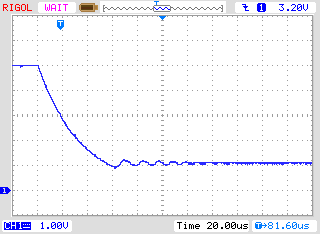
\includegraphics[width=8.3cm]{../PNG/AREF2_1V.png}
    \caption{from 5V to 1.1V }
    \label{pic:aref1}
  \end{subfigure}
  ~
  \begin{subfigure}[b]{8.6cm}
    \centering
    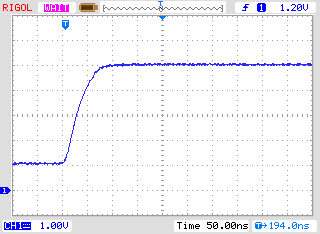
\includegraphics[width=8.3cm]{../PNG/AREF2VCC.png}
    \caption{from 1.1V to 5V}
    \label{pic:aref5}
  \end{subfigure}
  \caption{AREF switching with a \(1nF\) Capacitor}
\end{figure}


Additional parameters can be set in the files transistortester.h and config.h .
The file config.h contains global settings, defines the port / pin constellation,
 the clock frequency of the ADC and the resistor values used for measurement.
The file Transistortester.h contains the global variables and tables and also the text used for LCD output.
Normally there is no reason to change these values.


\chapter{Description of the measurement procedures}
\label{sec:measurement}
The simplified schematic of a Input/Output-Port pin of the ATmega is shown in figure~\ref{fig:port}.
The PUD switch isolates all ``pull up'' resistors of the ATmega. The output of a pin can be switched off
with the DD switch. The Input can operate regardless to the state of the switch DD.
The PORT switch usually defined the output level, but also switches the pull up resistor.
Because the Switches PORT and DD can not be changed at the same time but only one after another, the
pull up resistors can disturb the measurement. Therefore I prefere to disable the pull up resistors with the
PUD switch.
Of course all the switches are electronic type and the resistors \(19\Omega\) and \(22\Omega\) are approximated values.

\begin{figure}[H]
\centering

\includegraphics[]{../FIG/port.eps}
\caption{simplified diagram of each ATmega port pin}
\label{fig:port}
\end{figure}

Every of the three terminal probes of your Transistor Tester is build with three ATmega port pins,
which is shown as simplified diagram for the terminal probe TP2 (middle of three pins) in figure~\ref{fig:terminal}.

\begin{figure}[H]
\centering

\includegraphics[]{../FIG/terminal.eps}
\caption{simplified circuit of each measurement terminal probe TP}
\label{fig:terminal}
\end{figure}

Every test pin (measurement port) can be used as digital or analog input. This measurement capability is
independent of using the port as output.
Every test pin can be switched to output and in this mode it can be directly connected to GND (\(0V\)) or VCC (\(5V\)), 
or it can be connected via a \(680\Omega\) resistor or a \(470k\Omega\) resistor to either GND or VCC.
Table \ref{tab:case} shows all possible combination of measurements.
Notice, that the positive state can be switched directly to VCC (Port C) or it can be connected with the 
\(680\Omega\) resistor to VCC (Port B). The same possibility has the negative state of terminal probe to the GND side.
The test state means, that probe can be open (Input), connected with the \(470k\Omega\) resistor to VCC or GND,
or that the probe can be connected with the \(680\Omega\) resistor to VCC or GND.

\begin{table}[H]
  \begin{center}
    \begin{tabular}{| l | c | c | c |}
    \hline
      & state pin 1 & state pin 2 & state pin 3 \\
    \hline
   1. & positive    &  negative    &  test \\
   2. & positive    &  test       & negative \\
   3. & test        &  negative    & positive \\
   4. & test        &  positive    & negative \\
   5. & negative     &  test       & positive \\
   6. & negative     &  positive    &  test  \\
    \hline
    \end{tabular}
  \end{center}
  \caption{all combinations of measurement}
  \label{tab:case} 
\end{table}

If the capacitor measuring is configured for the tester, the tester will try to discharge the capacitors connected at all
test pins.
If discharge will fail, that means the remaining voltage is to high, the discharging will be aborted after about 12 seconds
with the meassage ''Cell!''. This can also be happen, if no capacitor is connected to any test pin.
The cause for this can be, that the cut-off voltage is choosed to low for this ATmega.
You can choose a higher voltage with the Makefile option CAP\_EMPTY\_LEVEL.


 %\newpage
\section{Measurement of Semiconductors}
The currentflow of the device with currentless control gate (third pin, also called Tristate pin)
is to be examined first.
The Tristate pin of the device under test is the base or gate for example.
One probe pin is selected as the positive side of the device and connected directly to VCC.
The other probe pin  selectes as negative side of the device.
The negative side is connected with the \(680\Omega\) resistor to GND.
With fieldeffect transistors the state of the device depends on the voltage of the gate.
The Tristate pin is first connected with the \(680\Omega\) resistor for 5ms to the GND side and
the voltage at the negative side is measured.
After that the voltage of the negative side is measured again during the Tristate pin switched
as input (High Impedance).
Then the assumed gate is connected with the \(680\Omega\) resistor for 5ms to the VCC side and
the voltage on the negative side is measured again.
If the measured voltage is lower than the first measurement result, this circuit will
be assumed as the right one. Then the voltage is measured again with currentless Tristate pin.

If the voltages of the negative pin with currentless Tristate pin and also with the 
fixed voltage of the Tristate pin is higher than 455mV, a depletion transistor type is assumed.
With the checking of both voltages we can avoid the wrong detection of some Germanium transistors with a higher
collector cutoff current as depletion transistors (JFET).

Then additional tests are done 
to differ N-channel JFET or N-D-MOSFET and P-channel JFET or P-D-MOSFET.
Die MOSFET-Versionen können erkannt werden durch das Fehlen von Steuerstrom in jedem
TriStatePins Zustand.
The MOSFET versions can be differed by the missing of gate current in any state
of the TriStatePin.

To get parameters of the depletion types, they will be measured with a \(680 \Omega\) resistor at
the source pin, as shown in figure \ref{fig:JFETcd} . This measurement will be done instead of the
usually measurement of current with the gate hold at source level, because
the \(I_\mathrm{DSS}\) current of the FET transistor can often not be reached
with the relative high resistance of the \(680 \Omega\) resistor.

\begin{figure}[H]
\centering

\includegraphics[]{../FIG/JFETcd.eps}
\caption{Measurement of the  Gate-Source voltage and Source current of a N-JFET transistor}
\label{fig:JFETcd}
\end{figure}

If the component has no current between positive probe and negative probe without signal at the
TristatePin, the next tests are specified in the next section \ref{sec:pnp}.
If current was detected, the next test is described in the diode section \ref{sec:diode}.

\subsection{Measurement of PNP Transistor or P-Channel-MOSFET}
\label{sec:pnp}
First the current amplification factor is measured with common collector (emitter follower) for the assumed
PNP transistor.
The measuring situation is shown in figure \ref{fig:pnpcc}.
If the measured voltage at the Base (\(UB\)) is above 9mV with the \(680\Omega\) resistor,
the hFE is build as \(hFE = \frac{UE-UB}{UB}\).
The voltage \(UE\) is the difference of the Emitter-voltage to VCC.
The difference between the \(22\Omega\) and \(19\Omega\) resistors are not respected.
If the \(UB\) voltage is below 10mV, the measurement is done with the \(470k\Omega\) resistor at the base.
In this case the current amplification factor is build as \(hFE = \frac{UE \cdot 470000}{UB \cdot (680+22)}\).

\begin{figure}[H]
\centering

\includegraphics[]{../FIG/PNPcc.eps}
\caption{hFE measurement of PNP transistor with common collector circuit }
\label{fig:pnpcc}
\end{figure}

Next the tests with common emitter are done for the assumed PNP transistor.
The positive side of component is now direct connected to VCC, the negative side \(680\Omega\) resistor
is connected to GND as shown in Figure \ref{fig:pnpce}. 
If the negative side of component has a voltage of above 3.4V, when the base side \(680\Omega\) resistor 
was connected to GND, it must be a PNP transistor or a P-Channel FET.
This can be easy find out by analysing the base voltage. If the base voltage is greater 0.97V, it must be a PNP.
For measuring the current amplification factor, the \(470k\Omega\) resistor is taken as Base resistor
instead of the \(680\Omega\).
The current amplification factor is build by \(hFE = \frac{(UC-UC0) \cdot 470000}{UB \cdot (680+19)}\) .
The voltage UC0 is the voltage at the colletor resistor without base current.
The higher current amplification factor is assumed to be the right one, this one or the one found with
the common collector circuit.


The values found for the PNP are only valid, if a second
set of measurements is done.
In order to prevent detecting the PNP in the inverse mode (collector and emitter are swapped),
the measurement with the higher current amplification is taken as the right one.
If base voltage is lower than 0.97V, it must be a P-E-MOS.
In this case the gate threshold voltage is measured
by switching the gate slowly with the \(470k\Omega\) resistor up and down, waiting for a digital
input signal change of the Drain side and then read the voltage of the gate pin.

\begin{figure}[H]
\centering

\includegraphics[]{../FIG/PNPce.eps}
\caption{test and hFE measurement of PNP transistor with common emitter circuit }
\label{fig:pnpce}
\end{figure}

\subsection{Measurement of NPN Transistor or N-Channel-MOSFET}
The measuring of NPN-Transistors begin in the same way as PNP-Transistors with measuring
the current amplification factor in the common collector circuit.
First measurement is done with a \(680\Omega\) base resistor switched to VCC. If the
voltage at the base resistor ist too low, the \(470k\Omega\) resistor is taken instead.
Measurement then continues with the common emitter circuit as shown in figure \ref{fig:npnce}.
\begin{figure}[H]
\centering

\includegraphics[]{../FIG/NPNce.eps}
\caption{test and hFE measurement of NPN transistor with common emitter circuit }
\label{fig:npnce}
\end{figure}
If the voltage of collector sinks below 1.6V, when the \(680\Omega\) base resistor is connected to VCC,
ist must be a NPN, N-Channel MOSFET or Thyristor/Triac.
With two simple tests a Thyristor or Triac can be identified.
If the gate pin resistor is connected for 10ms to GND and than made currentless, the current
at the anode should stay.
If then the anode resistor is short connected to GND and reconnected to VCC, the Thyristor should not
trigger again (no current).
Please keep in mind, that only low power Thyristors can be tested, because
the holding current of the tester can reach only 6mA.
If both tests attest a Thyristor, further tests with reverse polarity are done
to exclude or confirm a Triac.

If neither Thyristor nor Triac could be confirmed, it can be a NPN or N-Channel E-MOSFET.
The Base voltage of a NPN Transistor will be near the Emitter voltage, so this type can be
identified definitely.
The current amplification factor in the common emitter circuit is build by
\(hFE = \frac{(VCC-UC-UC0)\cdot 470000}{(VCC-UB)\cdot (680+22)}\).
If the voltage of the Base or better Gate  shows, that there is no or little current, part will be a N-Channel E-MOS 
(Enhancement MOSFET).
 In this case the threshold voltage is measured by switching the Gate slowly with
the \(470k\Omega\) resistor to VCC and GND, waiting for a digital input signal change of the Drain side and
then read the voltage of the Gate pin.
This measurement is done eleven times with ADC results accumulated as shown in Figure~\ref{fig:eleven}.
The result is multiplied by four and divided by 9 to get the voltage in mV resolution.
\begin{figure}[H]
\centering
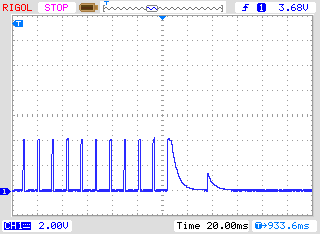
\includegraphics[]{../PNG/IRFU120gate.png}
\caption{measuring of threshold voltage of N-Channel-MOSFET}
\label{fig:eleven}
\end{figure}

\subsection{Simplified flowchart of the transistors tests}

\begin{figure}[H]
\centering

\includegraphics[]{../FIG/CheckSemi1.eps}
\caption{Flowchart transistor test Part 1, JFET and D-MOS}
\label{fig:ChkSemi1}
\end{figure}

\begin{figure}[H]
\centering

\includegraphics[]{../FIG/CheckSemi2.eps}
\caption{Flowchart transistor test Part 2, BJT and E-MOS}
\label{fig:ChkSemi2}
\end{figure}


\subsection{Measurement of Diodes}
\label{sec:diode}
If current is detected with the pre-tests, the behavior of the part will be checked to be a diode.
The flow voltage with the \(680\Omega\) resistor must be between 0.15V and 4.64V.
The flux voltage with the \(680\Omega\) must be greater than 1.125 times the flux voltage with
the \(470k\Omega\) resistor and sixteen times the flux voltage with the \(470k\Omega\) must be
greater than the flux voltage with the \(680\Omega\) resistor.
Additionally the afterward renewed measurement with the \(470k\Omega\) resistor should not have a higher voltage than
the previous measurement with the \(680\Omega\) resistor.
I hope, that this behavior identifies always a diode.
The identification of a diode by no current flow in the opposite direction is not
possible with a inverse parallel diode.
If only a single diode is detected, the residual current in reverse direction is measured with
the \(470k\Omega\) resistor at 5V. The resolution is about \(2nA\).
If the residual current is greater as \(5.3\mu A\) (voltage at
the \(470k\Omega\) is more than 2.5V), the measurement is done with the \(680\Omega\) instead.
Then the resolution is only about \(1\mu A\).
Furthermore  the capacity in reverse direction is also measured for single diodes.

\subsection{Results of different measurements}
The following three tables shows results of different test probes 
with one ATmega8, a ATmega168 and a ATmega328 processor.
The measurement of the inverse capacity value for the double diode MBR4045PT is 
only possible with cooling. This will be caused by high residual current of this 40A diode.
Also the capacity value of the inverse base emitter diode of the germanium transistor AC128 can
only be measured with cooling.

\begin{table}[H]
  \begin{center}
    \begin{tabular}{| l | c | c | c |}
    \hline
           & Mega8@8MHz & Mega168 @8MHz & Mega328 @8MHz \\
 Diode Type  &                  &                  &                  \\
    \hline
    \hline
1N4148     & Diode, 715mV,        & Diode, 718mV,            & Diode, 715mV,           \\
           &               1pF    &               0pF, 2nA   &               1pF, 4nA  \\
    \hline
1N4150     & Diode, 665mV,        & Diode, 672mV,            & Diode, 666V,           \\
           &               1pF    &               1pF, 4nA   &              2pF, 6nA  \\
    \hline
BA157      & Diode, 619mV,        & Diode, 621V,              & Diode, 615mV,            \\
           &               19pF   &              17pF, 12nA   &               18pF, 12nA \\
    \hline
BY398      & Diode, 538mV,        & Diode, 541mV,             & Diode, 537mV,            \\
           &               16pF   &               14pF, 63nA  &               15pF, 63nA \\
    \hline
1N4007     & Diode, 650mV,        & Diode, 655mV,            & Diode, 650mV,           \\
           &               13pF   &               10pF, 6nA  &               13pF, 6nA \\
    \hline
LED green  & Diode, 1.96V, 5pF    & Diode, 1.95V, 4pF   & Diode, 1.95V, 4pF \\
    \hline
ZPD2,7     & 2xDi, 743mV, 2.53V   & 2xDi, 737mV, 2.52V  & 2xDi, 733mV, 2.51V \\
    \hline
BU508A B+E & Diode, 609mV,        & Diode, 611mV,                & Diode, 606mV,              \\
           &               5.15nF &               5.20nF, 0.39uA &               5.25nF, 0.4uA\\
    \hline
BU508A B+C & Diode, 582mV,        & Diode, 586mV,             & Diode, 587mV,            \\
           &               256pF  &               255pF, 21nA &               259pF, 19nA\\
    \hline
AC128 B+E  & Diode, 272mV,        & Diode, 277mV,              & Diode, 273mV,             \\
           &               0pF    &               0pF, 2.2uA   &               0pF, 2.3uA  \\
    \hline
AC128 B+E  &                      &                     & Diode, 349mV,               \\
cooled     &                      &                     &               140pF, 0.57uA \\
    \hline
MBR20100CT & 2xDi, 337mV, 337mV   & 2xDi, 338mV, 338mV  & 2xDi, 336mV, 335mV  \\
    \hline
MBR20100CT & Diode, 337mV,        & Diode, 339mV,             & Diode, 337mV,            \\
           &               345pF  &               351pF, 29nA &               350pF, 25nA\\
    \hline
MBR4045PT  & Diode, 243mV,        & Diode, 233mV,               & Diode, 235mV,              \\
cooled     &               1.80nF &               1.94nF, 1.7uA &               1.95nF, 1.8uA\\
    \hline
SK14       & Diode,    mV,        & Diode,    mV,               & Diode, 263mV,              \\
           &                  0pF &                   pF,    nA &               0pF, 0.57uA\\
    \hline
SK14       & Diode,    mV,        & Diode,    mV,               & Diode, 334mV,              \\
cooled     &                   nF &                   pF,    nA &               88pF, 4nA\\
    \hline
SF38G      & Diode, 519mV,        & Diode, 521mV,            & Diode, 516mV,            \\
           &               107pF  &               105pF, 2nA &               106pF, 2nA \\
    \hline
    \end{tabular}
  \end{center}
  \caption{measurement results of diode testing}
  \label{tab:diodes} 
\end{table}

\begin{table}[H]
  \begin{center}
    \begin{tabular}{| l | c | c | c | c | c |}
    \hline
 Transistor & Typ & Mega8           & Mega328        & Mega328         & Mega328 \\
    Type     &     & common-         &                & common-         & common- \\
            &     & collector      &                & collector       & emitter \\
    \hline
    \hline
BU508A      & NPN & B=9, 601mV      &  B=9, 597mV    &   B=9, 598mV    & B=4, 484mV \\
    \hline
2N3055      & NPN & B=20, 557mV     &  B=21, 550mV   &   B=21, 550mV   & B=6, 442mV \\
    \hline
BC639       & NPN & B=148, 636mV    &  B=172, 629mV  &   B=172, 629mV  & B=158, 605mV \\
    \hline
BC640       & PNP & B=226, 650mV    &  B=176, 609mV  &   B=171, 655mV  & B=177, 608mV \\
    \hline
BC517       & NPN & B=23.9k, 1.23V  &  B=24.8k, 1.22V&   B=25.1k, 1.22V & B=764, 1.23V \\
    \hline
BC516       & PNP & B=75.9k, 1.21V  &  B=76.2k, 1.20V&   B=76.2k, 1.20V & B=760, 1.23V \\
    \hline
BC546B      & NPN & B=285, 694mV    &  B=427, 687mV  &   B=427, 687mV   & B=369, 683mV \\
    \hline
BC556B      & PNP & B=304, 704mV    &  B=254, 668mV  &   B=235, 709mV   & B=255, 668mV \\
    \hline
AC128 (Ge.) & PNP & B=63, 191mV     &  B=59, 191mV   &   B=57, 193mV    & B=43, 117mV \\
    \hline
BUL38D      & NPNp & B=37, 627mV    &  B=41, 617mV  &   B=40, 624mV     & B=36, 562mV \\
parasitic   & PNPn & B=11, 654mV    &  B=81, 543mV  &   B=10, 656mV     & B=83, 541mV \\
    \hline
BRY55/200   & Thyrist. &  0.84V     &  0.81V         &   0.81V          &  0.82V \\
    \hline
MAC97A6     & Triac    &  0.92V     &  0.90V         &   0.90V          &  0.90V \\
    \hline
    \end{tabular}
  \end{center}
  \caption{measurement results of bipolar transistor testing}
  \label{tab:bipolar} 
\end{table}

Some results are very different to the earlier results of the software of Markus Frejek.
For example a darlington transistor BC517 has been measured by the older software
with a hFE of 797 instead of 77200 and a base emitter voltage of 1438mV.
This will be caused by the additional measurement of current amplification with the
common collector circuit.
Also the new version shows the same low hFE result with the common emitter circiut,
as you can see in the last column of table \ref{tab:bipolar}.
The base emitter voltage is measured by the older Version as separate diode test with 1438mV.
Now the base emitter voltage is measured with the state of current amplification testing (1.20V).
The BUL38D Transistor has a build in protection diode over the anode and cathode of the NPN transistor,
by what a parasitical PNP transistor with swapped Base - Collector connection is build.
With software revision 1.10k both transistors are detected and marked
with a appended p.
The right transistor will be found with comparation of the gate - emitter junction capacitance.
It is assumed, that the right transistor has the higher junction capacitance.
If you hold down the start key during the output of the measurement result, the parameter of
the parasitical transistor are shown. With the label PNPn the existance of another transistor will be marked.
The parasitical transistor structure is build only by integration of the protection diode nearby
the transistor within the same material, not with a external diode.

The following table \ref{tab:germanium} shows the measurement results for germanium transistors, which are extra problematic
to measure because of the temperatur dependent and high residual collector current.
The results of the original version of Markus F. and the results of the actual 1.10k version are
compared together. The 1.10k version for a ATmega328 measures the current amplification factor with
common collector and common emitter circuit with respect to the collector residual current,
the higher result will be shown.
The collector residual current is not respected by earlier versions.

\begin{table}[H]
  \begin{center}
    \begin{tabular}{| l | c | c | c |}
    \hline
 Transistor & Mega8@1MHz          & Mega168 @8MHz       & Mega328 @8MHz    \\
    Type    & Original Version    & Version 1.10k       & Version 1.10k  \\
            & Markus F.           &                     &        \\
    \hline
    \hline
AC128       & PNP, B=52, 279mV    & PNP, B=59, 184mV    & PNP, B=59, 191mV    \\
    \hline
AC116-65    & PNP, B=505, 378mV   & PNP, B=72, 146mV    & PNP, B=72, 149mV    \\
    \hline
AC116-145   & PNP, B=485, 294mV   & PNP, B=146, 161mV    & PNP, B=146, 163mV   \\
    \hline
AC176-65    & NPN, B=98, 235mV    & NPN, B=58, 94mV    & NPN, B=56, 96mV     \\
    \hline
GC122       & PNP, B=84, 368mV    & PNP, B=55, 117mV    & PNP, B=56, 117mV    \\
    \hline
GC301       & PNP, B=48, 289mV    & PNP, B=39, 184mV    & PNP, B=39, 188mV    \\
    \hline
AD161       & NPN, B=360, 230mV   & NPN, B=296, 126mV   & NPN, B=298, 128mV    \\
    \hline
AD162       & PNP, B=2127, 280mV  & PNP, B=89, 107mV    & PNP, B=89, 107mV    \\
    \hline
    \end{tabular}
  \end{center}
  \caption{Measurement results of bipolar junction germanium transistors}
  \label{tab:germanium}
\end{table}

In the table \ref{tab:mos} the results of some field-effect transistor measurements are shown.
One measured parameters of the E-type MOS types is the gate-source voltage, by which the
digital input of the ATmega connected to the \(680\Omega\) drain resitor
changes the state.
The other parameter is the gate capacity value.
For very fast change of the gate voltage due to a small gate capacity, the detected voltage is
slightly inaccurate.
With the BS250 the Voltage changes from 2.6V to 2.5V, if you connect a additional
\(10nF\) capacitor to the gate-source.
For JFET transistors often the characteristic current Idss is specified,
the current in the drain when the gate-source voltage is 0V.
Here, however, the current is given by a \(680\Omega\) load resistance at the source side
of the JFET.
The load resistor generates a reverse voltage Vgs,
which is also shown.
Due to the symmetrical design of the JFET transistors, the drain and source can not be distinguished.


\begin{table}[H]
  \begin{center}
    \begin{tabular}{| l | c | c | c | c |}
    \hline
             &         & Mega8@8MHz       & Mega168 @8MHz    & Mega328 @8MHz \\
 Transistor  & Type    &                  &                  &               \\
    \hline
    \hline
ZVNL120A     & N-E-MOS & D, 1.6V, 147pF   & D, 1.5V,141pF    & D, 1.5V, 140pF \\
    \hline
IRF530N      & N-E-MOS & D, 3.6V, 1.55nF  & D, 3.6V, 1.54nF  & D, 3.6V, 1.54nF \\
    \hline
BS170        & N-E-MOS & D, 2.6V, 78pF    & D, 2.6V, 68pF    & D, 2.6V, 68pF \\
    \hline
IRL3803      & N-E-MOS & D, 2.3V, 9.81nF  & D, 2.3V, 9.71nF  & D, 2.3V, 9.74nF \\
    \hline
IRFU120N     & N-E-MOS & D, 4.2V, 909pF   & D, 4.2V, 913pF   & D, 4.2V, 911pF \\
    \hline
BUZ71A       & N-E-MOS & D, 3.2V, 714pF   & D, 3.2V, 708pF   & D, 3.2V, 705pF \\
    \hline
ZVP2106A     & P-E-MOS & D, 3.2V, 122pF   & D, 3.2V,115pF    & D, 3.2V, 116pF \\
    \hline
IRF5305      & P-E-MOS & D, 3.6V, 2.22nF  & D, 3.6V, 2.22nF  & D, 3.6V, 2.22nF \\
    \hline
BS250        & P-E-MOS & D, 2.6V, 53pF    & D, 2.6V, 43pF    & D, 2.6V, 44pF \\
    \hline
IRFU9024     & P-E-MOS & D, 3.5V, 937pF   & D, 3.6V, 945pF   & D, 3.5V, 933pF \\
    \hline
J310         & N-JFET  & 3.1mA Vgs=2.2V   & 3.1mA Vgs=2.2V   & 3.1mA Vgs=2.2V \\
Idss=24-60mA &         &                  &                  &              \\
    \hline
2N5459       & N-JFET  & 2.1mA Vgs=1.5V   & 2.1mA Vgs=1.5V   & 2.1mA Vgs=1.5V \\
Idss=4-16mA &          &                  &                  &              \\
    \hline
BF256C       & N-JFET  & 3.4mA Vgs=2.4V   & 3.4mA Vgs=2.4V   & 3.4mA Vgs=2.4V \\
Idss=11-18mA &         &                  &                  &              \\
    \hline
BF245A       & N-JFET  & 1.1mA Vgs=.75V   & 1.1mA Vgs=0.75V  & 1.1mA Vgs=0.75V \\
Idss=2-6mA   &         &                  &                  &              \\
    \hline
BF245B       & N-JFET  & 2.5mA Vgs=1.7V   & 2.5mA Vgs=1.7V   & 2.5mA Vgs=1.7V \\
Idss=6-15mA  &         &                  &                  &              \\
    \hline
BF245C       & N-JFET  & 3.9mA Vgs=2.7V   & 3.9mA Vgs=2.7V   & 3.9mA Vgs=2.7V \\
Idss=12-25mA &         &                  &                  &              \\
    \hline
J175        & P-JFET   & 3.2mA Vgs=2.2V   & 3.2mA Vgs=2.2V   & 3.2mA Vgs=2.2V \\
Idss=7-60mA &          &                  &                  &              \\
    \hline
2N5460      & P-JFET   & 0.78mA Vgs=0.54V & 0.77mA Vgs=0.54V & 0.78mA Vgs=0.54V \\
Idss=1-5mA  &          &                  &                  &              \\
    \hline
BSS139      & N-D-MOS  & 1.7mA Vgs=1.2V  & D, 1.7mA Vgs=1.2V & D, 1.7mA Vgs=1.2V \\
    \hline
BSS169      & N-D-MOS  & 2.6mA Vgs=1.8V  & D, 2.6mA Vgs=1.8V & D, 2.6mA Vgs=1.8V \\
    \hline
GP07N120    & N-E-IGBT & C=3.81nF Vt=4.2V & C=3.76nF Vt=4.2V & C=3.74nF Vt=4.2V \\
    \hline
    \end{tabular}
  \end{center}
  \caption{measurement results of MOS transistor testing}
  \label{tab:mos} 
\end{table}

 %\newpage
\section{Widerstands-Messung}
Jeder Widerstand wird mit vier verschiedenen Messmethoden in einer Stromrichtung vermessen.
Der gleiche Widerstand wird auch mit den gleichen vier Messmethoden in die andere Stromrichtung vermessen.
Die Messung in die Gegenrichtung wird nur für die Erkennung auf Widerstand benutzt.
Wenn die Abweichung dieser beiden Messungen zu groß ist, ist es kein Widerstand.

\subsection{Widerstandsmessung mit den 680-Ohm-Widerständen}
Die Messung des unbekannten Widerstandes Rx wird in zwei verschiedenen Wegen mit den \(680\Omega\)-Präzisionswiderständen
 durchgeführt.
Das Schaltbild dieser Messungen mit Testpin 1 (TP1) und Testpin 3 (TP3) werden vereinfacht in Abbildung~\ref{fig:RL1mes} und Abbildung~\ref{fig:RL2mes} als ein Beispiel von den sechs Kombinationsmöglichkeiten gezeigt.

\begin{figure}[H]
\centering

\includegraphics[]{../FIG/ResistormessL1.eps}
\caption{Messung Type 1 mit \(680\Omega\) }
\label{fig:RL1mes}
\end{figure}

\begin{figure}[H]
 \centering
 
\includegraphics[]{../FIG/ResistormessL2.eps}
 \caption{Messung Type 2 mit \(680\Omega\) }
\label{fig:RL2mes}
\end{figure}

Auf der linken Seite wird der Testpin 1 und auf der rechten Seite der Testpin 3 gezeigt.
In beiden Schaltungen kann man erkennen, dass der Anschluss 3 (TP3) mit VCC und die linke Seite (TP1) mit
GND verbunden ist.
Die Stromrichtung durch den Widerstand Rx ist immer die gleiche.
Die Werte für auf Ausgang geschaltete Ports werden mit roter Farbe dargestellt, 
die Werte für die Eingänge werden mit blauer Farbe dargestellt, inaktive Ports sind schwarz.
In beiden gezeigten Messmethoden sollte der Strom den gleichen Wert haben, weil die Summe der Widerstände zwischen
VCC und GND gleich ist, vorausgesetzt die eingebauten Widerstände sind gleich.
Normalerweise sind die gemessenen Spannungen aber nicht gleich, weil die Reihenfolge
der Widerstände vertauscht ist.

Das V-Symbol innerhalb eines Kreises markiert die Ports, die für die Spannungsmessung benutzt werden.
In beiden Konfigurationen kann der Wert des Widerstandes Rx aus den bekannten Widerstandswerten
und den gemessenen Spannungen berechnet werden, wenn das Verhältnis des Widerstands Rx und den \(680\Omega\)-Widerständen
 nicht zu hoch ist.
Der theoretische Spannungsverlauf wird in Abbildung~\ref{fig:RLvtot} gezeigt, wobei die Widerstandswerte 
in logarithmischer Skalierung dargestellt sind.
\begin{figure}[H]
\centering
% GNUPLOT: LaTeX picture with Postscript
\begingroup
  \makeatletter
  \providecommand\color[2][]{%
    \GenericError{(gnuplot) \space\space\space\@spaces}{%
      Package color not loaded in conjunction with
      terminal option `colourtext'%
    }{See the gnuplot documentation for explanation.%
    }{Either use 'blacktext' in gnuplot or load the package
      color.sty in LaTeX.}%
    \renewcommand\color[2][]{}%
  }%
  \providecommand\includegraphics[2][]{%
    \GenericError{(gnuplot) \space\space\space\@spaces}{%
      Package graphicx or graphics not loaded%
    }{See the gnuplot documentation for explanation.%
    }{The gnuplot epslatex terminal needs graphicx.sty or graphics.sty.}%
    \renewcommand\includegraphics[2][]{}%
  }%
  \providecommand\rotatebox[2]{#2}%
  \@ifundefined{ifGPcolor}{%
    \newif\ifGPcolor
    \GPcolortrue
  }{}%
  \@ifundefined{ifGPblacktext}{%
    \newif\ifGPblacktext
    \GPblacktexttrue
  }{}%
  % define a \g@addto@macro without @ in the name:
  \let\gplgaddtomacro\g@addto@macro
  % define empty templates for all commands taking text:
  \gdef\gplbacktext{}%
  \gdef\gplfronttext{}%
  \makeatother
  \ifGPblacktext
    % no textcolor at all
    \def\colorrgb#1{}%
    \def\colorgray#1{}%
  \else
    % gray or color?
    \ifGPcolor
      \def\colorrgb#1{\color[rgb]{#1}}%
      \def\colorgray#1{\color[gray]{#1}}%
      \expandafter\def\csname LTw\endcsname{\color{white}}%
      \expandafter\def\csname LTb\endcsname{\color{black}}%
      \expandafter\def\csname LTa\endcsname{\color{black}}%
      \expandafter\def\csname LT0\endcsname{\color[rgb]{1,0,0}}%
      \expandafter\def\csname LT1\endcsname{\color[rgb]{0,1,0}}%
      \expandafter\def\csname LT2\endcsname{\color[rgb]{0,0,1}}%
      \expandafter\def\csname LT3\endcsname{\color[rgb]{1,0,1}}%
      \expandafter\def\csname LT4\endcsname{\color[rgb]{0,1,1}}%
      \expandafter\def\csname LT5\endcsname{\color[rgb]{1,1,0}}%
      \expandafter\def\csname LT6\endcsname{\color[rgb]{0,0,0}}%
      \expandafter\def\csname LT7\endcsname{\color[rgb]{1,0.3,0}}%
      \expandafter\def\csname LT8\endcsname{\color[rgb]{0.5,0.5,0.5}}%
    \else
      % gray
      \def\colorrgb#1{\color{black}}%
      \def\colorgray#1{\color[gray]{#1}}%
      \expandafter\def\csname LTw\endcsname{\color{white}}%
      \expandafter\def\csname LTb\endcsname{\color{black}}%
      \expandafter\def\csname LTa\endcsname{\color{black}}%
      \expandafter\def\csname LT0\endcsname{\color{black}}%
      \expandafter\def\csname LT1\endcsname{\color{black}}%
      \expandafter\def\csname LT2\endcsname{\color{black}}%
      \expandafter\def\csname LT3\endcsname{\color{black}}%
      \expandafter\def\csname LT4\endcsname{\color{black}}%
      \expandafter\def\csname LT5\endcsname{\color{black}}%
      \expandafter\def\csname LT6\endcsname{\color{black}}%
      \expandafter\def\csname LT7\endcsname{\color{black}}%
      \expandafter\def\csname LT8\endcsname{\color{black}}%
    \fi
  \fi
  \setlength{\unitlength}{0.0500bp}%
  \begin{picture}(7200.00,5040.00)%
    \gplgaddtomacro\gplbacktext{%
      \csname LTb\endcsname%
      \put(1078,704){\makebox(0,0)[r]{\strut{} 0}}%
      \csname LTb\endcsname%
      \put(1078,1518){\makebox(0,0)[r]{\strut{} 1000}}%
      \csname LTb\endcsname%
      \put(1078,2332){\makebox(0,0)[r]{\strut{} 2000}}%
      \csname LTb\endcsname%
      \put(1078,3147){\makebox(0,0)[r]{\strut{} 3000}}%
      \csname LTb\endcsname%
      \put(1078,3961){\makebox(0,0)[r]{\strut{} 4000}}%
      \csname LTb\endcsname%
      \put(1078,4775){\makebox(0,0)[r]{\strut{} 5000}}%
      \csname LTb\endcsname%
      \put(1210,484){\makebox(0,0){\strut{}100m}}%
      \csname LTb\endcsname%
      \put(2142,484){\makebox(0,0){\strut{}1 }}%
      \csname LTb\endcsname%
      \put(3074,484){\makebox(0,0){\strut{}10 }}%
      \csname LTb\endcsname%
      \put(4007,484){\makebox(0,0){\strut{}100 }}%
      \csname LTb\endcsname%
      \put(4939,484){\makebox(0,0){\strut{}1k}}%
      \csname LTb\endcsname%
      \put(5871,484){\makebox(0,0){\strut{}10k}}%
      \csname LTb\endcsname%
      \put(6803,484){\makebox(0,0){\strut{}100k}}%
      \put(176,2739){\rotatebox{-270}{\makebox(0,0){\strut{}voltage / mV}}}%
      \put(4006,154){\makebox(0,0){\strut{}resistor Rx / Ohm}}%
      \put(4006,4665){\makebox(0,0){\strut{}}}%
      \put(286,110){\makebox(0,0)[l]{\strut{}}}%
    }%
    \gplgaddtomacro\gplfronttext{%
      \csname LTb\endcsname%
      \put(3594,3094){\makebox(0,0)[r]{\strut{}PC2, type 1}}%
      \csname LTb\endcsname%
      \put(3594,2874){\makebox(0,0)[r]{\strut{}PC0, type 2}}%
    }%
    \gplbacktext
    \put(0,0){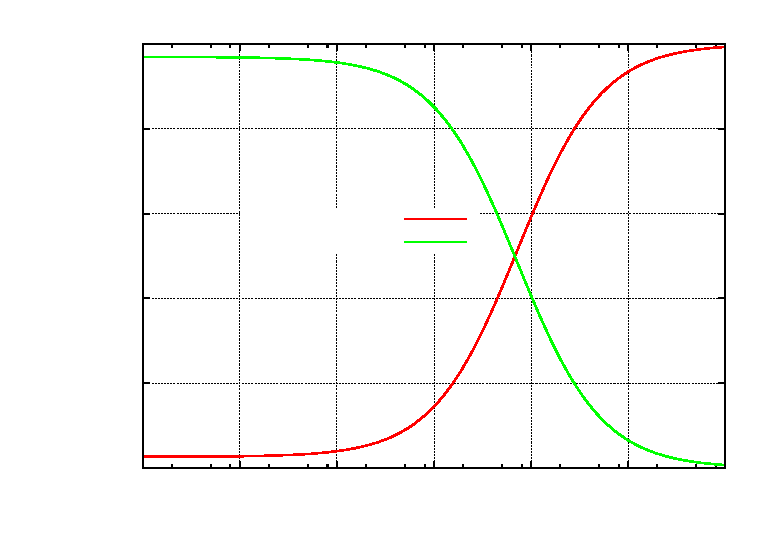
\includegraphics{../GNU/RLvtot}}%
    \gplfronttext
  \end{picture}%
\endgroup

\caption{Spannung von Type 1 und Type 2 mit Messwiderstand \(680\Omega\) }
\label{fig:RLvtot}
\end{figure}
Die Verlauf für Messung Type 1 wird in Abbildung~\ref{fig:RLvlow} mit gespreizter Darstellung für die unteren Widerstandwerte gezeigt.
Wie man sehen kann, braucht man eine bessere ADC-Auflösung als die möglichen \(4,9mV\) bei der \(5V\) ADC-Referenz, um richtige
Widerstandswerte von der gemessenen Spannung unter \(2\Omega\) zu erhalten.
Es gibt nur drei ADC-Stufen mit der \(5V\)-Referenz zwischen \(0\Omega\) und \(2\Omega\).
Hier kann die Bereichsumschaltung mit der AUTOSCALE\_ADC-Option helfen.
Der gleiche gespreizte Bereich für die Type-2-Messung wird in Abbildung~\ref{fig:RLvhigh} gezeigt.
Unglücklicherweise kann man nicht die höhere ADC-Auflösung für Messmethode Type 2 benutzen,
weil die Spannung zu hoch ist und unser ATmega keine differentiellen ADC-Eingänge besitzt.
Die Messungen mit den \(680\Omega\)-Widerständen werden bis zu einem Widerstandswert von 
\(20k\Omega\) (Spannung ist unter \(169mV\)) zur Bestimmung des Messergebnisses verwendet.

Für höhere Widerstandswerte werden Messungen mit den \(470k\Omega\)-Widerständen benutzt.
Der Mittelwert von beiden Messungen wird für den angezeigten Widerstandwert benutzt, wenn alle Messungen ergeben,
dass es kein anderes Bauteil ist.
Wenn die AUTOSCALE\_ADC-Funktion benutzt wird und eine der gemessenen Spannungen für beide Versionen unter 0,98V liegt,
wird ein gewichteter Mittelwert mit Faktor Vier für die Messung mit der Spannung unter \(0,98V\) benutzt. Der andere Wert wird mit Faktor Eins bewertet.
Das wird wegen der Faktor Vier besseren Auflösung dieser Messung gemacht.
Faktor Vier wird nur für ATmega168- und ATmega328-Prozessoren verwendet, für ATmega8 wird ein
Faktor Zwei als Wichtung benutzt wenn die Spannung unter \(0,98V\) ist, weil die ADC-Referenzspannung hier \(2,56V\) statt \(1,1V\) beträgt.
Wenn der ATmega mehr als 8 KByte Flashspeicher besitzt, wird die Spannungsmessung an den Widerständen so lange verzögert,
bis keine Änderung mehr festgestellt wird oder eine Zeitgrenze überschritten wird.
Durch diese Maßnahme werden auch große Kondensatoren nicht mehr irrtümlich als
Widerstände erkannt und der Gleichstrom-Widerstand großer Induktivitäten wird richtig gemessen.

\begin{figure}[H]
  \begin{subfigure}[b]{9cm}
    \centering
    \resizebox{9cm}{!}{% GNUPLOT: LaTeX picture with Postscript
\begingroup
  \makeatletter
  \providecommand\color[2][]{%
    \GenericError{(gnuplot) \space\space\space\@spaces}{%
      Package color not loaded in conjunction with
      terminal option `colourtext'%
    }{See the gnuplot documentation for explanation.%
    }{Either use 'blacktext' in gnuplot or load the package
      color.sty in LaTeX.}%
    \renewcommand\color[2][]{}%
  }%
  \providecommand\includegraphics[2][]{%
    \GenericError{(gnuplot) \space\space\space\@spaces}{%
      Package graphicx or graphics not loaded%
    }{See the gnuplot documentation for explanation.%
    }{The gnuplot epslatex terminal needs graphicx.sty or graphics.sty.}%
    \renewcommand\includegraphics[2][]{}%
  }%
  \providecommand\rotatebox[2]{#2}%
  \@ifundefined{ifGPcolor}{%
    \newif\ifGPcolor
    \GPcolortrue
  }{}%
  \@ifundefined{ifGPblacktext}{%
    \newif\ifGPblacktext
    \GPblacktexttrue
  }{}%
  % define a \g@addto@macro without @ in the name:
  \let\gplgaddtomacro\g@addto@macro
  % define empty templates for all commands taking text:
  \gdef\gplbacktext{}%
  \gdef\gplfronttext{}%
  \makeatother
  \ifGPblacktext
    % no textcolor at all
    \def\colorrgb#1{}%
    \def\colorgray#1{}%
  \else
    % gray or color?
    \ifGPcolor
      \def\colorrgb#1{\color[rgb]{#1}}%
      \def\colorgray#1{\color[gray]{#1}}%
      \expandafter\def\csname LTw\endcsname{\color{white}}%
      \expandafter\def\csname LTb\endcsname{\color{black}}%
      \expandafter\def\csname LTa\endcsname{\color{black}}%
      \expandafter\def\csname LT0\endcsname{\color[rgb]{1,0,0}}%
      \expandafter\def\csname LT1\endcsname{\color[rgb]{0,1,0}}%
      \expandafter\def\csname LT2\endcsname{\color[rgb]{0,0,1}}%
      \expandafter\def\csname LT3\endcsname{\color[rgb]{1,0,1}}%
      \expandafter\def\csname LT4\endcsname{\color[rgb]{0,1,1}}%
      \expandafter\def\csname LT5\endcsname{\color[rgb]{1,1,0}}%
      \expandafter\def\csname LT6\endcsname{\color[rgb]{0,0,0}}%
      \expandafter\def\csname LT7\endcsname{\color[rgb]{1,0.3,0}}%
      \expandafter\def\csname LT8\endcsname{\color[rgb]{0.5,0.5,0.5}}%
    \else
      % gray
      \def\colorrgb#1{\color{black}}%
      \def\colorgray#1{\color[gray]{#1}}%
      \expandafter\def\csname LTw\endcsname{\color{white}}%
      \expandafter\def\csname LTb\endcsname{\color{black}}%
      \expandafter\def\csname LTa\endcsname{\color{black}}%
      \expandafter\def\csname LT0\endcsname{\color{black}}%
      \expandafter\def\csname LT1\endcsname{\color{black}}%
      \expandafter\def\csname LT2\endcsname{\color{black}}%
      \expandafter\def\csname LT3\endcsname{\color{black}}%
      \expandafter\def\csname LT4\endcsname{\color{black}}%
      \expandafter\def\csname LT5\endcsname{\color{black}}%
      \expandafter\def\csname LT6\endcsname{\color{black}}%
      \expandafter\def\csname LT7\endcsname{\color{black}}%
      \expandafter\def\csname LT8\endcsname{\color{black}}%
    \fi
  \fi
  \setlength{\unitlength}{0.0500bp}%
  \begin{picture}(7200.00,5040.00)%
    \gplgaddtomacro\gplbacktext{%
      \csname LTb\endcsname%
      \put(946,704){\makebox(0,0)[r]{\strut{} 130}}%
      \csname LTb\endcsname%
      \put(946,995){\makebox(0,0)[r]{\strut{} 135}}%
      \csname LTb\endcsname%
      \put(946,1286){\makebox(0,0)[r]{\strut{} 140}}%
      \csname LTb\endcsname%
      \put(946,1576){\makebox(0,0)[r]{\strut{} 145}}%
      \csname LTb\endcsname%
      \put(946,1867){\makebox(0,0)[r]{\strut{} 150}}%
      \csname LTb\endcsname%
      \put(946,2158){\makebox(0,0)[r]{\strut{} 155}}%
      \csname LTb\endcsname%
      \put(946,2449){\makebox(0,0)[r]{\strut{} 160}}%
      \csname LTb\endcsname%
      \put(946,2740){\makebox(0,0)[r]{\strut{} 165}}%
      \csname LTb\endcsname%
      \put(946,3030){\makebox(0,0)[r]{\strut{} 170}}%
      \csname LTb\endcsname%
      \put(946,3321){\makebox(0,0)[r]{\strut{} 175}}%
      \csname LTb\endcsname%
      \put(946,3612){\makebox(0,0)[r]{\strut{} 180}}%
      \csname LTb\endcsname%
      \put(946,3903){\makebox(0,0)[r]{\strut{} 185}}%
      \csname LTb\endcsname%
      \put(946,4193){\makebox(0,0)[r]{\strut{} 190}}%
      \csname LTb\endcsname%
      \put(946,4484){\makebox(0,0)[r]{\strut{} 195}}%
      \csname LTb\endcsname%
      \put(946,4775){\makebox(0,0)[r]{\strut{} 200}}%
      \csname LTb\endcsname%
      \put(1078,484){\makebox(0,0){\strut{} 0}}%
      \csname LTb\endcsname%
      \put(1651,484){\makebox(0,0){\strut{} 1}}%
      \csname LTb\endcsname%
      \put(2223,484){\makebox(0,0){\strut{} 2}}%
      \csname LTb\endcsname%
      \put(2796,484){\makebox(0,0){\strut{} 3}}%
      \csname LTb\endcsname%
      \put(3368,484){\makebox(0,0){\strut{} 4}}%
      \csname LTb\endcsname%
      \put(3941,484){\makebox(0,0){\strut{} 5}}%
      \csname LTb\endcsname%
      \put(4513,484){\makebox(0,0){\strut{} 6}}%
      \csname LTb\endcsname%
      \put(5086,484){\makebox(0,0){\strut{} 7}}%
      \csname LTb\endcsname%
      \put(5658,484){\makebox(0,0){\strut{} 8}}%
      \csname LTb\endcsname%
      \put(6231,484){\makebox(0,0){\strut{} 9}}%
      \csname LTb\endcsname%
      \put(6803,484){\makebox(0,0){\strut{} 10}}%
      \put(176,2739){\rotatebox{-270}{\makebox(0,0){\strut{}voltage / mV}}}%
      \put(3940,154){\makebox(0,0){\strut{}resistor Rx / Ohm}}%
      \put(3940,4665){\makebox(0,0){\strut{}}}%
    }%
    \gplgaddtomacro\gplfronttext{%
      \csname LTb\endcsname%
      \put(5816,4602){\makebox(0,0)[r]{\strut{}PC2, type 1}}%
    }%
    \gplbacktext
    \put(0,0){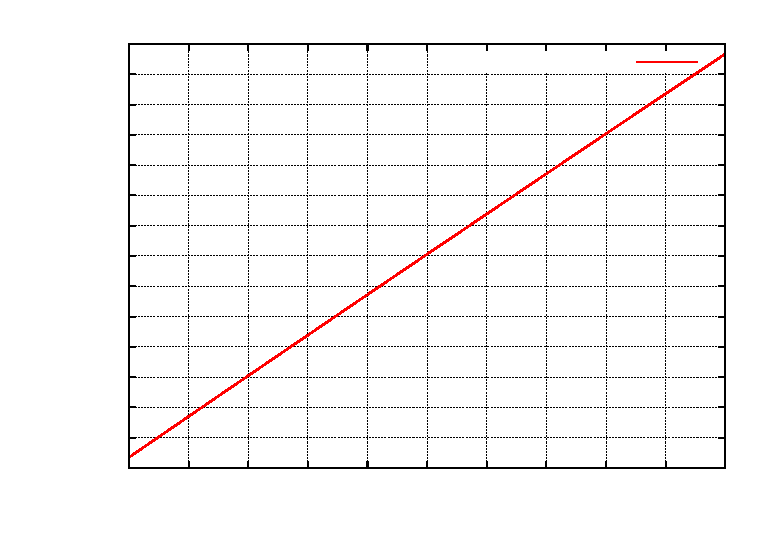
\includegraphics{../GNU/RLvlow}}%
    \gplfronttext
  \end{picture}%
\endgroup
}
    \caption{Type 1 Messung}
    \label{fig:RLvlow}
  \end{subfigure}
  ~
  \begin{subfigure}[b]{9cm}
    \centering
    \resizebox{9cm}{!}{% GNUPLOT: LaTeX picture with Postscript
\begingroup
  \makeatletter
  \providecommand\color[2][]{%
    \GenericError{(gnuplot) \space\space\space\@spaces}{%
      Package color not loaded in conjunction with
      terminal option `colourtext'%
    }{See the gnuplot documentation for explanation.%
    }{Either use 'blacktext' in gnuplot or load the package
      color.sty in LaTeX.}%
    \renewcommand\color[2][]{}%
  }%
  \providecommand\includegraphics[2][]{%
    \GenericError{(gnuplot) \space\space\space\@spaces}{%
      Package graphicx or graphics not loaded%
    }{See the gnuplot documentation for explanation.%
    }{The gnuplot epslatex terminal needs graphicx.sty or graphics.sty.}%
    \renewcommand\includegraphics[2][]{}%
  }%
  \providecommand\rotatebox[2]{#2}%
  \@ifundefined{ifGPcolor}{%
    \newif\ifGPcolor
    \GPcolortrue
  }{}%
  \@ifundefined{ifGPblacktext}{%
    \newif\ifGPblacktext
    \GPblacktexttrue
  }{}%
  % define a \g@addto@macro without @ in the name:
  \let\gplgaddtomacro\g@addto@macro
  % define empty templates for all commands taking text:
  \gdef\gplbacktext{}%
  \gdef\gplfronttext{}%
  \makeatother
  \ifGPblacktext
    % no textcolor at all
    \def\colorrgb#1{}%
    \def\colorgray#1{}%
  \else
    % gray or color?
    \ifGPcolor
      \def\colorrgb#1{\color[rgb]{#1}}%
      \def\colorgray#1{\color[gray]{#1}}%
      \expandafter\def\csname LTw\endcsname{\color{white}}%
      \expandafter\def\csname LTb\endcsname{\color{black}}%
      \expandafter\def\csname LTa\endcsname{\color{black}}%
      \expandafter\def\csname LT0\endcsname{\color[rgb]{1,0,0}}%
      \expandafter\def\csname LT1\endcsname{\color[rgb]{0,1,0}}%
      \expandafter\def\csname LT2\endcsname{\color[rgb]{0,0,1}}%
      \expandafter\def\csname LT3\endcsname{\color[rgb]{1,0,1}}%
      \expandafter\def\csname LT4\endcsname{\color[rgb]{0,1,1}}%
      \expandafter\def\csname LT5\endcsname{\color[rgb]{1,1,0}}%
      \expandafter\def\csname LT6\endcsname{\color[rgb]{0,0,0}}%
      \expandafter\def\csname LT7\endcsname{\color[rgb]{1,0.3,0}}%
      \expandafter\def\csname LT8\endcsname{\color[rgb]{0.5,0.5,0.5}}%
    \else
      % gray
      \def\colorrgb#1{\color{black}}%
      \def\colorgray#1{\color[gray]{#1}}%
      \expandafter\def\csname LTw\endcsname{\color{white}}%
      \expandafter\def\csname LTb\endcsname{\color{black}}%
      \expandafter\def\csname LTa\endcsname{\color{black}}%
      \expandafter\def\csname LT0\endcsname{\color{black}}%
      \expandafter\def\csname LT1\endcsname{\color{black}}%
      \expandafter\def\csname LT2\endcsname{\color{black}}%
      \expandafter\def\csname LT3\endcsname{\color{black}}%
      \expandafter\def\csname LT4\endcsname{\color{black}}%
      \expandafter\def\csname LT5\endcsname{\color{black}}%
      \expandafter\def\csname LT6\endcsname{\color{black}}%
      \expandafter\def\csname LT7\endcsname{\color{black}}%
      \expandafter\def\csname LT8\endcsname{\color{black}}%
    \fi
  \fi
  \setlength{\unitlength}{0.0500bp}%
  \begin{picture}(7200.00,5040.00)%
    \gplgaddtomacro\gplbacktext{%
      \csname LTb\endcsname%
      \put(1078,704){\makebox(0,0)[r]{\strut{} 4780}}%
      \csname LTb\endcsname%
      \put(1078,995){\makebox(0,0)[r]{\strut{} 4785}}%
      \csname LTb\endcsname%
      \put(1078,1286){\makebox(0,0)[r]{\strut{} 4790}}%
      \csname LTb\endcsname%
      \put(1078,1576){\makebox(0,0)[r]{\strut{} 4795}}%
      \csname LTb\endcsname%
      \put(1078,1867){\makebox(0,0)[r]{\strut{} 4800}}%
      \csname LTb\endcsname%
      \put(1078,2158){\makebox(0,0)[r]{\strut{} 4805}}%
      \csname LTb\endcsname%
      \put(1078,2449){\makebox(0,0)[r]{\strut{} 4810}}%
      \csname LTb\endcsname%
      \put(1078,2740){\makebox(0,0)[r]{\strut{} 4815}}%
      \csname LTb\endcsname%
      \put(1078,3030){\makebox(0,0)[r]{\strut{} 4820}}%
      \csname LTb\endcsname%
      \put(1078,3321){\makebox(0,0)[r]{\strut{} 4825}}%
      \csname LTb\endcsname%
      \put(1078,3612){\makebox(0,0)[r]{\strut{} 4830}}%
      \csname LTb\endcsname%
      \put(1078,3903){\makebox(0,0)[r]{\strut{} 4835}}%
      \csname LTb\endcsname%
      \put(1078,4193){\makebox(0,0)[r]{\strut{} 4840}}%
      \csname LTb\endcsname%
      \put(1078,4484){\makebox(0,0)[r]{\strut{} 4845}}%
      \csname LTb\endcsname%
      \put(1078,4775){\makebox(0,0)[r]{\strut{} 4850}}%
      \csname LTb\endcsname%
      \put(1210,484){\makebox(0,0){\strut{} 0}}%
      \csname LTb\endcsname%
      \put(1769,484){\makebox(0,0){\strut{} 1}}%
      \csname LTb\endcsname%
      \put(2329,484){\makebox(0,0){\strut{} 2}}%
      \csname LTb\endcsname%
      \put(2888,484){\makebox(0,0){\strut{} 3}}%
      \csname LTb\endcsname%
      \put(3447,484){\makebox(0,0){\strut{} 4}}%
      \csname LTb\endcsname%
      \put(4007,484){\makebox(0,0){\strut{} 5}}%
      \csname LTb\endcsname%
      \put(4566,484){\makebox(0,0){\strut{} 6}}%
      \csname LTb\endcsname%
      \put(5125,484){\makebox(0,0){\strut{} 7}}%
      \csname LTb\endcsname%
      \put(5684,484){\makebox(0,0){\strut{} 8}}%
      \csname LTb\endcsname%
      \put(6244,484){\makebox(0,0){\strut{} 9}}%
      \csname LTb\endcsname%
      \put(6803,484){\makebox(0,0){\strut{} 10}}%
      \put(176,2739){\rotatebox{-270}{\makebox(0,0){\strut{}voltage / mV}}}%
      \put(4006,154){\makebox(0,0){\strut{}resistor Rx / Ohm}}%
      \put(4006,4665){\makebox(0,0){\strut{}}}%
      \put(286,110){\makebox(0,0)[l]{\strut{}}}%
    }%
    \gplgaddtomacro\gplfronttext{%
      \csname LTb\endcsname%
      \put(5816,4602){\makebox(0,0)[r]{\strut{}PC0, type 2}}%
    }%
    \gplbacktext
    \put(0,0){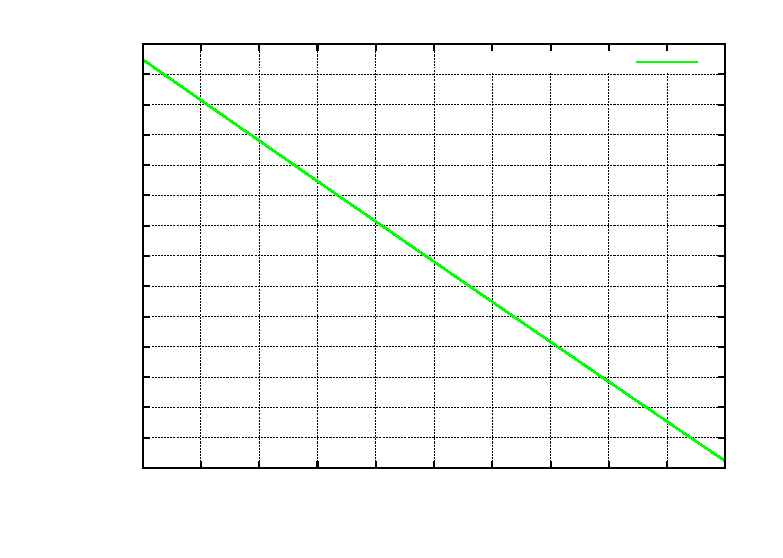
\includegraphics{../GNU/RLvhigh}}%
    \gplfronttext
  \end{picture}%
\endgroup
}
    \caption{Type 2 Messung}
    \label{fig:RLvhigh}
  \end{subfigure}
  \caption{Ausschnitt des theoretischen Spannungsverlauf von \(0\Omega\) bis \(10\Omega\)}
\end{figure}


\subsection{Widerstandsmessung mit den 470-kOhm-Widerständen}
Die nächsten Abbildungen~\ref{fig:RH1mes} und \ref{fig:RH2mes} zeigen die gleichen Messmethoden für die Messungen mit
 \(470k\Omega\)-Präzisionswiderständen.
Weil \(470k\Omega\) in Relation zu den Port-Widerständen \(22\Omega\) und \(19\Omega\) sehr groß ist,
können die Port-Widerstände für die Berechnung des Widerstandswertes Rx vernachlässigt werden.

Für beide Messmethoden mit den \(470k\Omega\)-Widerständen wird nur eine Spannung gemessen, weil der Strom
so niedrig ist, dass keine Spannungsdifferenz an den internen Port Widerständen gemessen werden kann (wie zu erwarten).
Der theoretische Spannungsverlauf wird in Abbildung~\ref{fig:RHv} gezeigt, wobei die Widerstandswerte wieder in
logarithmischer Skalierung gezeigt werden.
Der theoretische Verlauf in diesem Diagramm endet bei \(100M\Omega\), aber das Ergebnis des Testers wird auf
 \(60M\Omega\) begrenzt, anderenfalls nimmt der Tester an, dass kein Widerstand angeschlossen ist.
Als Ergebnis wird der gewichtete Mittelwert von beiden Messmethoden verwendet. Dies geschieht nach den gleichen Regeln, die schon bei
den Messungen mit den  \(680\Omega\) Widerständen beschrieben wurden.
Ich habe beobachtet, dass die Messergebnisse für alle ATmega-Typen  näher am wahren Wert liegen, wenn zum Messergebnis
ein konstanter Offset von \(350\Omega\) addiert wird.
Dieser Offset kann mit der Konstante RH\_OFFSET (define) in der Datei config.h angepasst werden.

\begin{figure}[H]
\centering

\includegraphics[]{../FIG/ResistormessH1.eps}
\caption{Messung Type 3 mit \(470k\Omega\) }
\label{fig:RH1mes}
\end{figure}

\begin{figure}[H]
 \centering
 
\includegraphics[]{../FIG/ResistormessH2.eps}
 \caption{Messung Type 4 mit \(470k\Omega\) }
\label{fig:RH2mes}
\end{figure}

\begin{figure}[H]
\centering
% GNUPLOT: LaTeX picture with Postscript
\begingroup
  \makeatletter
  \providecommand\color[2][]{%
    \GenericError{(gnuplot) \space\space\space\@spaces}{%
      Package color not loaded in conjunction with
      terminal option `colourtext'%
    }{See the gnuplot documentation for explanation.%
    }{Either use 'blacktext' in gnuplot or load the package
      color.sty in LaTeX.}%
    \renewcommand\color[2][]{}%
  }%
  \providecommand\includegraphics[2][]{%
    \GenericError{(gnuplot) \space\space\space\@spaces}{%
      Package graphicx or graphics not loaded%
    }{See the gnuplot documentation for explanation.%
    }{The gnuplot epslatex terminal needs graphicx.sty or graphics.sty.}%
    \renewcommand\includegraphics[2][]{}%
  }%
  \providecommand\rotatebox[2]{#2}%
  \@ifundefined{ifGPcolor}{%
    \newif\ifGPcolor
    \GPcolortrue
  }{}%
  \@ifundefined{ifGPblacktext}{%
    \newif\ifGPblacktext
    \GPblacktexttrue
  }{}%
  % define a \g@addto@macro without @ in the name:
  \let\gplgaddtomacro\g@addto@macro
  % define empty templates for all commands taking text:
  \gdef\gplbacktext{}%
  \gdef\gplfronttext{}%
  \makeatother
  \ifGPblacktext
    % no textcolor at all
    \def\colorrgb#1{}%
    \def\colorgray#1{}%
  \else
    % gray or color?
    \ifGPcolor
      \def\colorrgb#1{\color[rgb]{#1}}%
      \def\colorgray#1{\color[gray]{#1}}%
      \expandafter\def\csname LTw\endcsname{\color{white}}%
      \expandafter\def\csname LTb\endcsname{\color{black}}%
      \expandafter\def\csname LTa\endcsname{\color{black}}%
      \expandafter\def\csname LT0\endcsname{\color[rgb]{1,0,0}}%
      \expandafter\def\csname LT1\endcsname{\color[rgb]{0,1,0}}%
      \expandafter\def\csname LT2\endcsname{\color[rgb]{0,0,1}}%
      \expandafter\def\csname LT3\endcsname{\color[rgb]{1,0,1}}%
      \expandafter\def\csname LT4\endcsname{\color[rgb]{0,1,1}}%
      \expandafter\def\csname LT5\endcsname{\color[rgb]{1,1,0}}%
      \expandafter\def\csname LT6\endcsname{\color[rgb]{0,0,0}}%
      \expandafter\def\csname LT7\endcsname{\color[rgb]{1,0.3,0}}%
      \expandafter\def\csname LT8\endcsname{\color[rgb]{0.5,0.5,0.5}}%
    \else
      % gray
      \def\colorrgb#1{\color{black}}%
      \def\colorgray#1{\color[gray]{#1}}%
      \expandafter\def\csname LTw\endcsname{\color{white}}%
      \expandafter\def\csname LTb\endcsname{\color{black}}%
      \expandafter\def\csname LTa\endcsname{\color{black}}%
      \expandafter\def\csname LT0\endcsname{\color{black}}%
      \expandafter\def\csname LT1\endcsname{\color{black}}%
      \expandafter\def\csname LT2\endcsname{\color{black}}%
      \expandafter\def\csname LT3\endcsname{\color{black}}%
      \expandafter\def\csname LT4\endcsname{\color{black}}%
      \expandafter\def\csname LT5\endcsname{\color{black}}%
      \expandafter\def\csname LT6\endcsname{\color{black}}%
      \expandafter\def\csname LT7\endcsname{\color{black}}%
      \expandafter\def\csname LT8\endcsname{\color{black}}%
    \fi
  \fi
  \setlength{\unitlength}{0.0500bp}%
  \begin{picture}(7200.00,5040.00)%
    \gplgaddtomacro\gplbacktext{%
      \csname LTb\endcsname%
      \put(1078,704){\makebox(0,0)[r]{\strut{} 0}}%
      \csname LTb\endcsname%
      \put(1078,1518){\makebox(0,0)[r]{\strut{} 1000}}%
      \csname LTb\endcsname%
      \put(1078,2332){\makebox(0,0)[r]{\strut{} 2000}}%
      \csname LTb\endcsname%
      \put(1078,3147){\makebox(0,0)[r]{\strut{} 3000}}%
      \csname LTb\endcsname%
      \put(1078,3961){\makebox(0,0)[r]{\strut{} 4000}}%
      \csname LTb\endcsname%
      \put(1078,4775){\makebox(0,0)[r]{\strut{} 5000}}%
      \csname LTb\endcsname%
      \put(1210,484){\makebox(0,0){\strut{}10k}}%
      \csname LTb\endcsname%
      \put(2608,484){\makebox(0,0){\strut{}100k}}%
      \csname LTb\endcsname%
      \put(4007,484){\makebox(0,0){\strut{}1M}}%
      \csname LTb\endcsname%
      \put(5405,484){\makebox(0,0){\strut{}10M}}%
      \csname LTb\endcsname%
      \put(6803,484){\makebox(0,0){\strut{}100M}}%
      \put(176,2739){\rotatebox{-270}{\makebox(0,0){\strut{}voltage / mV}}}%
      \put(4006,154){\makebox(0,0){\strut{}resistor Rx / Ohm}}%
      \put(4006,4665){\makebox(0,0){\strut{}}}%
    }%
    \gplgaddtomacro\gplfronttext{%
      \csname LTb\endcsname%
      \put(5948,2874){\makebox(0,0)[r]{\strut{}PC2 type 3}}%
      \csname LTb\endcsname%
      \put(5948,2654){\makebox(0,0)[r]{\strut{}PC0, type 4}}%
    }%
    \gplbacktext
    \put(0,0){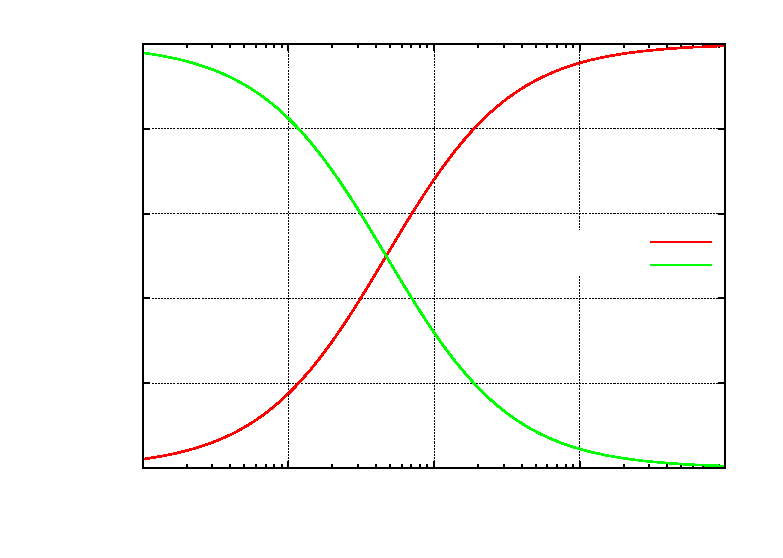
\includegraphics{../GNU/RHv}}%
    \gplfronttext
  \end{picture}%
\endgroup

\caption{Spannungen bei Messungen von Type 3 und Type 4  mit \(470k\Omega\) }
\label{fig:RHv}
\end{figure}

\subsection{Ergebnisse der Widerstands-Messung}
Abbildung~\ref{fig:mega8res} zeigt den relativen Fehler der Widerstandmessung mit drei verschiedenen ATmega8. 
Zusätzlich werden die Messergebnisse einiger Widerstände mit der Originalsoftware von Markus F. als
,,Mega8orig'' gezeigt.
Die Messergebnisse der gleichen Widerstände mit je drei ATmega8A und drei ATmega8L werden in den Abbildungen
\ref{fig:mega8Ares} und \ref{fig:mega8Lres} gezeigt.
Abbildung~\ref{fig:mega168res} zeigt die gleichen Messungen mit einem ATmega168.
,,Mega168'' sind die Ergebnisse ohne die AUTOSCALE\_ADC Option, ,,Mega168as'' die mit der
 AUTOSCALE\_ADC-Option.

Mit dem ATmega168 scheint es möglich zu sein, Messungen von Widerständen im
Bereich von \(20\Omega\) bis \(20M\Omega\) mit einem Messfehler von unter \(\pm1\%\) durchzuführen.
Für Messungen unterhalb von \(100\Omega\) sollte man berücksichtigen, dass jede Prüfklemme mit Kabel ebenfalls
einen Widerstandwert hat.
Es ist besser, den Widerstand direkt mit den Anschlussklemmen zu verbinden.
Wenn das nicht möglich ist, sollte man der Widerstandswert der kurzgeschlossenen Prüfklemmen vom Messergebnis abziehen.
Zeigt beispielsweise der Tester einen Wert von \(30,6\Omega\) an, wenn der Präzisionswiderstand einen aufgedruckten Wert von \(30\Omega\) hat, 
und die im Kurzschluss gemessenen Prüfklemmen haben einen Wert von \(0,5\Omega\), dann wird der Widerstand vom
Tester mit \(30,1\Omega\) gemessen.
Unterhalb von einem Widerstandswert von \(10\Omega\) macht ein Auflösungs-Schritt von \(0,1\Omega\) schon einen Fehler von mehr als \(1\%\)!

\begin{figure}[H]
\centering
% GNUPLOT: LaTeX picture with Postscript
\begingroup
  \makeatletter
  \providecommand\color[2][]{%
    \GenericError{(gnuplot) \space\space\space\@spaces}{%
      Package color not loaded in conjunction with
      terminal option `colourtext'%
    }{See the gnuplot documentation for explanation.%
    }{Either use 'blacktext' in gnuplot or load the package
      color.sty in LaTeX.}%
    \renewcommand\color[2][]{}%
  }%
  \providecommand\includegraphics[2][]{%
    \GenericError{(gnuplot) \space\space\space\@spaces}{%
      Package graphicx or graphics not loaded%
    }{See the gnuplot documentation for explanation.%
    }{The gnuplot epslatex terminal needs graphicx.sty or graphics.sty.}%
    \renewcommand\includegraphics[2][]{}%
  }%
  \providecommand\rotatebox[2]{#2}%
  \@ifundefined{ifGPcolor}{%
    \newif\ifGPcolor
    \GPcolortrue
  }{}%
  \@ifundefined{ifGPblacktext}{%
    \newif\ifGPblacktext
    \GPblacktexttrue
  }{}%
  % define a \g@addto@macro without @ in the name:
  \let\gplgaddtomacro\g@addto@macro
  % define empty templates for all commands taking text:
  \gdef\gplbacktext{}%
  \gdef\gplfronttext{}%
  \makeatother
  \ifGPblacktext
    % no textcolor at all
    \def\colorrgb#1{}%
    \def\colorgray#1{}%
  \else
    % gray or color?
    \ifGPcolor
      \def\colorrgb#1{\color[rgb]{#1}}%
      \def\colorgray#1{\color[gray]{#1}}%
      \expandafter\def\csname LTw\endcsname{\color{white}}%
      \expandafter\def\csname LTb\endcsname{\color{black}}%
      \expandafter\def\csname LTa\endcsname{\color{black}}%
      \expandafter\def\csname LT0\endcsname{\color[rgb]{1,0,0}}%
      \expandafter\def\csname LT1\endcsname{\color[rgb]{0,1,0}}%
      \expandafter\def\csname LT2\endcsname{\color[rgb]{0,0,1}}%
      \expandafter\def\csname LT3\endcsname{\color[rgb]{1,0,1}}%
      \expandafter\def\csname LT4\endcsname{\color[rgb]{0,1,1}}%
      \expandafter\def\csname LT5\endcsname{\color[rgb]{1,1,0}}%
      \expandafter\def\csname LT6\endcsname{\color[rgb]{0,0,0}}%
      \expandafter\def\csname LT7\endcsname{\color[rgb]{1,0.3,0}}%
      \expandafter\def\csname LT8\endcsname{\color[rgb]{0.5,0.5,0.5}}%
    \else
      % gray
      \def\colorrgb#1{\color{black}}%
      \def\colorgray#1{\color[gray]{#1}}%
      \expandafter\def\csname LTw\endcsname{\color{white}}%
      \expandafter\def\csname LTb\endcsname{\color{black}}%
      \expandafter\def\csname LTa\endcsname{\color{black}}%
      \expandafter\def\csname LT0\endcsname{\color{black}}%
      \expandafter\def\csname LT1\endcsname{\color{black}}%
      \expandafter\def\csname LT2\endcsname{\color{black}}%
      \expandafter\def\csname LT3\endcsname{\color{black}}%
      \expandafter\def\csname LT4\endcsname{\color{black}}%
      \expandafter\def\csname LT5\endcsname{\color{black}}%
      \expandafter\def\csname LT6\endcsname{\color{black}}%
      \expandafter\def\csname LT7\endcsname{\color{black}}%
      \expandafter\def\csname LT8\endcsname{\color{black}}%
    \fi
  \fi
  \setlength{\unitlength}{0.0500bp}%
  \begin{picture}(7200.00,5040.00)%
    \gplgaddtomacro\gplbacktext{%
      \csname LTb\endcsname%
      \put(682,704){\makebox(0,0)[r]{\strut{}-5}}%
      \csname LTb\endcsname%
      \put(682,1111){\makebox(0,0)[r]{\strut{}-4}}%
      \csname LTb\endcsname%
      \put(682,1518){\makebox(0,0)[r]{\strut{}-3}}%
      \csname LTb\endcsname%
      \put(682,1925){\makebox(0,0)[r]{\strut{}-2}}%
      \csname LTb\endcsname%
      \put(682,2332){\makebox(0,0)[r]{\strut{}-1}}%
      \csname LTb\endcsname%
      \put(682,2740){\makebox(0,0)[r]{\strut{} 0}}%
      \csname LTb\endcsname%
      \put(682,3147){\makebox(0,0)[r]{\strut{} 1}}%
      \csname LTb\endcsname%
      \put(682,3554){\makebox(0,0)[r]{\strut{} 2}}%
      \csname LTb\endcsname%
      \put(682,3961){\makebox(0,0)[r]{\strut{} 3}}%
      \csname LTb\endcsname%
      \put(682,4368){\makebox(0,0)[r]{\strut{} 4}}%
      \csname LTb\endcsname%
      \put(682,4775){\makebox(0,0)[r]{\strut{} 5}}%
      \csname LTb\endcsname%
      \put(814,484){\makebox(0,0){\strut{}1 }}%
      \csname LTb\endcsname%
      \put(1563,484){\makebox(0,0){\strut{}10 }}%
      \csname LTb\endcsname%
      \put(2311,484){\makebox(0,0){\strut{}100 }}%
      \csname LTb\endcsname%
      \put(3060,484){\makebox(0,0){\strut{}1k}}%
      \csname LTb\endcsname%
      \put(3809,484){\makebox(0,0){\strut{}10k}}%
      \csname LTb\endcsname%
      \put(4557,484){\makebox(0,0){\strut{}100k}}%
      \csname LTb\endcsname%
      \put(5306,484){\makebox(0,0){\strut{}1M}}%
      \csname LTb\endcsname%
      \put(6054,484){\makebox(0,0){\strut{}10M}}%
      \csname LTb\endcsname%
      \put(6803,484){\makebox(0,0){\strut{}100M}}%
      \put(176,2739){\rotatebox{-270}{\makebox(0,0){\strut{}Error / Percent}}}%
      \put(3808,154){\makebox(0,0){\strut{}Resistor value / Ohm}}%
    }%
    \gplgaddtomacro\gplfronttext{%
      \csname LTb\endcsname%
      \put(5753,4602){\makebox(0,0)[r]{\strut{}Mega8}}%
      \csname LTb\endcsname%
      \put(5753,4382){\makebox(0,0)[r]{\strut{}Mega8as}}%
      \csname LTb\endcsname%
      \put(5753,4162){\makebox(0,0)[r]{\strut{}Mega8orig}}%
    }%
    \gplbacktext
    \put(0,0){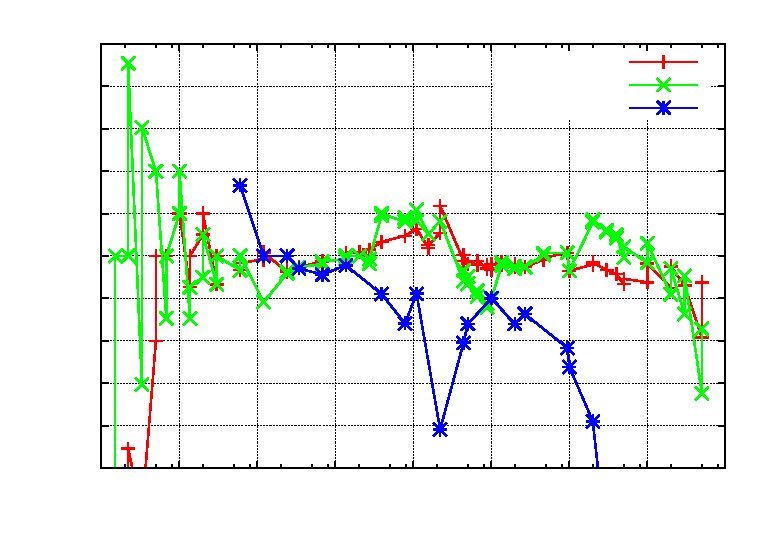
\includegraphics{../GNU/Mega8res}}%
    \gplfronttext
  \end{picture}%
\endgroup

\caption{Relativer Fehler für Widerstands-Messungen mit ATmega8 }
\label{fig:mega8res}
\end{figure}

\begin{figure}[H]
  \begin{subfigure}[b]{9cm}
    \centering
    \resizebox{9cm}{!}{% GNUPLOT: LaTeX picture with Postscript
\begingroup
  \makeatletter
  \providecommand\color[2][]{%
    \GenericError{(gnuplot) \space\space\space\@spaces}{%
      Package color not loaded in conjunction with
      terminal option `colourtext'%
    }{See the gnuplot documentation for explanation.%
    }{Either use 'blacktext' in gnuplot or load the package
      color.sty in LaTeX.}%
    \renewcommand\color[2][]{}%
  }%
  \providecommand\includegraphics[2][]{%
    \GenericError{(gnuplot) \space\space\space\@spaces}{%
      Package graphicx or graphics not loaded%
    }{See the gnuplot documentation for explanation.%
    }{The gnuplot epslatex terminal needs graphicx.sty or graphics.sty.}%
    \renewcommand\includegraphics[2][]{}%
  }%
  \providecommand\rotatebox[2]{#2}%
  \@ifundefined{ifGPcolor}{%
    \newif\ifGPcolor
    \GPcolortrue
  }{}%
  \@ifundefined{ifGPblacktext}{%
    \newif\ifGPblacktext
    \GPblacktexttrue
  }{}%
  % define a \g@addto@macro without @ in the name:
  \let\gplgaddtomacro\g@addto@macro
  % define empty templates for all commands taking text:
  \gdef\gplbacktext{}%
  \gdef\gplfronttext{}%
  \makeatother
  \ifGPblacktext
    % no textcolor at all
    \def\colorrgb#1{}%
    \def\colorgray#1{}%
  \else
    % gray or color?
    \ifGPcolor
      \def\colorrgb#1{\color[rgb]{#1}}%
      \def\colorgray#1{\color[gray]{#1}}%
      \expandafter\def\csname LTw\endcsname{\color{white}}%
      \expandafter\def\csname LTb\endcsname{\color{black}}%
      \expandafter\def\csname LTa\endcsname{\color{black}}%
      \expandafter\def\csname LT0\endcsname{\color[rgb]{1,0,0}}%
      \expandafter\def\csname LT1\endcsname{\color[rgb]{0,1,0}}%
      \expandafter\def\csname LT2\endcsname{\color[rgb]{0,0,1}}%
      \expandafter\def\csname LT3\endcsname{\color[rgb]{1,0,1}}%
      \expandafter\def\csname LT4\endcsname{\color[rgb]{0,1,1}}%
      \expandafter\def\csname LT5\endcsname{\color[rgb]{1,1,0}}%
      \expandafter\def\csname LT6\endcsname{\color[rgb]{0,0,0}}%
      \expandafter\def\csname LT7\endcsname{\color[rgb]{1,0.3,0}}%
      \expandafter\def\csname LT8\endcsname{\color[rgb]{0.5,0.5,0.5}}%
    \else
      % gray
      \def\colorrgb#1{\color{black}}%
      \def\colorgray#1{\color[gray]{#1}}%
      \expandafter\def\csname LTw\endcsname{\color{white}}%
      \expandafter\def\csname LTb\endcsname{\color{black}}%
      \expandafter\def\csname LTa\endcsname{\color{black}}%
      \expandafter\def\csname LT0\endcsname{\color{black}}%
      \expandafter\def\csname LT1\endcsname{\color{black}}%
      \expandafter\def\csname LT2\endcsname{\color{black}}%
      \expandafter\def\csname LT3\endcsname{\color{black}}%
      \expandafter\def\csname LT4\endcsname{\color{black}}%
      \expandafter\def\csname LT5\endcsname{\color{black}}%
      \expandafter\def\csname LT6\endcsname{\color{black}}%
      \expandafter\def\csname LT7\endcsname{\color{black}}%
      \expandafter\def\csname LT8\endcsname{\color{black}}%
    \fi
  \fi
  \setlength{\unitlength}{0.0500bp}%
  \begin{picture}(7200.00,5040.00)%
    \gplgaddtomacro\gplbacktext{%
      \csname LTb\endcsname%
      \put(682,704){\makebox(0,0)[r]{\strut{}-5}}%
      \csname LTb\endcsname%
      \put(682,1111){\makebox(0,0)[r]{\strut{}-4}}%
      \csname LTb\endcsname%
      \put(682,1518){\makebox(0,0)[r]{\strut{}-3}}%
      \csname LTb\endcsname%
      \put(682,1925){\makebox(0,0)[r]{\strut{}-2}}%
      \csname LTb\endcsname%
      \put(682,2332){\makebox(0,0)[r]{\strut{}-1}}%
      \csname LTb\endcsname%
      \put(682,2740){\makebox(0,0)[r]{\strut{} 0}}%
      \csname LTb\endcsname%
      \put(682,3147){\makebox(0,0)[r]{\strut{} 1}}%
      \csname LTb\endcsname%
      \put(682,3554){\makebox(0,0)[r]{\strut{} 2}}%
      \csname LTb\endcsname%
      \put(682,3961){\makebox(0,0)[r]{\strut{} 3}}%
      \csname LTb\endcsname%
      \put(682,4368){\makebox(0,0)[r]{\strut{} 4}}%
      \csname LTb\endcsname%
      \put(682,4775){\makebox(0,0)[r]{\strut{} 5}}%
      \csname LTb\endcsname%
      \put(814,484){\makebox(0,0){\strut{}1 }}%
      \csname LTb\endcsname%
      \put(1563,484){\makebox(0,0){\strut{}10 }}%
      \csname LTb\endcsname%
      \put(2311,484){\makebox(0,0){\strut{}100 }}%
      \csname LTb\endcsname%
      \put(3060,484){\makebox(0,0){\strut{}1k}}%
      \csname LTb\endcsname%
      \put(3809,484){\makebox(0,0){\strut{}10k}}%
      \csname LTb\endcsname%
      \put(4557,484){\makebox(0,0){\strut{}100k}}%
      \csname LTb\endcsname%
      \put(5306,484){\makebox(0,0){\strut{}1M}}%
      \csname LTb\endcsname%
      \put(6054,484){\makebox(0,0){\strut{}10M}}%
      \csname LTb\endcsname%
      \put(6803,484){\makebox(0,0){\strut{}100M}}%
      \put(176,2739){\rotatebox{-270}{\makebox(0,0){\strut{}Error / Percent}}}%
      \put(3808,154){\makebox(0,0){\strut{}Resistor value / Ohm}}%
    }%
    \gplgaddtomacro\gplfronttext{%
      \csname LTb\endcsname%
      \put(5753,4602){\makebox(0,0)[r]{\strut{}Mega8A-4}}%
      \csname LTb\endcsname%
      \put(5753,4382){\makebox(0,0)[r]{\strut{}Mega8A-5}}%
      \csname LTb\endcsname%
      \put(5753,4162){\makebox(0,0)[r]{\strut{}Mega8A-6}}%
    }%
    \gplbacktext
    \put(0,0){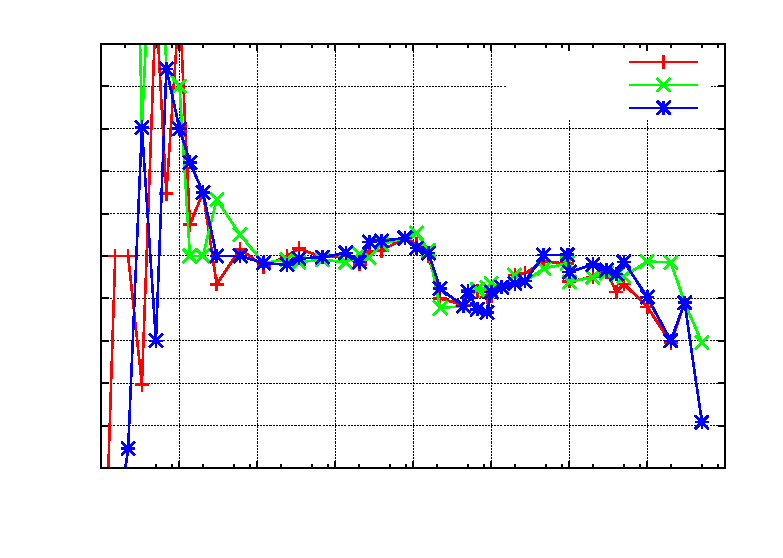
\includegraphics{../GNU/Mega8Ares}}%
    \gplfronttext
  \end{picture}%
\endgroup
}
    \caption{mit drei ATmega8A}
    \label{fig:mega8Ares}
  \end{subfigure}
  ~
  \begin{subfigure}[b]{9cm}
    \centering
    \resizebox{9cm}{!}{% GNUPLOT: LaTeX picture with Postscript
\begingroup
  \makeatletter
  \providecommand\color[2][]{%
    \GenericError{(gnuplot) \space\space\space\@spaces}{%
      Package color not loaded in conjunction with
      terminal option `colourtext'%
    }{See the gnuplot documentation for explanation.%
    }{Either use 'blacktext' in gnuplot or load the package
      color.sty in LaTeX.}%
    \renewcommand\color[2][]{}%
  }%
  \providecommand\includegraphics[2][]{%
    \GenericError{(gnuplot) \space\space\space\@spaces}{%
      Package graphicx or graphics not loaded%
    }{See the gnuplot documentation for explanation.%
    }{The gnuplot epslatex terminal needs graphicx.sty or graphics.sty.}%
    \renewcommand\includegraphics[2][]{}%
  }%
  \providecommand\rotatebox[2]{#2}%
  \@ifundefined{ifGPcolor}{%
    \newif\ifGPcolor
    \GPcolortrue
  }{}%
  \@ifundefined{ifGPblacktext}{%
    \newif\ifGPblacktext
    \GPblacktexttrue
  }{}%
  % define a \g@addto@macro without @ in the name:
  \let\gplgaddtomacro\g@addto@macro
  % define empty templates for all commands taking text:
  \gdef\gplbacktext{}%
  \gdef\gplfronttext{}%
  \makeatother
  \ifGPblacktext
    % no textcolor at all
    \def\colorrgb#1{}%
    \def\colorgray#1{}%
  \else
    % gray or color?
    \ifGPcolor
      \def\colorrgb#1{\color[rgb]{#1}}%
      \def\colorgray#1{\color[gray]{#1}}%
      \expandafter\def\csname LTw\endcsname{\color{white}}%
      \expandafter\def\csname LTb\endcsname{\color{black}}%
      \expandafter\def\csname LTa\endcsname{\color{black}}%
      \expandafter\def\csname LT0\endcsname{\color[rgb]{1,0,0}}%
      \expandafter\def\csname LT1\endcsname{\color[rgb]{0,1,0}}%
      \expandafter\def\csname LT2\endcsname{\color[rgb]{0,0,1}}%
      \expandafter\def\csname LT3\endcsname{\color[rgb]{1,0,1}}%
      \expandafter\def\csname LT4\endcsname{\color[rgb]{0,1,1}}%
      \expandafter\def\csname LT5\endcsname{\color[rgb]{1,1,0}}%
      \expandafter\def\csname LT6\endcsname{\color[rgb]{0,0,0}}%
      \expandafter\def\csname LT7\endcsname{\color[rgb]{1,0.3,0}}%
      \expandafter\def\csname LT8\endcsname{\color[rgb]{0.5,0.5,0.5}}%
    \else
      % gray
      \def\colorrgb#1{\color{black}}%
      \def\colorgray#1{\color[gray]{#1}}%
      \expandafter\def\csname LTw\endcsname{\color{white}}%
      \expandafter\def\csname LTb\endcsname{\color{black}}%
      \expandafter\def\csname LTa\endcsname{\color{black}}%
      \expandafter\def\csname LT0\endcsname{\color{black}}%
      \expandafter\def\csname LT1\endcsname{\color{black}}%
      \expandafter\def\csname LT2\endcsname{\color{black}}%
      \expandafter\def\csname LT3\endcsname{\color{black}}%
      \expandafter\def\csname LT4\endcsname{\color{black}}%
      \expandafter\def\csname LT5\endcsname{\color{black}}%
      \expandafter\def\csname LT6\endcsname{\color{black}}%
      \expandafter\def\csname LT7\endcsname{\color{black}}%
      \expandafter\def\csname LT8\endcsname{\color{black}}%
    \fi
  \fi
  \setlength{\unitlength}{0.0500bp}%
  \begin{picture}(7200.00,5040.00)%
    \gplgaddtomacro\gplbacktext{%
      \csname LTb\endcsname%
      \put(682,704){\makebox(0,0)[r]{\strut{}-5}}%
      \csname LTb\endcsname%
      \put(682,1111){\makebox(0,0)[r]{\strut{}-4}}%
      \csname LTb\endcsname%
      \put(682,1518){\makebox(0,0)[r]{\strut{}-3}}%
      \csname LTb\endcsname%
      \put(682,1925){\makebox(0,0)[r]{\strut{}-2}}%
      \csname LTb\endcsname%
      \put(682,2332){\makebox(0,0)[r]{\strut{}-1}}%
      \csname LTb\endcsname%
      \put(682,2740){\makebox(0,0)[r]{\strut{} 0}}%
      \csname LTb\endcsname%
      \put(682,3147){\makebox(0,0)[r]{\strut{} 1}}%
      \csname LTb\endcsname%
      \put(682,3554){\makebox(0,0)[r]{\strut{} 2}}%
      \csname LTb\endcsname%
      \put(682,3961){\makebox(0,0)[r]{\strut{} 3}}%
      \csname LTb\endcsname%
      \put(682,4368){\makebox(0,0)[r]{\strut{} 4}}%
      \csname LTb\endcsname%
      \put(682,4775){\makebox(0,0)[r]{\strut{} 5}}%
      \csname LTb\endcsname%
      \put(814,484){\makebox(0,0){\strut{}1 }}%
      \csname LTb\endcsname%
      \put(1563,484){\makebox(0,0){\strut{}10 }}%
      \csname LTb\endcsname%
      \put(2311,484){\makebox(0,0){\strut{}100 }}%
      \csname LTb\endcsname%
      \put(3060,484){\makebox(0,0){\strut{}1k}}%
      \csname LTb\endcsname%
      \put(3809,484){\makebox(0,0){\strut{}10k}}%
      \csname LTb\endcsname%
      \put(4557,484){\makebox(0,0){\strut{}100k}}%
      \csname LTb\endcsname%
      \put(5306,484){\makebox(0,0){\strut{}1M}}%
      \csname LTb\endcsname%
      \put(6054,484){\makebox(0,0){\strut{}10M}}%
      \csname LTb\endcsname%
      \put(6803,484){\makebox(0,0){\strut{}100M}}%
      \put(176,2739){\rotatebox{-270}{\makebox(0,0){\strut{}Error / Percent}}}%
      \put(3808,154){\makebox(0,0){\strut{}Resistor value / Ohm}}%
    }%
    \gplgaddtomacro\gplfronttext{%
      \csname LTb\endcsname%
      \put(5753,4602){\makebox(0,0)[r]{\strut{}Mega8L-7}}%
      \csname LTb\endcsname%
      \put(5753,4382){\makebox(0,0)[r]{\strut{}Mega8L-8}}%
      \csname LTb\endcsname%
      \put(5753,4162){\makebox(0,0)[r]{\strut{}Mega8L-9}}%
    }%
    \gplbacktext
    \put(0,0){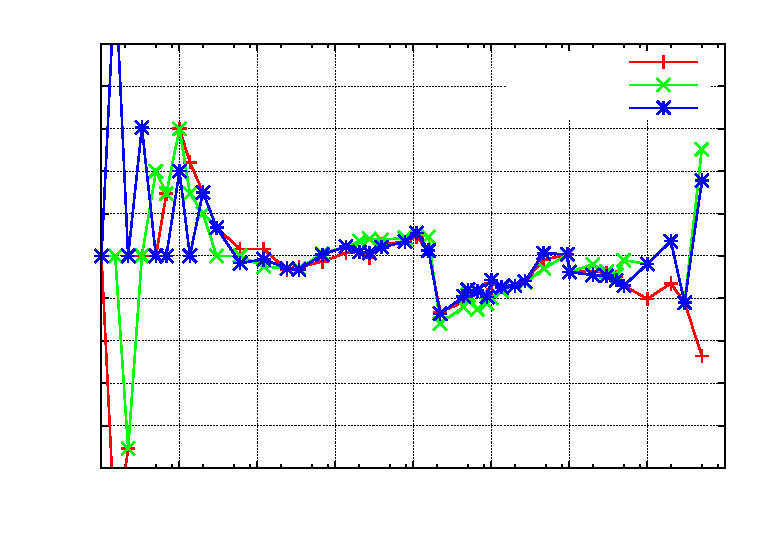
\includegraphics{../GNU/Mega8Lres}}%
    \gplfronttext
  \end{picture}%
\endgroup
}
    \caption{mit drei ATmega8L}
    \label{fig:mega8Lres}
  \end{subfigure}
\caption{Relativer Fehler für Widerstands-Messungen}
\end{figure}

\begin{figure}[H]
\centering
% GNUPLOT: LaTeX picture with Postscript
\begingroup
  \makeatletter
  \providecommand\color[2][]{%
    \GenericError{(gnuplot) \space\space\space\@spaces}{%
      Package color not loaded in conjunction with
      terminal option `colourtext'%
    }{See the gnuplot documentation for explanation.%
    }{Either use 'blacktext' in gnuplot or load the package
      color.sty in LaTeX.}%
    \renewcommand\color[2][]{}%
  }%
  \providecommand\includegraphics[2][]{%
    \GenericError{(gnuplot) \space\space\space\@spaces}{%
      Package graphicx or graphics not loaded%
    }{See the gnuplot documentation for explanation.%
    }{The gnuplot epslatex terminal needs graphicx.sty or graphics.sty.}%
    \renewcommand\includegraphics[2][]{}%
  }%
  \providecommand\rotatebox[2]{#2}%
  \@ifundefined{ifGPcolor}{%
    \newif\ifGPcolor
    \GPcolortrue
  }{}%
  \@ifundefined{ifGPblacktext}{%
    \newif\ifGPblacktext
    \GPblacktexttrue
  }{}%
  % define a \g@addto@macro without @ in the name:
  \let\gplgaddtomacro\g@addto@macro
  % define empty templates for all commands taking text:
  \gdef\gplbacktext{}%
  \gdef\gplfronttext{}%
  \makeatother
  \ifGPblacktext
    % no textcolor at all
    \def\colorrgb#1{}%
    \def\colorgray#1{}%
  \else
    % gray or color?
    \ifGPcolor
      \def\colorrgb#1{\color[rgb]{#1}}%
      \def\colorgray#1{\color[gray]{#1}}%
      \expandafter\def\csname LTw\endcsname{\color{white}}%
      \expandafter\def\csname LTb\endcsname{\color{black}}%
      \expandafter\def\csname LTa\endcsname{\color{black}}%
      \expandafter\def\csname LT0\endcsname{\color[rgb]{1,0,0}}%
      \expandafter\def\csname LT1\endcsname{\color[rgb]{0,1,0}}%
      \expandafter\def\csname LT2\endcsname{\color[rgb]{0,0,1}}%
      \expandafter\def\csname LT3\endcsname{\color[rgb]{1,0,1}}%
      \expandafter\def\csname LT4\endcsname{\color[rgb]{0,1,1}}%
      \expandafter\def\csname LT5\endcsname{\color[rgb]{1,1,0}}%
      \expandafter\def\csname LT6\endcsname{\color[rgb]{0,0,0}}%
      \expandafter\def\csname LT7\endcsname{\color[rgb]{1,0.3,0}}%
      \expandafter\def\csname LT8\endcsname{\color[rgb]{0.5,0.5,0.5}}%
    \else
      % gray
      \def\colorrgb#1{\color{black}}%
      \def\colorgray#1{\color[gray]{#1}}%
      \expandafter\def\csname LTw\endcsname{\color{white}}%
      \expandafter\def\csname LTb\endcsname{\color{black}}%
      \expandafter\def\csname LTa\endcsname{\color{black}}%
      \expandafter\def\csname LT0\endcsname{\color{black}}%
      \expandafter\def\csname LT1\endcsname{\color{black}}%
      \expandafter\def\csname LT2\endcsname{\color{black}}%
      \expandafter\def\csname LT3\endcsname{\color{black}}%
      \expandafter\def\csname LT4\endcsname{\color{black}}%
      \expandafter\def\csname LT5\endcsname{\color{black}}%
      \expandafter\def\csname LT6\endcsname{\color{black}}%
      \expandafter\def\csname LT7\endcsname{\color{black}}%
      \expandafter\def\csname LT8\endcsname{\color{black}}%
    \fi
  \fi
  \setlength{\unitlength}{0.0500bp}%
  \begin{picture}(7200.00,5040.00)%
    \gplgaddtomacro\gplbacktext{%
      \csname LTb\endcsname%
      \put(682,704){\makebox(0,0)[r]{\strut{}-5}}%
      \csname LTb\endcsname%
      \put(682,1111){\makebox(0,0)[r]{\strut{}-4}}%
      \csname LTb\endcsname%
      \put(682,1518){\makebox(0,0)[r]{\strut{}-3}}%
      \csname LTb\endcsname%
      \put(682,1925){\makebox(0,0)[r]{\strut{}-2}}%
      \csname LTb\endcsname%
      \put(682,2332){\makebox(0,0)[r]{\strut{}-1}}%
      \csname LTb\endcsname%
      \put(682,2740){\makebox(0,0)[r]{\strut{} 0}}%
      \csname LTb\endcsname%
      \put(682,3147){\makebox(0,0)[r]{\strut{} 1}}%
      \csname LTb\endcsname%
      \put(682,3554){\makebox(0,0)[r]{\strut{} 2}}%
      \csname LTb\endcsname%
      \put(682,3961){\makebox(0,0)[r]{\strut{} 3}}%
      \csname LTb\endcsname%
      \put(682,4368){\makebox(0,0)[r]{\strut{} 4}}%
      \csname LTb\endcsname%
      \put(682,4775){\makebox(0,0)[r]{\strut{} 5}}%
      \csname LTb\endcsname%
      \put(814,484){\makebox(0,0){\strut{}1 }}%
      \csname LTb\endcsname%
      \put(1563,484){\makebox(0,0){\strut{}10 }}%
      \csname LTb\endcsname%
      \put(2311,484){\makebox(0,0){\strut{}100 }}%
      \csname LTb\endcsname%
      \put(3060,484){\makebox(0,0){\strut{}1k}}%
      \csname LTb\endcsname%
      \put(3809,484){\makebox(0,0){\strut{}10k}}%
      \csname LTb\endcsname%
      \put(4557,484){\makebox(0,0){\strut{}100k}}%
      \csname LTb\endcsname%
      \put(5306,484){\makebox(0,0){\strut{}1M}}%
      \csname LTb\endcsname%
      \put(6054,484){\makebox(0,0){\strut{}10M}}%
      \csname LTb\endcsname%
      \put(6803,484){\makebox(0,0){\strut{}100M}}%
      \put(176,2739){\rotatebox{-270}{\makebox(0,0){\strut{}Error / Percent}}}%
      \put(3808,154){\makebox(0,0){\strut{}Resistor value / Ohm}}%
    }%
    \gplgaddtomacro\gplfronttext{%
      \csname LTb\endcsname%
      \put(5753,4602){\makebox(0,0)[r]{\strut{}Mega168}}%
      \csname LTb\endcsname%
      \put(5753,4382){\makebox(0,0)[r]{\strut{}Mega168as}}%
    }%
    \gplbacktext
    \put(0,0){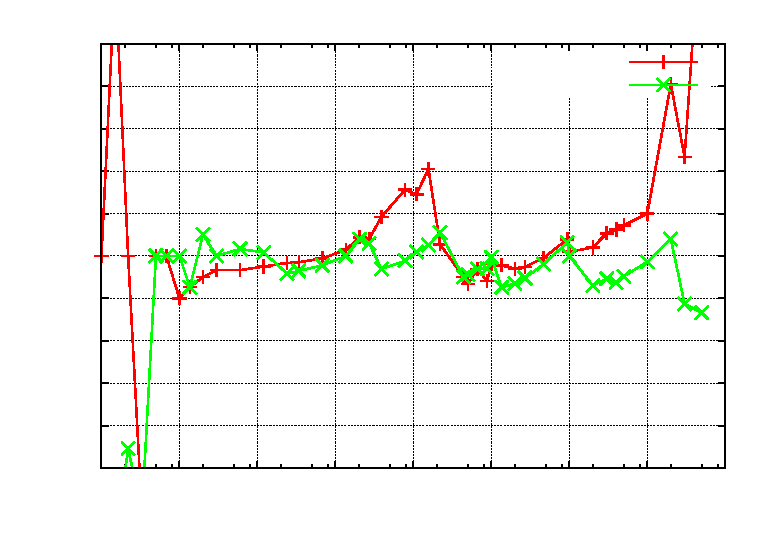
\includegraphics{../GNU/Mega168res}}%
    \gplfronttext
  \end{picture}%
\endgroup

\caption{Relativer Fehler für Widerstand-Messungen mit ATmega168 }
\label{fig:mega168res}
\end{figure}

Das Diagramm \ref{fig:m168res_all} zeigt die Messfehler von drei ATmega168-Prozessoren vor der Kalibration als Punkte, nach der
Kalibration als Linie. Entsprechend werden die Messfehler von drei ATmega168A in Abbildung \ref{fig:m168ares_all} und
die Messfehler von drei ATmega328P in Abbildung \ref{fig:m168pres_all} gezeigt.
Die Messfehler der ATmega328 werden in den Abbildungen \ref{fig:m328res_all} und \ref{fig:m328pres_all} gezeigt.
Nach der automatischen Kalibration bleibt der Messfehler mit einer Ausnahme (ATmega328P-13, \(22k\Omega\)) im Widerstandsbereich
\(10\Omega~-~20M\Omega\) im Bereich \(\pm1\%\).
Vor der Kalibration können die Messfehler bei einigen Prozessoren bis \(\pm~3\%\) betragen.
Der Fehler wird verursacht durch die AUTOSCALE\_ADC-Umschaltung der ADC-Referenz.
Durch den direkten Vergleich einer Kondensatorspannung von unter \(1V\), einmal mit der VCC-Referenz und nochmal mit
der internen ADC-Referenz gemessen, kann der Fehler ausgeglichen werden.
In diesem Fall wird die Spannung mit dem gleichen Multiplexer-Kanal gemessen und die Bandgap-Referenz ist auf den AREF-Pin
aufgeschaltet.
Die direkte Vermessung der Bandgap-Referenz durch die direkte Wahl des Multiplexer-Eingangs führt leider zu diesem Offset,
der entweder manuell mit der Option REF\_R\_KORR oder automatisch mit der Option AUTO\_CAL des Selbsttestes beseitigt werden kann.
Im AUTO\_CAL-Modus ist REF\_R\_KORR ein zusätzlicher Offset zur automatisch gefundenen Spannungsdifferenz.

\begin{figure}[H]
  \begin{subfigure}[b]{9cm}
    \centering
    \resizebox{9cm}{!}{% GNUPLOT: LaTeX picture with Postscript
\begingroup
  \makeatletter
  \providecommand\color[2][]{%
    \GenericError{(gnuplot) \space\space\space\@spaces}{%
      Package color not loaded in conjunction with
      terminal option `colourtext'%
    }{See the gnuplot documentation for explanation.%
    }{Either use 'blacktext' in gnuplot or load the package
      color.sty in LaTeX.}%
    \renewcommand\color[2][]{}%
  }%
  \providecommand\includegraphics[2][]{%
    \GenericError{(gnuplot) \space\space\space\@spaces}{%
      Package graphicx or graphics not loaded%
    }{See the gnuplot documentation for explanation.%
    }{The gnuplot epslatex terminal needs graphicx.sty or graphics.sty.}%
    \renewcommand\includegraphics[2][]{}%
  }%
  \providecommand\rotatebox[2]{#2}%
  \@ifundefined{ifGPcolor}{%
    \newif\ifGPcolor
    \GPcolortrue
  }{}%
  \@ifundefined{ifGPblacktext}{%
    \newif\ifGPblacktext
    \GPblacktexttrue
  }{}%
  % define a \g@addto@macro without @ in the name:
  \let\gplgaddtomacro\g@addto@macro
  % define empty templates for all commands taking text:
  \gdef\gplbacktext{}%
  \gdef\gplfronttext{}%
  \makeatother
  \ifGPblacktext
    % no textcolor at all
    \def\colorrgb#1{}%
    \def\colorgray#1{}%
  \else
    % gray or color?
    \ifGPcolor
      \def\colorrgb#1{\color[rgb]{#1}}%
      \def\colorgray#1{\color[gray]{#1}}%
      \expandafter\def\csname LTw\endcsname{\color{white}}%
      \expandafter\def\csname LTb\endcsname{\color{black}}%
      \expandafter\def\csname LTa\endcsname{\color{black}}%
      \expandafter\def\csname LT0\endcsname{\color[rgb]{1,0,0}}%
      \expandafter\def\csname LT1\endcsname{\color[rgb]{0,1,0}}%
      \expandafter\def\csname LT2\endcsname{\color[rgb]{0,0,1}}%
      \expandafter\def\csname LT3\endcsname{\color[rgb]{1,0,1}}%
      \expandafter\def\csname LT4\endcsname{\color[rgb]{0,1,1}}%
      \expandafter\def\csname LT5\endcsname{\color[rgb]{1,1,0}}%
      \expandafter\def\csname LT6\endcsname{\color[rgb]{0,0,0}}%
      \expandafter\def\csname LT7\endcsname{\color[rgb]{1,0.3,0}}%
      \expandafter\def\csname LT8\endcsname{\color[rgb]{0.5,0.5,0.5}}%
    \else
      % gray
      \def\colorrgb#1{\color{black}}%
      \def\colorgray#1{\color[gray]{#1}}%
      \expandafter\def\csname LTw\endcsname{\color{white}}%
      \expandafter\def\csname LTb\endcsname{\color{black}}%
      \expandafter\def\csname LTa\endcsname{\color{black}}%
      \expandafter\def\csname LT0\endcsname{\color{black}}%
      \expandafter\def\csname LT1\endcsname{\color{black}}%
      \expandafter\def\csname LT2\endcsname{\color{black}}%
      \expandafter\def\csname LT3\endcsname{\color{black}}%
      \expandafter\def\csname LT4\endcsname{\color{black}}%
      \expandafter\def\csname LT5\endcsname{\color{black}}%
      \expandafter\def\csname LT6\endcsname{\color{black}}%
      \expandafter\def\csname LT7\endcsname{\color{black}}%
      \expandafter\def\csname LT8\endcsname{\color{black}}%
    \fi
  \fi
  \setlength{\unitlength}{0.0500bp}%
  \begin{picture}(7200.00,5040.00)%
    \gplgaddtomacro\gplbacktext{%
      \csname LTb\endcsname%
      \put(682,704){\makebox(0,0)[r]{\strut{}-5}}%
      \csname LTb\endcsname%
      \put(682,1111){\makebox(0,0)[r]{\strut{}-4}}%
      \csname LTb\endcsname%
      \put(682,1518){\makebox(0,0)[r]{\strut{}-3}}%
      \csname LTb\endcsname%
      \put(682,1925){\makebox(0,0)[r]{\strut{}-2}}%
      \csname LTb\endcsname%
      \put(682,2332){\makebox(0,0)[r]{\strut{}-1}}%
      \csname LTb\endcsname%
      \put(682,2740){\makebox(0,0)[r]{\strut{} 0}}%
      \csname LTb\endcsname%
      \put(682,3147){\makebox(0,0)[r]{\strut{} 1}}%
      \csname LTb\endcsname%
      \put(682,3554){\makebox(0,0)[r]{\strut{} 2}}%
      \csname LTb\endcsname%
      \put(682,3961){\makebox(0,0)[r]{\strut{} 3}}%
      \csname LTb\endcsname%
      \put(682,4368){\makebox(0,0)[r]{\strut{} 4}}%
      \csname LTb\endcsname%
      \put(682,4775){\makebox(0,0)[r]{\strut{} 5}}%
      \csname LTb\endcsname%
      \put(814,484){\makebox(0,0){\strut{}1 }}%
      \csname LTb\endcsname%
      \put(1563,484){\makebox(0,0){\strut{}10 }}%
      \csname LTb\endcsname%
      \put(2311,484){\makebox(0,0){\strut{}100 }}%
      \csname LTb\endcsname%
      \put(3060,484){\makebox(0,0){\strut{}1k}}%
      \csname LTb\endcsname%
      \put(3809,484){\makebox(0,0){\strut{}10k}}%
      \csname LTb\endcsname%
      \put(4557,484){\makebox(0,0){\strut{}100k}}%
      \csname LTb\endcsname%
      \put(5306,484){\makebox(0,0){\strut{}1M}}%
      \csname LTb\endcsname%
      \put(6054,484){\makebox(0,0){\strut{}10M}}%
      \csname LTb\endcsname%
      \put(6803,484){\makebox(0,0){\strut{}100M}}%
      \put(176,2739){\rotatebox{-270}{\makebox(0,0){\strut{}Error / Percent}}}%
      \put(3808,154){\makebox(0,0){\strut{}Resistor value / Ohm}}%
    }%
    \gplgaddtomacro\gplfronttext{%
      \csname LTb\endcsname%
      \put(5753,4602){\makebox(0,0)[r]{\strut{}m168-1}}%
      \csname LTb\endcsname%
      \put(5753,4382){\makebox(0,0)[r]{\strut{}m168-2}}%
      \csname LTb\endcsname%
      \put(5753,4162){\makebox(0,0)[r]{\strut{}m168-3}}%
      \csname LTb\endcsname%
      \put(5753,3942){\makebox(0,0)[r]{\strut{}m168-1}}%
      \csname LTb\endcsname%
      \put(5753,3722){\makebox(0,0)[r]{\strut{}m168-2}}%
      \csname LTb\endcsname%
      \put(5753,3502){\makebox(0,0)[r]{\strut{}m168-3}}%
    }%
    \gplbacktext
    \put(0,0){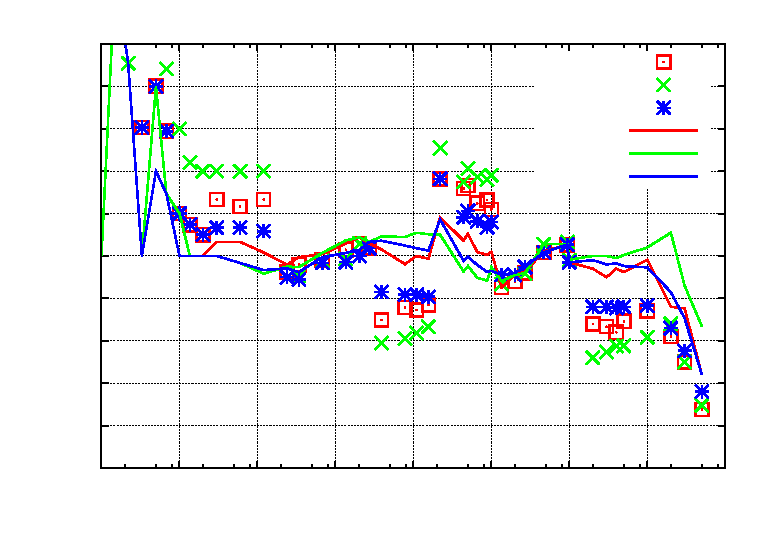
\includegraphics{../GNU/m168res_all}}%
    \gplfronttext
  \end{picture}%
\endgroup
}
    \caption{mit drei ATmega168}
    \label{fig:m168res_all}
  \end{subfigure}
  ~
  \begin{subfigure}[b]{9cm}
    \centering
    \resizebox{9cm}{!}{% GNUPLOT: LaTeX picture with Postscript
\begingroup
  \makeatletter
  \providecommand\color[2][]{%
    \GenericError{(gnuplot) \space\space\space\@spaces}{%
      Package color not loaded in conjunction with
      terminal option `colourtext'%
    }{See the gnuplot documentation for explanation.%
    }{Either use 'blacktext' in gnuplot or load the package
      color.sty in LaTeX.}%
    \renewcommand\color[2][]{}%
  }%
  \providecommand\includegraphics[2][]{%
    \GenericError{(gnuplot) \space\space\space\@spaces}{%
      Package graphicx or graphics not loaded%
    }{See the gnuplot documentation for explanation.%
    }{The gnuplot epslatex terminal needs graphicx.sty or graphics.sty.}%
    \renewcommand\includegraphics[2][]{}%
  }%
  \providecommand\rotatebox[2]{#2}%
  \@ifundefined{ifGPcolor}{%
    \newif\ifGPcolor
    \GPcolortrue
  }{}%
  \@ifundefined{ifGPblacktext}{%
    \newif\ifGPblacktext
    \GPblacktexttrue
  }{}%
  % define a \g@addto@macro without @ in the name:
  \let\gplgaddtomacro\g@addto@macro
  % define empty templates for all commands taking text:
  \gdef\gplbacktext{}%
  \gdef\gplfronttext{}%
  \makeatother
  \ifGPblacktext
    % no textcolor at all
    \def\colorrgb#1{}%
    \def\colorgray#1{}%
  \else
    % gray or color?
    \ifGPcolor
      \def\colorrgb#1{\color[rgb]{#1}}%
      \def\colorgray#1{\color[gray]{#1}}%
      \expandafter\def\csname LTw\endcsname{\color{white}}%
      \expandafter\def\csname LTb\endcsname{\color{black}}%
      \expandafter\def\csname LTa\endcsname{\color{black}}%
      \expandafter\def\csname LT0\endcsname{\color[rgb]{1,0,0}}%
      \expandafter\def\csname LT1\endcsname{\color[rgb]{0,1,0}}%
      \expandafter\def\csname LT2\endcsname{\color[rgb]{0,0,1}}%
      \expandafter\def\csname LT3\endcsname{\color[rgb]{1,0,1}}%
      \expandafter\def\csname LT4\endcsname{\color[rgb]{0,1,1}}%
      \expandafter\def\csname LT5\endcsname{\color[rgb]{1,1,0}}%
      \expandafter\def\csname LT6\endcsname{\color[rgb]{0,0,0}}%
      \expandafter\def\csname LT7\endcsname{\color[rgb]{1,0.3,0}}%
      \expandafter\def\csname LT8\endcsname{\color[rgb]{0.5,0.5,0.5}}%
    \else
      % gray
      \def\colorrgb#1{\color{black}}%
      \def\colorgray#1{\color[gray]{#1}}%
      \expandafter\def\csname LTw\endcsname{\color{white}}%
      \expandafter\def\csname LTb\endcsname{\color{black}}%
      \expandafter\def\csname LTa\endcsname{\color{black}}%
      \expandafter\def\csname LT0\endcsname{\color{black}}%
      \expandafter\def\csname LT1\endcsname{\color{black}}%
      \expandafter\def\csname LT2\endcsname{\color{black}}%
      \expandafter\def\csname LT3\endcsname{\color{black}}%
      \expandafter\def\csname LT4\endcsname{\color{black}}%
      \expandafter\def\csname LT5\endcsname{\color{black}}%
      \expandafter\def\csname LT6\endcsname{\color{black}}%
      \expandafter\def\csname LT7\endcsname{\color{black}}%
      \expandafter\def\csname LT8\endcsname{\color{black}}%
    \fi
  \fi
  \setlength{\unitlength}{0.0500bp}%
  \begin{picture}(7200.00,5040.00)%
    \gplgaddtomacro\gplbacktext{%
      \csname LTb\endcsname%
      \put(682,704){\makebox(0,0)[r]{\strut{}-5}}%
      \csname LTb\endcsname%
      \put(682,1111){\makebox(0,0)[r]{\strut{}-4}}%
      \csname LTb\endcsname%
      \put(682,1518){\makebox(0,0)[r]{\strut{}-3}}%
      \csname LTb\endcsname%
      \put(682,1925){\makebox(0,0)[r]{\strut{}-2}}%
      \csname LTb\endcsname%
      \put(682,2332){\makebox(0,0)[r]{\strut{}-1}}%
      \csname LTb\endcsname%
      \put(682,2740){\makebox(0,0)[r]{\strut{} 0}}%
      \csname LTb\endcsname%
      \put(682,3147){\makebox(0,0)[r]{\strut{} 1}}%
      \csname LTb\endcsname%
      \put(682,3554){\makebox(0,0)[r]{\strut{} 2}}%
      \csname LTb\endcsname%
      \put(682,3961){\makebox(0,0)[r]{\strut{} 3}}%
      \csname LTb\endcsname%
      \put(682,4368){\makebox(0,0)[r]{\strut{} 4}}%
      \csname LTb\endcsname%
      \put(682,4775){\makebox(0,0)[r]{\strut{} 5}}%
      \csname LTb\endcsname%
      \put(814,484){\makebox(0,0){\strut{}1 }}%
      \csname LTb\endcsname%
      \put(1563,484){\makebox(0,0){\strut{}10 }}%
      \csname LTb\endcsname%
      \put(2311,484){\makebox(0,0){\strut{}100 }}%
      \csname LTb\endcsname%
      \put(3060,484){\makebox(0,0){\strut{}1k}}%
      \csname LTb\endcsname%
      \put(3809,484){\makebox(0,0){\strut{}10k}}%
      \csname LTb\endcsname%
      \put(4557,484){\makebox(0,0){\strut{}100k}}%
      \csname LTb\endcsname%
      \put(5306,484){\makebox(0,0){\strut{}1M}}%
      \csname LTb\endcsname%
      \put(6054,484){\makebox(0,0){\strut{}10M}}%
      \csname LTb\endcsname%
      \put(6803,484){\makebox(0,0){\strut{}100M}}%
      \put(176,2739){\rotatebox{-270}{\makebox(0,0){\strut{}Error / Percent}}}%
      \put(3808,154){\makebox(0,0){\strut{}Resistor value / Ohm}}%
    }%
    \gplgaddtomacro\gplfronttext{%
      \csname LTb\endcsname%
      \put(5753,4602){\makebox(0,0)[r]{\strut{}m168a-4}}%
      \csname LTb\endcsname%
      \put(5753,4382){\makebox(0,0)[r]{\strut{}m168a-5}}%
      \csname LTb\endcsname%
      \put(5753,4162){\makebox(0,0)[r]{\strut{}m168a-6}}%
      \csname LTb\endcsname%
      \put(5753,3942){\makebox(0,0)[r]{\strut{}m168a-4}}%
      \csname LTb\endcsname%
      \put(5753,3722){\makebox(0,0)[r]{\strut{}m168a-5}}%
      \csname LTb\endcsname%
      \put(5753,3502){\makebox(0,0)[r]{\strut{}m168a-6}}%
    }%
    \gplbacktext
    \put(0,0){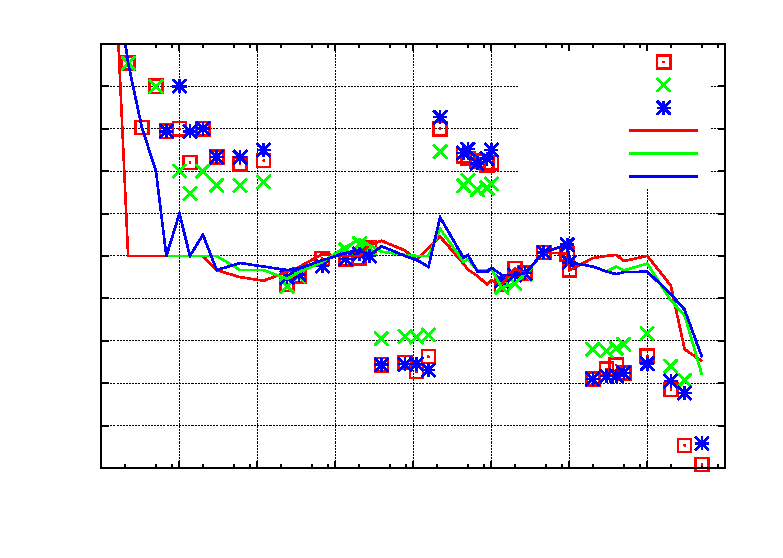
\includegraphics{../GNU/m168ares_all}}%
    \gplfronttext
  \end{picture}%
\endgroup
}
    \caption{mit drei ATmega168A}
    \label{fig:m168ares_all}
  \end{subfigure}
\caption{Relativer Fehler für Widerstands-Messungen}
\end{figure}

\begin{figure}[H]
\centering
% GNUPLOT: LaTeX picture with Postscript
\begingroup
  \makeatletter
  \providecommand\color[2][]{%
    \GenericError{(gnuplot) \space\space\space\@spaces}{%
      Package color not loaded in conjunction with
      terminal option `colourtext'%
    }{See the gnuplot documentation for explanation.%
    }{Either use 'blacktext' in gnuplot or load the package
      color.sty in LaTeX.}%
    \renewcommand\color[2][]{}%
  }%
  \providecommand\includegraphics[2][]{%
    \GenericError{(gnuplot) \space\space\space\@spaces}{%
      Package graphicx or graphics not loaded%
    }{See the gnuplot documentation for explanation.%
    }{The gnuplot epslatex terminal needs graphicx.sty or graphics.sty.}%
    \renewcommand\includegraphics[2][]{}%
  }%
  \providecommand\rotatebox[2]{#2}%
  \@ifundefined{ifGPcolor}{%
    \newif\ifGPcolor
    \GPcolortrue
  }{}%
  \@ifundefined{ifGPblacktext}{%
    \newif\ifGPblacktext
    \GPblacktexttrue
  }{}%
  % define a \g@addto@macro without @ in the name:
  \let\gplgaddtomacro\g@addto@macro
  % define empty templates for all commands taking text:
  \gdef\gplbacktext{}%
  \gdef\gplfronttext{}%
  \makeatother
  \ifGPblacktext
    % no textcolor at all
    \def\colorrgb#1{}%
    \def\colorgray#1{}%
  \else
    % gray or color?
    \ifGPcolor
      \def\colorrgb#1{\color[rgb]{#1}}%
      \def\colorgray#1{\color[gray]{#1}}%
      \expandafter\def\csname LTw\endcsname{\color{white}}%
      \expandafter\def\csname LTb\endcsname{\color{black}}%
      \expandafter\def\csname LTa\endcsname{\color{black}}%
      \expandafter\def\csname LT0\endcsname{\color[rgb]{1,0,0}}%
      \expandafter\def\csname LT1\endcsname{\color[rgb]{0,1,0}}%
      \expandafter\def\csname LT2\endcsname{\color[rgb]{0,0,1}}%
      \expandafter\def\csname LT3\endcsname{\color[rgb]{1,0,1}}%
      \expandafter\def\csname LT4\endcsname{\color[rgb]{0,1,1}}%
      \expandafter\def\csname LT5\endcsname{\color[rgb]{1,1,0}}%
      \expandafter\def\csname LT6\endcsname{\color[rgb]{0,0,0}}%
      \expandafter\def\csname LT7\endcsname{\color[rgb]{1,0.3,0}}%
      \expandafter\def\csname LT8\endcsname{\color[rgb]{0.5,0.5,0.5}}%
    \else
      % gray
      \def\colorrgb#1{\color{black}}%
      \def\colorgray#1{\color[gray]{#1}}%
      \expandafter\def\csname LTw\endcsname{\color{white}}%
      \expandafter\def\csname LTb\endcsname{\color{black}}%
      \expandafter\def\csname LTa\endcsname{\color{black}}%
      \expandafter\def\csname LT0\endcsname{\color{black}}%
      \expandafter\def\csname LT1\endcsname{\color{black}}%
      \expandafter\def\csname LT2\endcsname{\color{black}}%
      \expandafter\def\csname LT3\endcsname{\color{black}}%
      \expandafter\def\csname LT4\endcsname{\color{black}}%
      \expandafter\def\csname LT5\endcsname{\color{black}}%
      \expandafter\def\csname LT6\endcsname{\color{black}}%
      \expandafter\def\csname LT7\endcsname{\color{black}}%
      \expandafter\def\csname LT8\endcsname{\color{black}}%
    \fi
  \fi
  \setlength{\unitlength}{0.0500bp}%
  \begin{picture}(7200.00,5040.00)%
    \gplgaddtomacro\gplbacktext{%
      \csname LTb\endcsname%
      \put(682,704){\makebox(0,0)[r]{\strut{}-5}}%
      \csname LTb\endcsname%
      \put(682,1111){\makebox(0,0)[r]{\strut{}-4}}%
      \csname LTb\endcsname%
      \put(682,1518){\makebox(0,0)[r]{\strut{}-3}}%
      \csname LTb\endcsname%
      \put(682,1925){\makebox(0,0)[r]{\strut{}-2}}%
      \csname LTb\endcsname%
      \put(682,2332){\makebox(0,0)[r]{\strut{}-1}}%
      \csname LTb\endcsname%
      \put(682,2740){\makebox(0,0)[r]{\strut{} 0}}%
      \csname LTb\endcsname%
      \put(682,3147){\makebox(0,0)[r]{\strut{} 1}}%
      \csname LTb\endcsname%
      \put(682,3554){\makebox(0,0)[r]{\strut{} 2}}%
      \csname LTb\endcsname%
      \put(682,3961){\makebox(0,0)[r]{\strut{} 3}}%
      \csname LTb\endcsname%
      \put(682,4368){\makebox(0,0)[r]{\strut{} 4}}%
      \csname LTb\endcsname%
      \put(682,4775){\makebox(0,0)[r]{\strut{} 5}}%
      \csname LTb\endcsname%
      \put(814,484){\makebox(0,0){\strut{}1 }}%
      \csname LTb\endcsname%
      \put(1563,484){\makebox(0,0){\strut{}10 }}%
      \csname LTb\endcsname%
      \put(2311,484){\makebox(0,0){\strut{}100 }}%
      \csname LTb\endcsname%
      \put(3060,484){\makebox(0,0){\strut{}1k}}%
      \csname LTb\endcsname%
      \put(3809,484){\makebox(0,0){\strut{}10k}}%
      \csname LTb\endcsname%
      \put(4557,484){\makebox(0,0){\strut{}100k}}%
      \csname LTb\endcsname%
      \put(5306,484){\makebox(0,0){\strut{}1M}}%
      \csname LTb\endcsname%
      \put(6054,484){\makebox(0,0){\strut{}10M}}%
      \csname LTb\endcsname%
      \put(6803,484){\makebox(0,0){\strut{}100M}}%
      \put(176,2739){\rotatebox{-270}{\makebox(0,0){\strut{}Error / Percent}}}%
      \put(3808,154){\makebox(0,0){\strut{}Resistor value / Ohm}}%
    }%
    \gplgaddtomacro\gplfronttext{%
      \csname LTb\endcsname%
      \put(5753,4602){\makebox(0,0)[r]{\strut{}m168p-7}}%
      \csname LTb\endcsname%
      \put(5753,4382){\makebox(0,0)[r]{\strut{}m168p-8}}%
      \csname LTb\endcsname%
      \put(5753,4162){\makebox(0,0)[r]{\strut{}m168p-9}}%
      \csname LTb\endcsname%
      \put(5753,3942){\makebox(0,0)[r]{\strut{}m168p-7}}%
      \csname LTb\endcsname%
      \put(5753,3722){\makebox(0,0)[r]{\strut{}m168p-8}}%
      \csname LTb\endcsname%
      \put(5753,3502){\makebox(0,0)[r]{\strut{}m168p-9}}%
    }%
    \gplbacktext
    \put(0,0){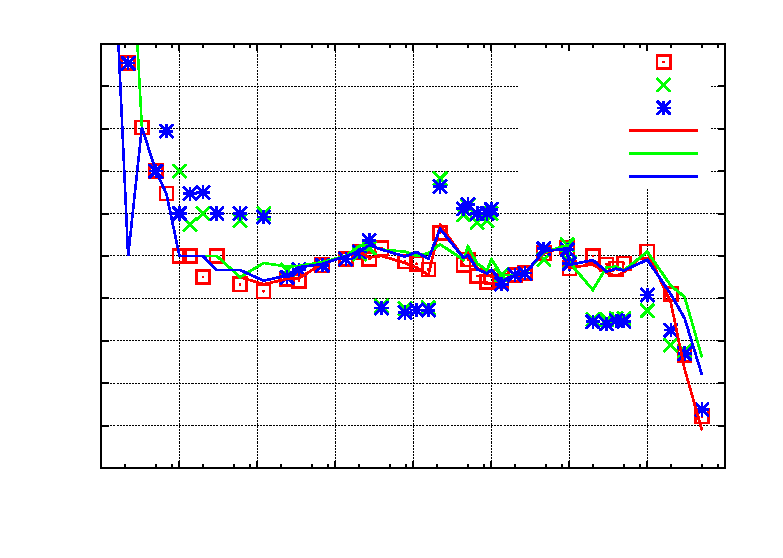
\includegraphics{../GNU/m168pres_all}}%
    \gplfronttext
  \end{picture}%
\endgroup

\caption{Relativer Fehler für Widerstands-Messungen mit drei ATmega168P }
\label{fig:m168pres_all}
\end{figure}

\begin{figure}[H]
  \begin{subfigure}[b]{9cm}
    \centering
    \resizebox{9cm}{!}{% GNUPLOT: LaTeX picture with Postscript
\begingroup
  \makeatletter
  \providecommand\color[2][]{%
    \GenericError{(gnuplot) \space\space\space\@spaces}{%
      Package color not loaded in conjunction with
      terminal option `colourtext'%
    }{See the gnuplot documentation for explanation.%
    }{Either use 'blacktext' in gnuplot or load the package
      color.sty in LaTeX.}%
    \renewcommand\color[2][]{}%
  }%
  \providecommand\includegraphics[2][]{%
    \GenericError{(gnuplot) \space\space\space\@spaces}{%
      Package graphicx or graphics not loaded%
    }{See the gnuplot documentation for explanation.%
    }{The gnuplot epslatex terminal needs graphicx.sty or graphics.sty.}%
    \renewcommand\includegraphics[2][]{}%
  }%
  \providecommand\rotatebox[2]{#2}%
  \@ifundefined{ifGPcolor}{%
    \newif\ifGPcolor
    \GPcolortrue
  }{}%
  \@ifundefined{ifGPblacktext}{%
    \newif\ifGPblacktext
    \GPblacktexttrue
  }{}%
  % define a \g@addto@macro without @ in the name:
  \let\gplgaddtomacro\g@addto@macro
  % define empty templates for all commands taking text:
  \gdef\gplbacktext{}%
  \gdef\gplfronttext{}%
  \makeatother
  \ifGPblacktext
    % no textcolor at all
    \def\colorrgb#1{}%
    \def\colorgray#1{}%
  \else
    % gray or color?
    \ifGPcolor
      \def\colorrgb#1{\color[rgb]{#1}}%
      \def\colorgray#1{\color[gray]{#1}}%
      \expandafter\def\csname LTw\endcsname{\color{white}}%
      \expandafter\def\csname LTb\endcsname{\color{black}}%
      \expandafter\def\csname LTa\endcsname{\color{black}}%
      \expandafter\def\csname LT0\endcsname{\color[rgb]{1,0,0}}%
      \expandafter\def\csname LT1\endcsname{\color[rgb]{0,1,0}}%
      \expandafter\def\csname LT2\endcsname{\color[rgb]{0,0,1}}%
      \expandafter\def\csname LT3\endcsname{\color[rgb]{1,0,1}}%
      \expandafter\def\csname LT4\endcsname{\color[rgb]{0,1,1}}%
      \expandafter\def\csname LT5\endcsname{\color[rgb]{1,1,0}}%
      \expandafter\def\csname LT6\endcsname{\color[rgb]{0,0,0}}%
      \expandafter\def\csname LT7\endcsname{\color[rgb]{1,0.3,0}}%
      \expandafter\def\csname LT8\endcsname{\color[rgb]{0.5,0.5,0.5}}%
    \else
      % gray
      \def\colorrgb#1{\color{black}}%
      \def\colorgray#1{\color[gray]{#1}}%
      \expandafter\def\csname LTw\endcsname{\color{white}}%
      \expandafter\def\csname LTb\endcsname{\color{black}}%
      \expandafter\def\csname LTa\endcsname{\color{black}}%
      \expandafter\def\csname LT0\endcsname{\color{black}}%
      \expandafter\def\csname LT1\endcsname{\color{black}}%
      \expandafter\def\csname LT2\endcsname{\color{black}}%
      \expandafter\def\csname LT3\endcsname{\color{black}}%
      \expandafter\def\csname LT4\endcsname{\color{black}}%
      \expandafter\def\csname LT5\endcsname{\color{black}}%
      \expandafter\def\csname LT6\endcsname{\color{black}}%
      \expandafter\def\csname LT7\endcsname{\color{black}}%
      \expandafter\def\csname LT8\endcsname{\color{black}}%
    \fi
  \fi
  \setlength{\unitlength}{0.0500bp}%
  \begin{picture}(7200.00,5040.00)%
    \gplgaddtomacro\gplbacktext{%
      \csname LTb\endcsname%
      \put(682,704){\makebox(0,0)[r]{\strut{}-5}}%
      \csname LTb\endcsname%
      \put(682,1111){\makebox(0,0)[r]{\strut{}-4}}%
      \csname LTb\endcsname%
      \put(682,1518){\makebox(0,0)[r]{\strut{}-3}}%
      \csname LTb\endcsname%
      \put(682,1925){\makebox(0,0)[r]{\strut{}-2}}%
      \csname LTb\endcsname%
      \put(682,2332){\makebox(0,0)[r]{\strut{}-1}}%
      \csname LTb\endcsname%
      \put(682,2740){\makebox(0,0)[r]{\strut{} 0}}%
      \csname LTb\endcsname%
      \put(682,3147){\makebox(0,0)[r]{\strut{} 1}}%
      \csname LTb\endcsname%
      \put(682,3554){\makebox(0,0)[r]{\strut{} 2}}%
      \csname LTb\endcsname%
      \put(682,3961){\makebox(0,0)[r]{\strut{} 3}}%
      \csname LTb\endcsname%
      \put(682,4368){\makebox(0,0)[r]{\strut{} 4}}%
      \csname LTb\endcsname%
      \put(682,4775){\makebox(0,0)[r]{\strut{} 5}}%
      \csname LTb\endcsname%
      \put(814,484){\makebox(0,0){\strut{}1 }}%
      \csname LTb\endcsname%
      \put(1563,484){\makebox(0,0){\strut{}10 }}%
      \csname LTb\endcsname%
      \put(2311,484){\makebox(0,0){\strut{}100 }}%
      \csname LTb\endcsname%
      \put(3060,484){\makebox(0,0){\strut{}1k}}%
      \csname LTb\endcsname%
      \put(3809,484){\makebox(0,0){\strut{}10k}}%
      \csname LTb\endcsname%
      \put(4557,484){\makebox(0,0){\strut{}100k}}%
      \csname LTb\endcsname%
      \put(5306,484){\makebox(0,0){\strut{}1M}}%
      \csname LTb\endcsname%
      \put(6054,484){\makebox(0,0){\strut{}10M}}%
      \csname LTb\endcsname%
      \put(6803,484){\makebox(0,0){\strut{}100M}}%
      \put(176,2739){\rotatebox{-270}{\makebox(0,0){\strut{}Error / Percent}}}%
      \put(3808,154){\makebox(0,0){\strut{}Resistor value / Ohm}}%
    }%
    \gplgaddtomacro\gplfronttext{%
      \csname LTb\endcsname%
      \put(5753,4602){\makebox(0,0)[r]{\strut{}m328-10}}%
      \csname LTb\endcsname%
      \put(5753,4382){\makebox(0,0)[r]{\strut{}m328-11}}%
      \csname LTb\endcsname%
      \put(5753,4162){\makebox(0,0)[r]{\strut{}m328-12}}%
      \csname LTb\endcsname%
      \put(5753,3942){\makebox(0,0)[r]{\strut{}m328-10}}%
      \csname LTb\endcsname%
      \put(5753,3722){\makebox(0,0)[r]{\strut{}m328-11}}%
      \csname LTb\endcsname%
      \put(5753,3502){\makebox(0,0)[r]{\strut{}m328-12}}%
    }%
    \gplbacktext
    \put(0,0){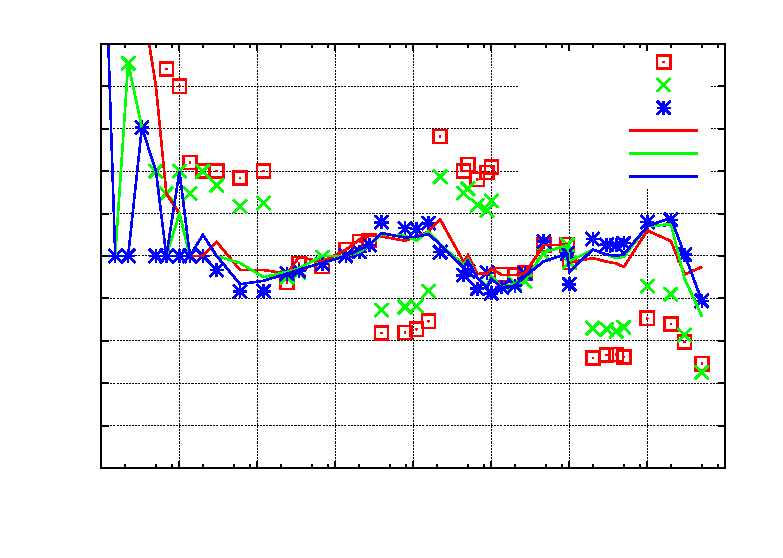
\includegraphics{../GNU/m328res_all}}%
    \gplfronttext
  \end{picture}%
\endgroup
}
    \caption{mit drei ATmega328}
    \label{fig:m328res_all}
  \end{subfigure}
  ~
  \begin{subfigure}[b]{9cm}
    \centering
    \resizebox{9cm}{!}{% GNUPLOT: LaTeX picture with Postscript
\begingroup
  \makeatletter
  \providecommand\color[2][]{%
    \GenericError{(gnuplot) \space\space\space\@spaces}{%
      Package color not loaded in conjunction with
      terminal option `colourtext'%
    }{See the gnuplot documentation for explanation.%
    }{Either use 'blacktext' in gnuplot or load the package
      color.sty in LaTeX.}%
    \renewcommand\color[2][]{}%
  }%
  \providecommand\includegraphics[2][]{%
    \GenericError{(gnuplot) \space\space\space\@spaces}{%
      Package graphicx or graphics not loaded%
    }{See the gnuplot documentation for explanation.%
    }{The gnuplot epslatex terminal needs graphicx.sty or graphics.sty.}%
    \renewcommand\includegraphics[2][]{}%
  }%
  \providecommand\rotatebox[2]{#2}%
  \@ifundefined{ifGPcolor}{%
    \newif\ifGPcolor
    \GPcolortrue
  }{}%
  \@ifundefined{ifGPblacktext}{%
    \newif\ifGPblacktext
    \GPblacktexttrue
  }{}%
  % define a \g@addto@macro without @ in the name:
  \let\gplgaddtomacro\g@addto@macro
  % define empty templates for all commands taking text:
  \gdef\gplbacktext{}%
  \gdef\gplfronttext{}%
  \makeatother
  \ifGPblacktext
    % no textcolor at all
    \def\colorrgb#1{}%
    \def\colorgray#1{}%
  \else
    % gray or color?
    \ifGPcolor
      \def\colorrgb#1{\color[rgb]{#1}}%
      \def\colorgray#1{\color[gray]{#1}}%
      \expandafter\def\csname LTw\endcsname{\color{white}}%
      \expandafter\def\csname LTb\endcsname{\color{black}}%
      \expandafter\def\csname LTa\endcsname{\color{black}}%
      \expandafter\def\csname LT0\endcsname{\color[rgb]{1,0,0}}%
      \expandafter\def\csname LT1\endcsname{\color[rgb]{0,1,0}}%
      \expandafter\def\csname LT2\endcsname{\color[rgb]{0,0,1}}%
      \expandafter\def\csname LT3\endcsname{\color[rgb]{1,0,1}}%
      \expandafter\def\csname LT4\endcsname{\color[rgb]{0,1,1}}%
      \expandafter\def\csname LT5\endcsname{\color[rgb]{1,1,0}}%
      \expandafter\def\csname LT6\endcsname{\color[rgb]{0,0,0}}%
      \expandafter\def\csname LT7\endcsname{\color[rgb]{1,0.3,0}}%
      \expandafter\def\csname LT8\endcsname{\color[rgb]{0.5,0.5,0.5}}%
    \else
      % gray
      \def\colorrgb#1{\color{black}}%
      \def\colorgray#1{\color[gray]{#1}}%
      \expandafter\def\csname LTw\endcsname{\color{white}}%
      \expandafter\def\csname LTb\endcsname{\color{black}}%
      \expandafter\def\csname LTa\endcsname{\color{black}}%
      \expandafter\def\csname LT0\endcsname{\color{black}}%
      \expandafter\def\csname LT1\endcsname{\color{black}}%
      \expandafter\def\csname LT2\endcsname{\color{black}}%
      \expandafter\def\csname LT3\endcsname{\color{black}}%
      \expandafter\def\csname LT4\endcsname{\color{black}}%
      \expandafter\def\csname LT5\endcsname{\color{black}}%
      \expandafter\def\csname LT6\endcsname{\color{black}}%
      \expandafter\def\csname LT7\endcsname{\color{black}}%
      \expandafter\def\csname LT8\endcsname{\color{black}}%
    \fi
  \fi
  \setlength{\unitlength}{0.0500bp}%
  \begin{picture}(7200.00,5040.00)%
    \gplgaddtomacro\gplbacktext{%
      \csname LTb\endcsname%
      \put(682,704){\makebox(0,0)[r]{\strut{}-5}}%
      \csname LTb\endcsname%
      \put(682,1111){\makebox(0,0)[r]{\strut{}-4}}%
      \csname LTb\endcsname%
      \put(682,1518){\makebox(0,0)[r]{\strut{}-3}}%
      \csname LTb\endcsname%
      \put(682,1925){\makebox(0,0)[r]{\strut{}-2}}%
      \csname LTb\endcsname%
      \put(682,2332){\makebox(0,0)[r]{\strut{}-1}}%
      \csname LTb\endcsname%
      \put(682,2740){\makebox(0,0)[r]{\strut{} 0}}%
      \csname LTb\endcsname%
      \put(682,3147){\makebox(0,0)[r]{\strut{} 1}}%
      \csname LTb\endcsname%
      \put(682,3554){\makebox(0,0)[r]{\strut{} 2}}%
      \csname LTb\endcsname%
      \put(682,3961){\makebox(0,0)[r]{\strut{} 3}}%
      \csname LTb\endcsname%
      \put(682,4368){\makebox(0,0)[r]{\strut{} 4}}%
      \csname LTb\endcsname%
      \put(682,4775){\makebox(0,0)[r]{\strut{} 5}}%
      \csname LTb\endcsname%
      \put(814,484){\makebox(0,0){\strut{}1 }}%
      \csname LTb\endcsname%
      \put(1563,484){\makebox(0,0){\strut{}10 }}%
      \csname LTb\endcsname%
      \put(2311,484){\makebox(0,0){\strut{}100 }}%
      \csname LTb\endcsname%
      \put(3060,484){\makebox(0,0){\strut{}1k}}%
      \csname LTb\endcsname%
      \put(3809,484){\makebox(0,0){\strut{}10k}}%
      \csname LTb\endcsname%
      \put(4557,484){\makebox(0,0){\strut{}100k}}%
      \csname LTb\endcsname%
      \put(5306,484){\makebox(0,0){\strut{}1M}}%
      \csname LTb\endcsname%
      \put(6054,484){\makebox(0,0){\strut{}10M}}%
      \csname LTb\endcsname%
      \put(6803,484){\makebox(0,0){\strut{}100M}}%
      \put(176,2739){\rotatebox{-270}{\makebox(0,0){\strut{}Error / Percent}}}%
      \put(3808,154){\makebox(0,0){\strut{}Resistor value / Ohm}}%
    }%
    \gplgaddtomacro\gplfronttext{%
      \csname LTb\endcsname%
      \put(5753,4602){\makebox(0,0)[r]{\strut{}m328p-13}}%
      \csname LTb\endcsname%
      \put(5753,4382){\makebox(0,0)[r]{\strut{}m328p-14}}%
      \csname LTb\endcsname%
      \put(5753,4162){\makebox(0,0)[r]{\strut{}m328p-15}}%
      \csname LTb\endcsname%
      \put(5753,3942){\makebox(0,0)[r]{\strut{}m328p-13}}%
      \csname LTb\endcsname%
      \put(5753,3722){\makebox(0,0)[r]{\strut{}m328p-14}}%
      \csname LTb\endcsname%
      \put(5753,3502){\makebox(0,0)[r]{\strut{}m328p-15}}%
    }%
    \gplbacktext
    \put(0,0){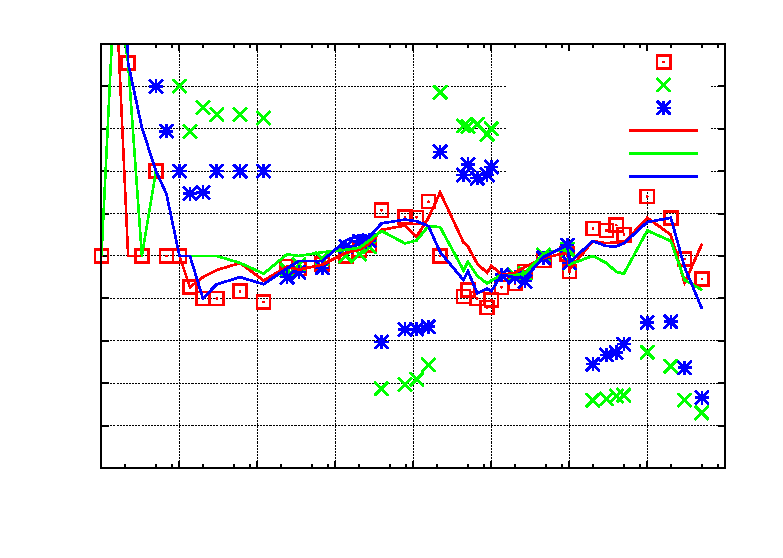
\includegraphics{../GNU/m328pres_all}}%
    \gplfronttext
  \end{picture}%
\endgroup
}
    \caption{mit drei ATmega328P}
    \label{fig:m328pres_all}
  \end{subfigure}
\caption{Relativer Fehler für Widerstands-Messungen}
\end{figure}


 \section{Messen von Kondensatoren}
Die Messung von Kapazitätswerten wird nach allen anderen Messungen als separater Teil mit einer Ladezeitmessung 
durchgeführt.
Die Originalsoftware vom Markus F. hat das mit einer Programmschleife gemacht, die den betreffenden digitalen
Eingangs-Pin bis zu einer Signaländerung gelesen hat und dabei die Schleifendurchläufe gezählt.
Dies hat den Nachteil, dass die Auflösung der Zeitmessung begrenzt ist durch die Gesamtzeit eines Schleifendurchlaufs.
Dies wurde üblicherweise in allen sechs Kombinationsmöglichkeiten für die drei Testpins durchgeführt.
Die aktuelle Software benutzt zwei verschiedene Möglichkeiten, um die Ladezeit in nur drei
Kombinationsmöglichkeiten für die drei Testpins zu erhalten.
Die positive Seite ist nun immer die höhere Testpin-Nummer.
Nur wenn die Kapazität zusammen mit einer parallel geschalteten Diode gemessen wird,
kann die Polarität die andere Richtung haben.

\subsection{Entladen der Kondensatoren}
Sie sollten die Kapazitäten immer entladen, bevor sie mit dem Tester verbunden werden.
Bevor irgendein Test gestartet wird, wird der Kondensator vom Tester immer noch einmal entladen.
Wenn die Spannung unter 1300mV ist, wird der Kondensator dafür mit den angeschlossenen ADC-Ports (Port C) kurzgeschlossen.
Ich glaube das ist in Ordnung, weil jeder Portausgang einen Innenwiderstand von ungefähr \(20\Omega\) hat.
Die Abbildung 149 (Seite 258) im Atmega8-Datenblatt \cite{ATmega8} zeigt einen Spannungsabfall an Ausgabe-Pins von bis zu 2V.
Natürlich kann ich nicht garantieren, dass kein Schaden auftreten kann.
Ich habe die Funktion mit Kondensatoren von mehr als \(15 mF\) sehr oft getestet und ich habe noch nie ein Problem bemerkt.
Der Strom sollte unter der spezifizierten Grenze von 40mA bleiben und reduziert sich schnell durch die Entladung.
Natürlich kann ein Schaden entstehen, wenn Sie einen (Hochvolt-) Kondensator nicht vollständig entladen, bevor Sie ihn an den Tester anschließen.

\subsection{Messung von großen Kapazitäten}
\label{sec:bigcap}
Eine Seite des Kondensators ist mit GND verbunden. Die andere Seite wird über den \(680\Omega\)-Widerstand für 10ms mit VCC verbunden.
Danach wird dieser Messpin auf Eingang geschaltet (hochohmig).
Nach diesem Strompuls wird die Spannung am Kondensator stromlos gemessen.
Wenn die Spannung noch nicht den Minimalwert von 300mV erreicht hat, wird dieser Ladepuls bis zu weiteren 499 Mal wiederholt.
Wenn nach 127 Pulsen (ungefähr 2s) noch nicht eine Minimalspannung von 75mV erreicht ist, wird der Ladevorgang abgebrochen,
 weil die 300mV mit den verbleibenden Ladepulsen nie erreicht werden wird.
Abbildung~\ref{fig:bigcap1} zeigt die drei Phasen der Kapazitätsbestimmung eines Kondensators.
Der Kapazitätswert wird dann berechnet aus der Ladepuls-Anzahl und der erreichten Ladespannung über eine Tabelle.
Die Tabelle enthält mit einem Spannungsabstand von 25mV die Faktoren, um aus der Ladezeit und der Spannung 
den Kapazitätswert zu bestimmen. 
Zwischenwerte der Spannung werden interpoliert.

\begin{figure}[H]
\centering

\includegraphics[]{../FIG/Bigcap.eps}
\caption{Kondensator-Entladung und -Ladung mit 10ms Ladepulsen bis zur Spannung \textgreater 300mV}
\label{fig:bigcap1}
\end{figure}

Wegen der niedrigen Ladespannung wird die Messung viel schneller als bei der ursprünglichen Softwareversion,
weil dieser Vorteil auch bei der Entladung wirkt. So können auch grössere Kondensatoren gemessen werden.
Zusätzlich stört in den meisten Fällen eine parallel geschaltete Diode nicht die Messung, weil die Schwellspannung
der Diode nicht erreicht wird.
Abbildung~\ref{pic:c229} zeigt das Laden und Entladen eines \(229\mu F\) großen Kondensators.
Das flache Dach der Messkurve bis zum Entladebeginn ist durch die Messzeit und Berechnungszeit des ATmega verursacht.
Abbildung~\ref{pic:c5mF} zeigt die gleiche Messung mit einem~\(5mF\)-Kondensator,
beachte wie die Messzeit inklusive Entladung auf ungefähr 1,5 Sekunden angewachsen ist.
Das letzte Beispiel in Abbildung~\ref{pic:c15mF} zeigt die Messung eines \(15mF\)-Kondensators.

\begin{figure}[H]
  \begin{subfigure}[b]{9cm}
    \centering
    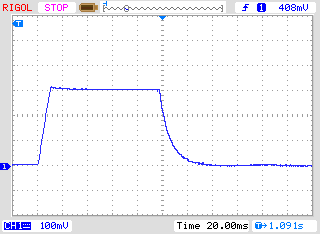
\includegraphics[width=9cm]{../PNG/charge_229uF.png}
    \caption{\(229\mu F\)-Kondensator}
    \label{pic:c229}
  \end{subfigure}
  ~
  \begin{subfigure}[b]{9cm}
    \centering
    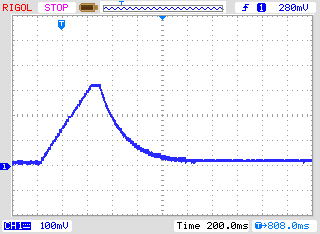
\includegraphics[width=9cm]{../PNG/charge_5mF.png}
    \caption{\(5mF\)-Kondensator}
    \label{pic:c5mF}
  \end{subfigure}
  \caption{Laden und Entladen von großen Kondensatoren für die Messung}
\end{figure}

\begin{figure}[H]
  \centering
    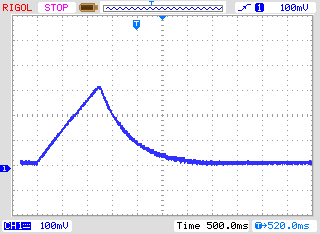
\includegraphics[]{../PNG/charge_15mF.png}
  \caption{Laden und Entladen eines \(15mF\)-Kondensators für die Messung}
  \label{pic:c15mF}
\end{figure}

Nach dieser Kondensatormessung wird die Selbstentladung des Kondensators untersucht, indem der
Spannungsverlust in einer der Ladezeit proportionalen Zeit untersucht wird.
Der gemessene Kapazitätswert wird entsprechend korrigiert. Ein Test mit einer Parallelschaltung von
einem \(68 \mu F\)-Kondensator mit einem \(2.2 k\Omega\)-Widerstand zeigt die
Wirksamkeit der Methode. Der ermittelte Kapazitätswert ohne den Widerstand beträgt \(66.5 \mu F\),
mit dem parallelen \(2.2 k\Omega\) Widerstand wird ein Kapazitätswert von \(65.3 \mu F\) gemessen.
Zum Vergleich möchte ich die entsprechenden Ergebnisse mit einem Peaktech 3315 Multimeter angeben.
Ohne den Widerstand wird eine Kapazität von \(68.2 \mu F\) gemessen, mit dem parallelen \(2.2 k\Omega\)
Widerstand wird aber \(192 \mu F\) mit dem Multimeter gemessen.

\subsection{Messen von kleinen Kapazitäten}
Wenn der erste 10 ms Ladepuls den Kondensator zu hoch aufgeladen hat, wird eine andere Messtechnik benutzt.
Der ATmega-Mikrocontroller hat einen eingebauten 16-Bit-Zähler, der bei voller Taktfrequenz (1MHz oder 8MHz) arbeiten kann.
Diese Zähler hat auch die Fähigkeit aufgrund eines externen Ereignisses den Zählerstand zu sichern.
Dieses Ereignis kann auch das Ausgangs-Signal des Komparators sein.
Der Komparator kann mit jedem ADC-Eingangspin und der Spannungsreferenz (Band Gap Reference) arbeiten.
Das Schaltbild~\ref{fig:comparat} zeigt ein vereinfachtes Diagram der Messsituation.
So entlade ich den Kondensator, bereite den Komparator für den richtigen Pin Eingang vor, starte den Zähler bei 0 und
starte sofort das Laden des Kondensators.
Dabei ist eine Seite des Kondensators mit GND, die andere Seite über den \(470k\Omega\)-Widerstand mit VCC verbunden.
Nun prüfe ich in einer Programm-Schleife, ob der Zähler ein Überlauf-Ereignis (overflow) oder ein
 externes Ereignis (input capture) meldet.
Die Überlauf-Ereignisse zähle ich, bis ich ein externes Ereignis feststelle.
In diesem Fall halte ich den Zähler an und prüfe, ob ich noch einen zusätzlichen Überlauf zählen muss, 
weil der Zähler nicht mit dem externen Ereignis (input capture) angehalten werden kann.


Der Zählerstand des externen Ereignisses bildet zusammen mit dem Überlaufzähler die Gesamtzeit, aus der die
Kapazität mit einem Faktor bestimmt wird.
Die aktuelle Software kann eine Tabelle mit der theoretischen Abhängigkeit der Ladezeit in Bezug auf die gemessene
Komparator-Spannung berücksichtigen.
Die Tabelle besitzt Einträge in Schritten von 50mV, die Ergebnisse werden entsprechend der aktuellen Referenz-Spannung interpoliert.
Diese Tabelle wird nur mit der Makefile Option WITH\_AUTO\_REF aktiviert.
Vom Kapazitätswert ziehe ich eine experimentell herausgefundene vordefinierte Konstante oder eine im Selbsttest
herausgefundene Konstante ab, um den Messwerte-Offset zu beseitigen.
Ich weiß nicht, ob die vordefinierte Konstante für andere Leiterplatten angepasst werden muss.
Mit einem Selbsttest bei gesetzter AUTO\_CAL Option wird diese Anpassung automatisch erledigt.

Ich habe bemerkt, dass die Referenz-Spannung meistens etwas zu klein gemessen wird,
 deshalb kann man einen Zusatz mit der Makefile Option REF\_C\_KORR angeben.
Nach der Kalibration mit der AUTO\_CAL option ist der REF\_C\_KORR Wert nur ein Zusatz zu der automatisch
gefundenen Differenz zwischen geladener Kondensator-Spannung und der internen Referenz-Spannung.
Die gemessene Referenz-Spannung wird dann mit dem Korrekturwert (in mV) korrigiert (addiert).
Wenn die Option WITH\_AUTO\_REF nicht benutzt wird, werden die Referenz-Spannungen entsprechend den Angaben in den
Datenblättern ~\cite{ATmega8}~\cite{ATmega168} der ATmega8, ATmega168 und ATmega328 berücksichtigt.
Eine Beispielmessung von diesem Typ ist in Abbildung~\ref{pic:c22uF} dargestellt.
Die Messzeit für den \(22 \mu F\)-Kondensator beträgt ungefähr 2,6s weil der \(470k\Omega\)-Widerstand für das Laden benutzt wird.
Aber das Entladen geht in diesem Fall viel schneller als das Laden.

\begin{figure}[H]
\centering

\includegraphics[]{../FIG/Comparat.eps}
\caption{Messung kleiner Kapazitätswerte mit dem Komparator}
\label{fig:comparat}
\end{figure}

\begin{figure}[H]
  \centering
    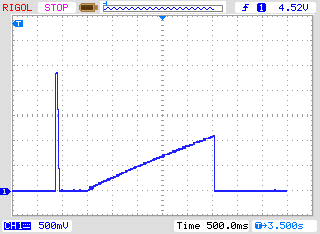
\includegraphics[]{../PNG/charge_22uF.png}
  \caption{Laden und Entladen eines \(22\mu F\)-Kondensators für die Messung}
  \label{pic:c22uF}
\end{figure}


Im Prinzip kann diese Technik auch mit dem \(680\Omega\)-Widerstand benutzt werden,
aber weil während dem Komparatorbetrieb der ADC nicht benutzt werden kann, besteht keine
Möglichkeit die Ladespannung zu beobachten bis der Komparator angehalten wird.
Wenn eine unentdeckte Diode mit dem Kondensator parallelgeschaltet ist, kann der Ladestrom
von der Diode aufgenommen werden (Schwellspannung) und die Referenz-Spannung würde nie erreicht.
Dieser Konzeptfehler wird mit der Methode vermieden, die in der aktuellen Software für große Kondensatoren in Kapitel~\ref{sec:bigcap}
verwendet wird.

\subsection{Messen des äquivalenten Serienwiderstandes ESR, Methode 1}
Der ESR \cite{ESR} stellt zum Beispiel ein Maß für die Alterung von Elektrolyt-Kondensatoren dar.
Die Abbildung~\ref{fig:Cap_equiv} zeigt ein Ersatzschaltbild eines Kondensators.
Der Widerstand \(Rp\) stellt den Isolationswiderstand des Kondensators dar, \(ESL\) die äquivalente
Serieninduktivität und der Widerstand \(ESR\) stellt den äquivalenten Serienwiderstand dar.
Bei Kondensatoren mit mehr als \(0.45 \mu F\) wird versucht, den Serienwiderstand von Kondensatoren zu messen.
Bei mehr als \(3.6 \mu F\) wird dazu die normale Taktrate von \(125 kHz\) für den Analog-Digital Wandler benutzt.
Bei kleineren Kapazitäten wird eine erhöhte Taktrate von \(500 kHz\) benutzt, um die Messung zu beschleunigen.
Die Genauigkeit der ADC-Ergebnisse wird bei der höheren Taktrate zwar schlechter, aber die größeren ESR-Werte
bei kleineren Kondensatoren mildern die Auswirkung dieses Genauigkeitsverlusts ab. 
Andererseits ist sonst nach diesem Verfahren keine ESR-Messung für Kondensatoren unter \(1.8 \mu F\) möglich.

\begin{figure}[H]
  \centering
    
\includegraphics[]{../FIG/Cap_equiv.eps}
  \caption{Ersatzschaltbild eines Kondensators}
  \label{fig:Cap_equiv}
\end{figure}

Genau genommen ist der ESR eines Kondensators abhängig von der Betriebsfrequenz und der Temperatur.
Üblicherweise wird der mit einem sinusförmigen Signal bei \(100 kHz\) gemessene Wert in Datenblättern angegeben.
Bei dieser Frequenz kann der ATmega ohne externe Beschaltung keine Messung durchführen.
Das nachfolgend beschriebene Verfahren erreicht bei der normalen ADC-Taktrate nur eine Messfrequenz von unter 640 Hz
 mit näherungsweise rechteckigem Signal. Bei \(500 kHz\) ADC Taktrate wird etwa 2400 Hz Meßfrequenz erreicht.
Um den äquivalenten Serienwiderstand zu bestimmen,
 wird der Kondensator zuerst in einer Richtung geladen und an beiden Anschlüssen die Spannung mit der internen
Referenzspannung (1.1 V) gemessen.
Nach der Messung wird der Ladestrom abgeschaltet und die Spannung am Kondensator ohne den
Ladestrom gemessen. Wenn die Spannung am Kondensator ohne Ladestrom weniger als 3 mV beträgt, wird
diese Messfolge wiederholt.
Die Abbildung~\ref{fig:Cap_esr} zeigt die entsprechenden Schaltungen.

\begin{figure}[H]
  \centering
    
\includegraphics[]{../FIG/Cap_esr.eps}
  \caption{Schaltbild der ESR-Messung eines Kondensators}
  \label{fig:Cap_esr}
\end{figure}

Die Differenz der Spannung am Kondensator mit und ohne Strom ist ein Maß für den internen Widerstand des Kondensators.
Die zu erwartende Spannungsdifferenz ist allerdings so gering, dass mit einer Messung kein brauchbares Ergebnis erzielt
werden kann.
Aus diesem Grund wird danach der Strom umgekehrt und die Messung in der anderen Richtung wiederholt.
Die gesamte Mess-Sequenz wird 128 Mal durchgeführt und die Ergebnisse der Spannungsmessungen addiert.
Danach hat man drei Spannungssummen, die Spannung \(Ulp\) am Minuspol des Kondensators mit Strom, die Spannung \(Uhp\) am
Pluspol des Kondensators mit Strom und die Spannung \(Uc\) am Pluspol des Kondensators ohne Strom.
Die Spannungssumme am Minuspol des Kondensators repräsentiert den Spannungsabfall bei einem mittleren
Ladestrom am Port-Ausgangswiderstand \(Rport\). Aus der Differenz der Spannungssumme am Pluspol und Minuspol des Kondensators
hat man ein Maß für die Spannung am Kondensator mit Ladestrom \(Udiff = Uhp - Ulp\).
Die Differenz \(Uesr = Udiff - Uc\) soll jetzt den Spannungsabfall bei mittlerem Ladestrom am internen Widerstand des Kondensators
repräsentieren.
Der Widerstandswert wird aus dem Verhältnis dieser Spannung \(Uesr\) zu der Spannung \(Ulp\) skaliert mit dem
bekannten Widerstandwert des Port-Ausgangs \(Rport\). Dabei wird so skaliert, dass eine Widerstandauflösung von
\(0.01 \Omega\) erreicht wird \(Resr = \frac{Uesr \cdot 10 \cdot Rport}{Ulp}\).
Die Abbildung~\ref{pic:esr4} zeigt den Ausschnitt des Spannungsverlaufs eines \(4.2\mu F\) Kondensators
 während der ESR-Messung. Dem Kondensator wurde ein \(6.8 \Omega\) Widerstand in Serie geschaltet, um den ESR Einfluß
zu verdeutlichen. Der kleine Spannungseinbruch nach dem Ladevorgang des Kondensators wird von der Software ausgewertet.
Der größere Spannungseinbruch bei der Messung gegen GND kommt durch den Einfluß des Port-Ausgangswiderstands von etwa \(20 \Omega\) zustande.
Das Ergebnis der ESR-Messung ist in diesem Fall \(7.5 \Omega\), ohne den \(6.8 \Omega\) Widerstand sind es \(0.56 \Omega\).
Die Abbildung~\ref{pic:esr2} zeigt die gleiche Messung mit höherer Meßfrequenz bei einem \(2.2 \mu F\) Elko mit einem ESR von \(6.5 \Omega\).


\begin{figure}[H]
  \begin{subfigure}[b]{9cm}
    \centering
    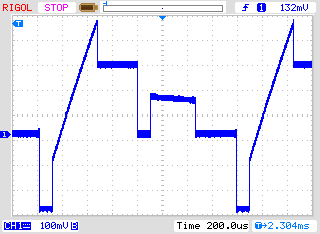
\includegraphics[width=9cm]{../PNG/ESR_4uF.png}
    \caption{Ein Pin gegen GND gemessen}
  \end{subfigure}
  ~
  \begin{subfigure}[b]{9cm}
    \centering
    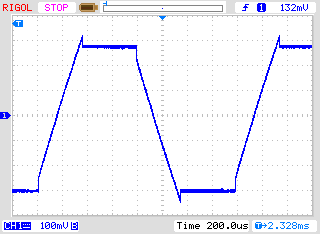
\includegraphics[width=9cm]{../PNG/ESR4uF6R8.png}
    \caption{Von Pin zu Pin gemessen}
  \end{subfigure}
  \caption{Spannungsverlauf eines \(4.2\mu F\) Kondensators während der ESR-Messung}
  \label{pic:esr4}
\end{figure}

\begin{figure}[H]
  \begin{subfigure}[b]{9cm}
    \centering
    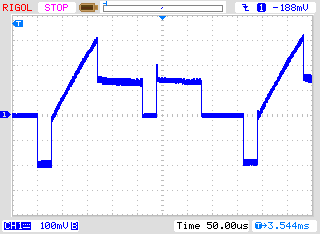
\includegraphics[width=9cm]{../PNG/ESR_2uF_pin2GND.png}
    \caption{Ein Pin gegen GND gemessen}
  \end{subfigure}
  ~
  \begin{subfigure}[b]{9cm}
    \centering
    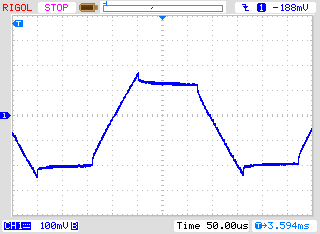
\includegraphics[width=9cm]{../PNG/ESR_2uF_pin2pin.png}
    \caption{Von Pin zu Pin gemessen}
  \end{subfigure}
  \caption{Spannungsverlauf eines \(2.2\mu F\) Kondensators während der ESR-Messung}
  \label{pic:esr2}
\end{figure}

Die Genauigkeit der ESR-Messung ist aus verschiedenen Gründen nicht sehr hoch:
\begin{enumerate}
\item Die Spannungsmessung an den beiden Kondensator-Anschlüssen kann nicht gleichzeitig sondern nur nacheinander durchgeführt werden.
 In der Zwischenzeit hat sich der Ladestrom durch den Ladevorgang des Kondensators geändert.
Dies wird versucht mit einer kapazitätsabhängigen Korrektur der Minuspol-Spannung auszugleichen.
\item Der ADC nimmt den Spannungswert 1,5 Takte nach dem Start des Wandlungsvorgangs. Der Wandelvorgang beginnt mit
der steigenden Flanke des ADC-Taktes, wenn das Startbit gesetzt ist. Wenn der Ladestrom des Kondensators zu früh abgeschaltet wird,
nimmt der ADC die falsche Spannung für die strombehaftete Messung auf. Wird der Ladestrom zu spät abgeschaltet, wird
der Kondensator weiter geladen als es der strombehafteten Messung entspricht.
Dann wird im stromlosen Zustand eine zu hohe Spannung gemessen.
Es ist aber schwierig im Programm den genauen Zeitpunkt für die Stromabschaltung zu treffen.
\item Der Port-Ausgangswiderstand wird bei dieser Messmethode als Referenz benutzt, dessen Widerstandwert
ist aber auch nicht exakt bekannt.
\item Die Auflösung des ADC reicht nicht aus, um eine Widerstandsauflösung von \(0.01 \Omega\) zu erreichen.
Für alle Messungen wird die interne Spannungsreferenz (1.1 V) benutzt, um die best mögliche Auflösung zu verwenden.
Zusätzlich wird versucht, den Auflösungs-Mangel durch eine große Zahl von Einzelmessungen abzumildern.
\item Mit der Abfrage des Fertig-Signals der ADC-Wandlung gelingt es nicht exakt, die Schaltzeiten der Port-Ausgänge mit dem
ADC-Takt zu synchronisieren.
\end{enumerate}

Trotz allen Schwierigkeiten scheinen die Ergebnisse brauchbar zu sein, wie die nachfolgende Abbildung \ref{fig:Cesr} zeigt.
Die ESR-Werte eines Bauteils gemessen mit dem Transistortester schwanken stärker als die Messungen des LCR-meters.
Die Messergebnisse des LCR-Messgerätes wurden bei einer Frequenz von 1 kHz gemessen oder für kleine Kapazitäten auf
2.4 kHz interpoliert.
Beim Transistortester muss auf die Qualität der Anschlüsse geachtet werden. Verwendete Anschlusskabel
erhöhen den gemessenen Widerstandswert. Auch die Kontakte von Steckverbindern können die gemessenen
Widerstandwerte erhöhen. Das LCR-Messgerät macht hier wegen den verwendeten Kelvin-Klemmen weniger Probleme.
Bei den Kondensatoren mit einer Kapazität unter \(1 \mu F\) war ein \(500 nF\) keramischer 
Kondensator (Z5U), alle anderen waren Folien-Kondensatoren. Der einzige Elektrolyt-Kondensator der Meßreihe unter \(9 \mu F\)  
ist ein \(2.2 \mu F\) Kondensator.

\begin{figure}[H]
\centering
% GNUPLOT: LaTeX picture with Postscript
\begingroup
  \makeatletter
  \providecommand\color[2][]{%
    \GenericError{(gnuplot) \space\space\space\@spaces}{%
      Package color not loaded in conjunction with
      terminal option `colourtext'%
    }{See the gnuplot documentation for explanation.%
    }{Either use 'blacktext' in gnuplot or load the package
      color.sty in LaTeX.}%
    \renewcommand\color[2][]{}%
  }%
  \providecommand\includegraphics[2][]{%
    \GenericError{(gnuplot) \space\space\space\@spaces}{%
      Package graphicx or graphics not loaded%
    }{See the gnuplot documentation for explanation.%
    }{The gnuplot epslatex terminal needs graphicx.sty or graphics.sty.}%
    \renewcommand\includegraphics[2][]{}%
  }%
  \providecommand\rotatebox[2]{#2}%
  \@ifundefined{ifGPcolor}{%
    \newif\ifGPcolor
    \GPcolortrue
  }{}%
  \@ifundefined{ifGPblacktext}{%
    \newif\ifGPblacktext
    \GPblacktexttrue
  }{}%
  % define a \g@addto@macro without @ in the name:
  \let\gplgaddtomacro\g@addto@macro
  % define empty templates for all commands taking text:
  \gdef\gplbacktext{}%
  \gdef\gplfronttext{}%
  \makeatother
  \ifGPblacktext
    % no textcolor at all
    \def\colorrgb#1{}%
    \def\colorgray#1{}%
  \else
    % gray or color?
    \ifGPcolor
      \def\colorrgb#1{\color[rgb]{#1}}%
      \def\colorgray#1{\color[gray]{#1}}%
      \expandafter\def\csname LTw\endcsname{\color{white}}%
      \expandafter\def\csname LTb\endcsname{\color{black}}%
      \expandafter\def\csname LTa\endcsname{\color{black}}%
      \expandafter\def\csname LT0\endcsname{\color[rgb]{1,0,0}}%
      \expandafter\def\csname LT1\endcsname{\color[rgb]{0,1,0}}%
      \expandafter\def\csname LT2\endcsname{\color[rgb]{0,0,1}}%
      \expandafter\def\csname LT3\endcsname{\color[rgb]{1,0,1}}%
      \expandafter\def\csname LT4\endcsname{\color[rgb]{0,1,1}}%
      \expandafter\def\csname LT5\endcsname{\color[rgb]{1,1,0}}%
      \expandafter\def\csname LT6\endcsname{\color[rgb]{0,0,0}}%
      \expandafter\def\csname LT7\endcsname{\color[rgb]{1,0.3,0}}%
      \expandafter\def\csname LT8\endcsname{\color[rgb]{0.5,0.5,0.5}}%
    \else
      % gray
      \def\colorrgb#1{\color{black}}%
      \def\colorgray#1{\color[gray]{#1}}%
      \expandafter\def\csname LTw\endcsname{\color{white}}%
      \expandafter\def\csname LTb\endcsname{\color{black}}%
      \expandafter\def\csname LTa\endcsname{\color{black}}%
      \expandafter\def\csname LT0\endcsname{\color{black}}%
      \expandafter\def\csname LT1\endcsname{\color{black}}%
      \expandafter\def\csname LT2\endcsname{\color{black}}%
      \expandafter\def\csname LT3\endcsname{\color{black}}%
      \expandafter\def\csname LT4\endcsname{\color{black}}%
      \expandafter\def\csname LT5\endcsname{\color{black}}%
      \expandafter\def\csname LT6\endcsname{\color{black}}%
      \expandafter\def\csname LT7\endcsname{\color{black}}%
      \expandafter\def\csname LT8\endcsname{\color{black}}%
    \fi
  \fi
  \setlength{\unitlength}{0.0500bp}%
  \begin{picture}(7200.00,5040.00)%
    \gplgaddtomacro\gplbacktext{%
      \csname LTb\endcsname%
      \put(946,704){\makebox(0,0)[r]{\strut{} 0}}%
      \csname LTb\endcsname%
      \put(946,1383){\makebox(0,0)[r]{\strut{} 0.2}}%
      \csname LTb\endcsname%
      \put(946,2061){\makebox(0,0)[r]{\strut{} 0.4}}%
      \csname LTb\endcsname%
      \put(946,2740){\makebox(0,0)[r]{\strut{} 0.6}}%
      \csname LTb\endcsname%
      \put(946,3418){\makebox(0,0)[r]{\strut{} 0.8}}%
      \csname LTb\endcsname%
      \put(946,4097){\makebox(0,0)[r]{\strut{} 1}}%
      \csname LTb\endcsname%
      \put(946,4775){\makebox(0,0)[r]{\strut{} 1.2}}%
      \csname LTb\endcsname%
      \put(1078,484){\makebox(0,0){\strut{}1u}}%
      \csname LTb\endcsname%
      \put(2986,484){\makebox(0,0){\strut{}10u}}%
      \csname LTb\endcsname%
      \put(4895,484){\makebox(0,0){\strut{}100u}}%
      \csname LTb\endcsname%
      \put(6803,484){\makebox(0,0){\strut{}1m}}%
      \put(176,2739){\rotatebox{-270}{\makebox(0,0){\strut{}ESR / Ohm}}}%
      \put(3940,154){\makebox(0,0){\strut{}Capacity value / F}}%
      \put(3940,4665){\makebox(0,0){\strut{}}}%
    }%
    \gplgaddtomacro\gplfronttext{%
      \csname LTb\endcsname%
      \put(5690,4594){\makebox(0,0)[r]{\strut{}328p}}%
      \csname LTb\endcsname%
      \put(5690,4358){\makebox(0,0)[r]{\strut{}328}}%
      \csname LTb\endcsname%
      \put(5690,4122){\makebox(0,0)[r]{\strut{}168p}}%
      \csname LTb\endcsname%
      \put(5690,3886){\makebox(0,0)[r]{\strut{}168a}}%
      \csname LTb\endcsname%
      \put(5690,3650){\makebox(0,0)[r]{\strut{}168}}%
      \csname LTb\endcsname%
      \put(5690,3414){\makebox(0,0)[r]{\strut{}LCR}}%
    }%
    \gplbacktext
    \put(0,0){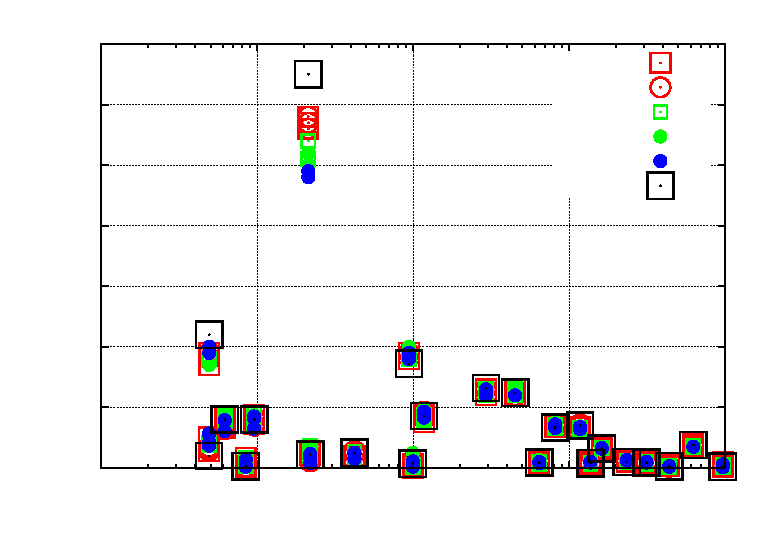
\includegraphics{../GNU/Cesr}}%
    \gplfronttext
  \end{picture}%
\endgroup

\caption{Messergebnisse der ESR-Messungen mit 15 veschiedenen ATmega}
\label{fig:Cesr}
\end{figure}

\newpage
\subsection{Messen des äquivalenten Serienwiderstandes ESR, Methode 2}
Ab der Softwareversion 1.07k wurde die ESR-Messung auf eine modifizierte Meßmethode umgestellt.
Die einzelnen Meßschritte sind in Abbildung~\ref{fig:Cap_esr2} gezeigt. Das besondere an der Methode
ist, daß die Zeit des Stromflusses durch den Kondensator wesentlich gegenüber der Methode 1 verringert wurde.
Der Kondensator wird mit einem Puls der halben Breite negativ vorgeladen und wird dann zyklisch aufgeladen und in der
Gegenrichtung wieder entladen.
Dabei wird der Ladepuls zeitlich so gelegt, daß bei Sample 4 und 8 zur Pulsmitte
die Spannung für den ADC abgegriffen wird (Sample and Hold, 2.5 ADC Takte nach dem Start).
Ein kompletter Meßzyklus wird in Abbildung~\ref{fig:Cap_esr2_timing} gezeigt.
Es werden auch bei dieser Meßmethode die Summen der Meßergebnisse aus 255 Zyklen ausgewertet,
um eine ausreichende Auflösung zu erreichen.
Eine fortlaufende Aufladung des Kondensators in die eine oder andere Richtung wird durch die kurzen und
gleich langen Auflade- und Entlade-Pulse bei gleicher Beschaltung weitgehend vermieden.
Bei der Messung der Referenzspannung fließt kein Strom durch den Kondensator. Dadurch ist diese Messung
nicht zeitkritisch. Es wird lediglich vorausgesetzt, daß der Kondensator seine Spannung in der
stromlosen Zeit beibehält.

\begin{figure}[H]
  \centering
    
\includegraphics[width=18cm]{../FIG/Cap_esr2_timing.eps}
  \caption{Zeitlicher Ablauf eines Meßzyklus der neuen ESR-Messung}
  \label{fig:Cap_esr2_timing}
\end{figure}

\begin{figure}[H]
  \centering
    
\includegraphics[]{../FIG/Cap_esr2.eps}
  \caption{Vereinfachte ESR-Messung eines Kondensators}
  \label{fig:Cap_esr2}
\end{figure}


Durch den kürzeren Ladepuls kann nicht nur der ESR von geringeren Kapazitätswerten gemessen werden, sondern
diese Methode kann auch für die Messung kleiner Widerstandswerte benutzt werden, wenn die Widerstände
keine meßbare Induktivität besitzen. Dadurch kann die Auflösung bei Widerstandswerten unter \(10 \Omega\) auf 
\(0.01 \Omega\) gesenkt werden. Daneben kann auch der Nullwiderstand für die Widerstandsmessung als auch
für die ESR-Messung im Selbsttestzweig der Kalibration für alle drei Testpin-Kombinationen bestimmt werden.
Auf solide Steckverbindungen oder Klemmverbindungen sollte für stabile Ergebnisse geachtet werden.
Die Meßperiode beträgt etwa \(900 \mu s\), was einer Frequenz von etwa \(1.1 kHz\) entspricht.
Wegen der Kürze der Ladepulse entspricht das Ergebnis aber eher einer Messung mit \(10 kHz\).
Als Beispiel wird die Messung eines \(10 \mu F\) Folienkondensators einmal direkt und einmal mit einem
\(2.7 \Omega\) Serienwiderstand in Abbildung~\ref{pic:NewEsr10} gezeigt.
Deutlich kann man den Einfluß des zusätzlichen Widerstandes beim Vergleich der beiden Diagramme erkennen.
Hier wird auch verständlich, warum die ADC-Messung in der Mitte des Ladepulses erfolgen muß.
Bei großen Kondensatoren bleibt der Ladestrom des Kondensators hinreichend gut konstant,
so daß bei der zeitlichen Mitte des Ladepulses auch die mittlere Spannung gemessen wird.
Bei keineren Kondensatoren ergibt sich ein deutlicherer Unterschied, der aber mit dem
bekannten Kapazitätswert relativ gut kompensiert werden kann.

\begin{figure}[H]
  \begin{subfigure}[b]{9cm}
    \centering
    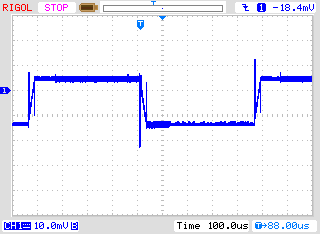
\includegraphics[width=9cm]{../PNG/NewEsr10uF0R0.png}
    \caption{ohne Serienwiderstand}
  \end{subfigure}
  ~
  \begin{subfigure}[b]{9cm}
    \centering
    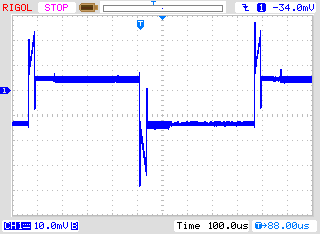
\includegraphics[width=9cm]{../PNG/NewEsr10uF2R7.png}
    \caption{mit \(2.7\Omega\) Serienwiderstand}
  \end{subfigure}
  \caption{Spannungsverlauf eines \(10\mu F\) Kondensators während der neuen ESR-Messung}
  \label{pic:NewEsr10}
\end{figure}

Die Meßergebnisse der neuen ESR-Meßmethode sind in Abbildung~\ref{fig:Cesr2} dargestellt.
Die ESR-Werte unterscheiden sich wegen der Frequenzabhängigkeit von den Ergebnissen der Abbildung~\ref{fig:Cesr}.
Die Vergleichswerte des LCR-Meßgerätes sind bei \(10 kHz\) ermittelt worden.

\begin{figure}[H]
\centering
% GNUPLOT: LaTeX picture with Postscript
\begingroup
  \makeatletter
  \providecommand\color[2][]{%
    \GenericError{(gnuplot) \space\space\space\@spaces}{%
      Package color not loaded in conjunction with
      terminal option `colourtext'%
    }{See the gnuplot documentation for explanation.%
    }{Either use 'blacktext' in gnuplot or load the package
      color.sty in LaTeX.}%
    \renewcommand\color[2][]{}%
  }%
  \providecommand\includegraphics[2][]{%
    \GenericError{(gnuplot) \space\space\space\@spaces}{%
      Package graphicx or graphics not loaded%
    }{See the gnuplot documentation for explanation.%
    }{The gnuplot epslatex terminal needs graphicx.sty or graphics.sty.}%
    \renewcommand\includegraphics[2][]{}%
  }%
  \providecommand\rotatebox[2]{#2}%
  \@ifundefined{ifGPcolor}{%
    \newif\ifGPcolor
    \GPcolortrue
  }{}%
  \@ifundefined{ifGPblacktext}{%
    \newif\ifGPblacktext
    \GPblacktexttrue
  }{}%
  % define a \g@addto@macro without @ in the name:
  \let\gplgaddtomacro\g@addto@macro
  % define empty templates for all commands taking text:
  \gdef\gplbacktext{}%
  \gdef\gplfronttext{}%
  \makeatother
  \ifGPblacktext
    % no textcolor at all
    \def\colorrgb#1{}%
    \def\colorgray#1{}%
  \else
    % gray or color?
    \ifGPcolor
      \def\colorrgb#1{\color[rgb]{#1}}%
      \def\colorgray#1{\color[gray]{#1}}%
      \expandafter\def\csname LTw\endcsname{\color{white}}%
      \expandafter\def\csname LTb\endcsname{\color{black}}%
      \expandafter\def\csname LTa\endcsname{\color{black}}%
      \expandafter\def\csname LT0\endcsname{\color[rgb]{1,0,0}}%
      \expandafter\def\csname LT1\endcsname{\color[rgb]{0,1,0}}%
      \expandafter\def\csname LT2\endcsname{\color[rgb]{0,0,1}}%
      \expandafter\def\csname LT3\endcsname{\color[rgb]{1,0,1}}%
      \expandafter\def\csname LT4\endcsname{\color[rgb]{0,1,1}}%
      \expandafter\def\csname LT5\endcsname{\color[rgb]{1,1,0}}%
      \expandafter\def\csname LT6\endcsname{\color[rgb]{0,0,0}}%
      \expandafter\def\csname LT7\endcsname{\color[rgb]{1,0.3,0}}%
      \expandafter\def\csname LT8\endcsname{\color[rgb]{0.5,0.5,0.5}}%
    \else
      % gray
      \def\colorrgb#1{\color{black}}%
      \def\colorgray#1{\color[gray]{#1}}%
      \expandafter\def\csname LTw\endcsname{\color{white}}%
      \expandafter\def\csname LTb\endcsname{\color{black}}%
      \expandafter\def\csname LTa\endcsname{\color{black}}%
      \expandafter\def\csname LT0\endcsname{\color{black}}%
      \expandafter\def\csname LT1\endcsname{\color{black}}%
      \expandafter\def\csname LT2\endcsname{\color{black}}%
      \expandafter\def\csname LT3\endcsname{\color{black}}%
      \expandafter\def\csname LT4\endcsname{\color{black}}%
      \expandafter\def\csname LT5\endcsname{\color{black}}%
      \expandafter\def\csname LT6\endcsname{\color{black}}%
      \expandafter\def\csname LT7\endcsname{\color{black}}%
      \expandafter\def\csname LT8\endcsname{\color{black}}%
    \fi
  \fi
  \setlength{\unitlength}{0.0500bp}%
  \begin{picture}(7200.00,5040.00)%
    \gplgaddtomacro\gplbacktext{%
      \csname LTb\endcsname%
      \put(1078,704){\makebox(0,0)[r]{\strut{} 0.01}}%
      \csname LTb\endcsname%
      \put(1078,2061){\makebox(0,0)[r]{\strut{} 0.1}}%
      \csname LTb\endcsname%
      \put(1078,3418){\makebox(0,0)[r]{\strut{} 1}}%
      \csname LTb\endcsname%
      \put(1078,4775){\makebox(0,0)[r]{\strut{} 10}}%
      \csname LTb\endcsname%
      \put(1210,484){\makebox(0,0){\strut{}100n}}%
      \csname LTb\endcsname%
      \put(2608,484){\makebox(0,0){\strut{}1u}}%
      \csname LTb\endcsname%
      \put(4007,484){\makebox(0,0){\strut{}10u}}%
      \csname LTb\endcsname%
      \put(5405,484){\makebox(0,0){\strut{}100u}}%
      \csname LTb\endcsname%
      \put(6803,484){\makebox(0,0){\strut{}1m}}%
      \put(176,2739){\rotatebox{-270}{\makebox(0,0){\strut{}ESR / Ohm}}}%
      \put(4006,154){\makebox(0,0){\strut{}Capacity value / F}}%
      \put(4006,4665){\makebox(0,0){\strut{}}}%
    }%
    \gplgaddtomacro\gplfronttext{%
      \csname LTb\endcsname%
      \put(5690,4594){\makebox(0,0)[r]{\strut{}328p}}%
      \csname LTb\endcsname%
      \put(5690,4358){\makebox(0,0)[r]{\strut{}328}}%
      \csname LTb\endcsname%
      \put(5690,4122){\makebox(0,0)[r]{\strut{}168p}}%
      \csname LTb\endcsname%
      \put(5690,3886){\makebox(0,0)[r]{\strut{}168a}}%
      \csname LTb\endcsname%
      \put(5690,3650){\makebox(0,0)[r]{\strut{}168}}%
      \csname LTb\endcsname%
      \put(5690,3414){\makebox(0,0)[r]{\strut{}LCR}}%
    }%
    \gplbacktext
    \put(0,0){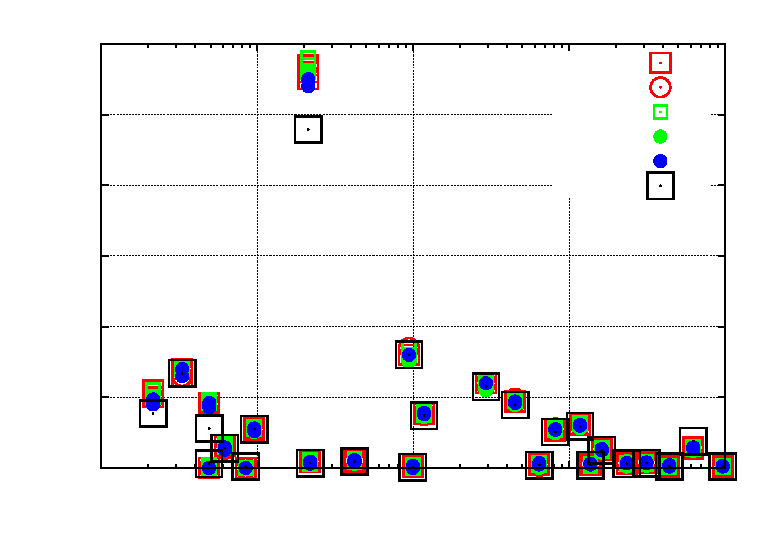
\includegraphics{../GNU/Cesr2}}%
    \gplfronttext
  \end{picture}%
\endgroup

\caption{Messergebnisse der ESR-Messungen mit 15 veschiedenen ATmega, Methode 2}
\label{fig:Cesr2}
\end{figure}


\subsection{Spannungsverlust nach einem Ladepuls, Vloss}
Beim Meßverfahren von großen Kapazitäten wird der Spannungsverlust nach einem Ladepuls im stromlosen Zustand untersucht.
Die erreichte Ladespannung sinkt bei Elektrolyt-Kondensatoren nach kurzer Zeit wieder etwas ab.
Dieser Spannungsverlust kann durch einen parallel geschalteten Widerstand verursacht werden.
Ich nehme an, daß der Spannungsverlust bei Elektrolyt-Kondensatoren durch eine interne Ladungsverteilung nach
dem Ladepuls verursacht wird. Bei einem langsamen Ladevorgang, wie er bei kleineren Kapazitäten mit dem \(470 k\Omega\) Widerstand
gemacht wird, ist diese Umverteilung schon während des Ladevorgangs abgeschlossen. Dann tritt kein meßbarer Spannungsverlust nach
der Ladung in der betrachteten Zeitspanne auf. Wird der gleiche Elektrolyt-Kondensator aber mit einem
kurzem pulsförmigen Strom geladen, ist hier auch ein Spannungsverlust durch die nachträgliche Umverteilung
der Ladung zu beobachten. Der gleiche Effekt ist in geringerem Umfang auch bei keramischen Kondensatoren zu beobachten. 
Nach den bisherigen Beobachtungen sind Kondensatoren mit mehreren \% Spannungsverlust verdächtig.

\subsection{Ergebnisse der Kondensator-Messung}
Die Ergebnisse meiner Messungen werden in Abbildung~\ref{fig:mega8cap} für drei ATmega8 dargestellt.
Zusätzlich sind einige Werte der Original-Software mit einem Korrekturfaktor
von 0,88~(-12\%) dargestellt.
Weitere Ergebnisse von ATmega8 Versionen zeigen die Abbildungen~\ref{fig:mega8Acap} und \ref{fig:mega8Lcap}.
Die Ergebnisse der Messung der gleichen Kondensatoren mit einem ATmega168 werden in Abbildung~\ref{fig:mega168cap} gezeigt.
Die Referenz für die Fehlerberechnung sind die Messwerte eines PeakTech 2170 LCR-Messgerätes, 
 nicht die aufgedruckten Werte der Bauteile.
Die grösseren relativen Messfehler bei großen Kondensatoren liegen zum Teil an der zu hohen Messfrequenz (100 Hz) des
LCR-Messgerätes für große Elektrolytkondensatoren, zum anderen spielt auch die schlechte Güte der
Elektrolytkondensatoren eine Rolle.

\begin{figure}[H]
\centering
% GNUPLOT: LaTeX picture with Postscript
\begingroup
  \makeatletter
  \providecommand\color[2][]{%
    \GenericError{(gnuplot) \space\space\space\@spaces}{%
      Package color not loaded in conjunction with
      terminal option `colourtext'%
    }{See the gnuplot documentation for explanation.%
    }{Either use 'blacktext' in gnuplot or load the package
      color.sty in LaTeX.}%
    \renewcommand\color[2][]{}%
  }%
  \providecommand\includegraphics[2][]{%
    \GenericError{(gnuplot) \space\space\space\@spaces}{%
      Package graphicx or graphics not loaded%
    }{See the gnuplot documentation for explanation.%
    }{The gnuplot epslatex terminal needs graphicx.sty or graphics.sty.}%
    \renewcommand\includegraphics[2][]{}%
  }%
  \providecommand\rotatebox[2]{#2}%
  \@ifundefined{ifGPcolor}{%
    \newif\ifGPcolor
    \GPcolortrue
  }{}%
  \@ifundefined{ifGPblacktext}{%
    \newif\ifGPblacktext
    \GPblacktexttrue
  }{}%
  % define a \g@addto@macro without @ in the name:
  \let\gplgaddtomacro\g@addto@macro
  % define empty templates for all commands taking text:
  \gdef\gplbacktext{}%
  \gdef\gplfronttext{}%
  \makeatother
  \ifGPblacktext
    % no textcolor at all
    \def\colorrgb#1{}%
    \def\colorgray#1{}%
  \else
    % gray or color?
    \ifGPcolor
      \def\colorrgb#1{\color[rgb]{#1}}%
      \def\colorgray#1{\color[gray]{#1}}%
      \expandafter\def\csname LTw\endcsname{\color{white}}%
      \expandafter\def\csname LTb\endcsname{\color{black}}%
      \expandafter\def\csname LTa\endcsname{\color{black}}%
      \expandafter\def\csname LT0\endcsname{\color[rgb]{1,0,0}}%
      \expandafter\def\csname LT1\endcsname{\color[rgb]{0,1,0}}%
      \expandafter\def\csname LT2\endcsname{\color[rgb]{0,0,1}}%
      \expandafter\def\csname LT3\endcsname{\color[rgb]{1,0,1}}%
      \expandafter\def\csname LT4\endcsname{\color[rgb]{0,1,1}}%
      \expandafter\def\csname LT5\endcsname{\color[rgb]{1,1,0}}%
      \expandafter\def\csname LT6\endcsname{\color[rgb]{0,0,0}}%
      \expandafter\def\csname LT7\endcsname{\color[rgb]{1,0.3,0}}%
      \expandafter\def\csname LT8\endcsname{\color[rgb]{0.5,0.5,0.5}}%
    \else
      % gray
      \def\colorrgb#1{\color{black}}%
      \def\colorgray#1{\color[gray]{#1}}%
      \expandafter\def\csname LTw\endcsname{\color{white}}%
      \expandafter\def\csname LTb\endcsname{\color{black}}%
      \expandafter\def\csname LTa\endcsname{\color{black}}%
      \expandafter\def\csname LT0\endcsname{\color{black}}%
      \expandafter\def\csname LT1\endcsname{\color{black}}%
      \expandafter\def\csname LT2\endcsname{\color{black}}%
      \expandafter\def\csname LT3\endcsname{\color{black}}%
      \expandafter\def\csname LT4\endcsname{\color{black}}%
      \expandafter\def\csname LT5\endcsname{\color{black}}%
      \expandafter\def\csname LT6\endcsname{\color{black}}%
      \expandafter\def\csname LT7\endcsname{\color{black}}%
      \expandafter\def\csname LT8\endcsname{\color{black}}%
    \fi
  \fi
  \setlength{\unitlength}{0.0500bp}%
  \begin{picture}(7200.00,5040.00)%
    \gplgaddtomacro\gplbacktext{%
      \csname LTb\endcsname%
      \put(814,704){\makebox(0,0)[r]{\strut{}-10}}%
      \csname LTb\endcsname%
      \put(814,1213){\makebox(0,0)[r]{\strut{}-5}}%
      \csname LTb\endcsname%
      \put(814,1722){\makebox(0,0)[r]{\strut{} 0}}%
      \csname LTb\endcsname%
      \put(814,2231){\makebox(0,0)[r]{\strut{} 5}}%
      \csname LTb\endcsname%
      \put(814,2740){\makebox(0,0)[r]{\strut{} 10}}%
      \csname LTb\endcsname%
      \put(814,3248){\makebox(0,0)[r]{\strut{} 15}}%
      \csname LTb\endcsname%
      \put(814,3757){\makebox(0,0)[r]{\strut{} 20}}%
      \csname LTb\endcsname%
      \put(814,4266){\makebox(0,0)[r]{\strut{} 25}}%
      \csname LTb\endcsname%
      \put(814,4775){\makebox(0,0)[r]{\strut{} 30}}%
      \csname LTb\endcsname%
      \put(946,484){\makebox(0,0){\strut{}10p}}%
      \csname LTb\endcsname%
      \put(1532,484){\makebox(0,0){\strut{}100p}}%
      \csname LTb\endcsname%
      \put(2117,484){\makebox(0,0){\strut{}1n}}%
      \csname LTb\endcsname%
      \put(2703,484){\makebox(0,0){\strut{}10n}}%
      \csname LTb\endcsname%
      \put(3289,484){\makebox(0,0){\strut{}100n}}%
      \csname LTb\endcsname%
      \put(3875,484){\makebox(0,0){\strut{}1u}}%
      \csname LTb\endcsname%
      \put(4460,484){\makebox(0,0){\strut{}10u}}%
      \csname LTb\endcsname%
      \put(5046,484){\makebox(0,0){\strut{}100u}}%
      \csname LTb\endcsname%
      \put(5632,484){\makebox(0,0){\strut{}1m}}%
      \csname LTb\endcsname%
      \put(6217,484){\makebox(0,0){\strut{}10m}}%
      \csname LTb\endcsname%
      \put(6803,484){\makebox(0,0){\strut{}100m}}%
      \put(176,2739){\rotatebox{-270}{\makebox(0,0){\strut{}Error / Percent}}}%
      \put(3874,154){\makebox(0,0){\strut{}Capacity value / F}}%
      \put(3874,4665){\makebox(0,0){\strut{}}}%
    }%
    \gplgaddtomacro\gplfronttext{%
      \csname LTb\endcsname%
      \put(2002,4602){\makebox(0,0)[r]{\strut{}Mega8}}%
      \csname LTb\endcsname%
      \put(2002,4382){\makebox(0,0)[r]{\strut{}Mega8as}}%
      \csname LTb\endcsname%
      \put(2002,4162){\makebox(0,0)[r]{\strut{}orig}}%
    }%
    \gplbacktext
    \put(0,0){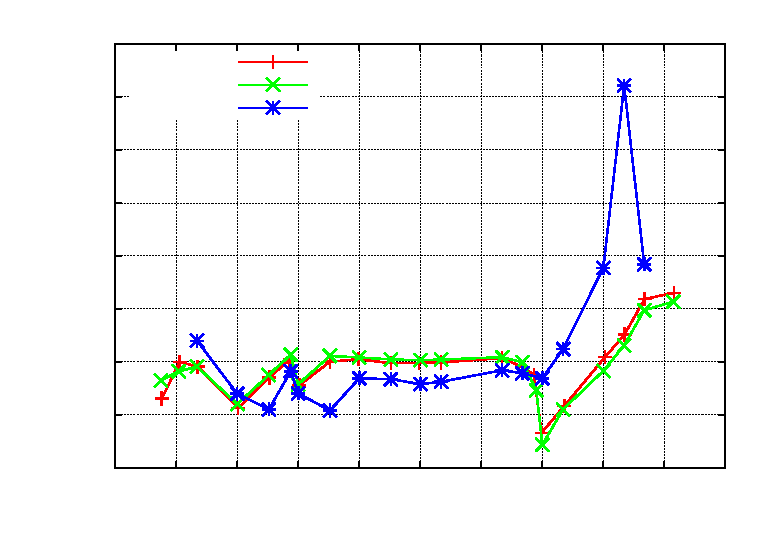
\includegraphics{../GNU/Mega8cap}}%
    \gplfronttext
  \end{picture}%
\endgroup

\caption{Prozentualer Fehler der Kondensator-Messungen mit drei ATmega8}
\label{fig:mega8cap}
\end{figure}

\begin{figure}[H]
  \begin{subfigure}[b]{9cm}
    \centering
    \resizebox{9cm}{!}{% GNUPLOT: LaTeX picture with Postscript
\begingroup
  \makeatletter
  \providecommand\color[2][]{%
    \GenericError{(gnuplot) \space\space\space\@spaces}{%
      Package color not loaded in conjunction with
      terminal option `colourtext'%
    }{See the gnuplot documentation for explanation.%
    }{Either use 'blacktext' in gnuplot or load the package
      color.sty in LaTeX.}%
    \renewcommand\color[2][]{}%
  }%
  \providecommand\includegraphics[2][]{%
    \GenericError{(gnuplot) \space\space\space\@spaces}{%
      Package graphicx or graphics not loaded%
    }{See the gnuplot documentation for explanation.%
    }{The gnuplot epslatex terminal needs graphicx.sty or graphics.sty.}%
    \renewcommand\includegraphics[2][]{}%
  }%
  \providecommand\rotatebox[2]{#2}%
  \@ifundefined{ifGPcolor}{%
    \newif\ifGPcolor
    \GPcolortrue
  }{}%
  \@ifundefined{ifGPblacktext}{%
    \newif\ifGPblacktext
    \GPblacktexttrue
  }{}%
  % define a \g@addto@macro without @ in the name:
  \let\gplgaddtomacro\g@addto@macro
  % define empty templates for all commands taking text:
  \gdef\gplbacktext{}%
  \gdef\gplfronttext{}%
  \makeatother
  \ifGPblacktext
    % no textcolor at all
    \def\colorrgb#1{}%
    \def\colorgray#1{}%
  \else
    % gray or color?
    \ifGPcolor
      \def\colorrgb#1{\color[rgb]{#1}}%
      \def\colorgray#1{\color[gray]{#1}}%
      \expandafter\def\csname LTw\endcsname{\color{white}}%
      \expandafter\def\csname LTb\endcsname{\color{black}}%
      \expandafter\def\csname LTa\endcsname{\color{black}}%
      \expandafter\def\csname LT0\endcsname{\color[rgb]{1,0,0}}%
      \expandafter\def\csname LT1\endcsname{\color[rgb]{0,1,0}}%
      \expandafter\def\csname LT2\endcsname{\color[rgb]{0,0,1}}%
      \expandafter\def\csname LT3\endcsname{\color[rgb]{1,0,1}}%
      \expandafter\def\csname LT4\endcsname{\color[rgb]{0,1,1}}%
      \expandafter\def\csname LT5\endcsname{\color[rgb]{1,1,0}}%
      \expandafter\def\csname LT6\endcsname{\color[rgb]{0,0,0}}%
      \expandafter\def\csname LT7\endcsname{\color[rgb]{1,0.3,0}}%
      \expandafter\def\csname LT8\endcsname{\color[rgb]{0.5,0.5,0.5}}%
    \else
      % gray
      \def\colorrgb#1{\color{black}}%
      \def\colorgray#1{\color[gray]{#1}}%
      \expandafter\def\csname LTw\endcsname{\color{white}}%
      \expandafter\def\csname LTb\endcsname{\color{black}}%
      \expandafter\def\csname LTa\endcsname{\color{black}}%
      \expandafter\def\csname LT0\endcsname{\color{black}}%
      \expandafter\def\csname LT1\endcsname{\color{black}}%
      \expandafter\def\csname LT2\endcsname{\color{black}}%
      \expandafter\def\csname LT3\endcsname{\color{black}}%
      \expandafter\def\csname LT4\endcsname{\color{black}}%
      \expandafter\def\csname LT5\endcsname{\color{black}}%
      \expandafter\def\csname LT6\endcsname{\color{black}}%
      \expandafter\def\csname LT7\endcsname{\color{black}}%
      \expandafter\def\csname LT8\endcsname{\color{black}}%
    \fi
  \fi
  \setlength{\unitlength}{0.0500bp}%
  \begin{picture}(7200.00,5040.00)%
    \gplgaddtomacro\gplbacktext{%
      \csname LTb\endcsname%
      \put(814,704){\makebox(0,0)[r]{\strut{}-2}}%
      \csname LTb\endcsname%
      \put(814,1383){\makebox(0,0)[r]{\strut{} 0}}%
      \csname LTb\endcsname%
      \put(814,2061){\makebox(0,0)[r]{\strut{} 2}}%
      \csname LTb\endcsname%
      \put(814,2740){\makebox(0,0)[r]{\strut{} 4}}%
      \csname LTb\endcsname%
      \put(814,3418){\makebox(0,0)[r]{\strut{} 6}}%
      \csname LTb\endcsname%
      \put(814,4097){\makebox(0,0)[r]{\strut{} 8}}%
      \csname LTb\endcsname%
      \put(814,4775){\makebox(0,0)[r]{\strut{} 10}}%
      \csname LTb\endcsname%
      \put(946,484){\makebox(0,0){\strut{}10p}}%
      \csname LTb\endcsname%
      \put(1532,484){\makebox(0,0){\strut{}100p}}%
      \csname LTb\endcsname%
      \put(2117,484){\makebox(0,0){\strut{}1n}}%
      \csname LTb\endcsname%
      \put(2703,484){\makebox(0,0){\strut{}10n}}%
      \csname LTb\endcsname%
      \put(3289,484){\makebox(0,0){\strut{}100n}}%
      \csname LTb\endcsname%
      \put(3875,484){\makebox(0,0){\strut{}1u}}%
      \csname LTb\endcsname%
      \put(4460,484){\makebox(0,0){\strut{}10u}}%
      \csname LTb\endcsname%
      \put(5046,484){\makebox(0,0){\strut{}100u}}%
      \csname LTb\endcsname%
      \put(5632,484){\makebox(0,0){\strut{}1m}}%
      \csname LTb\endcsname%
      \put(6217,484){\makebox(0,0){\strut{}10m}}%
      \csname LTb\endcsname%
      \put(6803,484){\makebox(0,0){\strut{}100m}}%
      \put(176,2739){\rotatebox{-270}{\makebox(0,0){\strut{}Error / Percent}}}%
      \put(3874,154){\makebox(0,0){\strut{}Capacity value / F}}%
      \put(3874,4665){\makebox(0,0){\strut{}}}%
    }%
    \gplgaddtomacro\gplfronttext{%
      \csname LTb\endcsname%
      \put(2134,4602){\makebox(0,0)[r]{\strut{}Mega8A-4}}%
      \csname LTb\endcsname%
      \put(2134,4382){\makebox(0,0)[r]{\strut{}Mega8A-5}}%
      \csname LTb\endcsname%
      \put(2134,4162){\makebox(0,0)[r]{\strut{}Mega8A-6}}%
    }%
    \gplbacktext
    \put(0,0){\includegraphics{../GNU/Mega8Acap}}%
    \gplfronttext
  \end{picture}%
\endgroup
}
    \caption{mit drei ATmega8A}
    \label{fig:mega8Acap}
  \end{subfigure}
  ~
  \begin{subfigure}[b]{9cm}
    \centering
    \resizebox{9cm}{!}{% GNUPLOT: LaTeX picture with Postscript
\begingroup
  \makeatletter
  \providecommand\color[2][]{%
    \GenericError{(gnuplot) \space\space\space\@spaces}{%
      Package color not loaded in conjunction with
      terminal option `colourtext'%
    }{See the gnuplot documentation for explanation.%
    }{Either use 'blacktext' in gnuplot or load the package
      color.sty in LaTeX.}%
    \renewcommand\color[2][]{}%
  }%
  \providecommand\includegraphics[2][]{%
    \GenericError{(gnuplot) \space\space\space\@spaces}{%
      Package graphicx or graphics not loaded%
    }{See the gnuplot documentation for explanation.%
    }{The gnuplot epslatex terminal needs graphicx.sty or graphics.sty.}%
    \renewcommand\includegraphics[2][]{}%
  }%
  \providecommand\rotatebox[2]{#2}%
  \@ifundefined{ifGPcolor}{%
    \newif\ifGPcolor
    \GPcolortrue
  }{}%
  \@ifundefined{ifGPblacktext}{%
    \newif\ifGPblacktext
    \GPblacktexttrue
  }{}%
  % define a \g@addto@macro without @ in the name:
  \let\gplgaddtomacro\g@addto@macro
  % define empty templates for all commands taking text:
  \gdef\gplbacktext{}%
  \gdef\gplfronttext{}%
  \makeatother
  \ifGPblacktext
    % no textcolor at all
    \def\colorrgb#1{}%
    \def\colorgray#1{}%
  \else
    % gray or color?
    \ifGPcolor
      \def\colorrgb#1{\color[rgb]{#1}}%
      \def\colorgray#1{\color[gray]{#1}}%
      \expandafter\def\csname LTw\endcsname{\color{white}}%
      \expandafter\def\csname LTb\endcsname{\color{black}}%
      \expandafter\def\csname LTa\endcsname{\color{black}}%
      \expandafter\def\csname LT0\endcsname{\color[rgb]{1,0,0}}%
      \expandafter\def\csname LT1\endcsname{\color[rgb]{0,1,0}}%
      \expandafter\def\csname LT2\endcsname{\color[rgb]{0,0,1}}%
      \expandafter\def\csname LT3\endcsname{\color[rgb]{1,0,1}}%
      \expandafter\def\csname LT4\endcsname{\color[rgb]{0,1,1}}%
      \expandafter\def\csname LT5\endcsname{\color[rgb]{1,1,0}}%
      \expandafter\def\csname LT6\endcsname{\color[rgb]{0,0,0}}%
      \expandafter\def\csname LT7\endcsname{\color[rgb]{1,0.3,0}}%
      \expandafter\def\csname LT8\endcsname{\color[rgb]{0.5,0.5,0.5}}%
    \else
      % gray
      \def\colorrgb#1{\color{black}}%
      \def\colorgray#1{\color[gray]{#1}}%
      \expandafter\def\csname LTw\endcsname{\color{white}}%
      \expandafter\def\csname LTb\endcsname{\color{black}}%
      \expandafter\def\csname LTa\endcsname{\color{black}}%
      \expandafter\def\csname LT0\endcsname{\color{black}}%
      \expandafter\def\csname LT1\endcsname{\color{black}}%
      \expandafter\def\csname LT2\endcsname{\color{black}}%
      \expandafter\def\csname LT3\endcsname{\color{black}}%
      \expandafter\def\csname LT4\endcsname{\color{black}}%
      \expandafter\def\csname LT5\endcsname{\color{black}}%
      \expandafter\def\csname LT6\endcsname{\color{black}}%
      \expandafter\def\csname LT7\endcsname{\color{black}}%
      \expandafter\def\csname LT8\endcsname{\color{black}}%
    \fi
  \fi
  \setlength{\unitlength}{0.0500bp}%
  \begin{picture}(7200.00,5040.00)%
    \gplgaddtomacro\gplbacktext{%
      \csname LTb\endcsname%
      \put(814,704){\makebox(0,0)[r]{\strut{}-2}}%
      \csname LTb\endcsname%
      \put(814,1383){\makebox(0,0)[r]{\strut{} 0}}%
      \csname LTb\endcsname%
      \put(814,2061){\makebox(0,0)[r]{\strut{} 2}}%
      \csname LTb\endcsname%
      \put(814,2740){\makebox(0,0)[r]{\strut{} 4}}%
      \csname LTb\endcsname%
      \put(814,3418){\makebox(0,0)[r]{\strut{} 6}}%
      \csname LTb\endcsname%
      \put(814,4097){\makebox(0,0)[r]{\strut{} 8}}%
      \csname LTb\endcsname%
      \put(814,4775){\makebox(0,0)[r]{\strut{} 10}}%
      \csname LTb\endcsname%
      \put(946,484){\makebox(0,0){\strut{}10p}}%
      \csname LTb\endcsname%
      \put(1532,484){\makebox(0,0){\strut{}100p}}%
      \csname LTb\endcsname%
      \put(2117,484){\makebox(0,0){\strut{}1n}}%
      \csname LTb\endcsname%
      \put(2703,484){\makebox(0,0){\strut{}10n}}%
      \csname LTb\endcsname%
      \put(3289,484){\makebox(0,0){\strut{}100n}}%
      \csname LTb\endcsname%
      \put(3875,484){\makebox(0,0){\strut{}1u}}%
      \csname LTb\endcsname%
      \put(4460,484){\makebox(0,0){\strut{}10u}}%
      \csname LTb\endcsname%
      \put(5046,484){\makebox(0,0){\strut{}100u}}%
      \csname LTb\endcsname%
      \put(5632,484){\makebox(0,0){\strut{}1m}}%
      \csname LTb\endcsname%
      \put(6217,484){\makebox(0,0){\strut{}10m}}%
      \csname LTb\endcsname%
      \put(6803,484){\makebox(0,0){\strut{}100m}}%
      \put(176,2739){\rotatebox{-270}{\makebox(0,0){\strut{}Error / Percent}}}%
      \put(3874,154){\makebox(0,0){\strut{}Capacity value / F}}%
      \put(3874,4665){\makebox(0,0){\strut{}}}%
    }%
    \gplgaddtomacro\gplfronttext{%
      \csname LTb\endcsname%
      \put(2134,4602){\makebox(0,0)[r]{\strut{}Mega8L-7}}%
      \csname LTb\endcsname%
      \put(2134,4382){\makebox(0,0)[r]{\strut{}Mega8L-8}}%
      \csname LTb\endcsname%
      \put(2134,4162){\makebox(0,0)[r]{\strut{}Mega8L-9}}%
    }%
    \gplbacktext
    \put(0,0){\includegraphics{../GNU/Mega8Lcap}}%
    \gplfronttext
  \end{picture}%
\endgroup
}
    \caption{mit drei ATmega8L}
    \label{fig:mega8Lcap}
  \end{subfigure}
  \caption{Prozentualer Kondensator-Messfehler}
\end{figure}

\begin{figure}[H]
\centering
% GNUPLOT: LaTeX picture with Postscript
\begingroup
  \makeatletter
  \providecommand\color[2][]{%
    \GenericError{(gnuplot) \space\space\space\@spaces}{%
      Package color not loaded in conjunction with
      terminal option `colourtext'%
    }{See the gnuplot documentation for explanation.%
    }{Either use 'blacktext' in gnuplot or load the package
      color.sty in LaTeX.}%
    \renewcommand\color[2][]{}%
  }%
  \providecommand\includegraphics[2][]{%
    \GenericError{(gnuplot) \space\space\space\@spaces}{%
      Package graphicx or graphics not loaded%
    }{See the gnuplot documentation for explanation.%
    }{The gnuplot epslatex terminal needs graphicx.sty or graphics.sty.}%
    \renewcommand\includegraphics[2][]{}%
  }%
  \providecommand\rotatebox[2]{#2}%
  \@ifundefined{ifGPcolor}{%
    \newif\ifGPcolor
    \GPcolortrue
  }{}%
  \@ifundefined{ifGPblacktext}{%
    \newif\ifGPblacktext
    \GPblacktexttrue
  }{}%
  % define a \g@addto@macro without @ in the name:
  \let\gplgaddtomacro\g@addto@macro
  % define empty templates for all commands taking text:
  \gdef\gplbacktext{}%
  \gdef\gplfronttext{}%
  \makeatother
  \ifGPblacktext
    % no textcolor at all
    \def\colorrgb#1{}%
    \def\colorgray#1{}%
  \else
    % gray or color?
    \ifGPcolor
      \def\colorrgb#1{\color[rgb]{#1}}%
      \def\colorgray#1{\color[gray]{#1}}%
      \expandafter\def\csname LTw\endcsname{\color{white}}%
      \expandafter\def\csname LTb\endcsname{\color{black}}%
      \expandafter\def\csname LTa\endcsname{\color{black}}%
      \expandafter\def\csname LT0\endcsname{\color[rgb]{1,0,0}}%
      \expandafter\def\csname LT1\endcsname{\color[rgb]{0,1,0}}%
      \expandafter\def\csname LT2\endcsname{\color[rgb]{0,0,1}}%
      \expandafter\def\csname LT3\endcsname{\color[rgb]{1,0,1}}%
      \expandafter\def\csname LT4\endcsname{\color[rgb]{0,1,1}}%
      \expandafter\def\csname LT5\endcsname{\color[rgb]{1,1,0}}%
      \expandafter\def\csname LT6\endcsname{\color[rgb]{0,0,0}}%
      \expandafter\def\csname LT7\endcsname{\color[rgb]{1,0.3,0}}%
      \expandafter\def\csname LT8\endcsname{\color[rgb]{0.5,0.5,0.5}}%
    \else
      % gray
      \def\colorrgb#1{\color{black}}%
      \def\colorgray#1{\color[gray]{#1}}%
      \expandafter\def\csname LTw\endcsname{\color{white}}%
      \expandafter\def\csname LTb\endcsname{\color{black}}%
      \expandafter\def\csname LTa\endcsname{\color{black}}%
      \expandafter\def\csname LT0\endcsname{\color{black}}%
      \expandafter\def\csname LT1\endcsname{\color{black}}%
      \expandafter\def\csname LT2\endcsname{\color{black}}%
      \expandafter\def\csname LT3\endcsname{\color{black}}%
      \expandafter\def\csname LT4\endcsname{\color{black}}%
      \expandafter\def\csname LT5\endcsname{\color{black}}%
      \expandafter\def\csname LT6\endcsname{\color{black}}%
      \expandafter\def\csname LT7\endcsname{\color{black}}%
      \expandafter\def\csname LT8\endcsname{\color{black}}%
    \fi
  \fi
  \setlength{\unitlength}{0.0500bp}%
  \begin{picture}(7200.00,5040.00)%
    \gplgaddtomacro\gplbacktext{%
      \csname LTb\endcsname%
      \put(814,704){\makebox(0,0)[r]{\strut{}-2}}%
      \csname LTb\endcsname%
      \put(814,1383){\makebox(0,0)[r]{\strut{} 0}}%
      \csname LTb\endcsname%
      \put(814,2061){\makebox(0,0)[r]{\strut{} 2}}%
      \csname LTb\endcsname%
      \put(814,2740){\makebox(0,0)[r]{\strut{} 4}}%
      \csname LTb\endcsname%
      \put(814,3418){\makebox(0,0)[r]{\strut{} 6}}%
      \csname LTb\endcsname%
      \put(814,4097){\makebox(0,0)[r]{\strut{} 8}}%
      \csname LTb\endcsname%
      \put(814,4775){\makebox(0,0)[r]{\strut{} 10}}%
      \csname LTb\endcsname%
      \put(946,484){\makebox(0,0){\strut{}10p}}%
      \csname LTb\endcsname%
      \put(1532,484){\makebox(0,0){\strut{}100p}}%
      \csname LTb\endcsname%
      \put(2117,484){\makebox(0,0){\strut{}1n}}%
      \csname LTb\endcsname%
      \put(2703,484){\makebox(0,0){\strut{}10n}}%
      \csname LTb\endcsname%
      \put(3289,484){\makebox(0,0){\strut{}100n}}%
      \csname LTb\endcsname%
      \put(3875,484){\makebox(0,0){\strut{}1u}}%
      \csname LTb\endcsname%
      \put(4460,484){\makebox(0,0){\strut{}10u}}%
      \csname LTb\endcsname%
      \put(5046,484){\makebox(0,0){\strut{}100u}}%
      \csname LTb\endcsname%
      \put(5632,484){\makebox(0,0){\strut{}1m}}%
      \csname LTb\endcsname%
      \put(6217,484){\makebox(0,0){\strut{}10m}}%
      \csname LTb\endcsname%
      \put(6803,484){\makebox(0,0){\strut{}100m}}%
      \put(176,2739){\rotatebox{-270}{\makebox(0,0){\strut{}Error / Percent}}}%
      \put(3874,154){\makebox(0,0){\strut{}Capacity value / F}}%
      \put(3874,4665){\makebox(0,0){\strut{}}}%
    }%
    \gplgaddtomacro\gplfronttext{%
      \csname LTb\endcsname%
      \put(2398,4602){\makebox(0,0)[r]{\strut{}Mega168}}%
      \csname LTb\endcsname%
      \put(2398,4382){\makebox(0,0)[r]{\strut{}Mega168as8}}%
    }%
    \gplbacktext
    \put(0,0){\includegraphics{../GNU/Mega168cap}}%
    \gplfronttext
  \end{picture}%
\endgroup

\caption{Prozentualer Fehler der Kondensator-Messungen mit dem ATmega168}
\label{fig:mega168cap}
\end{figure}

Wie schwierig es ist, für Kondensatormessungen den richtigen Bezugswert zu finden, soll die Abbildung~\ref{fig:capcompare} zeigen.
Als Bezugswert wurde hier eine beste Schätzung genommen. Die Kurve ,,Multimeter'' zeigt die Abweichungen, die mit einem
Peaktech~3315 Multimeter gemessen wurden.
Die nächste Kurve ,,LCR'' zeigt die Abweichungen, die mit einem Peaktech~2170 LCR-Meter in dem jeweils günstigsten Frequenzbereich gemessen wurden.
Zum Vergleich werden mit der Kurve ,,ATmega168as'' auch noch die Messabweichungen eines ATmega168 bestücktem Transistor-Testers gezeigt.
Ob die gezeigten Fehler aber tatsächliche Messfehler des jeweiligen Gerätes sind, muss bezweifelt werden, da auch die
Schätzung des Kapazitätswert nicht der wirklichen Kapazität entspricht.

\begin{figure}[H]
\centering
% GNUPLOT: LaTeX picture with Postscript
\begingroup
  \makeatletter
  \providecommand\color[2][]{%
    \GenericError{(gnuplot) \space\space\space\@spaces}{%
      Package color not loaded in conjunction with
      terminal option `colourtext'%
    }{See the gnuplot documentation for explanation.%
    }{Either use 'blacktext' in gnuplot or load the package
      color.sty in LaTeX.}%
    \renewcommand\color[2][]{}%
  }%
  \providecommand\includegraphics[2][]{%
    \GenericError{(gnuplot) \space\space\space\@spaces}{%
      Package graphicx or graphics not loaded%
    }{See the gnuplot documentation for explanation.%
    }{The gnuplot epslatex terminal needs graphicx.sty or graphics.sty.}%
    \renewcommand\includegraphics[2][]{}%
  }%
  \providecommand\rotatebox[2]{#2}%
  \@ifundefined{ifGPcolor}{%
    \newif\ifGPcolor
    \GPcolortrue
  }{}%
  \@ifundefined{ifGPblacktext}{%
    \newif\ifGPblacktext
    \GPblacktexttrue
  }{}%
  % define a \g@addto@macro without @ in the name:
  \let\gplgaddtomacro\g@addto@macro
  % define empty templates for all commands taking text:
  \gdef\gplbacktext{}%
  \gdef\gplfronttext{}%
  \makeatother
  \ifGPblacktext
    % no textcolor at all
    \def\colorrgb#1{}%
    \def\colorgray#1{}%
  \else
    % gray or color?
    \ifGPcolor
      \def\colorrgb#1{\color[rgb]{#1}}%
      \def\colorgray#1{\color[gray]{#1}}%
      \expandafter\def\csname LTw\endcsname{\color{white}}%
      \expandafter\def\csname LTb\endcsname{\color{black}}%
      \expandafter\def\csname LTa\endcsname{\color{black}}%
      \expandafter\def\csname LT0\endcsname{\color[rgb]{1,0,0}}%
      \expandafter\def\csname LT1\endcsname{\color[rgb]{0,1,0}}%
      \expandafter\def\csname LT2\endcsname{\color[rgb]{0,0,1}}%
      \expandafter\def\csname LT3\endcsname{\color[rgb]{1,0,1}}%
      \expandafter\def\csname LT4\endcsname{\color[rgb]{0,1,1}}%
      \expandafter\def\csname LT5\endcsname{\color[rgb]{1,1,0}}%
      \expandafter\def\csname LT6\endcsname{\color[rgb]{0,0,0}}%
      \expandafter\def\csname LT7\endcsname{\color[rgb]{1,0.3,0}}%
      \expandafter\def\csname LT8\endcsname{\color[rgb]{0.5,0.5,0.5}}%
    \else
      % gray
      \def\colorrgb#1{\color{black}}%
      \def\colorgray#1{\color[gray]{#1}}%
      \expandafter\def\csname LTw\endcsname{\color{white}}%
      \expandafter\def\csname LTb\endcsname{\color{black}}%
      \expandafter\def\csname LTa\endcsname{\color{black}}%
      \expandafter\def\csname LT0\endcsname{\color{black}}%
      \expandafter\def\csname LT1\endcsname{\color{black}}%
      \expandafter\def\csname LT2\endcsname{\color{black}}%
      \expandafter\def\csname LT3\endcsname{\color{black}}%
      \expandafter\def\csname LT4\endcsname{\color{black}}%
      \expandafter\def\csname LT5\endcsname{\color{black}}%
      \expandafter\def\csname LT6\endcsname{\color{black}}%
      \expandafter\def\csname LT7\endcsname{\color{black}}%
      \expandafter\def\csname LT8\endcsname{\color{black}}%
    \fi
  \fi
  \setlength{\unitlength}{0.0500bp}%
  \begin{picture}(7200.00,5040.00)%
    \gplgaddtomacro\gplbacktext{%
      \csname LTb\endcsname%
      \put(814,704){\makebox(0,0)[r]{\strut{}-10}}%
      \csname LTb\endcsname%
      \put(814,1111){\makebox(0,0)[r]{\strut{}-8}}%
      \csname LTb\endcsname%
      \put(814,1518){\makebox(0,0)[r]{\strut{}-6}}%
      \csname LTb\endcsname%
      \put(814,1925){\makebox(0,0)[r]{\strut{}-4}}%
      \csname LTb\endcsname%
      \put(814,2332){\makebox(0,0)[r]{\strut{}-2}}%
      \csname LTb\endcsname%
      \put(814,2740){\makebox(0,0)[r]{\strut{} 0}}%
      \csname LTb\endcsname%
      \put(814,3147){\makebox(0,0)[r]{\strut{} 2}}%
      \csname LTb\endcsname%
      \put(814,3554){\makebox(0,0)[r]{\strut{} 4}}%
      \csname LTb\endcsname%
      \put(814,3961){\makebox(0,0)[r]{\strut{} 6}}%
      \csname LTb\endcsname%
      \put(814,4368){\makebox(0,0)[r]{\strut{} 8}}%
      \csname LTb\endcsname%
      \put(814,4775){\makebox(0,0)[r]{\strut{} 10}}%
      \csname LTb\endcsname%
      \put(946,484){\makebox(0,0){\strut{}10p}}%
      \csname LTb\endcsname%
      \put(1532,484){\makebox(0,0){\strut{}100p}}%
      \csname LTb\endcsname%
      \put(2117,484){\makebox(0,0){\strut{}1n}}%
      \csname LTb\endcsname%
      \put(2703,484){\makebox(0,0){\strut{}10n}}%
      \csname LTb\endcsname%
      \put(3289,484){\makebox(0,0){\strut{}100n}}%
      \csname LTb\endcsname%
      \put(3875,484){\makebox(0,0){\strut{}1u}}%
      \csname LTb\endcsname%
      \put(4460,484){\makebox(0,0){\strut{}10u}}%
      \csname LTb\endcsname%
      \put(5046,484){\makebox(0,0){\strut{}100u}}%
      \csname LTb\endcsname%
      \put(5632,484){\makebox(0,0){\strut{}1m}}%
      \csname LTb\endcsname%
      \put(6217,484){\makebox(0,0){\strut{}10m}}%
      \csname LTb\endcsname%
      \put(6803,484){\makebox(0,0){\strut{}100m}}%
      \put(176,2739){\rotatebox{-270}{\makebox(0,0){\strut{}Error / Percent}}}%
      \put(3874,154){\makebox(0,0){\strut{}Capacity value / F}}%
      \put(3874,4665){\makebox(0,0){\strut{}}}%
    }%
    \gplgaddtomacro\gplfronttext{%
      \csname LTb\endcsname%
      \put(2398,4602){\makebox(0,0)[r]{\strut{}Multimeter}}%
      \csname LTb\endcsname%
      \put(2398,4382){\makebox(0,0)[r]{\strut{}LCR}}%
      \csname LTb\endcsname%
      \put(2398,4162){\makebox(0,0)[r]{\strut{}Mega168as}}%
    }%
    \gplbacktext
    \put(0,0){\includegraphics{../GNU/capcompare}}%
    \gplfronttext
  \end{picture}%
\endgroup

\caption{Vergleich der Kondensator-Messungen mit Multimeter, LCR-Meter und ATmega168}
\label{fig:capcompare}
\end{figure}

Die Abweichungen der Messergebnisse von drei verschiedenen ATmega168 werden in Abbildung~\ref{fig:mega168all} dargestellt.
Hier wurde die Messung des LCR-Meters als Vergleichsbasis genommen.
Entsprechend werden die Messergebnisse von drei verschiedenen ATmega168A in Abbildung~\ref{fig:mega168Aall}, 
von drei verschiedenen ATmega168PA in Abbildung~\ref{fig:mega168PAall} und von drei verschiedenen
ATmega328 in Abbildung~\ref{fig:mega328all} sowie von drei ATmega328P in Abbildung~\ref{fig:mega328Pall} gezeigt.
Hierbei wurde nur der Nullwert der Kapazitätsmessung von 39pF berücksichtigt, alle anderen Korrekturmöglichkeiten wurden
nicht benutzt. Dieser Nullwert beinhaltet schon die 2-3pF, die durch die etwa 12~cm langen Anschlussleitungen mit den
Klemmen verursacht werden.
Auch das Board-Layout hat Einfluss auf diesen Nullwert. Diesen Nullwert habe ich mit der Boardversion ,,DG2BRS V 5.2.1'' ermittelt.

\begin{figure}[H]
  \begin{subfigure}[b]{9cm}
    \centering
    \resizebox{9cm}{!}{% GNUPLOT: LaTeX picture with Postscript
\begingroup
  \makeatletter
  \providecommand\color[2][]{%
    \GenericError{(gnuplot) \space\space\space\@spaces}{%
      Package color not loaded in conjunction with
      terminal option `colourtext'%
    }{See the gnuplot documentation for explanation.%
    }{Either use 'blacktext' in gnuplot or load the package
      color.sty in LaTeX.}%
    \renewcommand\color[2][]{}%
  }%
  \providecommand\includegraphics[2][]{%
    \GenericError{(gnuplot) \space\space\space\@spaces}{%
      Package graphicx or graphics not loaded%
    }{See the gnuplot documentation for explanation.%
    }{The gnuplot epslatex terminal needs graphicx.sty or graphics.sty.}%
    \renewcommand\includegraphics[2][]{}%
  }%
  \providecommand\rotatebox[2]{#2}%
  \@ifundefined{ifGPcolor}{%
    \newif\ifGPcolor
    \GPcolortrue
  }{}%
  \@ifundefined{ifGPblacktext}{%
    \newif\ifGPblacktext
    \GPblacktexttrue
  }{}%
  % define a \g@addto@macro without @ in the name:
  \let\gplgaddtomacro\g@addto@macro
  % define empty templates for all commands taking text:
  \gdef\gplbacktext{}%
  \gdef\gplfronttext{}%
  \makeatother
  \ifGPblacktext
    % no textcolor at all
    \def\colorrgb#1{}%
    \def\colorgray#1{}%
  \else
    % gray or color?
    \ifGPcolor
      \def\colorrgb#1{\color[rgb]{#1}}%
      \def\colorgray#1{\color[gray]{#1}}%
      \expandafter\def\csname LTw\endcsname{\color{white}}%
      \expandafter\def\csname LTb\endcsname{\color{black}}%
      \expandafter\def\csname LTa\endcsname{\color{black}}%
      \expandafter\def\csname LT0\endcsname{\color[rgb]{1,0,0}}%
      \expandafter\def\csname LT1\endcsname{\color[rgb]{0,1,0}}%
      \expandafter\def\csname LT2\endcsname{\color[rgb]{0,0,1}}%
      \expandafter\def\csname LT3\endcsname{\color[rgb]{1,0,1}}%
      \expandafter\def\csname LT4\endcsname{\color[rgb]{0,1,1}}%
      \expandafter\def\csname LT5\endcsname{\color[rgb]{1,1,0}}%
      \expandafter\def\csname LT6\endcsname{\color[rgb]{0,0,0}}%
      \expandafter\def\csname LT7\endcsname{\color[rgb]{1,0.3,0}}%
      \expandafter\def\csname LT8\endcsname{\color[rgb]{0.5,0.5,0.5}}%
    \else
      % gray
      \def\colorrgb#1{\color{black}}%
      \def\colorgray#1{\color[gray]{#1}}%
      \expandafter\def\csname LTw\endcsname{\color{white}}%
      \expandafter\def\csname LTb\endcsname{\color{black}}%
      \expandafter\def\csname LTa\endcsname{\color{black}}%
      \expandafter\def\csname LT0\endcsname{\color{black}}%
      \expandafter\def\csname LT1\endcsname{\color{black}}%
      \expandafter\def\csname LT2\endcsname{\color{black}}%
      \expandafter\def\csname LT3\endcsname{\color{black}}%
      \expandafter\def\csname LT4\endcsname{\color{black}}%
      \expandafter\def\csname LT5\endcsname{\color{black}}%
      \expandafter\def\csname LT6\endcsname{\color{black}}%
      \expandafter\def\csname LT7\endcsname{\color{black}}%
      \expandafter\def\csname LT8\endcsname{\color{black}}%
    \fi
  \fi
  \setlength{\unitlength}{0.0500bp}%
  \begin{picture}(7200.00,5040.00)%
    \gplgaddtomacro\gplbacktext{%
      \csname LTb\endcsname%
      \put(814,704){\makebox(0,0)[r]{\strut{}-4}}%
      \csname LTb\endcsname%
      \put(814,1111){\makebox(0,0)[r]{\strut{}-2}}%
      \csname LTb\endcsname%
      \put(814,1518){\makebox(0,0)[r]{\strut{} 0}}%
      \csname LTb\endcsname%
      \put(814,1925){\makebox(0,0)[r]{\strut{} 2}}%
      \csname LTb\endcsname%
      \put(814,2332){\makebox(0,0)[r]{\strut{} 4}}%
      \csname LTb\endcsname%
      \put(814,2740){\makebox(0,0)[r]{\strut{} 6}}%
      \csname LTb\endcsname%
      \put(814,3147){\makebox(0,0)[r]{\strut{} 8}}%
      \csname LTb\endcsname%
      \put(814,3554){\makebox(0,0)[r]{\strut{} 10}}%
      \csname LTb\endcsname%
      \put(814,3961){\makebox(0,0)[r]{\strut{} 12}}%
      \csname LTb\endcsname%
      \put(814,4368){\makebox(0,0)[r]{\strut{} 14}}%
      \csname LTb\endcsname%
      \put(814,4775){\makebox(0,0)[r]{\strut{} 16}}%
      \csname LTb\endcsname%
      \put(946,484){\makebox(0,0){\strut{}10p}}%
      \csname LTb\endcsname%
      \put(1597,484){\makebox(0,0){\strut{}100p}}%
      \csname LTb\endcsname%
      \put(2248,484){\makebox(0,0){\strut{}1n}}%
      \csname LTb\endcsname%
      \put(2898,484){\makebox(0,0){\strut{}10n}}%
      \csname LTb\endcsname%
      \put(3549,484){\makebox(0,0){\strut{}100n}}%
      \csname LTb\endcsname%
      \put(4200,484){\makebox(0,0){\strut{}1u}}%
      \csname LTb\endcsname%
      \put(4851,484){\makebox(0,0){\strut{}10u}}%
      \csname LTb\endcsname%
      \put(5501,484){\makebox(0,0){\strut{}100u}}%
      \csname LTb\endcsname%
      \put(6152,484){\makebox(0,0){\strut{}1m}}%
      \csname LTb\endcsname%
      \put(6803,484){\makebox(0,0){\strut{}10m}}%
      \put(176,2739){\rotatebox{-270}{\makebox(0,0){\strut{}Error / Percent}}}%
      \put(3874,154){\makebox(0,0){\strut{}Capacity value / F}}%
      \put(3874,4665){\makebox(0,0){\strut{}}}%
    }%
    \gplgaddtomacro\gplfronttext{%
      \csname LTb\endcsname%
      \put(5753,4602){\makebox(0,0)[r]{\strut{}168-1}}%
      \csname LTb\endcsname%
      \put(5753,4382){\makebox(0,0)[r]{\strut{}168-2}}%
      \csname LTb\endcsname%
      \put(5753,4162){\makebox(0,0)[r]{\strut{}168-3}}%
    }%
    \gplbacktext
    \put(0,0){\includegraphics{../GNU/Mega168all}}%
    \gplfronttext
  \end{picture}%
\endgroup
}
    \caption{drei ATmega168}
    \label{fig:mega168all}
  \end{subfigure}
  ~
  \begin{subfigure}[b]{9cm}
    \centering
    \resizebox{9cm}{!}{% GNUPLOT: LaTeX picture with Postscript
\begingroup
  \makeatletter
  \providecommand\color[2][]{%
    \GenericError{(gnuplot) \space\space\space\@spaces}{%
      Package color not loaded in conjunction with
      terminal option `colourtext'%
    }{See the gnuplot documentation for explanation.%
    }{Either use 'blacktext' in gnuplot or load the package
      color.sty in LaTeX.}%
    \renewcommand\color[2][]{}%
  }%
  \providecommand\includegraphics[2][]{%
    \GenericError{(gnuplot) \space\space\space\@spaces}{%
      Package graphicx or graphics not loaded%
    }{See the gnuplot documentation for explanation.%
    }{The gnuplot epslatex terminal needs graphicx.sty or graphics.sty.}%
    \renewcommand\includegraphics[2][]{}%
  }%
  \providecommand\rotatebox[2]{#2}%
  \@ifundefined{ifGPcolor}{%
    \newif\ifGPcolor
    \GPcolortrue
  }{}%
  \@ifundefined{ifGPblacktext}{%
    \newif\ifGPblacktext
    \GPblacktexttrue
  }{}%
  % define a \g@addto@macro without @ in the name:
  \let\gplgaddtomacro\g@addto@macro
  % define empty templates for all commands taking text:
  \gdef\gplbacktext{}%
  \gdef\gplfronttext{}%
  \makeatother
  \ifGPblacktext
    % no textcolor at all
    \def\colorrgb#1{}%
    \def\colorgray#1{}%
  \else
    % gray or color?
    \ifGPcolor
      \def\colorrgb#1{\color[rgb]{#1}}%
      \def\colorgray#1{\color[gray]{#1}}%
      \expandafter\def\csname LTw\endcsname{\color{white}}%
      \expandafter\def\csname LTb\endcsname{\color{black}}%
      \expandafter\def\csname LTa\endcsname{\color{black}}%
      \expandafter\def\csname LT0\endcsname{\color[rgb]{1,0,0}}%
      \expandafter\def\csname LT1\endcsname{\color[rgb]{0,1,0}}%
      \expandafter\def\csname LT2\endcsname{\color[rgb]{0,0,1}}%
      \expandafter\def\csname LT3\endcsname{\color[rgb]{1,0,1}}%
      \expandafter\def\csname LT4\endcsname{\color[rgb]{0,1,1}}%
      \expandafter\def\csname LT5\endcsname{\color[rgb]{1,1,0}}%
      \expandafter\def\csname LT6\endcsname{\color[rgb]{0,0,0}}%
      \expandafter\def\csname LT7\endcsname{\color[rgb]{1,0.3,0}}%
      \expandafter\def\csname LT8\endcsname{\color[rgb]{0.5,0.5,0.5}}%
    \else
      % gray
      \def\colorrgb#1{\color{black}}%
      \def\colorgray#1{\color[gray]{#1}}%
      \expandafter\def\csname LTw\endcsname{\color{white}}%
      \expandafter\def\csname LTb\endcsname{\color{black}}%
      \expandafter\def\csname LTa\endcsname{\color{black}}%
      \expandafter\def\csname LT0\endcsname{\color{black}}%
      \expandafter\def\csname LT1\endcsname{\color{black}}%
      \expandafter\def\csname LT2\endcsname{\color{black}}%
      \expandafter\def\csname LT3\endcsname{\color{black}}%
      \expandafter\def\csname LT4\endcsname{\color{black}}%
      \expandafter\def\csname LT5\endcsname{\color{black}}%
      \expandafter\def\csname LT6\endcsname{\color{black}}%
      \expandafter\def\csname LT7\endcsname{\color{black}}%
      \expandafter\def\csname LT8\endcsname{\color{black}}%
    \fi
  \fi
  \setlength{\unitlength}{0.0500bp}%
  \begin{picture}(7200.00,5040.00)%
    \gplgaddtomacro\gplbacktext{%
      \csname LTb\endcsname%
      \put(814,704){\makebox(0,0)[r]{\strut{}-10}}%
      \csname LTb\endcsname%
      \put(814,1156){\makebox(0,0)[r]{\strut{}-8}}%
      \csname LTb\endcsname%
      \put(814,1609){\makebox(0,0)[r]{\strut{}-6}}%
      \csname LTb\endcsname%
      \put(814,2061){\makebox(0,0)[r]{\strut{}-4}}%
      \csname LTb\endcsname%
      \put(814,2513){\makebox(0,0)[r]{\strut{}-2}}%
      \csname LTb\endcsname%
      \put(814,2966){\makebox(0,0)[r]{\strut{} 0}}%
      \csname LTb\endcsname%
      \put(814,3418){\makebox(0,0)[r]{\strut{} 2}}%
      \csname LTb\endcsname%
      \put(814,3870){\makebox(0,0)[r]{\strut{} 4}}%
      \csname LTb\endcsname%
      \put(814,4323){\makebox(0,0)[r]{\strut{} 6}}%
      \csname LTb\endcsname%
      \put(814,4775){\makebox(0,0)[r]{\strut{} 8}}%
      \csname LTb\endcsname%
      \put(946,484){\makebox(0,0){\strut{}10p}}%
      \csname LTb\endcsname%
      \put(1597,484){\makebox(0,0){\strut{}100p}}%
      \csname LTb\endcsname%
      \put(2248,484){\makebox(0,0){\strut{}1n}}%
      \csname LTb\endcsname%
      \put(2898,484){\makebox(0,0){\strut{}10n}}%
      \csname LTb\endcsname%
      \put(3549,484){\makebox(0,0){\strut{}100n}}%
      \csname LTb\endcsname%
      \put(4200,484){\makebox(0,0){\strut{}1u}}%
      \csname LTb\endcsname%
      \put(4851,484){\makebox(0,0){\strut{}10u}}%
      \csname LTb\endcsname%
      \put(5501,484){\makebox(0,0){\strut{}100u}}%
      \csname LTb\endcsname%
      \put(6152,484){\makebox(0,0){\strut{}1m}}%
      \csname LTb\endcsname%
      \put(6803,484){\makebox(0,0){\strut{}10m}}%
      \put(176,2739){\rotatebox{-270}{\makebox(0,0){\strut{}Error / Percent}}}%
      \put(3874,154){\makebox(0,0){\strut{}Capacity value / F}}%
      \put(3874,4665){\makebox(0,0){\strut{}}}%
    }%
    \gplgaddtomacro\gplfronttext{%
      \csname LTb\endcsname%
      \put(3282,3987){\makebox(0,0)[r]{\strut{}168A-4}}%
      \csname LTb\endcsname%
      \put(3282,3767){\makebox(0,0)[r]{\strut{}168A-5}}%
      \csname LTb\endcsname%
      \put(3282,3547){\makebox(0,0)[r]{\strut{}168A-6}}%
    }%
    \gplbacktext
    \put(0,0){\includegraphics{../GNU/Mega168Aall}}%
    \gplfronttext
  \end{picture}%
\endgroup
}
    \caption{drei ATmega168A}
    \label{fig:mega168Aall}
  \end{subfigure}
  \caption{Kondensator-Messfehler, unkalibriert}
\end{figure}

\begin{figure}[H]
\centering
% GNUPLOT: LaTeX picture with Postscript
\begingroup
  \makeatletter
  \providecommand\color[2][]{%
    \GenericError{(gnuplot) \space\space\space\@spaces}{%
      Package color not loaded in conjunction with
      terminal option `colourtext'%
    }{See the gnuplot documentation for explanation.%
    }{Either use 'blacktext' in gnuplot or load the package
      color.sty in LaTeX.}%
    \renewcommand\color[2][]{}%
  }%
  \providecommand\includegraphics[2][]{%
    \GenericError{(gnuplot) \space\space\space\@spaces}{%
      Package graphicx or graphics not loaded%
    }{See the gnuplot documentation for explanation.%
    }{The gnuplot epslatex terminal needs graphicx.sty or graphics.sty.}%
    \renewcommand\includegraphics[2][]{}%
  }%
  \providecommand\rotatebox[2]{#2}%
  \@ifundefined{ifGPcolor}{%
    \newif\ifGPcolor
    \GPcolortrue
  }{}%
  \@ifundefined{ifGPblacktext}{%
    \newif\ifGPblacktext
    \GPblacktexttrue
  }{}%
  % define a \g@addto@macro without @ in the name:
  \let\gplgaddtomacro\g@addto@macro
  % define empty templates for all commands taking text:
  \gdef\gplbacktext{}%
  \gdef\gplfronttext{}%
  \makeatother
  \ifGPblacktext
    % no textcolor at all
    \def\colorrgb#1{}%
    \def\colorgray#1{}%
  \else
    % gray or color?
    \ifGPcolor
      \def\colorrgb#1{\color[rgb]{#1}}%
      \def\colorgray#1{\color[gray]{#1}}%
      \expandafter\def\csname LTw\endcsname{\color{white}}%
      \expandafter\def\csname LTb\endcsname{\color{black}}%
      \expandafter\def\csname LTa\endcsname{\color{black}}%
      \expandafter\def\csname LT0\endcsname{\color[rgb]{1,0,0}}%
      \expandafter\def\csname LT1\endcsname{\color[rgb]{0,1,0}}%
      \expandafter\def\csname LT2\endcsname{\color[rgb]{0,0,1}}%
      \expandafter\def\csname LT3\endcsname{\color[rgb]{1,0,1}}%
      \expandafter\def\csname LT4\endcsname{\color[rgb]{0,1,1}}%
      \expandafter\def\csname LT5\endcsname{\color[rgb]{1,1,0}}%
      \expandafter\def\csname LT6\endcsname{\color[rgb]{0,0,0}}%
      \expandafter\def\csname LT7\endcsname{\color[rgb]{1,0.3,0}}%
      \expandafter\def\csname LT8\endcsname{\color[rgb]{0.5,0.5,0.5}}%
    \else
      % gray
      \def\colorrgb#1{\color{black}}%
      \def\colorgray#1{\color[gray]{#1}}%
      \expandafter\def\csname LTw\endcsname{\color{white}}%
      \expandafter\def\csname LTb\endcsname{\color{black}}%
      \expandafter\def\csname LTa\endcsname{\color{black}}%
      \expandafter\def\csname LT0\endcsname{\color{black}}%
      \expandafter\def\csname LT1\endcsname{\color{black}}%
      \expandafter\def\csname LT2\endcsname{\color{black}}%
      \expandafter\def\csname LT3\endcsname{\color{black}}%
      \expandafter\def\csname LT4\endcsname{\color{black}}%
      \expandafter\def\csname LT5\endcsname{\color{black}}%
      \expandafter\def\csname LT6\endcsname{\color{black}}%
      \expandafter\def\csname LT7\endcsname{\color{black}}%
      \expandafter\def\csname LT8\endcsname{\color{black}}%
    \fi
  \fi
  \setlength{\unitlength}{0.0500bp}%
  \begin{picture}(7200.00,5040.00)%
    \gplgaddtomacro\gplbacktext{%
      \csname LTb\endcsname%
      \put(814,704){\makebox(0,0)[r]{\strut{}-4}}%
      \csname LTb\endcsname%
      \put(814,1286){\makebox(0,0)[r]{\strut{}-2}}%
      \csname LTb\endcsname%
      \put(814,1867){\makebox(0,0)[r]{\strut{} 0}}%
      \csname LTb\endcsname%
      \put(814,2449){\makebox(0,0)[r]{\strut{} 2}}%
      \csname LTb\endcsname%
      \put(814,3030){\makebox(0,0)[r]{\strut{} 4}}%
      \csname LTb\endcsname%
      \put(814,3612){\makebox(0,0)[r]{\strut{} 6}}%
      \csname LTb\endcsname%
      \put(814,4193){\makebox(0,0)[r]{\strut{} 8}}%
      \csname LTb\endcsname%
      \put(814,4775){\makebox(0,0)[r]{\strut{} 10}}%
      \csname LTb\endcsname%
      \put(946,484){\makebox(0,0){\strut{}10p}}%
      \csname LTb\endcsname%
      \put(1597,484){\makebox(0,0){\strut{}100p}}%
      \csname LTb\endcsname%
      \put(2248,484){\makebox(0,0){\strut{}1n}}%
      \csname LTb\endcsname%
      \put(2898,484){\makebox(0,0){\strut{}10n}}%
      \csname LTb\endcsname%
      \put(3549,484){\makebox(0,0){\strut{}100n}}%
      \csname LTb\endcsname%
      \put(4200,484){\makebox(0,0){\strut{}1u}}%
      \csname LTb\endcsname%
      \put(4851,484){\makebox(0,0){\strut{}10u}}%
      \csname LTb\endcsname%
      \put(5501,484){\makebox(0,0){\strut{}100u}}%
      \csname LTb\endcsname%
      \put(6152,484){\makebox(0,0){\strut{}1m}}%
      \csname LTb\endcsname%
      \put(6803,484){\makebox(0,0){\strut{}10m}}%
      \put(176,2739){\rotatebox{-270}{\makebox(0,0){\strut{}Error / Percent}}}%
      \put(3874,154){\makebox(0,0){\strut{}Capacity value / F}}%
      \put(3874,4665){\makebox(0,0){\strut{}}}%
    }%
    \gplgaddtomacro\gplfronttext{%
      \csname LTb\endcsname%
      \put(3282,4374){\makebox(0,0)[r]{\strut{}168PA-7}}%
      \csname LTb\endcsname%
      \put(3282,4154){\makebox(0,0)[r]{\strut{}168PA-8}}%
      \csname LTb\endcsname%
      \put(3282,3934){\makebox(0,0)[r]{\strut{}168PA-9}}%
    }%
    \gplbacktext
    \put(0,0){\includegraphics{../GNU/Mega168PAall}}%
    \gplfronttext
  \end{picture}%
\endgroup

\caption{Kondensator-Messfehler von drei ATmega168PA, unkalibriert}
\label{fig:mega168PAall}
\end{figure}

\begin{figure}[H]
  \begin{subfigure}[b]{9cm}
    \centering
    \resizebox{9cm}{!}{% GNUPLOT: LaTeX picture with Postscript
\begingroup
  \makeatletter
  \providecommand\color[2][]{%
    \GenericError{(gnuplot) \space\space\space\@spaces}{%
      Package color not loaded in conjunction with
      terminal option `colourtext'%
    }{See the gnuplot documentation for explanation.%
    }{Either use 'blacktext' in gnuplot or load the package
      color.sty in LaTeX.}%
    \renewcommand\color[2][]{}%
  }%
  \providecommand\includegraphics[2][]{%
    \GenericError{(gnuplot) \space\space\space\@spaces}{%
      Package graphicx or graphics not loaded%
    }{See the gnuplot documentation for explanation.%
    }{The gnuplot epslatex terminal needs graphicx.sty or graphics.sty.}%
    \renewcommand\includegraphics[2][]{}%
  }%
  \providecommand\rotatebox[2]{#2}%
  \@ifundefined{ifGPcolor}{%
    \newif\ifGPcolor
    \GPcolortrue
  }{}%
  \@ifundefined{ifGPblacktext}{%
    \newif\ifGPblacktext
    \GPblacktexttrue
  }{}%
  % define a \g@addto@macro without @ in the name:
  \let\gplgaddtomacro\g@addto@macro
  % define empty templates for all commands taking text:
  \gdef\gplbacktext{}%
  \gdef\gplfronttext{}%
  \makeatother
  \ifGPblacktext
    % no textcolor at all
    \def\colorrgb#1{}%
    \def\colorgray#1{}%
  \else
    % gray or color?
    \ifGPcolor
      \def\colorrgb#1{\color[rgb]{#1}}%
      \def\colorgray#1{\color[gray]{#1}}%
      \expandafter\def\csname LTw\endcsname{\color{white}}%
      \expandafter\def\csname LTb\endcsname{\color{black}}%
      \expandafter\def\csname LTa\endcsname{\color{black}}%
      \expandafter\def\csname LT0\endcsname{\color[rgb]{1,0,0}}%
      \expandafter\def\csname LT1\endcsname{\color[rgb]{0,1,0}}%
      \expandafter\def\csname LT2\endcsname{\color[rgb]{0,0,1}}%
      \expandafter\def\csname LT3\endcsname{\color[rgb]{1,0,1}}%
      \expandafter\def\csname LT4\endcsname{\color[rgb]{0,1,1}}%
      \expandafter\def\csname LT5\endcsname{\color[rgb]{1,1,0}}%
      \expandafter\def\csname LT6\endcsname{\color[rgb]{0,0,0}}%
      \expandafter\def\csname LT7\endcsname{\color[rgb]{1,0.3,0}}%
      \expandafter\def\csname LT8\endcsname{\color[rgb]{0.5,0.5,0.5}}%
    \else
      % gray
      \def\colorrgb#1{\color{black}}%
      \def\colorgray#1{\color[gray]{#1}}%
      \expandafter\def\csname LTw\endcsname{\color{white}}%
      \expandafter\def\csname LTb\endcsname{\color{black}}%
      \expandafter\def\csname LTa\endcsname{\color{black}}%
      \expandafter\def\csname LT0\endcsname{\color{black}}%
      \expandafter\def\csname LT1\endcsname{\color{black}}%
      \expandafter\def\csname LT2\endcsname{\color{black}}%
      \expandafter\def\csname LT3\endcsname{\color{black}}%
      \expandafter\def\csname LT4\endcsname{\color{black}}%
      \expandafter\def\csname LT5\endcsname{\color{black}}%
      \expandafter\def\csname LT6\endcsname{\color{black}}%
      \expandafter\def\csname LT7\endcsname{\color{black}}%
      \expandafter\def\csname LT8\endcsname{\color{black}}%
    \fi
  \fi
  \setlength{\unitlength}{0.0500bp}%
  \begin{picture}(7200.00,5040.00)%
    \gplgaddtomacro\gplbacktext{%
      \csname LTb\endcsname%
      \put(814,704){\makebox(0,0)[r]{\strut{}-6}}%
      \csname LTb\endcsname%
      \put(814,1156){\makebox(0,0)[r]{\strut{}-4}}%
      \csname LTb\endcsname%
      \put(814,1609){\makebox(0,0)[r]{\strut{}-2}}%
      \csname LTb\endcsname%
      \put(814,2061){\makebox(0,0)[r]{\strut{} 0}}%
      \csname LTb\endcsname%
      \put(814,2513){\makebox(0,0)[r]{\strut{} 2}}%
      \csname LTb\endcsname%
      \put(814,2966){\makebox(0,0)[r]{\strut{} 4}}%
      \csname LTb\endcsname%
      \put(814,3418){\makebox(0,0)[r]{\strut{} 6}}%
      \csname LTb\endcsname%
      \put(814,3870){\makebox(0,0)[r]{\strut{} 8}}%
      \csname LTb\endcsname%
      \put(814,4323){\makebox(0,0)[r]{\strut{} 10}}%
      \csname LTb\endcsname%
      \put(814,4775){\makebox(0,0)[r]{\strut{} 12}}%
      \csname LTb\endcsname%
      \put(946,484){\makebox(0,0){\strut{}10p}}%
      \csname LTb\endcsname%
      \put(1597,484){\makebox(0,0){\strut{}100p}}%
      \csname LTb\endcsname%
      \put(2248,484){\makebox(0,0){\strut{}1n}}%
      \csname LTb\endcsname%
      \put(2898,484){\makebox(0,0){\strut{}10n}}%
      \csname LTb\endcsname%
      \put(3549,484){\makebox(0,0){\strut{}100n}}%
      \csname LTb\endcsname%
      \put(4200,484){\makebox(0,0){\strut{}1u}}%
      \csname LTb\endcsname%
      \put(4851,484){\makebox(0,0){\strut{}10u}}%
      \csname LTb\endcsname%
      \put(5501,484){\makebox(0,0){\strut{}100u}}%
      \csname LTb\endcsname%
      \put(6152,484){\makebox(0,0){\strut{}1m}}%
      \csname LTb\endcsname%
      \put(6803,484){\makebox(0,0){\strut{}10m}}%
      \put(176,2739){\rotatebox{-270}{\makebox(0,0){\strut{}Error / Percent}}}%
      \put(3874,154){\makebox(0,0){\strut{}Capacity value / F}}%
      \put(3874,4665){\makebox(0,0){\strut{}}}%
    }%
    \gplgaddtomacro\gplfronttext{%
      \csname LTb\endcsname%
      \put(5753,4602){\makebox(0,0)[r]{\strut{}328-10}}%
      \csname LTb\endcsname%
      \put(5753,4382){\makebox(0,0)[r]{\strut{}328-11}}%
      \csname LTb\endcsname%
      \put(5753,4162){\makebox(0,0)[r]{\strut{}168-12}}%
    }%
    \gplbacktext
    \put(0,0){\includegraphics{../GNU/Mega328all}}%
    \gplfronttext
  \end{picture}%
\endgroup
}
    \caption{drei ATmega328}
    \label{fig:mega328all}
  \end{subfigure}
  ~
  \begin{subfigure}[b]{9cm}
    \centering
    \resizebox{9cm}{!}{% GNUPLOT: LaTeX picture with Postscript
\begingroup
  \makeatletter
  \providecommand\color[2][]{%
    \GenericError{(gnuplot) \space\space\space\@spaces}{%
      Package color not loaded in conjunction with
      terminal option `colourtext'%
    }{See the gnuplot documentation for explanation.%
    }{Either use 'blacktext' in gnuplot or load the package
      color.sty in LaTeX.}%
    \renewcommand\color[2][]{}%
  }%
  \providecommand\includegraphics[2][]{%
    \GenericError{(gnuplot) \space\space\space\@spaces}{%
      Package graphicx or graphics not loaded%
    }{See the gnuplot documentation for explanation.%
    }{The gnuplot epslatex terminal needs graphicx.sty or graphics.sty.}%
    \renewcommand\includegraphics[2][]{}%
  }%
  \providecommand\rotatebox[2]{#2}%
  \@ifundefined{ifGPcolor}{%
    \newif\ifGPcolor
    \GPcolortrue
  }{}%
  \@ifundefined{ifGPblacktext}{%
    \newif\ifGPblacktext
    \GPblacktexttrue
  }{}%
  % define a \g@addto@macro without @ in the name:
  \let\gplgaddtomacro\g@addto@macro
  % define empty templates for all commands taking text:
  \gdef\gplbacktext{}%
  \gdef\gplfronttext{}%
  \makeatother
  \ifGPblacktext
    % no textcolor at all
    \def\colorrgb#1{}%
    \def\colorgray#1{}%
  \else
    % gray or color?
    \ifGPcolor
      \def\colorrgb#1{\color[rgb]{#1}}%
      \def\colorgray#1{\color[gray]{#1}}%
      \expandafter\def\csname LTw\endcsname{\color{white}}%
      \expandafter\def\csname LTb\endcsname{\color{black}}%
      \expandafter\def\csname LTa\endcsname{\color{black}}%
      \expandafter\def\csname LT0\endcsname{\color[rgb]{1,0,0}}%
      \expandafter\def\csname LT1\endcsname{\color[rgb]{0,1,0}}%
      \expandafter\def\csname LT2\endcsname{\color[rgb]{0,0,1}}%
      \expandafter\def\csname LT3\endcsname{\color[rgb]{1,0,1}}%
      \expandafter\def\csname LT4\endcsname{\color[rgb]{0,1,1}}%
      \expandafter\def\csname LT5\endcsname{\color[rgb]{1,1,0}}%
      \expandafter\def\csname LT6\endcsname{\color[rgb]{0,0,0}}%
      \expandafter\def\csname LT7\endcsname{\color[rgb]{1,0.3,0}}%
      \expandafter\def\csname LT8\endcsname{\color[rgb]{0.5,0.5,0.5}}%
    \else
      % gray
      \def\colorrgb#1{\color{black}}%
      \def\colorgray#1{\color[gray]{#1}}%
      \expandafter\def\csname LTw\endcsname{\color{white}}%
      \expandafter\def\csname LTb\endcsname{\color{black}}%
      \expandafter\def\csname LTa\endcsname{\color{black}}%
      \expandafter\def\csname LT0\endcsname{\color{black}}%
      \expandafter\def\csname LT1\endcsname{\color{black}}%
      \expandafter\def\csname LT2\endcsname{\color{black}}%
      \expandafter\def\csname LT3\endcsname{\color{black}}%
      \expandafter\def\csname LT4\endcsname{\color{black}}%
      \expandafter\def\csname LT5\endcsname{\color{black}}%
      \expandafter\def\csname LT6\endcsname{\color{black}}%
      \expandafter\def\csname LT7\endcsname{\color{black}}%
      \expandafter\def\csname LT8\endcsname{\color{black}}%
    \fi
  \fi
  \setlength{\unitlength}{0.0500bp}%
  \begin{picture}(7200.00,5040.00)%
    \gplgaddtomacro\gplbacktext{%
      \csname LTb\endcsname%
      \put(814,704){\makebox(0,0)[r]{\strut{}-12}}%
      \csname LTb\endcsname%
      \put(814,1074){\makebox(0,0)[r]{\strut{}-10}}%
      \csname LTb\endcsname%
      \put(814,1444){\makebox(0,0)[r]{\strut{}-8}}%
      \csname LTb\endcsname%
      \put(814,1814){\makebox(0,0)[r]{\strut{}-6}}%
      \csname LTb\endcsname%
      \put(814,2184){\makebox(0,0)[r]{\strut{}-4}}%
      \csname LTb\endcsname%
      \put(814,2554){\makebox(0,0)[r]{\strut{}-2}}%
      \csname LTb\endcsname%
      \put(814,2925){\makebox(0,0)[r]{\strut{} 0}}%
      \csname LTb\endcsname%
      \put(814,3295){\makebox(0,0)[r]{\strut{} 2}}%
      \csname LTb\endcsname%
      \put(814,3665){\makebox(0,0)[r]{\strut{} 4}}%
      \csname LTb\endcsname%
      \put(814,4035){\makebox(0,0)[r]{\strut{} 6}}%
      \csname LTb\endcsname%
      \put(814,4405){\makebox(0,0)[r]{\strut{} 8}}%
      \csname LTb\endcsname%
      \put(814,4775){\makebox(0,0)[r]{\strut{} 10}}%
      \csname LTb\endcsname%
      \put(946,484){\makebox(0,0){\strut{}10p}}%
      \csname LTb\endcsname%
      \put(1597,484){\makebox(0,0){\strut{}100p}}%
      \csname LTb\endcsname%
      \put(2248,484){\makebox(0,0){\strut{}1n}}%
      \csname LTb\endcsname%
      \put(2898,484){\makebox(0,0){\strut{}10n}}%
      \csname LTb\endcsname%
      \put(3549,484){\makebox(0,0){\strut{}100n}}%
      \csname LTb\endcsname%
      \put(4200,484){\makebox(0,0){\strut{}1u}}%
      \csname LTb\endcsname%
      \put(4851,484){\makebox(0,0){\strut{}10u}}%
      \csname LTb\endcsname%
      \put(5501,484){\makebox(0,0){\strut{}100u}}%
      \csname LTb\endcsname%
      \put(6152,484){\makebox(0,0){\strut{}1m}}%
      \csname LTb\endcsname%
      \put(6803,484){\makebox(0,0){\strut{}10m}}%
      \put(176,2739){\rotatebox{-270}{\makebox(0,0){\strut{}Error / Percent}}}%
      \put(3874,154){\makebox(0,0){\strut{}Capacity value / F}}%
      \put(3874,4665){\makebox(0,0){\strut{}}}%
    }%
    \gplgaddtomacro\gplfronttext{%
      \csname LTb\endcsname%
      \put(3282,3740){\makebox(0,0)[r]{\strut{}328P-13}}%
      \csname LTb\endcsname%
      \put(3282,3520){\makebox(0,0)[r]{\strut{}328P-14}}%
      \csname LTb\endcsname%
      \put(3282,3300){\makebox(0,0)[r]{\strut{}328P-15}}%
    }%
    \gplbacktext
    \put(0,0){\includegraphics{../GNU/Mega328Pall}}%
    \gplfronttext
  \end{picture}%
\endgroup
}
    \caption{drei ATmega328P}
    \label{fig:mega328Pall}
  \end{subfigure}
  \caption{Kondensator-Messfehler, unkalibriert}
\end{figure}

Zum Erreichen der besten Messgenauigkeit muss die Software an die individuellen Eigenschaften des verwendeten ATmega
angepasst werden. Dazu kann die Korrekturspannung REF\_C\_KORR für den Komparator angegeben werden, der für die Messung der kleinen 
Kapazitäten eingesetzt wird. Eine Korrekturspannung von 1~mV führt zu einer Verminderung der Kapazitätsanzeige von etwa 1,1~Promille.
Bei einem automatischen Abgleich ist REF\_C\_KORR  nur ein Offset zu der gemessenen Differenzspannung von geladenem Kondensator
und der internen Referenz.
Für die großen Kapazitäten kann der Promillewert C\_H\_KORR angegeben werden, um den die Messungen
zu groß sind.
Da die großen Kondensatoren meistens Elektrolytkondensatoren mit schlechter Güte sind, ist die Bestimmung
des wahren Kapazitätswertes und damit auch des Messfehlers hier besonders schwierig.

Besonders bei den ATmega168 habe ich bei kleinen Kapazitätswerten einen Messfehler beobachtet, 
der von der Anstiegsgeschwindigkeit der Spannung beim Ladevorgang abhängig ist.
Die Abbildung~\ref{fig:mega168optcap} zeigt die Messabweichung bei Kondensatormessung nur mit der Berücksichtigung des
Nullwertes (168-3-A), mit dem Korrekturfaktor für kleine Kondensatoren REF\_C\_KORR=66 sowie dem Korrekturfaktor für große
Kondensatoren C\_H\_KORR=5 (168-3-B), sowie zusätzlich als Kurve 168-3-C  mit der Berücksichtigung einer Span\-nungs\-an\-stiegs\-kom\-po\-nen\-te 
(COMP\_SLEW1=4000 und COMP\_SLEW2=220) und des Selbst\-ent\-lade\-ver\-hal\-tens der großen Kon\-den\-sa\-toren.
Der Span\-nungs\-an\-stiegs-Kor\-rek\-tur\-faktor berechnet sich nach \(\frac{COMP\_SLEW1}{cval+COMP\_SLEW2} - \frac{COMP\_SLEW1}{COMP\_SLEW2}\),
wobei cval der gemessene Kapazitätswert in pF ist.

\begin{figure}[H]
\centering
% GNUPLOT: LaTeX picture with Postscript
\begingroup
  \makeatletter
  \providecommand\color[2][]{%
    \GenericError{(gnuplot) \space\space\space\@spaces}{%
      Package color not loaded in conjunction with
      terminal option `colourtext'%
    }{See the gnuplot documentation for explanation.%
    }{Either use 'blacktext' in gnuplot or load the package
      color.sty in LaTeX.}%
    \renewcommand\color[2][]{}%
  }%
  \providecommand\includegraphics[2][]{%
    \GenericError{(gnuplot) \space\space\space\@spaces}{%
      Package graphicx or graphics not loaded%
    }{See the gnuplot documentation for explanation.%
    }{The gnuplot epslatex terminal needs graphicx.sty or graphics.sty.}%
    \renewcommand\includegraphics[2][]{}%
  }%
  \providecommand\rotatebox[2]{#2}%
  \@ifundefined{ifGPcolor}{%
    \newif\ifGPcolor
    \GPcolortrue
  }{}%
  \@ifundefined{ifGPblacktext}{%
    \newif\ifGPblacktext
    \GPblacktexttrue
  }{}%
  % define a \g@addto@macro without @ in the name:
  \let\gplgaddtomacro\g@addto@macro
  % define empty templates for all commands taking text:
  \gdef\gplbacktext{}%
  \gdef\gplfronttext{}%
  \makeatother
  \ifGPblacktext
    % no textcolor at all
    \def\colorrgb#1{}%
    \def\colorgray#1{}%
  \else
    % gray or color?
    \ifGPcolor
      \def\colorrgb#1{\color[rgb]{#1}}%
      \def\colorgray#1{\color[gray]{#1}}%
      \expandafter\def\csname LTw\endcsname{\color{white}}%
      \expandafter\def\csname LTb\endcsname{\color{black}}%
      \expandafter\def\csname LTa\endcsname{\color{black}}%
      \expandafter\def\csname LT0\endcsname{\color[rgb]{1,0,0}}%
      \expandafter\def\csname LT1\endcsname{\color[rgb]{0,1,0}}%
      \expandafter\def\csname LT2\endcsname{\color[rgb]{0,0,1}}%
      \expandafter\def\csname LT3\endcsname{\color[rgb]{1,0,1}}%
      \expandafter\def\csname LT4\endcsname{\color[rgb]{0,1,1}}%
      \expandafter\def\csname LT5\endcsname{\color[rgb]{1,1,0}}%
      \expandafter\def\csname LT6\endcsname{\color[rgb]{0,0,0}}%
      \expandafter\def\csname LT7\endcsname{\color[rgb]{1,0.3,0}}%
      \expandafter\def\csname LT8\endcsname{\color[rgb]{0.5,0.5,0.5}}%
    \else
      % gray
      \def\colorrgb#1{\color{black}}%
      \def\colorgray#1{\color[gray]{#1}}%
      \expandafter\def\csname LTw\endcsname{\color{white}}%
      \expandafter\def\csname LTb\endcsname{\color{black}}%
      \expandafter\def\csname LTa\endcsname{\color{black}}%
      \expandafter\def\csname LT0\endcsname{\color{black}}%
      \expandafter\def\csname LT1\endcsname{\color{black}}%
      \expandafter\def\csname LT2\endcsname{\color{black}}%
      \expandafter\def\csname LT3\endcsname{\color{black}}%
      \expandafter\def\csname LT4\endcsname{\color{black}}%
      \expandafter\def\csname LT5\endcsname{\color{black}}%
      \expandafter\def\csname LT6\endcsname{\color{black}}%
      \expandafter\def\csname LT7\endcsname{\color{black}}%
      \expandafter\def\csname LT8\endcsname{\color{black}}%
    \fi
  \fi
  \setlength{\unitlength}{0.0500bp}%
  \begin{picture}(7200.00,5040.00)%
    \gplgaddtomacro\gplbacktext{%
      \csname LTb\endcsname%
      \put(814,704){\makebox(0,0)[r]{\strut{}-5}}%
      \csname LTb\endcsname%
      \put(814,1286){\makebox(0,0)[r]{\strut{} 0}}%
      \csname LTb\endcsname%
      \put(814,1867){\makebox(0,0)[r]{\strut{} 5}}%
      \csname LTb\endcsname%
      \put(814,2449){\makebox(0,0)[r]{\strut{} 10}}%
      \csname LTb\endcsname%
      \put(814,3030){\makebox(0,0)[r]{\strut{} 15}}%
      \csname LTb\endcsname%
      \put(814,3612){\makebox(0,0)[r]{\strut{} 20}}%
      \csname LTb\endcsname%
      \put(814,4193){\makebox(0,0)[r]{\strut{} 25}}%
      \csname LTb\endcsname%
      \put(814,4775){\makebox(0,0)[r]{\strut{} 30}}%
      \csname LTb\endcsname%
      \put(946,484){\makebox(0,0){\strut{}10p}}%
      \csname LTb\endcsname%
      \put(1597,484){\makebox(0,0){\strut{}100p}}%
      \csname LTb\endcsname%
      \put(2248,484){\makebox(0,0){\strut{}1n}}%
      \csname LTb\endcsname%
      \put(2898,484){\makebox(0,0){\strut{}10n}}%
      \csname LTb\endcsname%
      \put(3549,484){\makebox(0,0){\strut{}100n}}%
      \csname LTb\endcsname%
      \put(4200,484){\makebox(0,0){\strut{}1u}}%
      \csname LTb\endcsname%
      \put(4851,484){\makebox(0,0){\strut{}10u}}%
      \csname LTb\endcsname%
      \put(5501,484){\makebox(0,0){\strut{}100u}}%
      \csname LTb\endcsname%
      \put(6152,484){\makebox(0,0){\strut{}1m}}%
      \csname LTb\endcsname%
      \put(6803,484){\makebox(0,0){\strut{}10m}}%
      \put(176,2739){\rotatebox{-270}{\makebox(0,0){\strut{}Error / Percent}}}%
      \put(3874,154){\makebox(0,0){\strut{}Capacity value / F}}%
      \put(3874,4665){\makebox(0,0){\strut{}}}%
    }%
    \gplgaddtomacro\gplfronttext{%
      \csname LTb\endcsname%
      \put(5753,4602){\makebox(0,0)[r]{\strut{}168-A}}%
      \csname LTb\endcsname%
      \put(5753,4382){\makebox(0,0)[r]{\strut{}168-B}}%
      \csname LTb\endcsname%
      \put(5753,4162){\makebox(0,0)[r]{\strut{}168-C}}%
    }%
    \gplbacktext
    \put(0,0){\includegraphics{../GNU/Mega168cap_opt}}%
    \gplfronttext
  \end{picture}%
\endgroup

\caption{Optimierung der Kondensator-Messung eines ATmega168}
\label{fig:mega168optcap}
\end{figure}

\subsection{Automatischer Abgleich der Kondensator-Messung}

Der automatische Abgleich besteht aus zwei Teilen. Der erste Teil besteht darin, einen Nullabgleich der Kondensatormessung durchzuführen.
Dazu wird in der Selbsttest-Routine der Mittelwert der gemessenen Kapazität bei nicht angeschlossenem Kondensator bestimmt.
Es werden die Mittelwerte aus jeweils 8 Messungen für alle 6 Messkombinationen bestimmt.
Nach erfolgreichem Abgleich werden die Korrekturwerte im EEprom festgehalten und für künftige Messungen verwendet.
Schwieriger ist die Beseitigung der Exemplarstreuungen bei der Messung von Kondensatoren bis etwa \(40 \mu F\), wie sie in den 
Abbildungen \ref{fig:mega168all}, \ref{fig:mega168Aall} und \ref{fig:mega168PAall} gezeigt wurden.
Als wesentliche Ursache wurde das unterschiedliche Verhalten (Offset-Spannung) des analogen Komparators herausgefunden.

In Abbildung \ref{fig:CompAdjust} werden die Daten von den neun untersuchten Prozessoren gezeigt.
Die Punkte ,,diff2ref'' zeigen die Spannungsdifferenz, die sich nach dem Laden eines Kondensators mit \(660 nF\) zu der
jeweiligen internen Referenzspannung ergibt. Idealerweise wäre diese Spannung immer Null, wenn der analoge
Komparator rechtzeitig das Signal zum Beenden des Ladevorganges gegeben hätte. Die kurze Verwaltungszeit des ATmega
sollte bei der relativ großen Kapazität zu keiner messbaren Spannungserhöhung geführt haben.
Die Punkte ,,CapErr'' zeigen die aus den Abbildungen \ref{fig:mega168all}, \ref{fig:mega168Aall} und \ref{fig:mega168PAall} 
geschätzten Messfehler der einzelnen ATmega-Exemplare in Promille.
Auffällig ist, wie die ,,CapErr'' Punkte den ,,diff2ref'' Punkten folgen.
Deshalb zeigen die Punkte ,,diff'' die Differenz zwischen den jeweiligen ,,CapErr'' und ,,diff2ref'' Punkten.
Mit einem mittleren Wert für diff kann man also einen guten Schätzwert für die Korrektur der Kondensatormessung aus der
Differenz der Kondensatorspannung nach dem Laden zur internen Referenzspannung berechnen.

Im zweiten Teil der Abgleichprozedur muss also ein Kondensator hoher Güte zwischen Pin~1 und Pin~3 mit einer
Kapazität zwischen \(100 nF\) und \(20 \mu F\) angeschlossen werden. 
Es sollte ein Folienkondensator, nach Möglichkeit kein keramischer Kondensator und schon gar kein
Elektrolyt-Kondensator sein. Der Kapazitätswert braucht aber für diesen Abgleich nicht genau bekannt zu sein.

\begin{figure}[H]
\centering
% GNUPLOT: LaTeX picture with Postscript
\begingroup
  \makeatletter
  \providecommand\color[2][]{%
    \GenericError{(gnuplot) \space\space\space\@spaces}{%
      Package color not loaded in conjunction with
      terminal option `colourtext'%
    }{See the gnuplot documentation for explanation.%
    }{Either use 'blacktext' in gnuplot or load the package
      color.sty in LaTeX.}%
    \renewcommand\color[2][]{}%
  }%
  \providecommand\includegraphics[2][]{%
    \GenericError{(gnuplot) \space\space\space\@spaces}{%
      Package graphicx or graphics not loaded%
    }{See the gnuplot documentation for explanation.%
    }{The gnuplot epslatex terminal needs graphicx.sty or graphics.sty.}%
    \renewcommand\includegraphics[2][]{}%
  }%
  \providecommand\rotatebox[2]{#2}%
  \@ifundefined{ifGPcolor}{%
    \newif\ifGPcolor
    \GPcolortrue
  }{}%
  \@ifundefined{ifGPblacktext}{%
    \newif\ifGPblacktext
    \GPblacktexttrue
  }{}%
  % define a \g@addto@macro without @ in the name:
  \let\gplgaddtomacro\g@addto@macro
  % define empty templates for all commands taking text:
  \gdef\gplbacktext{}%
  \gdef\gplfronttext{}%
  \makeatother
  \ifGPblacktext
    % no textcolor at all
    \def\colorrgb#1{}%
    \def\colorgray#1{}%
  \else
    % gray or color?
    \ifGPcolor
      \def\colorrgb#1{\color[rgb]{#1}}%
      \def\colorgray#1{\color[gray]{#1}}%
      \expandafter\def\csname LTw\endcsname{\color{white}}%
      \expandafter\def\csname LTb\endcsname{\color{black}}%
      \expandafter\def\csname LTa\endcsname{\color{black}}%
      \expandafter\def\csname LT0\endcsname{\color[rgb]{1,0,0}}%
      \expandafter\def\csname LT1\endcsname{\color[rgb]{0,1,0}}%
      \expandafter\def\csname LT2\endcsname{\color[rgb]{0,0,1}}%
      \expandafter\def\csname LT3\endcsname{\color[rgb]{1,0,1}}%
      \expandafter\def\csname LT4\endcsname{\color[rgb]{0,1,1}}%
      \expandafter\def\csname LT5\endcsname{\color[rgb]{1,1,0}}%
      \expandafter\def\csname LT6\endcsname{\color[rgb]{0,0,0}}%
      \expandafter\def\csname LT7\endcsname{\color[rgb]{1,0.3,0}}%
      \expandafter\def\csname LT8\endcsname{\color[rgb]{0.5,0.5,0.5}}%
    \else
      % gray
      \def\colorrgb#1{\color{black}}%
      \def\colorgray#1{\color[gray]{#1}}%
      \expandafter\def\csname LTw\endcsname{\color{white}}%
      \expandafter\def\csname LTb\endcsname{\color{black}}%
      \expandafter\def\csname LTa\endcsname{\color{black}}%
      \expandafter\def\csname LT0\endcsname{\color{black}}%
      \expandafter\def\csname LT1\endcsname{\color{black}}%
      \expandafter\def\csname LT2\endcsname{\color{black}}%
      \expandafter\def\csname LT3\endcsname{\color{black}}%
      \expandafter\def\csname LT4\endcsname{\color{black}}%
      \expandafter\def\csname LT5\endcsname{\color{black}}%
      \expandafter\def\csname LT6\endcsname{\color{black}}%
      \expandafter\def\csname LT7\endcsname{\color{black}}%
      \expandafter\def\csname LT8\endcsname{\color{black}}%
    \fi
  \fi
  \setlength{\unitlength}{0.0500bp}%
  \begin{picture}(7200.00,5040.00)%
    \gplgaddtomacro\gplbacktext{%
      \csname LTb\endcsname%
      \put(814,704){\makebox(0,0)[r]{\strut{}-20}}%
      \csname LTb\endcsname%
      \put(814,1156){\makebox(0,0)[r]{\strut{}-10}}%
      \csname LTb\endcsname%
      \put(814,1609){\makebox(0,0)[r]{\strut{} 0}}%
      \csname LTb\endcsname%
      \put(814,2061){\makebox(0,0)[r]{\strut{} 10}}%
      \csname LTb\endcsname%
      \put(814,2513){\makebox(0,0)[r]{\strut{} 20}}%
      \csname LTb\endcsname%
      \put(814,2966){\makebox(0,0)[r]{\strut{} 30}}%
      \csname LTb\endcsname%
      \put(814,3418){\makebox(0,0)[r]{\strut{} 40}}%
      \csname LTb\endcsname%
      \put(814,3870){\makebox(0,0)[r]{\strut{} 50}}%
      \csname LTb\endcsname%
      \put(814,4323){\makebox(0,0)[r]{\strut{} 60}}%
      \csname LTb\endcsname%
      \put(814,4775){\makebox(0,0)[r]{\strut{} 70}}%
      \csname LTb\endcsname%
      \put(946,484){\makebox(0,0){\strut{} 0}}%
      \csname LTb\endcsname%
      \put(2051,484){\makebox(0,0){\strut{} 2}}%
      \csname LTb\endcsname%
      \put(3157,484){\makebox(0,0){\strut{} 4}}%
      \csname LTb\endcsname%
      \put(4262,484){\makebox(0,0){\strut{} 6}}%
      \csname LTb\endcsname%
      \put(5368,484){\makebox(0,0){\strut{} 8}}%
      \csname LTb\endcsname%
      \put(6473,484){\makebox(0,0){\strut{} 10}}%
      \put(176,2739){\rotatebox{-270}{\makebox(0,0){\strut{}Error / per mill}}}%
      \put(6692,2739){\rotatebox{-270}{\makebox(0,0){\strut{}Difference to reference / mV}}}%
      \put(3709,154){\makebox(0,0){\strut{}Number of ATmega168}}%
      \put(3709,4665){\makebox(0,0){\strut{}}}%
    }%
    \gplgaddtomacro\gplfronttext{%
      \csname LTb\endcsname%
      \put(5423,4602){\makebox(0,0)[r]{\strut{}diff2ref}}%
      \csname LTb\endcsname%
      \put(5423,4382){\makebox(0,0)[r]{\strut{}CapErr}}%
      \csname LTb\endcsname%
      \put(5423,4162){\makebox(0,0)[r]{\strut{}diff}}%
    }%
    \gplbacktext
    \put(0,0){\includegraphics{../GNU/ComparatorAdjust}}%
    \gplfronttext
  \end{picture}%
\endgroup

\caption{Daten von neun ATmega168-Prozessoren}
\label{fig:CompAdjust}
\end{figure}

Die Diagramme \ref{fig:mega168cal}, \ref{fig:mega168Acal}, \ref{fig:mega168PAcal},  \ref{fig:mega328cal} und
\ref{fig:mega328Pcal} zeigen die Messergebnisse
der gleichen Prozessoren in einer Standard-Softwarekonfiguration nach der Autokalibration.
Die Prozessoren wurden alle mit der selben Software programmiert, lediglich die Makefile Option ,,PARTNO = '' musste 
wegen dem avrdude Programm an den unterschiedlichen Prozessortyp (,,m168'', ,,m168p'', ,,m328'' oder ,,m328p'') angepaßt werden.
Nach der Programmierung wurde bei jedem ATmega ein
Selbsttest gestartet und bei Test~10 ein Kondensator mit \(330 nF\) an Pin~1 und Pin~3 angeschlossen.

\begin{figure}[H]
  \begin{subfigure}[b]{9cm}
    \centering
    \resizebox{9cm}{!}{% GNUPLOT: LaTeX picture with Postscript
\begingroup
  \makeatletter
  \providecommand\color[2][]{%
    \GenericError{(gnuplot) \space\space\space\@spaces}{%
      Package color not loaded in conjunction with
      terminal option `colourtext'%
    }{See the gnuplot documentation for explanation.%
    }{Either use 'blacktext' in gnuplot or load the package
      color.sty in LaTeX.}%
    \renewcommand\color[2][]{}%
  }%
  \providecommand\includegraphics[2][]{%
    \GenericError{(gnuplot) \space\space\space\@spaces}{%
      Package graphicx or graphics not loaded%
    }{See the gnuplot documentation for explanation.%
    }{The gnuplot epslatex terminal needs graphicx.sty or graphics.sty.}%
    \renewcommand\includegraphics[2][]{}%
  }%
  \providecommand\rotatebox[2]{#2}%
  \@ifundefined{ifGPcolor}{%
    \newif\ifGPcolor
    \GPcolortrue
  }{}%
  \@ifundefined{ifGPblacktext}{%
    \newif\ifGPblacktext
    \GPblacktexttrue
  }{}%
  % define a \g@addto@macro without @ in the name:
  \let\gplgaddtomacro\g@addto@macro
  % define empty templates for all commands taking text:
  \gdef\gplbacktext{}%
  \gdef\gplfronttext{}%
  \makeatother
  \ifGPblacktext
    % no textcolor at all
    \def\colorrgb#1{}%
    \def\colorgray#1{}%
  \else
    % gray or color?
    \ifGPcolor
      \def\colorrgb#1{\color[rgb]{#1}}%
      \def\colorgray#1{\color[gray]{#1}}%
      \expandafter\def\csname LTw\endcsname{\color{white}}%
      \expandafter\def\csname LTb\endcsname{\color{black}}%
      \expandafter\def\csname LTa\endcsname{\color{black}}%
      \expandafter\def\csname LT0\endcsname{\color[rgb]{1,0,0}}%
      \expandafter\def\csname LT1\endcsname{\color[rgb]{0,1,0}}%
      \expandafter\def\csname LT2\endcsname{\color[rgb]{0,0,1}}%
      \expandafter\def\csname LT3\endcsname{\color[rgb]{1,0,1}}%
      \expandafter\def\csname LT4\endcsname{\color[rgb]{0,1,1}}%
      \expandafter\def\csname LT5\endcsname{\color[rgb]{1,1,0}}%
      \expandafter\def\csname LT6\endcsname{\color[rgb]{0,0,0}}%
      \expandafter\def\csname LT7\endcsname{\color[rgb]{1,0.3,0}}%
      \expandafter\def\csname LT8\endcsname{\color[rgb]{0.5,0.5,0.5}}%
    \else
      % gray
      \def\colorrgb#1{\color{black}}%
      \def\colorgray#1{\color[gray]{#1}}%
      \expandafter\def\csname LTw\endcsname{\color{white}}%
      \expandafter\def\csname LTb\endcsname{\color{black}}%
      \expandafter\def\csname LTa\endcsname{\color{black}}%
      \expandafter\def\csname LT0\endcsname{\color{black}}%
      \expandafter\def\csname LT1\endcsname{\color{black}}%
      \expandafter\def\csname LT2\endcsname{\color{black}}%
      \expandafter\def\csname LT3\endcsname{\color{black}}%
      \expandafter\def\csname LT4\endcsname{\color{black}}%
      \expandafter\def\csname LT5\endcsname{\color{black}}%
      \expandafter\def\csname LT6\endcsname{\color{black}}%
      \expandafter\def\csname LT7\endcsname{\color{black}}%
      \expandafter\def\csname LT8\endcsname{\color{black}}%
    \fi
  \fi
  \setlength{\unitlength}{0.0500bp}%
  \begin{picture}(7200.00,5040.00)%
    \gplgaddtomacro\gplbacktext{%
      \csname LTb\endcsname%
      \put(682,704){\makebox(0,0)[r]{\strut{}-4}}%
      \csname LTb\endcsname%
      \put(682,1074){\makebox(0,0)[r]{\strut{}-3}}%
      \csname LTb\endcsname%
      \put(682,1444){\makebox(0,0)[r]{\strut{}-2}}%
      \csname LTb\endcsname%
      \put(682,1814){\makebox(0,0)[r]{\strut{}-1}}%
      \csname LTb\endcsname%
      \put(682,2184){\makebox(0,0)[r]{\strut{} 0}}%
      \csname LTb\endcsname%
      \put(682,2554){\makebox(0,0)[r]{\strut{} 1}}%
      \csname LTb\endcsname%
      \put(682,2925){\makebox(0,0)[r]{\strut{} 2}}%
      \csname LTb\endcsname%
      \put(682,3295){\makebox(0,0)[r]{\strut{} 3}}%
      \csname LTb\endcsname%
      \put(682,3665){\makebox(0,0)[r]{\strut{} 4}}%
      \csname LTb\endcsname%
      \put(682,4035){\makebox(0,0)[r]{\strut{} 5}}%
      \csname LTb\endcsname%
      \put(682,4405){\makebox(0,0)[r]{\strut{} 6}}%
      \csname LTb\endcsname%
      \put(682,4775){\makebox(0,0)[r]{\strut{} 7}}%
      \csname LTb\endcsname%
      \put(814,484){\makebox(0,0){\strut{}10p}}%
      \csname LTb\endcsname%
      \put(1479,484){\makebox(0,0){\strut{}100p}}%
      \csname LTb\endcsname%
      \put(2145,484){\makebox(0,0){\strut{}1n}}%
      \csname LTb\endcsname%
      \put(2810,484){\makebox(0,0){\strut{}10n}}%
      \csname LTb\endcsname%
      \put(3476,484){\makebox(0,0){\strut{}100n}}%
      \csname LTb\endcsname%
      \put(4141,484){\makebox(0,0){\strut{}1u}}%
      \csname LTb\endcsname%
      \put(4807,484){\makebox(0,0){\strut{}10u}}%
      \csname LTb\endcsname%
      \put(5472,484){\makebox(0,0){\strut{}100u}}%
      \csname LTb\endcsname%
      \put(6138,484){\makebox(0,0){\strut{}1m}}%
      \csname LTb\endcsname%
      \put(6803,484){\makebox(0,0){\strut{}10m}}%
      \put(176,2739){\rotatebox{-270}{\makebox(0,0){\strut{}Error / Percent}}}%
      \put(3808,154){\makebox(0,0){\strut{}Capacity value / F}}%
      \put(3808,4665){\makebox(0,0){\strut{}}}%
    }%
    \gplgaddtomacro\gplfronttext{%
      \csname LTb\endcsname%
      \put(1606,4602){\makebox(0,0)[r]{\strut{}168-1}}%
      \csname LTb\endcsname%
      \put(1606,4382){\makebox(0,0)[r]{\strut{}168-2}}%
      \csname LTb\endcsname%
      \put(1606,4162){\makebox(0,0)[r]{\strut{}168-3}}%
    }%
    \gplbacktext
    \put(0,0){\includegraphics{../GNU/Mega168cal}}%
    \gplfronttext
  \end{picture}%
\endgroup
}
    \caption{drei ATmega168}
    \label{fig:mega168cal}
  \end{subfigure}
  ~
  \begin{subfigure}[b]{9cm}
    \centering
    \resizebox{9cm}{!}{% GNUPLOT: LaTeX picture with Postscript
\begingroup
  \makeatletter
  \providecommand\color[2][]{%
    \GenericError{(gnuplot) \space\space\space\@spaces}{%
      Package color not loaded in conjunction with
      terminal option `colourtext'%
    }{See the gnuplot documentation for explanation.%
    }{Either use 'blacktext' in gnuplot or load the package
      color.sty in LaTeX.}%
    \renewcommand\color[2][]{}%
  }%
  \providecommand\includegraphics[2][]{%
    \GenericError{(gnuplot) \space\space\space\@spaces}{%
      Package graphicx or graphics not loaded%
    }{See the gnuplot documentation for explanation.%
    }{The gnuplot epslatex terminal needs graphicx.sty or graphics.sty.}%
    \renewcommand\includegraphics[2][]{}%
  }%
  \providecommand\rotatebox[2]{#2}%
  \@ifundefined{ifGPcolor}{%
    \newif\ifGPcolor
    \GPcolortrue
  }{}%
  \@ifundefined{ifGPblacktext}{%
    \newif\ifGPblacktext
    \GPblacktexttrue
  }{}%
  % define a \g@addto@macro without @ in the name:
  \let\gplgaddtomacro\g@addto@macro
  % define empty templates for all commands taking text:
  \gdef\gplbacktext{}%
  \gdef\gplfronttext{}%
  \makeatother
  \ifGPblacktext
    % no textcolor at all
    \def\colorrgb#1{}%
    \def\colorgray#1{}%
  \else
    % gray or color?
    \ifGPcolor
      \def\colorrgb#1{\color[rgb]{#1}}%
      \def\colorgray#1{\color[gray]{#1}}%
      \expandafter\def\csname LTw\endcsname{\color{white}}%
      \expandafter\def\csname LTb\endcsname{\color{black}}%
      \expandafter\def\csname LTa\endcsname{\color{black}}%
      \expandafter\def\csname LT0\endcsname{\color[rgb]{1,0,0}}%
      \expandafter\def\csname LT1\endcsname{\color[rgb]{0,1,0}}%
      \expandafter\def\csname LT2\endcsname{\color[rgb]{0,0,1}}%
      \expandafter\def\csname LT3\endcsname{\color[rgb]{1,0,1}}%
      \expandafter\def\csname LT4\endcsname{\color[rgb]{0,1,1}}%
      \expandafter\def\csname LT5\endcsname{\color[rgb]{1,1,0}}%
      \expandafter\def\csname LT6\endcsname{\color[rgb]{0,0,0}}%
      \expandafter\def\csname LT7\endcsname{\color[rgb]{1,0.3,0}}%
      \expandafter\def\csname LT8\endcsname{\color[rgb]{0.5,0.5,0.5}}%
    \else
      % gray
      \def\colorrgb#1{\color{black}}%
      \def\colorgray#1{\color[gray]{#1}}%
      \expandafter\def\csname LTw\endcsname{\color{white}}%
      \expandafter\def\csname LTb\endcsname{\color{black}}%
      \expandafter\def\csname LTa\endcsname{\color{black}}%
      \expandafter\def\csname LT0\endcsname{\color{black}}%
      \expandafter\def\csname LT1\endcsname{\color{black}}%
      \expandafter\def\csname LT2\endcsname{\color{black}}%
      \expandafter\def\csname LT3\endcsname{\color{black}}%
      \expandafter\def\csname LT4\endcsname{\color{black}}%
      \expandafter\def\csname LT5\endcsname{\color{black}}%
      \expandafter\def\csname LT6\endcsname{\color{black}}%
      \expandafter\def\csname LT7\endcsname{\color{black}}%
      \expandafter\def\csname LT8\endcsname{\color{black}}%
    \fi
  \fi
  \setlength{\unitlength}{0.0500bp}%
  \begin{picture}(7200.00,5040.00)%
    \gplgaddtomacro\gplbacktext{%
      \csname LTb\endcsname%
      \put(682,704){\makebox(0,0)[r]{\strut{}-4}}%
      \csname LTb\endcsname%
      \put(682,1111){\makebox(0,0)[r]{\strut{}-3}}%
      \csname LTb\endcsname%
      \put(682,1518){\makebox(0,0)[r]{\strut{}-2}}%
      \csname LTb\endcsname%
      \put(682,1925){\makebox(0,0)[r]{\strut{}-1}}%
      \csname LTb\endcsname%
      \put(682,2332){\makebox(0,0)[r]{\strut{} 0}}%
      \csname LTb\endcsname%
      \put(682,2740){\makebox(0,0)[r]{\strut{} 1}}%
      \csname LTb\endcsname%
      \put(682,3147){\makebox(0,0)[r]{\strut{} 2}}%
      \csname LTb\endcsname%
      \put(682,3554){\makebox(0,0)[r]{\strut{} 3}}%
      \csname LTb\endcsname%
      \put(682,3961){\makebox(0,0)[r]{\strut{} 4}}%
      \csname LTb\endcsname%
      \put(682,4368){\makebox(0,0)[r]{\strut{} 5}}%
      \csname LTb\endcsname%
      \put(682,4775){\makebox(0,0)[r]{\strut{} 6}}%
      \csname LTb\endcsname%
      \put(814,484){\makebox(0,0){\strut{}10p}}%
      \csname LTb\endcsname%
      \put(1479,484){\makebox(0,0){\strut{}100p}}%
      \csname LTb\endcsname%
      \put(2145,484){\makebox(0,0){\strut{}1n}}%
      \csname LTb\endcsname%
      \put(2810,484){\makebox(0,0){\strut{}10n}}%
      \csname LTb\endcsname%
      \put(3476,484){\makebox(0,0){\strut{}100n}}%
      \csname LTb\endcsname%
      \put(4141,484){\makebox(0,0){\strut{}1u}}%
      \csname LTb\endcsname%
      \put(4807,484){\makebox(0,0){\strut{}10u}}%
      \csname LTb\endcsname%
      \put(5472,484){\makebox(0,0){\strut{}100u}}%
      \csname LTb\endcsname%
      \put(6138,484){\makebox(0,0){\strut{}1m}}%
      \csname LTb\endcsname%
      \put(6803,484){\makebox(0,0){\strut{}10m}}%
      \put(176,2739){\rotatebox{-270}{\makebox(0,0){\strut{}Error / Percent}}}%
      \put(3808,154){\makebox(0,0){\strut{}Capacity value / F}}%
      \put(3808,4665){\makebox(0,0){\strut{}}}%
    }%
    \gplgaddtomacro\gplfronttext{%
      \csname LTb\endcsname%
      \put(1738,4602){\makebox(0,0)[r]{\strut{}168A-4}}%
      \csname LTb\endcsname%
      \put(1738,4382){\makebox(0,0)[r]{\strut{}168A-5}}%
      \csname LTb\endcsname%
      \put(1738,4162){\makebox(0,0)[r]{\strut{}168A-6}}%
    }%
    \gplbacktext
    \put(0,0){\includegraphics{../GNU/Mega168Acal}}%
    \gplfronttext
  \end{picture}%
\endgroup
}
    \caption{drei ATmega168A}
    \label{fig:mega168Acal}
  \end{subfigure}
  \caption{Kondensator-Messfehler, kalibriert}
\end{figure}

\begin{figure}[H]
\centering
% GNUPLOT: LaTeX picture with Postscript
\begingroup
  \makeatletter
  \providecommand\color[2][]{%
    \GenericError{(gnuplot) \space\space\space\@spaces}{%
      Package color not loaded in conjunction with
      terminal option `colourtext'%
    }{See the gnuplot documentation for explanation.%
    }{Either use 'blacktext' in gnuplot or load the package
      color.sty in LaTeX.}%
    \renewcommand\color[2][]{}%
  }%
  \providecommand\includegraphics[2][]{%
    \GenericError{(gnuplot) \space\space\space\@spaces}{%
      Package graphicx or graphics not loaded%
    }{See the gnuplot documentation for explanation.%
    }{The gnuplot epslatex terminal needs graphicx.sty or graphics.sty.}%
    \renewcommand\includegraphics[2][]{}%
  }%
  \providecommand\rotatebox[2]{#2}%
  \@ifundefined{ifGPcolor}{%
    \newif\ifGPcolor
    \GPcolortrue
  }{}%
  \@ifundefined{ifGPblacktext}{%
    \newif\ifGPblacktext
    \GPblacktexttrue
  }{}%
  % define a \g@addto@macro without @ in the name:
  \let\gplgaddtomacro\g@addto@macro
  % define empty templates for all commands taking text:
  \gdef\gplbacktext{}%
  \gdef\gplfronttext{}%
  \makeatother
  \ifGPblacktext
    % no textcolor at all
    \def\colorrgb#1{}%
    \def\colorgray#1{}%
  \else
    % gray or color?
    \ifGPcolor
      \def\colorrgb#1{\color[rgb]{#1}}%
      \def\colorgray#1{\color[gray]{#1}}%
      \expandafter\def\csname LTw\endcsname{\color{white}}%
      \expandafter\def\csname LTb\endcsname{\color{black}}%
      \expandafter\def\csname LTa\endcsname{\color{black}}%
      \expandafter\def\csname LT0\endcsname{\color[rgb]{1,0,0}}%
      \expandafter\def\csname LT1\endcsname{\color[rgb]{0,1,0}}%
      \expandafter\def\csname LT2\endcsname{\color[rgb]{0,0,1}}%
      \expandafter\def\csname LT3\endcsname{\color[rgb]{1,0,1}}%
      \expandafter\def\csname LT4\endcsname{\color[rgb]{0,1,1}}%
      \expandafter\def\csname LT5\endcsname{\color[rgb]{1,1,0}}%
      \expandafter\def\csname LT6\endcsname{\color[rgb]{0,0,0}}%
      \expandafter\def\csname LT7\endcsname{\color[rgb]{1,0.3,0}}%
      \expandafter\def\csname LT8\endcsname{\color[rgb]{0.5,0.5,0.5}}%
    \else
      % gray
      \def\colorrgb#1{\color{black}}%
      \def\colorgray#1{\color[gray]{#1}}%
      \expandafter\def\csname LTw\endcsname{\color{white}}%
      \expandafter\def\csname LTb\endcsname{\color{black}}%
      \expandafter\def\csname LTa\endcsname{\color{black}}%
      \expandafter\def\csname LT0\endcsname{\color{black}}%
      \expandafter\def\csname LT1\endcsname{\color{black}}%
      \expandafter\def\csname LT2\endcsname{\color{black}}%
      \expandafter\def\csname LT3\endcsname{\color{black}}%
      \expandafter\def\csname LT4\endcsname{\color{black}}%
      \expandafter\def\csname LT5\endcsname{\color{black}}%
      \expandafter\def\csname LT6\endcsname{\color{black}}%
      \expandafter\def\csname LT7\endcsname{\color{black}}%
      \expandafter\def\csname LT8\endcsname{\color{black}}%
    \fi
  \fi
  \setlength{\unitlength}{0.0500bp}%
  \begin{picture}(7200.00,5040.00)%
    \gplgaddtomacro\gplbacktext{%
      \csname LTb\endcsname%
      \put(682,704){\makebox(0,0)[r]{\strut{}-4}}%
      \csname LTb\endcsname%
      \put(682,1383){\makebox(0,0)[r]{\strut{}-2}}%
      \csname LTb\endcsname%
      \put(682,2061){\makebox(0,0)[r]{\strut{} 0}}%
      \csname LTb\endcsname%
      \put(682,2740){\makebox(0,0)[r]{\strut{} 2}}%
      \csname LTb\endcsname%
      \put(682,3418){\makebox(0,0)[r]{\strut{} 4}}%
      \csname LTb\endcsname%
      \put(682,4097){\makebox(0,0)[r]{\strut{} 6}}%
      \csname LTb\endcsname%
      \put(682,4775){\makebox(0,0)[r]{\strut{} 8}}%
      \csname LTb\endcsname%
      \put(814,484){\makebox(0,0){\strut{}10p}}%
      \csname LTb\endcsname%
      \put(1479,484){\makebox(0,0){\strut{}100p}}%
      \csname LTb\endcsname%
      \put(2145,484){\makebox(0,0){\strut{}1n}}%
      \csname LTb\endcsname%
      \put(2810,484){\makebox(0,0){\strut{}10n}}%
      \csname LTb\endcsname%
      \put(3476,484){\makebox(0,0){\strut{}100n}}%
      \csname LTb\endcsname%
      \put(4141,484){\makebox(0,0){\strut{}1u}}%
      \csname LTb\endcsname%
      \put(4807,484){\makebox(0,0){\strut{}10u}}%
      \csname LTb\endcsname%
      \put(5472,484){\makebox(0,0){\strut{}100u}}%
      \csname LTb\endcsname%
      \put(6138,484){\makebox(0,0){\strut{}1m}}%
      \csname LTb\endcsname%
      \put(6803,484){\makebox(0,0){\strut{}10m}}%
      \put(176,2739){\rotatebox{-270}{\makebox(0,0){\strut{}Error / Percent}}}%
      \put(3808,154){\makebox(0,0){\strut{}Capacity value / F}}%
      \put(3808,4665){\makebox(0,0){\strut{}}}%
    }%
    \gplgaddtomacro\gplfronttext{%
      \csname LTb\endcsname%
      \put(1870,4602){\makebox(0,0)[r]{\strut{}168PA-7}}%
      \csname LTb\endcsname%
      \put(1870,4382){\makebox(0,0)[r]{\strut{}168PA-8}}%
      \csname LTb\endcsname%
      \put(1870,4162){\makebox(0,0)[r]{\strut{}168PA-9}}%
    }%
    \gplbacktext
    \put(0,0){\includegraphics{../GNU/Mega168PAcal}}%
    \gplfronttext
  \end{picture}%
\endgroup

\caption{Kondensator-Messfehler von drei ATmega168PA, kalibriert}
\label{fig:mega168PAcal}
\end{figure}

\begin{figure}[H]
  \begin{subfigure}[b]{9cm}
    \centering
    \resizebox{9cm}{!}{% GNUPLOT: LaTeX picture with Postscript
\begingroup
  \makeatletter
  \providecommand\color[2][]{%
    \GenericError{(gnuplot) \space\space\space\@spaces}{%
      Package color not loaded in conjunction with
      terminal option `colourtext'%
    }{See the gnuplot documentation for explanation.%
    }{Either use 'blacktext' in gnuplot or load the package
      color.sty in LaTeX.}%
    \renewcommand\color[2][]{}%
  }%
  \providecommand\includegraphics[2][]{%
    \GenericError{(gnuplot) \space\space\space\@spaces}{%
      Package graphicx or graphics not loaded%
    }{See the gnuplot documentation for explanation.%
    }{The gnuplot epslatex terminal needs graphicx.sty or graphics.sty.}%
    \renewcommand\includegraphics[2][]{}%
  }%
  \providecommand\rotatebox[2]{#2}%
  \@ifundefined{ifGPcolor}{%
    \newif\ifGPcolor
    \GPcolortrue
  }{}%
  \@ifundefined{ifGPblacktext}{%
    \newif\ifGPblacktext
    \GPblacktexttrue
  }{}%
  % define a \g@addto@macro without @ in the name:
  \let\gplgaddtomacro\g@addto@macro
  % define empty templates for all commands taking text:
  \gdef\gplbacktext{}%
  \gdef\gplfronttext{}%
  \makeatother
  \ifGPblacktext
    % no textcolor at all
    \def\colorrgb#1{}%
    \def\colorgray#1{}%
  \else
    % gray or color?
    \ifGPcolor
      \def\colorrgb#1{\color[rgb]{#1}}%
      \def\colorgray#1{\color[gray]{#1}}%
      \expandafter\def\csname LTw\endcsname{\color{white}}%
      \expandafter\def\csname LTb\endcsname{\color{black}}%
      \expandafter\def\csname LTa\endcsname{\color{black}}%
      \expandafter\def\csname LT0\endcsname{\color[rgb]{1,0,0}}%
      \expandafter\def\csname LT1\endcsname{\color[rgb]{0,1,0}}%
      \expandafter\def\csname LT2\endcsname{\color[rgb]{0,0,1}}%
      \expandafter\def\csname LT3\endcsname{\color[rgb]{1,0,1}}%
      \expandafter\def\csname LT4\endcsname{\color[rgb]{0,1,1}}%
      \expandafter\def\csname LT5\endcsname{\color[rgb]{1,1,0}}%
      \expandafter\def\csname LT6\endcsname{\color[rgb]{0,0,0}}%
      \expandafter\def\csname LT7\endcsname{\color[rgb]{1,0.3,0}}%
      \expandafter\def\csname LT8\endcsname{\color[rgb]{0.5,0.5,0.5}}%
    \else
      % gray
      \def\colorrgb#1{\color{black}}%
      \def\colorgray#1{\color[gray]{#1}}%
      \expandafter\def\csname LTw\endcsname{\color{white}}%
      \expandafter\def\csname LTb\endcsname{\color{black}}%
      \expandafter\def\csname LTa\endcsname{\color{black}}%
      \expandafter\def\csname LT0\endcsname{\color{black}}%
      \expandafter\def\csname LT1\endcsname{\color{black}}%
      \expandafter\def\csname LT2\endcsname{\color{black}}%
      \expandafter\def\csname LT3\endcsname{\color{black}}%
      \expandafter\def\csname LT4\endcsname{\color{black}}%
      \expandafter\def\csname LT5\endcsname{\color{black}}%
      \expandafter\def\csname LT6\endcsname{\color{black}}%
      \expandafter\def\csname LT7\endcsname{\color{black}}%
      \expandafter\def\csname LT8\endcsname{\color{black}}%
    \fi
  \fi
  \setlength{\unitlength}{0.0500bp}%
  \begin{picture}(7200.00,5040.00)%
    \gplgaddtomacro\gplbacktext{%
      \csname LTb\endcsname%
      \put(682,704){\makebox(0,0)[r]{\strut{}-2}}%
      \csname LTb\endcsname%
      \put(682,1111){\makebox(0,0)[r]{\strut{}-1}}%
      \csname LTb\endcsname%
      \put(682,1518){\makebox(0,0)[r]{\strut{} 0}}%
      \csname LTb\endcsname%
      \put(682,1925){\makebox(0,0)[r]{\strut{} 1}}%
      \csname LTb\endcsname%
      \put(682,2332){\makebox(0,0)[r]{\strut{} 2}}%
      \csname LTb\endcsname%
      \put(682,2740){\makebox(0,0)[r]{\strut{} 3}}%
      \csname LTb\endcsname%
      \put(682,3147){\makebox(0,0)[r]{\strut{} 4}}%
      \csname LTb\endcsname%
      \put(682,3554){\makebox(0,0)[r]{\strut{} 5}}%
      \csname LTb\endcsname%
      \put(682,3961){\makebox(0,0)[r]{\strut{} 6}}%
      \csname LTb\endcsname%
      \put(682,4368){\makebox(0,0)[r]{\strut{} 7}}%
      \csname LTb\endcsname%
      \put(682,4775){\makebox(0,0)[r]{\strut{} 8}}%
      \csname LTb\endcsname%
      \put(814,484){\makebox(0,0){\strut{}10p}}%
      \csname LTb\endcsname%
      \put(1479,484){\makebox(0,0){\strut{}100p}}%
      \csname LTb\endcsname%
      \put(2145,484){\makebox(0,0){\strut{}1n}}%
      \csname LTb\endcsname%
      \put(2810,484){\makebox(0,0){\strut{}10n}}%
      \csname LTb\endcsname%
      \put(3476,484){\makebox(0,0){\strut{}100n}}%
      \csname LTb\endcsname%
      \put(4141,484){\makebox(0,0){\strut{}1u}}%
      \csname LTb\endcsname%
      \put(4807,484){\makebox(0,0){\strut{}10u}}%
      \csname LTb\endcsname%
      \put(5472,484){\makebox(0,0){\strut{}100u}}%
      \csname LTb\endcsname%
      \put(6138,484){\makebox(0,0){\strut{}1m}}%
      \csname LTb\endcsname%
      \put(6803,484){\makebox(0,0){\strut{}10m}}%
      \put(176,2739){\rotatebox{-270}{\makebox(0,0){\strut{}Error / Percent}}}%
      \put(3808,154){\makebox(0,0){\strut{}Capacity value / F}}%
      \put(3808,4665){\makebox(0,0){\strut{}}}%
    }%
    \gplgaddtomacro\gplfronttext{%
      \csname LTb\endcsname%
      \put(1738,4602){\makebox(0,0)[r]{\strut{}328-10}}%
      \csname LTb\endcsname%
      \put(1738,4382){\makebox(0,0)[r]{\strut{}328-11}}%
      \csname LTb\endcsname%
      \put(1738,4162){\makebox(0,0)[r]{\strut{}328-12}}%
    }%
    \gplbacktext
    \put(0,0){\includegraphics{../GNU/Mega328cal}}%
    \gplfronttext
  \end{picture}%
\endgroup
}
    \caption{drei ATmega328}
    \label{fig:mega328cal}
  \end{subfigure}
  ~
  \begin{subfigure}[b]{9cm}
    \centering
    \resizebox{9cm}{!}{% GNUPLOT: LaTeX picture with Postscript
\begingroup
  \makeatletter
  \providecommand\color[2][]{%
    \GenericError{(gnuplot) \space\space\space\@spaces}{%
      Package color not loaded in conjunction with
      terminal option `colourtext'%
    }{See the gnuplot documentation for explanation.%
    }{Either use 'blacktext' in gnuplot or load the package
      color.sty in LaTeX.}%
    \renewcommand\color[2][]{}%
  }%
  \providecommand\includegraphics[2][]{%
    \GenericError{(gnuplot) \space\space\space\@spaces}{%
      Package graphicx or graphics not loaded%
    }{See the gnuplot documentation for explanation.%
    }{The gnuplot epslatex terminal needs graphicx.sty or graphics.sty.}%
    \renewcommand\includegraphics[2][]{}%
  }%
  \providecommand\rotatebox[2]{#2}%
  \@ifundefined{ifGPcolor}{%
    \newif\ifGPcolor
    \GPcolortrue
  }{}%
  \@ifundefined{ifGPblacktext}{%
    \newif\ifGPblacktext
    \GPblacktexttrue
  }{}%
  % define a \g@addto@macro without @ in the name:
  \let\gplgaddtomacro\g@addto@macro
  % define empty templates for all commands taking text:
  \gdef\gplbacktext{}%
  \gdef\gplfronttext{}%
  \makeatother
  \ifGPblacktext
    % no textcolor at all
    \def\colorrgb#1{}%
    \def\colorgray#1{}%
  \else
    % gray or color?
    \ifGPcolor
      \def\colorrgb#1{\color[rgb]{#1}}%
      \def\colorgray#1{\color[gray]{#1}}%
      \expandafter\def\csname LTw\endcsname{\color{white}}%
      \expandafter\def\csname LTb\endcsname{\color{black}}%
      \expandafter\def\csname LTa\endcsname{\color{black}}%
      \expandafter\def\csname LT0\endcsname{\color[rgb]{1,0,0}}%
      \expandafter\def\csname LT1\endcsname{\color[rgb]{0,1,0}}%
      \expandafter\def\csname LT2\endcsname{\color[rgb]{0,0,1}}%
      \expandafter\def\csname LT3\endcsname{\color[rgb]{1,0,1}}%
      \expandafter\def\csname LT4\endcsname{\color[rgb]{0,1,1}}%
      \expandafter\def\csname LT5\endcsname{\color[rgb]{1,1,0}}%
      \expandafter\def\csname LT6\endcsname{\color[rgb]{0,0,0}}%
      \expandafter\def\csname LT7\endcsname{\color[rgb]{1,0.3,0}}%
      \expandafter\def\csname LT8\endcsname{\color[rgb]{0.5,0.5,0.5}}%
    \else
      % gray
      \def\colorrgb#1{\color{black}}%
      \def\colorgray#1{\color[gray]{#1}}%
      \expandafter\def\csname LTw\endcsname{\color{white}}%
      \expandafter\def\csname LTb\endcsname{\color{black}}%
      \expandafter\def\csname LTa\endcsname{\color{black}}%
      \expandafter\def\csname LT0\endcsname{\color{black}}%
      \expandafter\def\csname LT1\endcsname{\color{black}}%
      \expandafter\def\csname LT2\endcsname{\color{black}}%
      \expandafter\def\csname LT3\endcsname{\color{black}}%
      \expandafter\def\csname LT4\endcsname{\color{black}}%
      \expandafter\def\csname LT5\endcsname{\color{black}}%
      \expandafter\def\csname LT6\endcsname{\color{black}}%
      \expandafter\def\csname LT7\endcsname{\color{black}}%
      \expandafter\def\csname LT8\endcsname{\color{black}}%
    \fi
  \fi
  \setlength{\unitlength}{0.0500bp}%
  \begin{picture}(7200.00,5040.00)%
    \gplgaddtomacro\gplbacktext{%
      \csname LTb\endcsname%
      \put(682,704){\makebox(0,0)[r]{\strut{}-4}}%
      \csname LTb\endcsname%
      \put(682,1383){\makebox(0,0)[r]{\strut{}-2}}%
      \csname LTb\endcsname%
      \put(682,2061){\makebox(0,0)[r]{\strut{} 0}}%
      \csname LTb\endcsname%
      \put(682,2740){\makebox(0,0)[r]{\strut{} 2}}%
      \csname LTb\endcsname%
      \put(682,3418){\makebox(0,0)[r]{\strut{} 4}}%
      \csname LTb\endcsname%
      \put(682,4097){\makebox(0,0)[r]{\strut{} 6}}%
      \csname LTb\endcsname%
      \put(682,4775){\makebox(0,0)[r]{\strut{} 8}}%
      \csname LTb\endcsname%
      \put(814,484){\makebox(0,0){\strut{}10p}}%
      \csname LTb\endcsname%
      \put(1479,484){\makebox(0,0){\strut{}100p}}%
      \csname LTb\endcsname%
      \put(2145,484){\makebox(0,0){\strut{}1n}}%
      \csname LTb\endcsname%
      \put(2810,484){\makebox(0,0){\strut{}10n}}%
      \csname LTb\endcsname%
      \put(3476,484){\makebox(0,0){\strut{}100n}}%
      \csname LTb\endcsname%
      \put(4141,484){\makebox(0,0){\strut{}1u}}%
      \csname LTb\endcsname%
      \put(4807,484){\makebox(0,0){\strut{}10u}}%
      \csname LTb\endcsname%
      \put(5472,484){\makebox(0,0){\strut{}100u}}%
      \csname LTb\endcsname%
      \put(6138,484){\makebox(0,0){\strut{}1m}}%
      \csname LTb\endcsname%
      \put(6803,484){\makebox(0,0){\strut{}10m}}%
      \put(176,2739){\rotatebox{-270}{\makebox(0,0){\strut{}Error / Percent}}}%
      \put(3808,154){\makebox(0,0){\strut{}Capacity value / F}}%
      \put(3808,4665){\makebox(0,0){\strut{}}}%
    }%
    \gplgaddtomacro\gplfronttext{%
      \csname LTb\endcsname%
      \put(1870,4602){\makebox(0,0)[r]{\strut{}328P-13}}%
      \csname LTb\endcsname%
      \put(1870,4382){\makebox(0,0)[r]{\strut{}328P-14}}%
      \csname LTb\endcsname%
      \put(1870,4162){\makebox(0,0)[r]{\strut{}328P-15}}%
    }%
    \gplbacktext
    \put(0,0){\includegraphics{../GNU/Mega328Pcal}}%
    \gplfronttext
  \end{picture}%
\endgroup
}
    \caption{drei ATmega328P}
    \label{fig:mega328Pcal}
  \end{subfigure}
  \caption{Kondensator-Messfehler, kalibriert}
\end{figure}

Zuletzt will ich die Wirkung der AUTO\_CAL Option im Selbstest noch einmal verdeutlichen.
Die folgende Diagramm \ref{fig:MegaAuto} zeigt die Ergebnisse von drei ATmega Prozessoren 
mit der grössten Messabweichung noch einmal vor und nach der Kalibration.
Die Punkte mit der Endung ,,unc'' zeigen die Messabweichungen ohne Kalibration.
Die Linien mit der Endung ,,cal'' zeigen die Messabweichungen der gleichen Prozessoren
mit der gleichen Software nach der Kalibration im Selbsttest-Zweig.
Die Ursache der Messabweichungen für große Kondensatoren (\textgreater\(40 \mu F\)) ist
noch nicht bekannt. Alle verwendeten Kondensatoren für diese Messreihe waren
Folienkondensatoren oder keramische Kondensatoren (\(56 pF\), \(100 pF\) und \(3,3 nF\)), keine Elkos.

\begin{figure}[H]
\centering
% GNUPLOT: LaTeX picture with Postscript
\begingroup
  \makeatletter
  \providecommand\color[2][]{%
    \GenericError{(gnuplot) \space\space\space\@spaces}{%
      Package color not loaded in conjunction with
      terminal option `colourtext'%
    }{See the gnuplot documentation for explanation.%
    }{Either use 'blacktext' in gnuplot or load the package
      color.sty in LaTeX.}%
    \renewcommand\color[2][]{}%
  }%
  \providecommand\includegraphics[2][]{%
    \GenericError{(gnuplot) \space\space\space\@spaces}{%
      Package graphicx or graphics not loaded%
    }{See the gnuplot documentation for explanation.%
    }{The gnuplot epslatex terminal needs graphicx.sty or graphics.sty.}%
    \renewcommand\includegraphics[2][]{}%
  }%
  \providecommand\rotatebox[2]{#2}%
  \@ifundefined{ifGPcolor}{%
    \newif\ifGPcolor
    \GPcolortrue
  }{}%
  \@ifundefined{ifGPblacktext}{%
    \newif\ifGPblacktext
    \GPblacktexttrue
  }{}%
  % define a \g@addto@macro without @ in the name:
  \let\gplgaddtomacro\g@addto@macro
  % define empty templates for all commands taking text:
  \gdef\gplbacktext{}%
  \gdef\gplfronttext{}%
  \makeatother
  \ifGPblacktext
    % no textcolor at all
    \def\colorrgb#1{}%
    \def\colorgray#1{}%
  \else
    % gray or color?
    \ifGPcolor
      \def\colorrgb#1{\color[rgb]{#1}}%
      \def\colorgray#1{\color[gray]{#1}}%
      \expandafter\def\csname LTw\endcsname{\color{white}}%
      \expandafter\def\csname LTb\endcsname{\color{black}}%
      \expandafter\def\csname LTa\endcsname{\color{black}}%
      \expandafter\def\csname LT0\endcsname{\color[rgb]{1,0,0}}%
      \expandafter\def\csname LT1\endcsname{\color[rgb]{0,1,0}}%
      \expandafter\def\csname LT2\endcsname{\color[rgb]{0,0,1}}%
      \expandafter\def\csname LT3\endcsname{\color[rgb]{1,0,1}}%
      \expandafter\def\csname LT4\endcsname{\color[rgb]{0,1,1}}%
      \expandafter\def\csname LT5\endcsname{\color[rgb]{1,1,0}}%
      \expandafter\def\csname LT6\endcsname{\color[rgb]{0,0,0}}%
      \expandafter\def\csname LT7\endcsname{\color[rgb]{1,0.3,0}}%
      \expandafter\def\csname LT8\endcsname{\color[rgb]{0.5,0.5,0.5}}%
    \else
      % gray
      \def\colorrgb#1{\color{black}}%
      \def\colorgray#1{\color[gray]{#1}}%
      \expandafter\def\csname LTw\endcsname{\color{white}}%
      \expandafter\def\csname LTb\endcsname{\color{black}}%
      \expandafter\def\csname LTa\endcsname{\color{black}}%
      \expandafter\def\csname LT0\endcsname{\color{black}}%
      \expandafter\def\csname LT1\endcsname{\color{black}}%
      \expandafter\def\csname LT2\endcsname{\color{black}}%
      \expandafter\def\csname LT3\endcsname{\color{black}}%
      \expandafter\def\csname LT4\endcsname{\color{black}}%
      \expandafter\def\csname LT5\endcsname{\color{black}}%
      \expandafter\def\csname LT6\endcsname{\color{black}}%
      \expandafter\def\csname LT7\endcsname{\color{black}}%
      \expandafter\def\csname LT8\endcsname{\color{black}}%
    \fi
  \fi
  \setlength{\unitlength}{0.0500bp}%
  \begin{picture}(7200.00,5040.00)%
    \gplgaddtomacro\gplbacktext{%
      \csname LTb\endcsname%
      \put(814,704){\makebox(0,0)[r]{\strut{}-15}}%
      \csname LTb\endcsname%
      \put(814,1286){\makebox(0,0)[r]{\strut{}-10}}%
      \csname LTb\endcsname%
      \put(814,1867){\makebox(0,0)[r]{\strut{}-5}}%
      \csname LTb\endcsname%
      \put(814,2449){\makebox(0,0)[r]{\strut{} 0}}%
      \csname LTb\endcsname%
      \put(814,3030){\makebox(0,0)[r]{\strut{} 5}}%
      \csname LTb\endcsname%
      \put(814,3612){\makebox(0,0)[r]{\strut{} 10}}%
      \csname LTb\endcsname%
      \put(814,4193){\makebox(0,0)[r]{\strut{} 15}}%
      \csname LTb\endcsname%
      \put(814,4775){\makebox(0,0)[r]{\strut{} 20}}%
      \csname LTb\endcsname%
      \put(946,484){\makebox(0,0){\strut{}10p}}%
      \csname LTb\endcsname%
      \put(1398,484){\makebox(0,0){\strut{}100p}}%
      \csname LTb\endcsname%
      \put(1851,484){\makebox(0,0){\strut{}1n}}%
      \csname LTb\endcsname%
      \put(2303,484){\makebox(0,0){\strut{}10n}}%
      \csname LTb\endcsname%
      \put(2756,484){\makebox(0,0){\strut{}100n}}%
      \csname LTb\endcsname%
      \put(3208,484){\makebox(0,0){\strut{}1u}}%
      \csname LTb\endcsname%
      \put(3660,484){\makebox(0,0){\strut{}10u}}%
      \csname LTb\endcsname%
      \put(4113,484){\makebox(0,0){\strut{}100u}}%
      \csname LTb\endcsname%
      \put(4565,484){\makebox(0,0){\strut{}1m}}%
      \put(176,2739){\rotatebox{-270}{\makebox(0,0){\strut{}Error / Percent}}}%
      \put(2755,154){\makebox(0,0){\strut{}Capacity value / F}}%
      \put(2755,4665){\makebox(0,0){\strut{}}}%
    }%
    \gplgaddtomacro\gplfronttext{%
      \csname LTb\endcsname%
      \put(6149,4665){\makebox(0,0)[r]{\strut{}168-3unc}}%
      \csname LTb\endcsname%
      \put(6149,4445){\makebox(0,0)[r]{\strut{}168-3cal}}%
      \csname LTb\endcsname%
      \put(6149,4225){\makebox(0,0)[r]{\strut{}168PA-7unc}}%
      \csname LTb\endcsname%
      \put(6149,4005){\makebox(0,0)[r]{\strut{}168PA-7cal}}%
      \csname LTb\endcsname%
      \put(6149,3785){\makebox(0,0)[r]{\strut{}328P-14unc}}%
      \csname LTb\endcsname%
      \put(6149,3565){\makebox(0,0)[r]{\strut{}328P-14cal}}%
    }%
    \gplbacktext
    \put(0,0){\includegraphics{../GNU/MegaAuto}}%
    \gplfronttext
  \end{picture}%
\endgroup

\caption{Kondensator-Messfehler von drei ATmega, vor und nach der Kalibration}
\label{fig:MegaAuto}
\end{figure}

 \section{Messen von Induktivitäten}
Die Messung von Induktivitätswerten wird nach allen anderen Messungen als separater Teil mit allen
gefundenen Widerständen mit weniger als \(2100~\Omega\) durchgeführt.
Das Messverfahren beruht auf dem Prinzip, dass beim Schliessen des Stromkreises der Strom nach
der Formel \(Il~=~Imax~\cdot~(1~-~\exp{\frac{-t}{\tau}})\) ansteigt.
Die Zeitkonstante \(\tau = \frac{L}{R}\) ist proportional zu der Induktivität~\(L\), aber umgekehrt
proportional zum Widerstand~\(R\). 
Der Strom kann hier nur indirekt über den Spannungsabfall an einem Widerstand
gemessen werden.

Leider wird durch den relativ hohen Widerstand \(680~\Omega\) die Zeitkonstante zusätzlich verringert, was
wiederum die Messung von kleinen Induktivitäten mit dem Takt von 8 MHz zusätzlich erschwert.
Um die Zeitkonstante zu bestimmen, wird die Spannung am \(680~\Omega\)-Widerstand als Stromsensor
mit dem analogen Komparator überwacht. Wenn der Spannungsabfall am \(680~\Omega\)-Widerstand grösser als
die Vergleichs-Spannung der internen Spannungsreferenz wird, meldet der Komparator dies an den beim
Stromeinschalten gestarteten 16-Bit-Zähler weiter, der daraufhin den Zählerstand dieses
Ereignisses festhält. Eventuelle Überläufe des Zählers werden vom Programm mitgezählt. 
Wenn die Spannung grösser ist, wird der Zähler sofort angehalten und aus dem festgehaltenen Zählerstand und
dem Überlaufzähler die Gesamtzeit bestimmt.
Der Anschluss der Spule wird wieder von VCC auf GND geschaltet, und über eine Spannungsüberwachung beider
Anschlüsse gewartet, bis kein Strom mehr festgestellt wird.
Das Schaltbild~\ref{fig:Inductance} zeigt ein vereinfachtes Diagram der Messsituation.

\begin{figure}[H]
\centering
\includegraphics[]{../FIG/Inductance.eps}
\caption{Messung von Induktivitäten mit dem Komparator}
\label{fig:Inductance}
\end{figure}

Aus der Versorgungsspannung VCC und der Summe aller Widerstände im Stromkreis kann der Maximalstrom Imax und
daraus der Anteil der Vergleichsspannung im Verhältnis zur Maximalspannung am \(680~\Omega\)-Widerstand
\(Umax~=~Imax~\cdot~(680~+~19)\) bestimmt werden.
Mit der Formel \(L~=~-\frac{t~\cdot~Rges}{\log{(1~-~\frac{Uref}{Umax})}}\) kann die Induktivität bestimmt werden.
Der natürliche Logarithmus wird im Programm mit einer Tabelle ermittelt.
Die Auflösung der Induktivität wird für diese Art der Messung auf 0,1mH gesetzt.

Um auch kleinere Induktivitäten messen zu können, wird der \(680 \Omega\)-Widerstand im Stromkreis weggelassen,
wenn der Widerstandswert der Spule kleiner \(24 \Omega\) gemessen wurde. Als Messwiderstand für die Strom-Messung
dient in diesem Fall der Ausgangswiderstand der Ausgabeports (\(19 \Omega\)). In diesem Fall wird der Spitzenstrom grösser
als es die Spezifikation des ATmega erlaubt. Da das nur für eine sehr kurze Zeit passiert, erwarte ich keine Schäden.
Um eine längere Zeitdauer mit überhöhtem Strom auszuschliessen, wird die zusätzliche Messung mit 
verzögertem Zählerstart immer mit \(680 \Omega\)-Widerstand durchgeführt.
Für diesen Typ der Messung wird die Auflösung der Induktivität auf 0,01mH gesetzt.
Um die Messergebnisse an den tatsächlichen Induktivitätswert anzugleichen, wird vom Zählerstand ein
Nulloffset von 6 abgezogen, wenn ohne \(680 \Omega\) gemessen wurde. Sonst wird ein Nulloffset von 7 oder 8 berücksichtigt.


Bei großen Induktivitäten können parasitäre Kapazitäten den Strom so schnell ansteigen lassen, dass
die Spannungsüberwachung mit dem Komparator sofort anspricht. Um dennoch die Induktivität bestimmen zu
können, wird die gleiche Messung noch einmal gemacht, aber der Zähler etwas später gestartet, damit
der Spannungsanstieg durch den Stromzuwachs der Induktivität und nicht die Stromspitze durch die
Steukapazität gemessen wird.
Die Messungen werden in beiden Stromrichtungen durchgeführt.
Von den beiden Messungen in gleicher Stromrichtung wird das höhere Messergebnis verwendet.
Von den Messungen in verschiedenen Stromrichtungen wird der kleinere Wert als Resultat der Induktivitätsmessung genommen.

\subsection{Ergebnisse der Induktivitäts-Messungen}
Die Abbildung~\ref{fig:Induct328p} zeigt die Messergebnisse verschiedener Induktivitäten.
Die Induktivitäten über \(1 H\) sind Relais und Primärwicklungen von Netztrafos, die wegen
der Remanenz des Eisenkerns schwierig zu messen sind.

\begin{figure}[H]
\centering
% GNUPLOT: LaTeX picture with Postscript
\begingroup
  \makeatletter
  \providecommand\color[2][]{%
    \GenericError{(gnuplot) \space\space\space\@spaces}{%
      Package color not loaded in conjunction with
      terminal option `colourtext'%
    }{See the gnuplot documentation for explanation.%
    }{Either use 'blacktext' in gnuplot or load the package
      color.sty in LaTeX.}%
    \renewcommand\color[2][]{}%
  }%
  \providecommand\includegraphics[2][]{%
    \GenericError{(gnuplot) \space\space\space\@spaces}{%
      Package graphicx or graphics not loaded%
    }{See the gnuplot documentation for explanation.%
    }{The gnuplot epslatex terminal needs graphicx.sty or graphics.sty.}%
    \renewcommand\includegraphics[2][]{}%
  }%
  \providecommand\rotatebox[2]{#2}%
  \@ifundefined{ifGPcolor}{%
    \newif\ifGPcolor
    \GPcolortrue
  }{}%
  \@ifundefined{ifGPblacktext}{%
    \newif\ifGPblacktext
    \GPblacktexttrue
  }{}%
  % define a \g@addto@macro without @ in the name:
  \let\gplgaddtomacro\g@addto@macro
  % define empty templates for all commands taking text:
  \gdef\gplbacktext{}%
  \gdef\gplfronttext{}%
  \makeatother
  \ifGPblacktext
    % no textcolor at all
    \def\colorrgb#1{}%
    \def\colorgray#1{}%
  \else
    % gray or color?
    \ifGPcolor
      \def\colorrgb#1{\color[rgb]{#1}}%
      \def\colorgray#1{\color[gray]{#1}}%
      \expandafter\def\csname LTw\endcsname{\color{white}}%
      \expandafter\def\csname LTb\endcsname{\color{black}}%
      \expandafter\def\csname LTa\endcsname{\color{black}}%
      \expandafter\def\csname LT0\endcsname{\color[rgb]{1,0,0}}%
      \expandafter\def\csname LT1\endcsname{\color[rgb]{0,1,0}}%
      \expandafter\def\csname LT2\endcsname{\color[rgb]{0,0,1}}%
      \expandafter\def\csname LT3\endcsname{\color[rgb]{1,0,1}}%
      \expandafter\def\csname LT4\endcsname{\color[rgb]{0,1,1}}%
      \expandafter\def\csname LT5\endcsname{\color[rgb]{1,1,0}}%
      \expandafter\def\csname LT6\endcsname{\color[rgb]{0,0,0}}%
      \expandafter\def\csname LT7\endcsname{\color[rgb]{1,0.3,0}}%
      \expandafter\def\csname LT8\endcsname{\color[rgb]{0.5,0.5,0.5}}%
    \else
      % gray
      \def\colorrgb#1{\color{black}}%
      \def\colorgray#1{\color[gray]{#1}}%
      \expandafter\def\csname LTw\endcsname{\color{white}}%
      \expandafter\def\csname LTb\endcsname{\color{black}}%
      \expandafter\def\csname LTa\endcsname{\color{black}}%
      \expandafter\def\csname LT0\endcsname{\color{black}}%
      \expandafter\def\csname LT1\endcsname{\color{black}}%
      \expandafter\def\csname LT2\endcsname{\color{black}}%
      \expandafter\def\csname LT3\endcsname{\color{black}}%
      \expandafter\def\csname LT4\endcsname{\color{black}}%
      \expandafter\def\csname LT5\endcsname{\color{black}}%
      \expandafter\def\csname LT6\endcsname{\color{black}}%
      \expandafter\def\csname LT7\endcsname{\color{black}}%
      \expandafter\def\csname LT8\endcsname{\color{black}}%
    \fi
  \fi
  \setlength{\unitlength}{0.0500bp}%
  \begin{picture}(7200.00,5040.00)%
    \gplgaddtomacro\gplbacktext{%
      \csname LTb\endcsname%
      \put(814,704){\makebox(0,0)[r]{\strut{}-20}}%
      \csname LTb\endcsname%
      \put(814,1213){\makebox(0,0)[r]{\strut{}-15}}%
      \csname LTb\endcsname%
      \put(814,1722){\makebox(0,0)[r]{\strut{}-10}}%
      \csname LTb\endcsname%
      \put(814,2231){\makebox(0,0)[r]{\strut{}-5}}%
      \csname LTb\endcsname%
      \put(814,2740){\makebox(0,0)[r]{\strut{} 0}}%
      \csname LTb\endcsname%
      \put(814,3248){\makebox(0,0)[r]{\strut{} 5}}%
      \csname LTb\endcsname%
      \put(814,3757){\makebox(0,0)[r]{\strut{} 10}}%
      \csname LTb\endcsname%
      \put(814,4266){\makebox(0,0)[r]{\strut{} 15}}%
      \csname LTb\endcsname%
      \put(814,4775){\makebox(0,0)[r]{\strut{} 20}}%
      \csname LTb\endcsname%
      \put(946,484){\makebox(0,0){\strut{}10u}}%
      \csname LTb\endcsname%
      \put(1783,484){\makebox(0,0){\strut{}100u}}%
      \csname LTb\endcsname%
      \put(2619,484){\makebox(0,0){\strut{}1m}}%
      \csname LTb\endcsname%
      \put(3456,484){\makebox(0,0){\strut{}10m}}%
      \csname LTb\endcsname%
      \put(4293,484){\makebox(0,0){\strut{}100m}}%
      \csname LTb\endcsname%
      \put(5130,484){\makebox(0,0){\strut{}1 }}%
      \csname LTb\endcsname%
      \put(5966,484){\makebox(0,0){\strut{}10 }}%
      \csname LTb\endcsname%
      \put(6803,484){\makebox(0,0){\strut{}100 }}%
      \put(176,2739){\rotatebox{-270}{\makebox(0,0){\strut{}Error / Percent}}}%
      \put(3874,154){\makebox(0,0){\strut{}Inductance value / H}}%
      \put(3874,4665){\makebox(0,0){\strut{}}}%
    }%
    \gplgaddtomacro\gplfronttext{%
      \csname LTb\endcsname%
      \put(5690,4594){\makebox(0,0)[r]{\strut{}328p}}%
      \csname LTb\endcsname%
      \put(5690,4358){\makebox(0,0)[r]{\strut{}328}}%
      \csname LTb\endcsname%
      \put(5690,4122){\makebox(0,0)[r]{\strut{}168p}}%
      \csname LTb\endcsname%
      \put(5690,3886){\makebox(0,0)[r]{\strut{}168a}}%
      \csname LTb\endcsname%
      \put(5690,3650){\makebox(0,0)[r]{\strut{}168}}%
    }%
    \gplbacktext
    \put(0,0){\includegraphics{../GNU/induct328p}}%
    \gplfronttext
  \end{picture}%
\endgroup

\caption{Induktivitäts-Messfehler von 15 verschiedenen ATmega}
\label{fig:Induct328p}
\end{figure}

 
%\newpage
\section{Selftest Function}
\label{sec:selftest}
Beginning with release 0.9k I have implemented a self test function. Usage is very simple.
If you have installed  test terminal with clamps, put all clamps together to a piece of uninsulated wire and press the start button.
The program notice the shorten probes and start the self test function.
After finishing the self test the transistor tester will continue with normal measurement.
If no equipment is connected, the program will end with ``part unknown or damaged''. 
You can configure self test only for a ATmega168  or ATmega328.
The separate steps of the self test function 1 to 6 is displayed on row~1 of the LCD display with the letter T
followed by the step number.
Every step is repeated 4~times, before the program continues with the next step.
But if you hold the start key pressed, when the test cycle is finished, this test is not repeated any more.
If you leave the key pressed the total time, every test is executed only once.

Without the AUTO\_CAL option only measurement results are displayed in every step, no error analysis are done, you must interpret the results yourself.
At this place I will give you an additional important hint. Never do a measurement with connected ISP plug!
The ISP interface influences the measurement. 
\vspace{1cm}
Here is the list of currently implemented tests:
\vspace{1cm}
\begin{enumerate}
\item {\bf Measurement of the 1.3V (or 1.1V) reference Voltage (band gap Reference).}
In row 1 the text ``Ref='' and the measured Voltage in mV is displayed.
For the ATmega8 the voltage should be near to 1.3V. For the other processors the voltage should be near to 1.1V.
The second row shows the resulting factor for the capacity measurement with the \(470k\Omega\) resistor.
\item {\bf Comparing of the  \(680\Omega\) resistors.}
In row~1 the cryptic text  ``+RL- 12 13 23'' is shown. Meaning of this is as follows: 
The RL is the short form of Resistor Low meaning the \(680\Omega\) resistors. The 12 stand for: 
resistor at pin~1 is connected to VCC (+) and resistor at pin~2 is connected to GND (-). 
The result of this measurement  is displayed in row~2 at the first place as difference to the theoretical value. 
 In row~1 follows now a ``13'' which means, that the first connection of measurement~1 is still connected
with \(680\Omega\) to VCC but that the resistor of pin~3 is connected to GND.
The result is displayed in the middle place of row~2 as difference to the theoretical value. 
The last measurement of this test ``23.'' means that now the resistor at pin~2 is connected to VCC (+) and
the resistor of pin 3 is connected to GND.
The result of measurement is displayed at the last place of LCR row~2 as difference to the theoretical value.
Please remember, that the resolution of the ADC is about 4.88mV!
The measurement situation is also shown in figure~\ref{fig:test2}.
The theoretical value with respect to the internal resistance of the pins should be: 
\(\frac{5001 \cdot  (19+680)}{ (19+680+680+22)} = 2493\) .

\begin{figure}[H]
\centering
\includegraphics[width=17cm]{../FIG/Test2.eps}
\caption{Comparison of \(680\Omega\) resistors }
\label{fig:test2}
\end{figure}

\item {\bf Comparing of the \(470k\Omega\) resistors.}
Now the display shows in row 1 ``+RH- 12 13 23''. The same procedure as done in step~2 is repeated with the \(470k\Omega\) resistors (symbols RH).
All results are shown as difference to the theoretical value.
The theoretical value is this time \(\frac{5001 \cdot (19 + 470000]}{ (19 + 470000 + 470000 + 22)} = 2500\) for all combinations.

\item In this step nothing is measured, but the {\bf order is displayed „ isolate Probe!“},
which means that it is time to separate the probes (release from wire).

\item {\bf This step tests the capability of GND (-) connected \(470k\Omega\) resistors (H) to pull the test pins to GND.}
Row 1 shows the text  ``RH-''.
Row 2 should display zero for all three pins.

\item {\bf This step tests the capability of VCC (+) connected \(470k\Omega\) resistors (H) to pull the test pins  to VCC (+).}
Row 1 shows the text ``RH+''.
The results are shown als difference to VCC and should be near zero.
 Great differences from the best value for test 5 and 6 are errors  such as isolation problem, flux material or damaged port.

\item {\bf Measuring of internal resistance of pin output switched to the GND signal.}
This test and the follwing tests will only be done, if the option AUTO\_CAL is selected.
The internal resistance of the port C outputs switched to GND (-) are measured with the current
of to VCC (+) switched \(680\Omega\) resistors, see Figure~\ref{fig:test7}.
Only the three pins of the ADC port are measured, the resistor port B (PB0,PB2 and PB4) can not be measured
without hardware modification.
Is is assumed that the port resistance of the different ports are nearly identical.
The resistor value will be shown in the next test.
\begin{figure}[H]
\centering
\includegraphics[]{../FIG/Test7.eps}
\caption{Measurement of internal resistance of Port C switched to GND }
\label{fig:test7}
\end{figure}

\item {\bf Measuring of internal resistance of port outputs switched to the VCC (+)signal.}
The needed current is generated with to GND connected \(680\Omega\) resistors .
It are the same measurements as those in test~7 to the other side as you can see in Figure \ref{fig:test8}.
With the following steps the resistance is computed:
To get the current, the following is computed:  \((VCC - (result of test 7) - (result of test 8)) / 680\).
To get both resistor values, the voltage (result of test~7 or 8) is divided by this current.
The result for this test will then be notified in row 1 with the text ''RI\_Hi='', the resistance value (\(\Omega\)) to the GND side is
displayed in row 2 with the text ''RI\_Lo=''.
Both results will be written to the EEprom memory and will be used for further measurement.

\begin{figure}[H]
\centering
\includegraphics[]{../FIG/Test8.eps}
\caption{Measurement of internal resistance of Port C switched to VCC }
\label{fig:test8}
\end{figure}

\item {\bf Measurement of the zero offset of the capacitor measurement.}
The zero offset for the capacity measurement with pin combinations 1:3, 2:3 and 1:2 is shown in that order
in display row 1 following the ``C0 ''.
Alls three values are shown in pF units.
For this measurements no predefined zero offset is respected.
The zero offsets of pin combinations in opposite order is also measured.
The results will be written to the EEprom, if all values are less than \(70 pF\).
This will be notified by the output of ``OK'' in row~2.
The found zero offsets are used for further capacity measurements with respect to the pin combination.
Please notice, that changes of the test equipment can cause a new adjustment of the zero offset.
If you use wire with clips, the zero offset may be 3~pF greater compared to a empty socket.

\item {\bf Wait for the connection of a capacitor to pin~1 and pin~3.}
The message ``1-C-3 \textgreater 100nF'' is shown in row 1 of LCD.
To prepare the measurement of the comparator offset voltage, you must connect
a sufficient big capacitor to pin~1 and pin~3.
It should be a capacitor with a high quality factor and a capacity between \(100 nF\) and \(20 \mu F\).
You should never use electrolytical capacitors, use film capacitors instead.

\item {\bf Measurement of the comparator offset for capacitor measurement adjustment.}
To get the offset of the analog comparator, a capacitor must already be connected to pin~1 and pin~3.
The capacitor is needed for buffering the load voltage of a capacitor, in order to get the voltage
difference of load voltage to the internal reference voltage (band gap).
If measurement is successfull, the correction value is short shown with the text ``REF\_C='' in row~1 of 
the LCD and written to the EEprom. You can give a additional offset to the automatic measured value
with the REF\_C\_KORR option.

If you have selected the AUTOSCALE\_ADC option, the gain of the ADC readings with the internal reference
will be adjusted by comparing a capacitor voltage below 1 V once readed with VCC reference and once
readed with the internal reference. 
The measurement result is shown in row 2 with the text ``REF\_R=''. 
Your REF\_R\_KORR value is a additional offset to this automatic find out difference value.

\end{enumerate}

At the end of test function the text ``Test End''  is shown in row~1 and the version number of software is shown in row~2.
If the Makefile option FREQUENCY\_50HZ is set, a {\bf 50Hz rectangle signal} is generated on pin~2 and 
the same signal in opposite direction on pin~3.
Pin~1 is switched to GND . The current is limited with \(680\Omega\) resistors.
This will be notified by the Output of ``50Hz'' at the end of row 1 of the LCD display.
The 50Hz signal will be generated 30 times for 2~seconds each.
You can check the time of the wait calls, if you have an oscilloscope or frequency counter.
If you don't use the crystal clock version, the result may be inexactly.
A exactly clock frequency and wait time are important for measurement of capacity values.
You can abort the generation of the 50Hz signal by long time pressing of the start button.
Then the program continues with the normal measurement task.


The results of the selftests of nine different ATmega168 processors and of six ATmega328 processors
will be shown in the following figures.

\begin{table}[H]
  \begin{center}
    \begin{tabular}{| l | c | c | c |}
    \hline
Test No. & measurement typ & theoretical & figure \\
    \hline
    \hline
Test 1 & band gap Ref  & 1100 & \ref{fig:SelfTref} \\
    \hline
Test 2 & RL-Mean & 0 & \ref{fig:SelfTMitL} \\
    \hline
Test 3 & RH-Mean & 0 & \ref{fig:SelfTMitH} \\
    \hline
Test 5 & RH-Low &  0 & \ref{fig:SelfTlowH} \\
    \hline
Test 6 & RH-High & 0 & \ref{fig:SelfTtopH} \\
    \hline
Test 7 & R out Lo & 131 & \ref{fig:SelfTRoL} \\
    \hline
Test 8 & R out Hi & 151 & \ref{fig:SelfTRoH} \\
    \hline
Test 9 & Cap zero offset & 30 & \ref{fig:SelfTcap} \\
    \hline
Test 11 & Reference correction & 0 & \ref{fig:SelfTrefKorr} \\
    \hline
    \end{tabular}
  \end{center}
  \caption{Table of the selftest figures }
  \label{tab:test_m168} 
\end{table}

\begin{figure}[H]
\centering
% GNUPLOT: LaTeX picture with Postscript
\begingroup
  \makeatletter
  \providecommand\color[2][]{%
    \GenericError{(gnuplot) \space\space\space\@spaces}{%
      Package color not loaded in conjunction with
      terminal option `colourtext'%
    }{See the gnuplot documentation for explanation.%
    }{Either use 'blacktext' in gnuplot or load the package
      color.sty in LaTeX.}%
    \renewcommand\color[2][]{}%
  }%
  \providecommand\includegraphics[2][]{%
    \GenericError{(gnuplot) \space\space\space\@spaces}{%
      Package graphicx or graphics not loaded%
    }{See the gnuplot documentation for explanation.%
    }{The gnuplot epslatex terminal needs graphicx.sty or graphics.sty.}%
    \renewcommand\includegraphics[2][]{}%
  }%
  \providecommand\rotatebox[2]{#2}%
  \@ifundefined{ifGPcolor}{%
    \newif\ifGPcolor
    \GPcolortrue
  }{}%
  \@ifundefined{ifGPblacktext}{%
    \newif\ifGPblacktext
    \GPblacktexttrue
  }{}%
  % define a \g@addto@macro without @ in the name:
  \let\gplgaddtomacro\g@addto@macro
  % define empty templates for all commands taking text:
  \gdef\gplbacktext{}%
  \gdef\gplfronttext{}%
  \makeatother
  \ifGPblacktext
    % no textcolor at all
    \def\colorrgb#1{}%
    \def\colorgray#1{}%
  \else
    % gray or color?
    \ifGPcolor
      \def\colorrgb#1{\color[rgb]{#1}}%
      \def\colorgray#1{\color[gray]{#1}}%
      \expandafter\def\csname LTw\endcsname{\color{white}}%
      \expandafter\def\csname LTb\endcsname{\color{black}}%
      \expandafter\def\csname LTa\endcsname{\color{black}}%
      \expandafter\def\csname LT0\endcsname{\color[rgb]{1,0,0}}%
      \expandafter\def\csname LT1\endcsname{\color[rgb]{0,1,0}}%
      \expandafter\def\csname LT2\endcsname{\color[rgb]{0,0,1}}%
      \expandafter\def\csname LT3\endcsname{\color[rgb]{1,0,1}}%
      \expandafter\def\csname LT4\endcsname{\color[rgb]{0,1,1}}%
      \expandafter\def\csname LT5\endcsname{\color[rgb]{1,1,0}}%
      \expandafter\def\csname LT6\endcsname{\color[rgb]{0,0,0}}%
      \expandafter\def\csname LT7\endcsname{\color[rgb]{1,0.3,0}}%
      \expandafter\def\csname LT8\endcsname{\color[rgb]{0.5,0.5,0.5}}%
    \else
      % gray
      \def\colorrgb#1{\color{black}}%
      \def\colorgray#1{\color[gray]{#1}}%
      \expandafter\def\csname LTw\endcsname{\color{white}}%
      \expandafter\def\csname LTb\endcsname{\color{black}}%
      \expandafter\def\csname LTa\endcsname{\color{black}}%
      \expandafter\def\csname LT0\endcsname{\color{black}}%
      \expandafter\def\csname LT1\endcsname{\color{black}}%
      \expandafter\def\csname LT2\endcsname{\color{black}}%
      \expandafter\def\csname LT3\endcsname{\color{black}}%
      \expandafter\def\csname LT4\endcsname{\color{black}}%
      \expandafter\def\csname LT5\endcsname{\color{black}}%
      \expandafter\def\csname LT6\endcsname{\color{black}}%
      \expandafter\def\csname LT7\endcsname{\color{black}}%
      \expandafter\def\csname LT8\endcsname{\color{black}}%
    \fi
  \fi
  \setlength{\unitlength}{0.0500bp}%
  \begin{picture}(7200.00,5040.00)%
    \gplgaddtomacro\gplbacktext{%
      \csname LTb\endcsname%
      \put(1078,704){\makebox(0,0)[r]{\strut{} 1050}}%
      \csname LTb\endcsname%
      \put(1078,1383){\makebox(0,0)[r]{\strut{} 1060}}%
      \csname LTb\endcsname%
      \put(1078,2061){\makebox(0,0)[r]{\strut{} 1070}}%
      \csname LTb\endcsname%
      \put(1078,2740){\makebox(0,0)[r]{\strut{} 1080}}%
      \csname LTb\endcsname%
      \put(1078,3418){\makebox(0,0)[r]{\strut{} 1090}}%
      \csname LTb\endcsname%
      \put(1078,4097){\makebox(0,0)[r]{\strut{} 1100}}%
      \csname LTb\endcsname%
      \put(1078,4775){\makebox(0,0)[r]{\strut{} 1110}}%
      \csname LTb\endcsname%
      \put(1210,484){\makebox(0,0){\strut{} 0}}%
      \csname LTb\endcsname%
      \put(1560,484){\makebox(0,0){\strut{} 1}}%
      \csname LTb\endcsname%
      \put(1909,484){\makebox(0,0){\strut{} 2}}%
      \csname LTb\endcsname%
      \put(2259,484){\makebox(0,0){\strut{} 3}}%
      \csname LTb\endcsname%
      \put(2608,484){\makebox(0,0){\strut{} 4}}%
      \csname LTb\endcsname%
      \put(2958,484){\makebox(0,0){\strut{} 5}}%
      \csname LTb\endcsname%
      \put(3307,484){\makebox(0,0){\strut{} 6}}%
      \csname LTb\endcsname%
      \put(3657,484){\makebox(0,0){\strut{} 7}}%
      \csname LTb\endcsname%
      \put(4007,484){\makebox(0,0){\strut{} 8}}%
      \csname LTb\endcsname%
      \put(4356,484){\makebox(0,0){\strut{} 9}}%
      \csname LTb\endcsname%
      \put(4706,484){\makebox(0,0){\strut{} 10}}%
      \csname LTb\endcsname%
      \put(5055,484){\makebox(0,0){\strut{} 11}}%
      \csname LTb\endcsname%
      \put(5405,484){\makebox(0,0){\strut{} 12}}%
      \csname LTb\endcsname%
      \put(5754,484){\makebox(0,0){\strut{} 13}}%
      \csname LTb\endcsname%
      \put(6104,484){\makebox(0,0){\strut{} 14}}%
      \csname LTb\endcsname%
      \put(6453,484){\makebox(0,0){\strut{} 15}}%
      \csname LTb\endcsname%
      \put(6803,484){\makebox(0,0){\strut{} 16}}%
      \put(176,2739){\rotatebox{-270}{\makebox(0,0){\strut{}reference voltage / mV}}}%
      \put(4006,154){\makebox(0,0){\strut{}Processor number}}%
      \put(4006,4665){\makebox(0,0){\strut{}}}%
    }%
    \gplgaddtomacro\gplfronttext{%
      \csname LTb\endcsname%
      \put(5690,4594){\makebox(0,0)[r]{\strut{}Reference}}%
    }%
    \gplbacktext
    \put(0,0){\includegraphics{../GNU/SelfTref}}%
    \gplfronttext
  \end{picture}%
\endgroup

\caption{Selftest: Reference-Voltages}
\label{fig:SelfTref}
\end{figure}


\begin{figure}[H]
  \begin{subfigure}[b]{9cm}
    \centering
    \resizebox{9cm}{!}{% GNUPLOT: LaTeX picture with Postscript
\begingroup
  \makeatletter
  \providecommand\color[2][]{%
    \GenericError{(gnuplot) \space\space\space\@spaces}{%
      Package color not loaded in conjunction with
      terminal option `colourtext'%
    }{See the gnuplot documentation for explanation.%
    }{Either use 'blacktext' in gnuplot or load the package
      color.sty in LaTeX.}%
    \renewcommand\color[2][]{}%
  }%
  \providecommand\includegraphics[2][]{%
    \GenericError{(gnuplot) \space\space\space\@spaces}{%
      Package graphicx or graphics not loaded%
    }{See the gnuplot documentation for explanation.%
    }{The gnuplot epslatex terminal needs graphicx.sty or graphics.sty.}%
    \renewcommand\includegraphics[2][]{}%
  }%
  \providecommand\rotatebox[2]{#2}%
  \@ifundefined{ifGPcolor}{%
    \newif\ifGPcolor
    \GPcolortrue
  }{}%
  \@ifundefined{ifGPblacktext}{%
    \newif\ifGPblacktext
    \GPblacktexttrue
  }{}%
  % define a \g@addto@macro without @ in the name:
  \let\gplgaddtomacro\g@addto@macro
  % define empty templates for all commands taking text:
  \gdef\gplbacktext{}%
  \gdef\gplfronttext{}%
  \makeatother
  \ifGPblacktext
    % no textcolor at all
    \def\colorrgb#1{}%
    \def\colorgray#1{}%
  \else
    % gray or color?
    \ifGPcolor
      \def\colorrgb#1{\color[rgb]{#1}}%
      \def\colorgray#1{\color[gray]{#1}}%
      \expandafter\def\csname LTw\endcsname{\color{white}}%
      \expandafter\def\csname LTb\endcsname{\color{black}}%
      \expandafter\def\csname LTa\endcsname{\color{black}}%
      \expandafter\def\csname LT0\endcsname{\color[rgb]{1,0,0}}%
      \expandafter\def\csname LT1\endcsname{\color[rgb]{0,1,0}}%
      \expandafter\def\csname LT2\endcsname{\color[rgb]{0,0,1}}%
      \expandafter\def\csname LT3\endcsname{\color[rgb]{1,0,1}}%
      \expandafter\def\csname LT4\endcsname{\color[rgb]{0,1,1}}%
      \expandafter\def\csname LT5\endcsname{\color[rgb]{1,1,0}}%
      \expandafter\def\csname LT6\endcsname{\color[rgb]{0,0,0}}%
      \expandafter\def\csname LT7\endcsname{\color[rgb]{1,0.3,0}}%
      \expandafter\def\csname LT8\endcsname{\color[rgb]{0.5,0.5,0.5}}%
    \else
      % gray
      \def\colorrgb#1{\color{black}}%
      \def\colorgray#1{\color[gray]{#1}}%
      \expandafter\def\csname LTw\endcsname{\color{white}}%
      \expandafter\def\csname LTb\endcsname{\color{black}}%
      \expandafter\def\csname LTa\endcsname{\color{black}}%
      \expandafter\def\csname LT0\endcsname{\color{black}}%
      \expandafter\def\csname LT1\endcsname{\color{black}}%
      \expandafter\def\csname LT2\endcsname{\color{black}}%
      \expandafter\def\csname LT3\endcsname{\color{black}}%
      \expandafter\def\csname LT4\endcsname{\color{black}}%
      \expandafter\def\csname LT5\endcsname{\color{black}}%
      \expandafter\def\csname LT6\endcsname{\color{black}}%
      \expandafter\def\csname LT7\endcsname{\color{black}}%
      \expandafter\def\csname LT8\endcsname{\color{black}}%
    \fi
  \fi
  \setlength{\unitlength}{0.0500bp}%
  \begin{picture}(7200.00,5040.00)%
    \gplgaddtomacro\gplbacktext{%
      \csname LTb\endcsname%
      \put(1078,704){\makebox(0,0)[r]{\strut{} 2480}}%
      \csname LTb\endcsname%
      \put(1078,1518){\makebox(0,0)[r]{\strut{} 2485}}%
      \csname LTb\endcsname%
      \put(1078,2332){\makebox(0,0)[r]{\strut{} 2490}}%
      \csname LTb\endcsname%
      \put(1078,3147){\makebox(0,0)[r]{\strut{} 2495}}%
      \csname LTb\endcsname%
      \put(1078,3961){\makebox(0,0)[r]{\strut{} 2500}}%
      \csname LTb\endcsname%
      \put(1078,4775){\makebox(0,0)[r]{\strut{} 2505}}%
      \csname LTb\endcsname%
      \put(1210,484){\makebox(0,0){\strut{} 0}}%
      \csname LTb\endcsname%
      \put(1560,484){\makebox(0,0){\strut{} 1}}%
      \csname LTb\endcsname%
      \put(1909,484){\makebox(0,0){\strut{} 2}}%
      \csname LTb\endcsname%
      \put(2259,484){\makebox(0,0){\strut{} 3}}%
      \csname LTb\endcsname%
      \put(2608,484){\makebox(0,0){\strut{} 4}}%
      \csname LTb\endcsname%
      \put(2958,484){\makebox(0,0){\strut{} 5}}%
      \csname LTb\endcsname%
      \put(3307,484){\makebox(0,0){\strut{} 6}}%
      \csname LTb\endcsname%
      \put(3657,484){\makebox(0,0){\strut{} 7}}%
      \csname LTb\endcsname%
      \put(4007,484){\makebox(0,0){\strut{} 8}}%
      \csname LTb\endcsname%
      \put(4356,484){\makebox(0,0){\strut{} 9}}%
      \csname LTb\endcsname%
      \put(4706,484){\makebox(0,0){\strut{} 10}}%
      \csname LTb\endcsname%
      \put(5055,484){\makebox(0,0){\strut{} 11}}%
      \csname LTb\endcsname%
      \put(5405,484){\makebox(0,0){\strut{} 12}}%
      \csname LTb\endcsname%
      \put(5754,484){\makebox(0,0){\strut{} 13}}%
      \csname LTb\endcsname%
      \put(6104,484){\makebox(0,0){\strut{} 14}}%
      \csname LTb\endcsname%
      \put(6453,484){\makebox(0,0){\strut{} 15}}%
      \csname LTb\endcsname%
      \put(6803,484){\makebox(0,0){\strut{} 16}}%
      \put(176,2739){\rotatebox{-270}{\makebox(0,0){\strut{}voltage / mV}}}%
      \put(4006,154){\makebox(0,0){\strut{}Processor number}}%
      \put(4006,4665){\makebox(0,0){\strut{}}}%
    }%
    \gplgaddtomacro\gplfronttext{%
      \csname LTb\endcsname%
      \put(5753,4602){\makebox(0,0)[r]{\strut{}RLmiddle12}}%
      \csname LTb\endcsname%
      \put(5753,4382){\makebox(0,0)[r]{\strut{}RLmiddle13}}%
      \csname LTb\endcsname%
      \put(5753,4162){\makebox(0,0)[r]{\strut{}RLmiddle23}}%
    }%
    \gplbacktext
    \put(0,0){\includegraphics{../GNU/SelfTMitL}}%
    \gplfronttext
  \end{picture}%
\endgroup
}
    \caption{with \(680 \Omega\)}
    \label{fig:SelfTMitL}
  \end{subfigure}
  ~
  \begin{subfigure}[b]{9cm}
    \centering
    \resizebox{9cm}{!}{% GNUPLOT: LaTeX picture with Postscript
\begingroup
  \makeatletter
  \providecommand\color[2][]{%
    \GenericError{(gnuplot) \space\space\space\@spaces}{%
      Package color not loaded in conjunction with
      terminal option `colourtext'%
    }{See the gnuplot documentation for explanation.%
    }{Either use 'blacktext' in gnuplot or load the package
      color.sty in LaTeX.}%
    \renewcommand\color[2][]{}%
  }%
  \providecommand\includegraphics[2][]{%
    \GenericError{(gnuplot) \space\space\space\@spaces}{%
      Package graphicx or graphics not loaded%
    }{See the gnuplot documentation for explanation.%
    }{The gnuplot epslatex terminal needs graphicx.sty or graphics.sty.}%
    \renewcommand\includegraphics[2][]{}%
  }%
  \providecommand\rotatebox[2]{#2}%
  \@ifundefined{ifGPcolor}{%
    \newif\ifGPcolor
    \GPcolortrue
  }{}%
  \@ifundefined{ifGPblacktext}{%
    \newif\ifGPblacktext
    \GPblacktexttrue
  }{}%
  % define a \g@addto@macro without @ in the name:
  \let\gplgaddtomacro\g@addto@macro
  % define empty templates for all commands taking text:
  \gdef\gplbacktext{}%
  \gdef\gplfronttext{}%
  \makeatother
  \ifGPblacktext
    % no textcolor at all
    \def\colorrgb#1{}%
    \def\colorgray#1{}%
  \else
    % gray or color?
    \ifGPcolor
      \def\colorrgb#1{\color[rgb]{#1}}%
      \def\colorgray#1{\color[gray]{#1}}%
      \expandafter\def\csname LTw\endcsname{\color{white}}%
      \expandafter\def\csname LTb\endcsname{\color{black}}%
      \expandafter\def\csname LTa\endcsname{\color{black}}%
      \expandafter\def\csname LT0\endcsname{\color[rgb]{1,0,0}}%
      \expandafter\def\csname LT1\endcsname{\color[rgb]{0,1,0}}%
      \expandafter\def\csname LT2\endcsname{\color[rgb]{0,0,1}}%
      \expandafter\def\csname LT3\endcsname{\color[rgb]{1,0,1}}%
      \expandafter\def\csname LT4\endcsname{\color[rgb]{0,1,1}}%
      \expandafter\def\csname LT5\endcsname{\color[rgb]{1,1,0}}%
      \expandafter\def\csname LT6\endcsname{\color[rgb]{0,0,0}}%
      \expandafter\def\csname LT7\endcsname{\color[rgb]{1,0.3,0}}%
      \expandafter\def\csname LT8\endcsname{\color[rgb]{0.5,0.5,0.5}}%
    \else
      % gray
      \def\colorrgb#1{\color{black}}%
      \def\colorgray#1{\color[gray]{#1}}%
      \expandafter\def\csname LTw\endcsname{\color{white}}%
      \expandafter\def\csname LTb\endcsname{\color{black}}%
      \expandafter\def\csname LTa\endcsname{\color{black}}%
      \expandafter\def\csname LT0\endcsname{\color{black}}%
      \expandafter\def\csname LT1\endcsname{\color{black}}%
      \expandafter\def\csname LT2\endcsname{\color{black}}%
      \expandafter\def\csname LT3\endcsname{\color{black}}%
      \expandafter\def\csname LT4\endcsname{\color{black}}%
      \expandafter\def\csname LT5\endcsname{\color{black}}%
      \expandafter\def\csname LT6\endcsname{\color{black}}%
      \expandafter\def\csname LT7\endcsname{\color{black}}%
      \expandafter\def\csname LT8\endcsname{\color{black}}%
    \fi
  \fi
  \setlength{\unitlength}{0.0500bp}%
  \begin{picture}(7200.00,5040.00)%
    \gplgaddtomacro\gplbacktext{%
      \csname LTb\endcsname%
      \put(1078,704){\makebox(0,0)[r]{\strut{} 2480}}%
      \csname LTb\endcsname%
      \put(1078,1518){\makebox(0,0)[r]{\strut{} 2485}}%
      \csname LTb\endcsname%
      \put(1078,2332){\makebox(0,0)[r]{\strut{} 2490}}%
      \csname LTb\endcsname%
      \put(1078,3147){\makebox(0,0)[r]{\strut{} 2495}}%
      \csname LTb\endcsname%
      \put(1078,3961){\makebox(0,0)[r]{\strut{} 2500}}%
      \csname LTb\endcsname%
      \put(1078,4775){\makebox(0,0)[r]{\strut{} 2505}}%
      \csname LTb\endcsname%
      \put(1210,484){\makebox(0,0){\strut{} 0}}%
      \csname LTb\endcsname%
      \put(1560,484){\makebox(0,0){\strut{} 1}}%
      \csname LTb\endcsname%
      \put(1909,484){\makebox(0,0){\strut{} 2}}%
      \csname LTb\endcsname%
      \put(2259,484){\makebox(0,0){\strut{} 3}}%
      \csname LTb\endcsname%
      \put(2608,484){\makebox(0,0){\strut{} 4}}%
      \csname LTb\endcsname%
      \put(2958,484){\makebox(0,0){\strut{} 5}}%
      \csname LTb\endcsname%
      \put(3307,484){\makebox(0,0){\strut{} 6}}%
      \csname LTb\endcsname%
      \put(3657,484){\makebox(0,0){\strut{} 7}}%
      \csname LTb\endcsname%
      \put(4007,484){\makebox(0,0){\strut{} 8}}%
      \csname LTb\endcsname%
      \put(4356,484){\makebox(0,0){\strut{} 9}}%
      \csname LTb\endcsname%
      \put(4706,484){\makebox(0,0){\strut{} 10}}%
      \csname LTb\endcsname%
      \put(5055,484){\makebox(0,0){\strut{} 11}}%
      \csname LTb\endcsname%
      \put(5405,484){\makebox(0,0){\strut{} 12}}%
      \csname LTb\endcsname%
      \put(5754,484){\makebox(0,0){\strut{} 13}}%
      \csname LTb\endcsname%
      \put(6104,484){\makebox(0,0){\strut{} 14}}%
      \csname LTb\endcsname%
      \put(6453,484){\makebox(0,0){\strut{} 15}}%
      \csname LTb\endcsname%
      \put(6803,484){\makebox(0,0){\strut{} 16}}%
      \put(176,2739){\rotatebox{-270}{\makebox(0,0){\strut{}voltage / mV}}}%
      \put(4006,154){\makebox(0,0){\strut{}Processor number}}%
      \put(4006,4665){\makebox(0,0){\strut{}}}%
    }%
    \gplgaddtomacro\gplfronttext{%
      \csname LTb\endcsname%
      \put(5753,4602){\makebox(0,0)[r]{\strut{}RHmiddle12}}%
      \csname LTb\endcsname%
      \put(5753,4382){\makebox(0,0)[r]{\strut{}RHmiddle13}}%
      \csname LTb\endcsname%
      \put(5753,4162){\makebox(0,0)[r]{\strut{}RHmiddle23}}%
    }%
    \gplbacktext
    \put(0,0){\includegraphics{../GNU/SelfTMitH}}%
    \gplfronttext
  \end{picture}%
\endgroup
}
    \caption{with \(470 k\Omega\)}
    \label{fig:SelfTMitH}
  \end{subfigure}
  \caption{Selftest: difference to ideal mean voltage}
\end{figure}

\begin{figure}[H]
  \begin{subfigure}[b]{9cm}
  \centering
    \resizebox{9cm}{!}{% GNUPLOT: LaTeX picture with Postscript
\begingroup
  \makeatletter
  \providecommand\color[2][]{%
    \GenericError{(gnuplot) \space\space\space\@spaces}{%
      Package color not loaded in conjunction with
      terminal option `colourtext'%
    }{See the gnuplot documentation for explanation.%
    }{Either use 'blacktext' in gnuplot or load the package
      color.sty in LaTeX.}%
    \renewcommand\color[2][]{}%
  }%
  \providecommand\includegraphics[2][]{%
    \GenericError{(gnuplot) \space\space\space\@spaces}{%
      Package graphicx or graphics not loaded%
    }{See the gnuplot documentation for explanation.%
    }{The gnuplot epslatex terminal needs graphicx.sty or graphics.sty.}%
    \renewcommand\includegraphics[2][]{}%
  }%
  \providecommand\rotatebox[2]{#2}%
  \@ifundefined{ifGPcolor}{%
    \newif\ifGPcolor
    \GPcolortrue
  }{}%
  \@ifundefined{ifGPblacktext}{%
    \newif\ifGPblacktext
    \GPblacktexttrue
  }{}%
  % define a \g@addto@macro without @ in the name:
  \let\gplgaddtomacro\g@addto@macro
  % define empty templates for all commands taking text:
  \gdef\gplbacktext{}%
  \gdef\gplfronttext{}%
  \makeatother
  \ifGPblacktext
    % no textcolor at all
    \def\colorrgb#1{}%
    \def\colorgray#1{}%
  \else
    % gray or color?
    \ifGPcolor
      \def\colorrgb#1{\color[rgb]{#1}}%
      \def\colorgray#1{\color[gray]{#1}}%
      \expandafter\def\csname LTw\endcsname{\color{white}}%
      \expandafter\def\csname LTb\endcsname{\color{black}}%
      \expandafter\def\csname LTa\endcsname{\color{black}}%
      \expandafter\def\csname LT0\endcsname{\color[rgb]{1,0,0}}%
      \expandafter\def\csname LT1\endcsname{\color[rgb]{0,1,0}}%
      \expandafter\def\csname LT2\endcsname{\color[rgb]{0,0,1}}%
      \expandafter\def\csname LT3\endcsname{\color[rgb]{1,0,1}}%
      \expandafter\def\csname LT4\endcsname{\color[rgb]{0,1,1}}%
      \expandafter\def\csname LT5\endcsname{\color[rgb]{1,1,0}}%
      \expandafter\def\csname LT6\endcsname{\color[rgb]{0,0,0}}%
      \expandafter\def\csname LT7\endcsname{\color[rgb]{1,0.3,0}}%
      \expandafter\def\csname LT8\endcsname{\color[rgb]{0.5,0.5,0.5}}%
    \else
      % gray
      \def\colorrgb#1{\color{black}}%
      \def\colorgray#1{\color[gray]{#1}}%
      \expandafter\def\csname LTw\endcsname{\color{white}}%
      \expandafter\def\csname LTb\endcsname{\color{black}}%
      \expandafter\def\csname LTa\endcsname{\color{black}}%
      \expandafter\def\csname LT0\endcsname{\color{black}}%
      \expandafter\def\csname LT1\endcsname{\color{black}}%
      \expandafter\def\csname LT2\endcsname{\color{black}}%
      \expandafter\def\csname LT3\endcsname{\color{black}}%
      \expandafter\def\csname LT4\endcsname{\color{black}}%
      \expandafter\def\csname LT5\endcsname{\color{black}}%
      \expandafter\def\csname LT6\endcsname{\color{black}}%
      \expandafter\def\csname LT7\endcsname{\color{black}}%
      \expandafter\def\csname LT8\endcsname{\color{black}}%
    \fi
  \fi
  \setlength{\unitlength}{0.0500bp}%
  \begin{picture}(7200.00,5040.00)%
    \gplgaddtomacro\gplbacktext{%
      \csname LTb\endcsname%
      \put(682,704){\makebox(0,0)[r]{\strut{} 0}}%
      \csname LTb\endcsname%
      \put(682,1518){\makebox(0,0)[r]{\strut{} 1}}%
      \csname LTb\endcsname%
      \put(682,2332){\makebox(0,0)[r]{\strut{} 2}}%
      \csname LTb\endcsname%
      \put(682,3147){\makebox(0,0)[r]{\strut{} 3}}%
      \csname LTb\endcsname%
      \put(682,3961){\makebox(0,0)[r]{\strut{} 4}}%
      \csname LTb\endcsname%
      \put(682,4775){\makebox(0,0)[r]{\strut{} 5}}%
      \csname LTb\endcsname%
      \put(814,484){\makebox(0,0){\strut{} 0}}%
      \csname LTb\endcsname%
      \put(1188,484){\makebox(0,0){\strut{} 1}}%
      \csname LTb\endcsname%
      \put(1563,484){\makebox(0,0){\strut{} 2}}%
      \csname LTb\endcsname%
      \put(1937,484){\makebox(0,0){\strut{} 3}}%
      \csname LTb\endcsname%
      \put(2311,484){\makebox(0,0){\strut{} 4}}%
      \csname LTb\endcsname%
      \put(2686,484){\makebox(0,0){\strut{} 5}}%
      \csname LTb\endcsname%
      \put(3060,484){\makebox(0,0){\strut{} 6}}%
      \csname LTb\endcsname%
      \put(3434,484){\makebox(0,0){\strut{} 7}}%
      \csname LTb\endcsname%
      \put(3809,484){\makebox(0,0){\strut{} 8}}%
      \csname LTb\endcsname%
      \put(4183,484){\makebox(0,0){\strut{} 9}}%
      \csname LTb\endcsname%
      \put(4557,484){\makebox(0,0){\strut{} 10}}%
      \csname LTb\endcsname%
      \put(4931,484){\makebox(0,0){\strut{} 11}}%
      \csname LTb\endcsname%
      \put(5306,484){\makebox(0,0){\strut{} 12}}%
      \csname LTb\endcsname%
      \put(5680,484){\makebox(0,0){\strut{} 13}}%
      \csname LTb\endcsname%
      \put(6054,484){\makebox(0,0){\strut{} 14}}%
      \csname LTb\endcsname%
      \put(6429,484){\makebox(0,0){\strut{} 15}}%
      \csname LTb\endcsname%
      \put(6803,484){\makebox(0,0){\strut{} 16}}%
      \put(176,2739){\rotatebox{-270}{\makebox(0,0){\strut{}voltage / mV}}}%
      \put(3808,154){\makebox(0,0){\strut{}Processor number}}%
      \put(3808,4665){\makebox(0,0){\strut{}}}%
    }%
    \gplgaddtomacro\gplfronttext{%
      \csname LTb\endcsname%
      \put(5690,4594){\makebox(0,0)[r]{\strut{}RHbottom1}}%
      \csname LTb\endcsname%
      \put(5690,4358){\makebox(0,0)[r]{\strut{}RHbottom2}}%
      \csname LTb\endcsname%
      \put(5690,4122){\makebox(0,0)[r]{\strut{}RHbottom3}}%
    }%
    \gplbacktext
    \put(0,0){\includegraphics{../GNU/SelfTbottomH}}%
    \gplfronttext
  \end{picture}%
\endgroup
}
    \caption{with \(470 k\Omega\) to 0V}
    \label{fig:SelfTlowH}
  \end{subfigure}
  ~
  \begin{subfigure}[b]{9cm}
  \centering
    \resizebox{9cm}{!}{% GNUPLOT: LaTeX picture with Postscript
\begingroup
  \makeatletter
  \providecommand\color[2][]{%
    \GenericError{(gnuplot) \space\space\space\@spaces}{%
      Package color not loaded in conjunction with
      terminal option `colourtext'%
    }{See the gnuplot documentation for explanation.%
    }{Either use 'blacktext' in gnuplot or load the package
      color.sty in LaTeX.}%
    \renewcommand\color[2][]{}%
  }%
  \providecommand\includegraphics[2][]{%
    \GenericError{(gnuplot) \space\space\space\@spaces}{%
      Package graphicx or graphics not loaded%
    }{See the gnuplot documentation for explanation.%
    }{The gnuplot epslatex terminal needs graphicx.sty or graphics.sty.}%
    \renewcommand\includegraphics[2][]{}%
  }%
  \providecommand\rotatebox[2]{#2}%
  \@ifundefined{ifGPcolor}{%
    \newif\ifGPcolor
    \GPcolortrue
  }{}%
  \@ifundefined{ifGPblacktext}{%
    \newif\ifGPblacktext
    \GPblacktexttrue
  }{}%
  % define a \g@addto@macro without @ in the name:
  \let\gplgaddtomacro\g@addto@macro
  % define empty templates for all commands taking text:
  \gdef\gplbacktext{}%
  \gdef\gplfronttext{}%
  \makeatother
  \ifGPblacktext
    % no textcolor at all
    \def\colorrgb#1{}%
    \def\colorgray#1{}%
  \else
    % gray or color?
    \ifGPcolor
      \def\colorrgb#1{\color[rgb]{#1}}%
      \def\colorgray#1{\color[gray]{#1}}%
      \expandafter\def\csname LTw\endcsname{\color{white}}%
      \expandafter\def\csname LTb\endcsname{\color{black}}%
      \expandafter\def\csname LTa\endcsname{\color{black}}%
      \expandafter\def\csname LT0\endcsname{\color[rgb]{1,0,0}}%
      \expandafter\def\csname LT1\endcsname{\color[rgb]{0,1,0}}%
      \expandafter\def\csname LT2\endcsname{\color[rgb]{0,0,1}}%
      \expandafter\def\csname LT3\endcsname{\color[rgb]{1,0,1}}%
      \expandafter\def\csname LT4\endcsname{\color[rgb]{0,1,1}}%
      \expandafter\def\csname LT5\endcsname{\color[rgb]{1,1,0}}%
      \expandafter\def\csname LT6\endcsname{\color[rgb]{0,0,0}}%
      \expandafter\def\csname LT7\endcsname{\color[rgb]{1,0.3,0}}%
      \expandafter\def\csname LT8\endcsname{\color[rgb]{0.5,0.5,0.5}}%
    \else
      % gray
      \def\colorrgb#1{\color{black}}%
      \def\colorgray#1{\color[gray]{#1}}%
      \expandafter\def\csname LTw\endcsname{\color{white}}%
      \expandafter\def\csname LTb\endcsname{\color{black}}%
      \expandafter\def\csname LTa\endcsname{\color{black}}%
      \expandafter\def\csname LT0\endcsname{\color{black}}%
      \expandafter\def\csname LT1\endcsname{\color{black}}%
      \expandafter\def\csname LT2\endcsname{\color{black}}%
      \expandafter\def\csname LT3\endcsname{\color{black}}%
      \expandafter\def\csname LT4\endcsname{\color{black}}%
      \expandafter\def\csname LT5\endcsname{\color{black}}%
      \expandafter\def\csname LT6\endcsname{\color{black}}%
      \expandafter\def\csname LT7\endcsname{\color{black}}%
      \expandafter\def\csname LT8\endcsname{\color{black}}%
    \fi
  \fi
  \setlength{\unitlength}{0.0500bp}%
  \begin{picture}(7200.00,5040.00)%
    \gplgaddtomacro\gplbacktext{%
      \csname LTb\endcsname%
      \put(1078,704){\makebox(0,0)[r]{\strut{} 4996}}%
      \csname LTb\endcsname%
      \put(1078,1518){\makebox(0,0)[r]{\strut{} 4997}}%
      \csname LTb\endcsname%
      \put(1078,2332){\makebox(0,0)[r]{\strut{} 4998}}%
      \csname LTb\endcsname%
      \put(1078,3147){\makebox(0,0)[r]{\strut{} 4999}}%
      \csname LTb\endcsname%
      \put(1078,3961){\makebox(0,0)[r]{\strut{} 5000}}%
      \csname LTb\endcsname%
      \put(1078,4775){\makebox(0,0)[r]{\strut{} 5001}}%
      \csname LTb\endcsname%
      \put(1210,484){\makebox(0,0){\strut{} 0}}%
      \csname LTb\endcsname%
      \put(1560,484){\makebox(0,0){\strut{} 1}}%
      \csname LTb\endcsname%
      \put(1909,484){\makebox(0,0){\strut{} 2}}%
      \csname LTb\endcsname%
      \put(2259,484){\makebox(0,0){\strut{} 3}}%
      \csname LTb\endcsname%
      \put(2608,484){\makebox(0,0){\strut{} 4}}%
      \csname LTb\endcsname%
      \put(2958,484){\makebox(0,0){\strut{} 5}}%
      \csname LTb\endcsname%
      \put(3307,484){\makebox(0,0){\strut{} 6}}%
      \csname LTb\endcsname%
      \put(3657,484){\makebox(0,0){\strut{} 7}}%
      \csname LTb\endcsname%
      \put(4007,484){\makebox(0,0){\strut{} 8}}%
      \csname LTb\endcsname%
      \put(4356,484){\makebox(0,0){\strut{} 9}}%
      \csname LTb\endcsname%
      \put(4706,484){\makebox(0,0){\strut{} 10}}%
      \csname LTb\endcsname%
      \put(5055,484){\makebox(0,0){\strut{} 11}}%
      \csname LTb\endcsname%
      \put(5405,484){\makebox(0,0){\strut{} 12}}%
      \csname LTb\endcsname%
      \put(5754,484){\makebox(0,0){\strut{} 13}}%
      \csname LTb\endcsname%
      \put(6104,484){\makebox(0,0){\strut{} 14}}%
      \csname LTb\endcsname%
      \put(6453,484){\makebox(0,0){\strut{} 15}}%
      \csname LTb\endcsname%
      \put(6803,484){\makebox(0,0){\strut{} 16}}%
      \put(176,2739){\rotatebox{-270}{\makebox(0,0){\strut{}voltage / mV}}}%
      \put(4006,154){\makebox(0,0){\strut{}Processor number}}%
      \put(4006,4665){\makebox(0,0){\strut{}}}%
    }%
    \gplgaddtomacro\gplfronttext{%
      \csname LTb\endcsname%
      \put(5690,4594){\makebox(0,0)[r]{\strut{}RHtop1}}%
      \csname LTb\endcsname%
      \put(5690,4358){\makebox(0,0)[r]{\strut{}RHtop2}}%
      \csname LTb\endcsname%
      \put(5690,4122){\makebox(0,0)[r]{\strut{}RHtop3}}%
    }%
    \gplbacktext
    \put(0,0){\includegraphics{../GNU/SelfTtopH}}%
    \gplfronttext
  \end{picture}%
\endgroup
}
    \caption{with \(470 k\Omega\) to 5V}
    \label{fig:SelfTtopH}
  \end{subfigure}
  \caption{Selftest: Input voltage}
\end{figure}

\begin{figure}[H]
  \begin{subfigure}[b]{9cm}
  \centering
    \resizebox{9cm}{!}{% GNUPLOT: LaTeX picture with Postscript
\begingroup
  \makeatletter
  \providecommand\color[2][]{%
    \GenericError{(gnuplot) \space\space\space\@spaces}{%
      Package color not loaded in conjunction with
      terminal option `colourtext'%
    }{See the gnuplot documentation for explanation.%
    }{Either use 'blacktext' in gnuplot or load the package
      color.sty in LaTeX.}%
    \renewcommand\color[2][]{}%
  }%
  \providecommand\includegraphics[2][]{%
    \GenericError{(gnuplot) \space\space\space\@spaces}{%
      Package graphicx or graphics not loaded%
    }{See the gnuplot documentation for explanation.%
    }{The gnuplot epslatex terminal needs graphicx.sty or graphics.sty.}%
    \renewcommand\includegraphics[2][]{}%
  }%
  \providecommand\rotatebox[2]{#2}%
  \@ifundefined{ifGPcolor}{%
    \newif\ifGPcolor
    \GPcolortrue
  }{}%
  \@ifundefined{ifGPblacktext}{%
    \newif\ifGPblacktext
    \GPblacktexttrue
  }{}%
  % define a \g@addto@macro without @ in the name:
  \let\gplgaddtomacro\g@addto@macro
  % define empty templates for all commands taking text:
  \gdef\gplbacktext{}%
  \gdef\gplfronttext{}%
  \makeatother
  \ifGPblacktext
    % no textcolor at all
    \def\colorrgb#1{}%
    \def\colorgray#1{}%
  \else
    % gray or color?
    \ifGPcolor
      \def\colorrgb#1{\color[rgb]{#1}}%
      \def\colorgray#1{\color[gray]{#1}}%
      \expandafter\def\csname LTw\endcsname{\color{white}}%
      \expandafter\def\csname LTb\endcsname{\color{black}}%
      \expandafter\def\csname LTa\endcsname{\color{black}}%
      \expandafter\def\csname LT0\endcsname{\color[rgb]{1,0,0}}%
      \expandafter\def\csname LT1\endcsname{\color[rgb]{0,1,0}}%
      \expandafter\def\csname LT2\endcsname{\color[rgb]{0,0,1}}%
      \expandafter\def\csname LT3\endcsname{\color[rgb]{1,0,1}}%
      \expandafter\def\csname LT4\endcsname{\color[rgb]{0,1,1}}%
      \expandafter\def\csname LT5\endcsname{\color[rgb]{1,1,0}}%
      \expandafter\def\csname LT6\endcsname{\color[rgb]{0,0,0}}%
      \expandafter\def\csname LT7\endcsname{\color[rgb]{1,0.3,0}}%
      \expandafter\def\csname LT8\endcsname{\color[rgb]{0.5,0.5,0.5}}%
    \else
      % gray
      \def\colorrgb#1{\color{black}}%
      \def\colorgray#1{\color[gray]{#1}}%
      \expandafter\def\csname LTw\endcsname{\color{white}}%
      \expandafter\def\csname LTb\endcsname{\color{black}}%
      \expandafter\def\csname LTa\endcsname{\color{black}}%
      \expandafter\def\csname LT0\endcsname{\color{black}}%
      \expandafter\def\csname LT1\endcsname{\color{black}}%
      \expandafter\def\csname LT2\endcsname{\color{black}}%
      \expandafter\def\csname LT3\endcsname{\color{black}}%
      \expandafter\def\csname LT4\endcsname{\color{black}}%
      \expandafter\def\csname LT5\endcsname{\color{black}}%
      \expandafter\def\csname LT6\endcsname{\color{black}}%
      \expandafter\def\csname LT7\endcsname{\color{black}}%
      \expandafter\def\csname LT8\endcsname{\color{black}}%
    \fi
  \fi
  \setlength{\unitlength}{0.0500bp}%
  \begin{picture}(7200.00,5040.00)%
    \gplgaddtomacro\gplbacktext{%
      \csname LTb\endcsname%
      \put(946,704){\makebox(0,0)[r]{\strut{} 137}}%
      \csname LTb\endcsname%
      \put(946,1213){\makebox(0,0)[r]{\strut{} 138}}%
      \csname LTb\endcsname%
      \put(946,1722){\makebox(0,0)[r]{\strut{} 139}}%
      \csname LTb\endcsname%
      \put(946,2231){\makebox(0,0)[r]{\strut{} 140}}%
      \csname LTb\endcsname%
      \put(946,2740){\makebox(0,0)[r]{\strut{} 141}}%
      \csname LTb\endcsname%
      \put(946,3248){\makebox(0,0)[r]{\strut{} 142}}%
      \csname LTb\endcsname%
      \put(946,3757){\makebox(0,0)[r]{\strut{} 143}}%
      \csname LTb\endcsname%
      \put(946,4266){\makebox(0,0)[r]{\strut{} 144}}%
      \csname LTb\endcsname%
      \put(946,4775){\makebox(0,0)[r]{\strut{} 145}}%
      \csname LTb\endcsname%
      \put(1078,484){\makebox(0,0){\strut{} 0}}%
      \csname LTb\endcsname%
      \put(1436,484){\makebox(0,0){\strut{} 1}}%
      \csname LTb\endcsname%
      \put(1794,484){\makebox(0,0){\strut{} 2}}%
      \csname LTb\endcsname%
      \put(2151,484){\makebox(0,0){\strut{} 3}}%
      \csname LTb\endcsname%
      \put(2509,484){\makebox(0,0){\strut{} 4}}%
      \csname LTb\endcsname%
      \put(2867,484){\makebox(0,0){\strut{} 5}}%
      \csname LTb\endcsname%
      \put(3225,484){\makebox(0,0){\strut{} 6}}%
      \csname LTb\endcsname%
      \put(3583,484){\makebox(0,0){\strut{} 7}}%
      \csname LTb\endcsname%
      \put(3941,484){\makebox(0,0){\strut{} 8}}%
      \csname LTb\endcsname%
      \put(4298,484){\makebox(0,0){\strut{} 9}}%
      \csname LTb\endcsname%
      \put(4656,484){\makebox(0,0){\strut{} 10}}%
      \csname LTb\endcsname%
      \put(5014,484){\makebox(0,0){\strut{} 11}}%
      \csname LTb\endcsname%
      \put(5372,484){\makebox(0,0){\strut{} 12}}%
      \csname LTb\endcsname%
      \put(5730,484){\makebox(0,0){\strut{} 13}}%
      \csname LTb\endcsname%
      \put(6087,484){\makebox(0,0){\strut{} 14}}%
      \csname LTb\endcsname%
      \put(6445,484){\makebox(0,0){\strut{} 15}}%
      \csname LTb\endcsname%
      \put(6803,484){\makebox(0,0){\strut{} 16}}%
      \put(176,2739){\rotatebox{-270}{\makebox(0,0){\strut{}voltage / mV}}}%
      \put(3940,154){\makebox(0,0){\strut{}Processor number}}%
      \put(3940,4665){\makebox(0,0){\strut{}}}%
    }%
    \gplgaddtomacro\gplfronttext{%
      \csname LTb\endcsname%
      \put(5753,4602){\makebox(0,0)[r]{\strut{}RiLo1}}%
      \csname LTb\endcsname%
      \put(5753,4382){\makebox(0,0)[r]{\strut{}RiLo2}}%
      \csname LTb\endcsname%
      \put(5753,4162){\makebox(0,0)[r]{\strut{}RiLo3}}%
    }%
    \gplbacktext
    \put(0,0){\includegraphics{../GNU/SelfTRiLo}}%
    \gplfronttext
  \end{picture}%
\endgroup
}
    \caption{with \(680 \Omega\) to 5V}
    \label{fig:SelfTRoL}
  \end{subfigure}
  ~
  \begin{subfigure}[b]{9cm}
  \centering
    \resizebox{9cm}{!}{% GNUPLOT: LaTeX picture with Postscript
\begingroup
  \makeatletter
  \providecommand\color[2][]{%
    \GenericError{(gnuplot) \space\space\space\@spaces}{%
      Package color not loaded in conjunction with
      terminal option `colourtext'%
    }{See the gnuplot documentation for explanation.%
    }{Either use 'blacktext' in gnuplot or load the package
      color.sty in LaTeX.}%
    \renewcommand\color[2][]{}%
  }%
  \providecommand\includegraphics[2][]{%
    \GenericError{(gnuplot) \space\space\space\@spaces}{%
      Package graphicx or graphics not loaded%
    }{See the gnuplot documentation for explanation.%
    }{The gnuplot epslatex terminal needs graphicx.sty or graphics.sty.}%
    \renewcommand\includegraphics[2][]{}%
  }%
  \providecommand\rotatebox[2]{#2}%
  \@ifundefined{ifGPcolor}{%
    \newif\ifGPcolor
    \GPcolortrue
  }{}%
  \@ifundefined{ifGPblacktext}{%
    \newif\ifGPblacktext
    \GPblacktexttrue
  }{}%
  % define a \g@addto@macro without @ in the name:
  \let\gplgaddtomacro\g@addto@macro
  % define empty templates for all commands taking text:
  \gdef\gplbacktext{}%
  \gdef\gplfronttext{}%
  \makeatother
  \ifGPblacktext
    % no textcolor at all
    \def\colorrgb#1{}%
    \def\colorgray#1{}%
  \else
    % gray or color?
    \ifGPcolor
      \def\colorrgb#1{\color[rgb]{#1}}%
      \def\colorgray#1{\color[gray]{#1}}%
      \expandafter\def\csname LTw\endcsname{\color{white}}%
      \expandafter\def\csname LTb\endcsname{\color{black}}%
      \expandafter\def\csname LTa\endcsname{\color{black}}%
      \expandafter\def\csname LT0\endcsname{\color[rgb]{1,0,0}}%
      \expandafter\def\csname LT1\endcsname{\color[rgb]{0,1,0}}%
      \expandafter\def\csname LT2\endcsname{\color[rgb]{0,0,1}}%
      \expandafter\def\csname LT3\endcsname{\color[rgb]{1,0,1}}%
      \expandafter\def\csname LT4\endcsname{\color[rgb]{0,1,1}}%
      \expandafter\def\csname LT5\endcsname{\color[rgb]{1,1,0}}%
      \expandafter\def\csname LT6\endcsname{\color[rgb]{0,0,0}}%
      \expandafter\def\csname LT7\endcsname{\color[rgb]{1,0.3,0}}%
      \expandafter\def\csname LT8\endcsname{\color[rgb]{0.5,0.5,0.5}}%
    \else
      % gray
      \def\colorrgb#1{\color{black}}%
      \def\colorgray#1{\color[gray]{#1}}%
      \expandafter\def\csname LTw\endcsname{\color{white}}%
      \expandafter\def\csname LTb\endcsname{\color{black}}%
      \expandafter\def\csname LTa\endcsname{\color{black}}%
      \expandafter\def\csname LT0\endcsname{\color{black}}%
      \expandafter\def\csname LT1\endcsname{\color{black}}%
      \expandafter\def\csname LT2\endcsname{\color{black}}%
      \expandafter\def\csname LT3\endcsname{\color{black}}%
      \expandafter\def\csname LT4\endcsname{\color{black}}%
      \expandafter\def\csname LT5\endcsname{\color{black}}%
      \expandafter\def\csname LT6\endcsname{\color{black}}%
      \expandafter\def\csname LT7\endcsname{\color{black}}%
      \expandafter\def\csname LT8\endcsname{\color{black}}%
    \fi
  \fi
  \setlength{\unitlength}{0.0500bp}%
  \begin{picture}(7200.00,5040.00)%
    \gplgaddtomacro\gplbacktext{%
      \csname LTb\endcsname%
      \put(946,704){\makebox(0,0)[r]{\strut{} 146}}%
      \csname LTb\endcsname%
      \put(946,1213){\makebox(0,0)[r]{\strut{} 148}}%
      \csname LTb\endcsname%
      \put(946,1722){\makebox(0,0)[r]{\strut{} 150}}%
      \csname LTb\endcsname%
      \put(946,2231){\makebox(0,0)[r]{\strut{} 152}}%
      \csname LTb\endcsname%
      \put(946,2740){\makebox(0,0)[r]{\strut{} 154}}%
      \csname LTb\endcsname%
      \put(946,3248){\makebox(0,0)[r]{\strut{} 156}}%
      \csname LTb\endcsname%
      \put(946,3757){\makebox(0,0)[r]{\strut{} 158}}%
      \csname LTb\endcsname%
      \put(946,4266){\makebox(0,0)[r]{\strut{} 160}}%
      \csname LTb\endcsname%
      \put(946,4775){\makebox(0,0)[r]{\strut{} 162}}%
      \csname LTb\endcsname%
      \put(1078,484){\makebox(0,0){\strut{} 0}}%
      \csname LTb\endcsname%
      \put(1436,484){\makebox(0,0){\strut{} 1}}%
      \csname LTb\endcsname%
      \put(1794,484){\makebox(0,0){\strut{} 2}}%
      \csname LTb\endcsname%
      \put(2151,484){\makebox(0,0){\strut{} 3}}%
      \csname LTb\endcsname%
      \put(2509,484){\makebox(0,0){\strut{} 4}}%
      \csname LTb\endcsname%
      \put(2867,484){\makebox(0,0){\strut{} 5}}%
      \csname LTb\endcsname%
      \put(3225,484){\makebox(0,0){\strut{} 6}}%
      \csname LTb\endcsname%
      \put(3583,484){\makebox(0,0){\strut{} 7}}%
      \csname LTb\endcsname%
      \put(3941,484){\makebox(0,0){\strut{} 8}}%
      \csname LTb\endcsname%
      \put(4298,484){\makebox(0,0){\strut{} 9}}%
      \csname LTb\endcsname%
      \put(4656,484){\makebox(0,0){\strut{} 10}}%
      \csname LTb\endcsname%
      \put(5014,484){\makebox(0,0){\strut{} 11}}%
      \csname LTb\endcsname%
      \put(5372,484){\makebox(0,0){\strut{} 12}}%
      \csname LTb\endcsname%
      \put(5730,484){\makebox(0,0){\strut{} 13}}%
      \csname LTb\endcsname%
      \put(6087,484){\makebox(0,0){\strut{} 14}}%
      \csname LTb\endcsname%
      \put(6445,484){\makebox(0,0){\strut{} 15}}%
      \csname LTb\endcsname%
      \put(6803,484){\makebox(0,0){\strut{} 16}}%
      \put(176,2739){\rotatebox{-270}{\makebox(0,0){\strut{}voltage / mV}}}%
      \put(3940,154){\makebox(0,0){\strut{}Processor number}}%
      \put(3940,4665){\makebox(0,0){\strut{}}}%
    }%
    \gplgaddtomacro\gplfronttext{%
      \csname LTb\endcsname%
      \put(5753,4602){\makebox(0,0)[r]{\strut{}RiHi1}}%
      \csname LTb\endcsname%
      \put(5753,4382){\makebox(0,0)[r]{\strut{}RiHi2}}%
      \csname LTb\endcsname%
      \put(5753,4162){\makebox(0,0)[r]{\strut{}RiHi3}}%
    }%
    \gplbacktext
    \put(0,0){\includegraphics{../GNU/SelfTRiHi}}%
    \gplfronttext
  \end{picture}%
\endgroup
}
    \caption{with \(680 \Omega\) to 0V}
    \label{fig:SelfTRoH}
  \end{subfigure}
  \caption{Selftest: Output resistance}
\end{figure}

\begin{figure}[H]
  \centering
  \resizebox{9cm}{!}{% GNUPLOT: LaTeX picture with Postscript
\begingroup
  \makeatletter
  \providecommand\color[2][]{%
    \GenericError{(gnuplot) \space\space\space\@spaces}{%
      Package color not loaded in conjunction with
      terminal option `colourtext'%
    }{See the gnuplot documentation for explanation.%
    }{Either use 'blacktext' in gnuplot or load the package
      color.sty in LaTeX.}%
    \renewcommand\color[2][]{}%
  }%
  \providecommand\includegraphics[2][]{%
    \GenericError{(gnuplot) \space\space\space\@spaces}{%
      Package graphicx or graphics not loaded%
    }{See the gnuplot documentation for explanation.%
    }{The gnuplot epslatex terminal needs graphicx.sty or graphics.sty.}%
    \renewcommand\includegraphics[2][]{}%
  }%
  \providecommand\rotatebox[2]{#2}%
  \@ifundefined{ifGPcolor}{%
    \newif\ifGPcolor
    \GPcolortrue
  }{}%
  \@ifundefined{ifGPblacktext}{%
    \newif\ifGPblacktext
    \GPblacktexttrue
  }{}%
  % define a \g@addto@macro without @ in the name:
  \let\gplgaddtomacro\g@addto@macro
  % define empty templates for all commands taking text:
  \gdef\gplbacktext{}%
  \gdef\gplfronttext{}%
  \makeatother
  \ifGPblacktext
    % no textcolor at all
    \def\colorrgb#1{}%
    \def\colorgray#1{}%
  \else
    % gray or color?
    \ifGPcolor
      \def\colorrgb#1{\color[rgb]{#1}}%
      \def\colorgray#1{\color[gray]{#1}}%
      \expandafter\def\csname LTw\endcsname{\color{white}}%
      \expandafter\def\csname LTb\endcsname{\color{black}}%
      \expandafter\def\csname LTa\endcsname{\color{black}}%
      \expandafter\def\csname LT0\endcsname{\color[rgb]{1,0,0}}%
      \expandafter\def\csname LT1\endcsname{\color[rgb]{0,1,0}}%
      \expandafter\def\csname LT2\endcsname{\color[rgb]{0,0,1}}%
      \expandafter\def\csname LT3\endcsname{\color[rgb]{1,0,1}}%
      \expandafter\def\csname LT4\endcsname{\color[rgb]{0,1,1}}%
      \expandafter\def\csname LT5\endcsname{\color[rgb]{1,1,0}}%
      \expandafter\def\csname LT6\endcsname{\color[rgb]{0,0,0}}%
      \expandafter\def\csname LT7\endcsname{\color[rgb]{1,0.3,0}}%
      \expandafter\def\csname LT8\endcsname{\color[rgb]{0.5,0.5,0.5}}%
    \else
      % gray
      \def\colorrgb#1{\color{black}}%
      \def\colorgray#1{\color[gray]{#1}}%
      \expandafter\def\csname LTw\endcsname{\color{white}}%
      \expandafter\def\csname LTb\endcsname{\color{black}}%
      \expandafter\def\csname LTa\endcsname{\color{black}}%
      \expandafter\def\csname LT0\endcsname{\color{black}}%
      \expandafter\def\csname LT1\endcsname{\color{black}}%
      \expandafter\def\csname LT2\endcsname{\color{black}}%
      \expandafter\def\csname LT3\endcsname{\color{black}}%
      \expandafter\def\csname LT4\endcsname{\color{black}}%
      \expandafter\def\csname LT5\endcsname{\color{black}}%
      \expandafter\def\csname LT6\endcsname{\color{black}}%
      \expandafter\def\csname LT7\endcsname{\color{black}}%
      \expandafter\def\csname LT8\endcsname{\color{black}}%
    \fi
  \fi
  \setlength{\unitlength}{0.0500bp}%
  \begin{picture}(7200.00,5040.00)%
    \gplgaddtomacro\gplbacktext{%
      \csname LTb\endcsname%
      \put(814,704){\makebox(0,0)[r]{\strut{} 36}}%
      \csname LTb\endcsname%
      \put(814,1286){\makebox(0,0)[r]{\strut{} 37}}%
      \csname LTb\endcsname%
      \put(814,1867){\makebox(0,0)[r]{\strut{} 38}}%
      \csname LTb\endcsname%
      \put(814,2449){\makebox(0,0)[r]{\strut{} 39}}%
      \csname LTb\endcsname%
      \put(814,3030){\makebox(0,0)[r]{\strut{} 40}}%
      \csname LTb\endcsname%
      \put(814,3612){\makebox(0,0)[r]{\strut{} 41}}%
      \csname LTb\endcsname%
      \put(814,4193){\makebox(0,0)[r]{\strut{} 42}}%
      \csname LTb\endcsname%
      \put(814,4775){\makebox(0,0)[r]{\strut{} 43}}%
      \csname LTb\endcsname%
      \put(946,484){\makebox(0,0){\strut{} 0}}%
      \csname LTb\endcsname%
      \put(1312,484){\makebox(0,0){\strut{} 1}}%
      \csname LTb\endcsname%
      \put(1678,484){\makebox(0,0){\strut{} 2}}%
      \csname LTb\endcsname%
      \put(2044,484){\makebox(0,0){\strut{} 3}}%
      \csname LTb\endcsname%
      \put(2410,484){\makebox(0,0){\strut{} 4}}%
      \csname LTb\endcsname%
      \put(2776,484){\makebox(0,0){\strut{} 5}}%
      \csname LTb\endcsname%
      \put(3142,484){\makebox(0,0){\strut{} 6}}%
      \csname LTb\endcsname%
      \put(3508,484){\makebox(0,0){\strut{} 7}}%
      \csname LTb\endcsname%
      \put(3875,484){\makebox(0,0){\strut{} 8}}%
      \csname LTb\endcsname%
      \put(4241,484){\makebox(0,0){\strut{} 9}}%
      \csname LTb\endcsname%
      \put(4607,484){\makebox(0,0){\strut{} 10}}%
      \csname LTb\endcsname%
      \put(4973,484){\makebox(0,0){\strut{} 11}}%
      \csname LTb\endcsname%
      \put(5339,484){\makebox(0,0){\strut{} 12}}%
      \csname LTb\endcsname%
      \put(5705,484){\makebox(0,0){\strut{} 13}}%
      \csname LTb\endcsname%
      \put(6071,484){\makebox(0,0){\strut{} 14}}%
      \csname LTb\endcsname%
      \put(6437,484){\makebox(0,0){\strut{} 15}}%
      \csname LTb\endcsname%
      \put(6803,484){\makebox(0,0){\strut{} 16}}%
      \put(176,2739){\rotatebox{-270}{\makebox(0,0){\strut{}Capacity / pF}}}%
      \put(3874,154){\makebox(0,0){\strut{}Processor number}}%
      \put(3874,4665){\makebox(0,0){\strut{}}}%
    }%
    \gplgaddtomacro\gplfronttext{%
      \csname LTb\endcsname%
      \put(5690,4594){\makebox(0,0)[r]{\strut{}CNULL1}}%
      \csname LTb\endcsname%
      \put(5690,4358){\makebox(0,0)[r]{\strut{}CNULL2}}%
      \csname LTb\endcsname%
      \put(5690,4122){\makebox(0,0)[r]{\strut{}CNULL3}}%
    }%
    \gplbacktext
    \put(0,0){\includegraphics{../GNU/SelfTcap0}}%
    \gplfronttext
  \end{picture}%
\endgroup
}
  \caption{Selftest: zero offset of the capacity measurement}
  \label{fig:SelfTcap}
\end{figure}

\begin{figure}[H]
  \centering
  \resizebox{9cm}{!}{% GNUPLOT: LaTeX picture with Postscript
\begingroup
  \makeatletter
  \providecommand\color[2][]{%
    \GenericError{(gnuplot) \space\space\space\@spaces}{%
      Package color not loaded in conjunction with
      terminal option `colourtext'%
    }{See the gnuplot documentation for explanation.%
    }{Either use 'blacktext' in gnuplot or load the package
      color.sty in LaTeX.}%
    \renewcommand\color[2][]{}%
  }%
  \providecommand\includegraphics[2][]{%
    \GenericError{(gnuplot) \space\space\space\@spaces}{%
      Package graphicx or graphics not loaded%
    }{See the gnuplot documentation for explanation.%
    }{The gnuplot epslatex terminal needs graphicx.sty or graphics.sty.}%
    \renewcommand\includegraphics[2][]{}%
  }%
  \providecommand\rotatebox[2]{#2}%
  \@ifundefined{ifGPcolor}{%
    \newif\ifGPcolor
    \GPcolortrue
  }{}%
  \@ifundefined{ifGPblacktext}{%
    \newif\ifGPblacktext
    \GPblacktexttrue
  }{}%
  % define a \g@addto@macro without @ in the name:
  \let\gplgaddtomacro\g@addto@macro
  % define empty templates for all commands taking text:
  \gdef\gplbacktext{}%
  \gdef\gplfronttext{}%
  \makeatother
  \ifGPblacktext
    % no textcolor at all
    \def\colorrgb#1{}%
    \def\colorgray#1{}%
  \else
    % gray or color?
    \ifGPcolor
      \def\colorrgb#1{\color[rgb]{#1}}%
      \def\colorgray#1{\color[gray]{#1}}%
      \expandafter\def\csname LTw\endcsname{\color{white}}%
      \expandafter\def\csname LTb\endcsname{\color{black}}%
      \expandafter\def\csname LTa\endcsname{\color{black}}%
      \expandafter\def\csname LT0\endcsname{\color[rgb]{1,0,0}}%
      \expandafter\def\csname LT1\endcsname{\color[rgb]{0,1,0}}%
      \expandafter\def\csname LT2\endcsname{\color[rgb]{0,0,1}}%
      \expandafter\def\csname LT3\endcsname{\color[rgb]{1,0,1}}%
      \expandafter\def\csname LT4\endcsname{\color[rgb]{0,1,1}}%
      \expandafter\def\csname LT5\endcsname{\color[rgb]{1,1,0}}%
      \expandafter\def\csname LT6\endcsname{\color[rgb]{0,0,0}}%
      \expandafter\def\csname LT7\endcsname{\color[rgb]{1,0.3,0}}%
      \expandafter\def\csname LT8\endcsname{\color[rgb]{0.5,0.5,0.5}}%
    \else
      % gray
      \def\colorrgb#1{\color{black}}%
      \def\colorgray#1{\color[gray]{#1}}%
      \expandafter\def\csname LTw\endcsname{\color{white}}%
      \expandafter\def\csname LTb\endcsname{\color{black}}%
      \expandafter\def\csname LTa\endcsname{\color{black}}%
      \expandafter\def\csname LT0\endcsname{\color{black}}%
      \expandafter\def\csname LT1\endcsname{\color{black}}%
      \expandafter\def\csname LT2\endcsname{\color{black}}%
      \expandafter\def\csname LT3\endcsname{\color{black}}%
      \expandafter\def\csname LT4\endcsname{\color{black}}%
      \expandafter\def\csname LT5\endcsname{\color{black}}%
      \expandafter\def\csname LT6\endcsname{\color{black}}%
      \expandafter\def\csname LT7\endcsname{\color{black}}%
      \expandafter\def\csname LT8\endcsname{\color{black}}%
    \fi
  \fi
  \setlength{\unitlength}{0.0500bp}%
  \begin{picture}(7200.00,5040.00)%
    \gplgaddtomacro\gplbacktext{%
      \csname LTb\endcsname%
      \put(814,704){\makebox(0,0)[r]{\strut{}-60}}%
      \csname LTb\endcsname%
      \put(814,1286){\makebox(0,0)[r]{\strut{}-40}}%
      \csname LTb\endcsname%
      \put(814,1867){\makebox(0,0)[r]{\strut{}-20}}%
      \csname LTb\endcsname%
      \put(814,2449){\makebox(0,0)[r]{\strut{} 0}}%
      \csname LTb\endcsname%
      \put(814,3030){\makebox(0,0)[r]{\strut{} 20}}%
      \csname LTb\endcsname%
      \put(814,3612){\makebox(0,0)[r]{\strut{} 40}}%
      \csname LTb\endcsname%
      \put(814,4193){\makebox(0,0)[r]{\strut{} 60}}%
      \csname LTb\endcsname%
      \put(814,4775){\makebox(0,0)[r]{\strut{} 80}}%
      \csname LTb\endcsname%
      \put(946,484){\makebox(0,0){\strut{} 0}}%
      \csname LTb\endcsname%
      \put(1312,484){\makebox(0,0){\strut{} 1}}%
      \csname LTb\endcsname%
      \put(1678,484){\makebox(0,0){\strut{} 2}}%
      \csname LTb\endcsname%
      \put(2044,484){\makebox(0,0){\strut{} 3}}%
      \csname LTb\endcsname%
      \put(2410,484){\makebox(0,0){\strut{} 4}}%
      \csname LTb\endcsname%
      \put(2776,484){\makebox(0,0){\strut{} 5}}%
      \csname LTb\endcsname%
      \put(3142,484){\makebox(0,0){\strut{} 6}}%
      \csname LTb\endcsname%
      \put(3508,484){\makebox(0,0){\strut{} 7}}%
      \csname LTb\endcsname%
      \put(3875,484){\makebox(0,0){\strut{} 8}}%
      \csname LTb\endcsname%
      \put(4241,484){\makebox(0,0){\strut{} 9}}%
      \csname LTb\endcsname%
      \put(4607,484){\makebox(0,0){\strut{} 10}}%
      \csname LTb\endcsname%
      \put(4973,484){\makebox(0,0){\strut{} 11}}%
      \csname LTb\endcsname%
      \put(5339,484){\makebox(0,0){\strut{} 12}}%
      \csname LTb\endcsname%
      \put(5705,484){\makebox(0,0){\strut{} 13}}%
      \csname LTb\endcsname%
      \put(6071,484){\makebox(0,0){\strut{} 14}}%
      \csname LTb\endcsname%
      \put(6437,484){\makebox(0,0){\strut{} 15}}%
      \csname LTb\endcsname%
      \put(6803,484){\makebox(0,0){\strut{} 16}}%
      \put(176,2739){\rotatebox{-270}{\makebox(0,0){\strut{}Voltage correction / mV}}}%
      \put(3874,154){\makebox(0,0){\strut{}Processor number}}%
      \put(3874,4665){\makebox(0,0){\strut{}}}%
    }%
    \gplgaddtomacro\gplfronttext{%
      \csname LTb\endcsname%
      \put(5690,4594){\makebox(0,0)[r]{\strut{}REF\_C\_KORR}}%
      \csname LTb\endcsname%
      \put(5690,4358){\makebox(0,0)[r]{\strut{}REF\_R\_KORR}}%
    }%
    \gplbacktext
    \put(0,0){\includegraphics{../GNU/SelfTrefKorr}}%
    \gplfronttext
  \end{picture}%
\endgroup
}
  \caption{Selftest: correction values after automatic calibration}
  \label{fig:SelfTrefKorr}
\end{figure}

At last I would like to show you the difference voltages of the external at the
AREF pin with a multimeter measured voltages and the internal with the ADC
measured voltages of the reference voltages of 15 different ATmega precessors
and the found correction voltages (REF\_R\_KORR) after the automatic calibration in
figure~\ref{fig:SelfTrefDiff}.
You can see, that the automatic calibration values nearly follow the external measured values.

\begin{figure}[H]
  \centering
  \resizebox{9cm}{!}{% GNUPLOT: LaTeX picture with Postscript
\begingroup
  \makeatletter
  \providecommand\color[2][]{%
    \GenericError{(gnuplot) \space\space\space\@spaces}{%
      Package color not loaded in conjunction with
      terminal option `colourtext'%
    }{See the gnuplot documentation for explanation.%
    }{Either use 'blacktext' in gnuplot or load the package
      color.sty in LaTeX.}%
    \renewcommand\color[2][]{}%
  }%
  \providecommand\includegraphics[2][]{%
    \GenericError{(gnuplot) \space\space\space\@spaces}{%
      Package graphicx or graphics not loaded%
    }{See the gnuplot documentation for explanation.%
    }{The gnuplot epslatex terminal needs graphicx.sty or graphics.sty.}%
    \renewcommand\includegraphics[2][]{}%
  }%
  \providecommand\rotatebox[2]{#2}%
  \@ifundefined{ifGPcolor}{%
    \newif\ifGPcolor
    \GPcolortrue
  }{}%
  \@ifundefined{ifGPblacktext}{%
    \newif\ifGPblacktext
    \GPblacktexttrue
  }{}%
  % define a \g@addto@macro without @ in the name:
  \let\gplgaddtomacro\g@addto@macro
  % define empty templates for all commands taking text:
  \gdef\gplbacktext{}%
  \gdef\gplfronttext{}%
  \makeatother
  \ifGPblacktext
    % no textcolor at all
    \def\colorrgb#1{}%
    \def\colorgray#1{}%
  \else
    % gray or color?
    \ifGPcolor
      \def\colorrgb#1{\color[rgb]{#1}}%
      \def\colorgray#1{\color[gray]{#1}}%
      \expandafter\def\csname LTw\endcsname{\color{white}}%
      \expandafter\def\csname LTb\endcsname{\color{black}}%
      \expandafter\def\csname LTa\endcsname{\color{black}}%
      \expandafter\def\csname LT0\endcsname{\color[rgb]{1,0,0}}%
      \expandafter\def\csname LT1\endcsname{\color[rgb]{0,1,0}}%
      \expandafter\def\csname LT2\endcsname{\color[rgb]{0,0,1}}%
      \expandafter\def\csname LT3\endcsname{\color[rgb]{1,0,1}}%
      \expandafter\def\csname LT4\endcsname{\color[rgb]{0,1,1}}%
      \expandafter\def\csname LT5\endcsname{\color[rgb]{1,1,0}}%
      \expandafter\def\csname LT6\endcsname{\color[rgb]{0,0,0}}%
      \expandafter\def\csname LT7\endcsname{\color[rgb]{1,0.3,0}}%
      \expandafter\def\csname LT8\endcsname{\color[rgb]{0.5,0.5,0.5}}%
    \else
      % gray
      \def\colorrgb#1{\color{black}}%
      \def\colorgray#1{\color[gray]{#1}}%
      \expandafter\def\csname LTw\endcsname{\color{white}}%
      \expandafter\def\csname LTb\endcsname{\color{black}}%
      \expandafter\def\csname LTa\endcsname{\color{black}}%
      \expandafter\def\csname LT0\endcsname{\color{black}}%
      \expandafter\def\csname LT1\endcsname{\color{black}}%
      \expandafter\def\csname LT2\endcsname{\color{black}}%
      \expandafter\def\csname LT3\endcsname{\color{black}}%
      \expandafter\def\csname LT4\endcsname{\color{black}}%
      \expandafter\def\csname LT5\endcsname{\color{black}}%
      \expandafter\def\csname LT6\endcsname{\color{black}}%
      \expandafter\def\csname LT7\endcsname{\color{black}}%
      \expandafter\def\csname LT8\endcsname{\color{black}}%
    \fi
  \fi
  \setlength{\unitlength}{0.0500bp}%
  \begin{picture}(7200.00,5040.00)%
    \gplgaddtomacro\gplbacktext{%
      \csname LTb\endcsname%
      \put(814,704){\makebox(0,0)[r]{\strut{}-40}}%
      \csname LTb\endcsname%
      \put(814,1213){\makebox(0,0)[r]{\strut{}-30}}%
      \csname LTb\endcsname%
      \put(814,1722){\makebox(0,0)[r]{\strut{}-20}}%
      \csname LTb\endcsname%
      \put(814,2231){\makebox(0,0)[r]{\strut{}-10}}%
      \csname LTb\endcsname%
      \put(814,2740){\makebox(0,0)[r]{\strut{} 0}}%
      \csname LTb\endcsname%
      \put(814,3248){\makebox(0,0)[r]{\strut{} 10}}%
      \csname LTb\endcsname%
      \put(814,3757){\makebox(0,0)[r]{\strut{} 20}}%
      \csname LTb\endcsname%
      \put(814,4266){\makebox(0,0)[r]{\strut{} 30}}%
      \csname LTb\endcsname%
      \put(814,4775){\makebox(0,0)[r]{\strut{} 40}}%
      \csname LTb\endcsname%
      \put(946,484){\makebox(0,0){\strut{} 0}}%
      \csname LTb\endcsname%
      \put(1312,484){\makebox(0,0){\strut{} 1}}%
      \csname LTb\endcsname%
      \put(1678,484){\makebox(0,0){\strut{} 2}}%
      \csname LTb\endcsname%
      \put(2044,484){\makebox(0,0){\strut{} 3}}%
      \csname LTb\endcsname%
      \put(2410,484){\makebox(0,0){\strut{} 4}}%
      \csname LTb\endcsname%
      \put(2776,484){\makebox(0,0){\strut{} 5}}%
      \csname LTb\endcsname%
      \put(3142,484){\makebox(0,0){\strut{} 6}}%
      \csname LTb\endcsname%
      \put(3508,484){\makebox(0,0){\strut{} 7}}%
      \csname LTb\endcsname%
      \put(3875,484){\makebox(0,0){\strut{} 8}}%
      \csname LTb\endcsname%
      \put(4241,484){\makebox(0,0){\strut{} 9}}%
      \csname LTb\endcsname%
      \put(4607,484){\makebox(0,0){\strut{} 10}}%
      \csname LTb\endcsname%
      \put(4973,484){\makebox(0,0){\strut{} 11}}%
      \csname LTb\endcsname%
      \put(5339,484){\makebox(0,0){\strut{} 12}}%
      \csname LTb\endcsname%
      \put(5705,484){\makebox(0,0){\strut{} 13}}%
      \csname LTb\endcsname%
      \put(6071,484){\makebox(0,0){\strut{} 14}}%
      \csname LTb\endcsname%
      \put(6437,484){\makebox(0,0){\strut{} 15}}%
      \csname LTb\endcsname%
      \put(6803,484){\makebox(0,0){\strut{} 16}}%
      \put(176,2739){\rotatebox{-270}{\makebox(0,0){\strut{}Voltage difference / mV}}}%
      \put(3874,154){\makebox(0,0){\strut{}Processor number}}%
      \put(3874,4665){\makebox(0,0){\strut{}}}%
    }%
    \gplgaddtomacro\gplfronttext{%
      \csname LTb\endcsname%
      \put(5690,4594){\makebox(0,0)[r]{\strut{}AREF - REF}}%
      \csname LTb\endcsname%
      \put(5690,4358){\makebox(0,0)[r]{\strut{}REF\_R\_KORR}}%
    }%
    \gplbacktext
    \put(0,0){\includegraphics{../GNU/SelfTrefDiff}}%
    \gplfronttext
  \end{picture}%
\endgroup
}
  \caption{Selftest: Voltage difference of the internal reference}
  \label{fig:SelfTrefDiff}
\end{figure}


 
%\newpage
\section{Measurement of frequency}
\label{sec:frequency}

Beginning with Version 1.10k the frequency measurement can be selected with a control menu.
The normal frequency measurement is done with counting the falling edges of input signal T0 (PD4)
with counter 0 für one second. For maintaining of a accurate second, the counter 1 is used
with a 256:1 prescaler of the CPU frequency. 
The 16 bit counter of the ATmega can be used up to \(16MHz\) CPU frequency with the prescaler to
serve the second period in one pass.
For the start and stop of the counter 0 ist the compare register B and A of the counter 1 used.
To prevent a unstable delay by polling the compare event signals, for starting and stopping the
Interrupt Service of both counter 1 compare events is used.
The time delay of both Interrupt Service Routines is nearly equal.
To maintain a accurate second period is a constant delay insignificant.
With analysing the assembler code, the difference in time can be adjusted.\\

For frequencies below \(25kHz\) the normal measurement is followed by a measurement of
period time. This additional measurement is only followed after a normal frequency measurement.
This will be done by measuring the time of a selectable count of the Pin Change interrupts
of the PCINT20 (PD4) input with the counter 0.
By measuring the period both, the negative puls width and the positive puls width, should be
at least \(10\mu s\) .
The counter 0 is used with full clock rate. This results to a resolution of \(125ns\) for
\(8MHz\). With a greater count of measurements periods the resolution can be reduced.
By using a measurement period of 125 periods, the middle resolution for one period is \(1ns\).
To prevent the inexactness of start and stop the counter 0, the start of counter 0 is started
within the first pin change interrupt of PCINT20 and will be stopped with the last pin change interrupt
with the same interrupt service routine.
The count of periodes is choosed, that the measurement time is about 10 million clock tics.
The part of error from one clock is only 0.1ppm with this choise.
With a \(8MHz\) clock the measurement time is about 1.25 seconds.
From this mean value of one period a frequency with better resolution is computed too.

For checking the procedure, two testers are measured against each other.
First the test frequencies are generated with tester 2 and measured with tester 1.
After that the testers are swapped and the measurement is repeated.
Figure \ref{fig:freq-ppm} shows the results of both measurement series.
The nearly constant errors can be explained with a little frequency difference of both crystals.

\begin{figure}[H]
\centering
% GNUPLOT: LaTeX picture with Postscript
\begingroup
  \makeatletter
  \providecommand\color[2][]{%
    \GenericError{(gnuplot) \space\space\space\@spaces}{%
      Package color not loaded in conjunction with
      terminal option `colourtext'%
    }{See the gnuplot documentation for explanation.%
    }{Either use 'blacktext' in gnuplot or load the package
      color.sty in LaTeX.}%
    \renewcommand\color[2][]{}%
  }%
  \providecommand\includegraphics[2][]{%
    \GenericError{(gnuplot) \space\space\space\@spaces}{%
      Package graphicx or graphics not loaded%
    }{See the gnuplot documentation for explanation.%
    }{The gnuplot epslatex terminal needs graphicx.sty or graphics.sty.}%
    \renewcommand\includegraphics[2][]{}%
  }%
  \providecommand\rotatebox[2]{#2}%
  \@ifundefined{ifGPcolor}{%
    \newif\ifGPcolor
    \GPcolortrue
  }{}%
  \@ifundefined{ifGPblacktext}{%
    \newif\ifGPblacktext
    \GPblacktexttrue
  }{}%
  % define a \g@addto@macro without @ in the name:
  \let\gplgaddtomacro\g@addto@macro
  % define empty templates for all commands taking text:
  \gdef\gplbacktext{}%
  \gdef\gplfronttext{}%
  \makeatother
  \ifGPblacktext
    % no textcolor at all
    \def\colorrgb#1{}%
    \def\colorgray#1{}%
  \else
    % gray or color?
    \ifGPcolor
      \def\colorrgb#1{\color[rgb]{#1}}%
      \def\colorgray#1{\color[gray]{#1}}%
      \expandafter\def\csname LTw\endcsname{\color{white}}%
      \expandafter\def\csname LTb\endcsname{\color{black}}%
      \expandafter\def\csname LTa\endcsname{\color{black}}%
      \expandafter\def\csname LT0\endcsname{\color[rgb]{1,0,0}}%
      \expandafter\def\csname LT1\endcsname{\color[rgb]{0,1,0}}%
      \expandafter\def\csname LT2\endcsname{\color[rgb]{0,0,1}}%
      \expandafter\def\csname LT3\endcsname{\color[rgb]{1,0,1}}%
      \expandafter\def\csname LT4\endcsname{\color[rgb]{0,1,1}}%
      \expandafter\def\csname LT5\endcsname{\color[rgb]{1,1,0}}%
      \expandafter\def\csname LT6\endcsname{\color[rgb]{0,0,0}}%
      \expandafter\def\csname LT7\endcsname{\color[rgb]{1,0.3,0}}%
      \expandafter\def\csname LT8\endcsname{\color[rgb]{0.5,0.5,0.5}}%
    \else
      % gray
      \def\colorrgb#1{\color{black}}%
      \def\colorgray#1{\color[gray]{#1}}%
      \expandafter\def\csname LTw\endcsname{\color{white}}%
      \expandafter\def\csname LTb\endcsname{\color{black}}%
      \expandafter\def\csname LTa\endcsname{\color{black}}%
      \expandafter\def\csname LT0\endcsname{\color{black}}%
      \expandafter\def\csname LT1\endcsname{\color{black}}%
      \expandafter\def\csname LT2\endcsname{\color{black}}%
      \expandafter\def\csname LT3\endcsname{\color{black}}%
      \expandafter\def\csname LT4\endcsname{\color{black}}%
      \expandafter\def\csname LT5\endcsname{\color{black}}%
      \expandafter\def\csname LT6\endcsname{\color{black}}%
      \expandafter\def\csname LT7\endcsname{\color{black}}%
      \expandafter\def\csname LT8\endcsname{\color{black}}%
    \fi
  \fi
  \setlength{\unitlength}{0.0500bp}%
  \begin{picture}(7200.00,5040.00)%
    \gplgaddtomacro\gplbacktext{%
      \csname LTb\endcsname%
      \put(814,704){\makebox(0,0)[r]{\strut{}-25}}%
      \csname LTb\endcsname%
      \put(814,1156){\makebox(0,0)[r]{\strut{}-20}}%
      \csname LTb\endcsname%
      \put(814,1609){\makebox(0,0)[r]{\strut{}-15}}%
      \csname LTb\endcsname%
      \put(814,2061){\makebox(0,0)[r]{\strut{}-10}}%
      \csname LTb\endcsname%
      \put(814,2513){\makebox(0,0)[r]{\strut{}-5}}%
      \csname LTb\endcsname%
      \put(814,2966){\makebox(0,0)[r]{\strut{} 0}}%
      \csname LTb\endcsname%
      \put(814,3418){\makebox(0,0)[r]{\strut{} 5}}%
      \csname LTb\endcsname%
      \put(814,3870){\makebox(0,0)[r]{\strut{} 10}}%
      \csname LTb\endcsname%
      \put(814,4323){\makebox(0,0)[r]{\strut{} 15}}%
      \csname LTb\endcsname%
      \put(814,4775){\makebox(0,0)[r]{\strut{} 20}}%
      \csname LTb\endcsname%
      \put(946,484){\makebox(0,0){\strut{} 1}}%
      \csname LTb\endcsname%
      \put(1783,484){\makebox(0,0){\strut{} 10}}%
      \csname LTb\endcsname%
      \put(2619,484){\makebox(0,0){\strut{} 100}}%
      \csname LTb\endcsname%
      \put(3456,484){\makebox(0,0){\strut{} 1000}}%
      \csname LTb\endcsname%
      \put(4293,484){\makebox(0,0){\strut{} 10000}}%
      \csname LTb\endcsname%
      \put(5130,484){\makebox(0,0){\strut{} 100000}}%
      \csname LTb\endcsname%
      \put(5966,484){\makebox(0,0){\strut{} 1e+06}}%
      \csname LTb\endcsname%
      \put(6803,484){\makebox(0,0){\strut{} 1e+07}}%
      \put(176,2739){\rotatebox{-270}{\makebox(0,0){\strut{}Error / ppm}}}%
      \put(3874,154){\makebox(0,0){\strut{}frequency / Hz}}%
    }%
    \gplgaddtomacro\gplfronttext{%
    }%
    \gplbacktext
    \put(0,0){\includegraphics{../GNU/frequency-ppm}}%
    \gplfronttext
  \end{picture}%
\endgroup

\caption{Relativ erros of frequency measurement}
\label{fig:freq-ppm}
\end{figure}

Tuning of the cystal frequency is possible with a adjustable capacitor (5-25pF) at the crystal.
The one pulse per second (1PPS) from the GPS receiver {\bf UP501} from {\bf Fastrax Ltd.} and from the GPS/GLONASS receiver
{\bf GNS701} from {\bf Global Navigation Systems GmbH} has been tested successfully for the calibration of the
crystal frequency.
The measured period could be adjusted to exactly \(1000.000ms\).
Only the last digit can toggle with one unit.
Of course the frequency of the crystal is temperature dependent.
Therefore you can not expect a very good long time stability.

The figure \ref{fig:GPS-1PPS} shows the used circuits with a UM232 USB-serial converter
as connection of the receiver modules to a computer.
The UM232 converter support the circuit sowohl with both, the \(5V\) and the \(3.3V\) supply voltage
from the USB supply voltage.
No connection to a computer is required for operating the receivers.
Only the \(5V\) supply voltage must be provided to the USB connector.

\begin{figure}[H]
  \begin{subfigure}[b]{9cm}
    \centering
    \includegraphics[width=8.5cm]{../FIG/GPS_UP501.eps}
    \caption{GPS}
  \end{subfigure}
  ~
  \begin{subfigure}[b]{9cm}
    \centering
    \includegraphics[width=8.5cm]{../FIG/GPS_GNS701.eps}
    \caption{GPS/GLONASS}
  \end{subfigure}
  \caption{Generation of a 1PPS signal with GPS receiver }
  \label{fig:GPS-1PPS}
\end{figure}


\chapter{��������� ��������}

������ ��������� ��������� �������� �������� ������ ��� ATmega328.
����, �� ������ �������� ���� �������������� ������� ������ WITH\_MENU � Makefile.
���� �������������� ������� ���������� ��������������� (>~\(300~ms\)) �������� �� ������ 
{\bf TEST}. ������� ��������������� ���� ������������ �� ������ ������ �������. �� ������ 
������� ������������ ������� ���������� �������� ������ {\bf TEST}. 
��������� ������� ��������������� ���� ������������ ������������� ����� 5 ������ ������������� 
��� ����� ��������� ������� ������ {\bf TEST}.

\label{sec:generation}
\section{��������� �������}
��������� ������� �����������, ���� �� ������� �f-Generator� (��������� �������) ���������� 
�������� ������ {\bf TEST} �� ���� �������������� �������.  
������ ������� ��������� ����� �������� \(680~\Omega\) �� �������� ������� TP2.
�������� ������� TP1 ���������� ������������ � GND.

������� ��������� ��� ������ 16-���������� �������� �� �������� ������� CPU (\(8~MHz\) ��� \(16~MHz\)).
� ��������� ����� ��������������� �������� ������ {\bf TEST} ����� ������� ��������������� 
������� (�� \(2~MHz\) �� \(1~Hz\)).
��� ���������� ������� ������ {\bf TEST}, �������������� ������� � ���� ��� ������ 
������ �������������� �������.  

\section{�������-���������� ���������}
�������-���������� ��������� �����������, ���� �� ������� ������� �10-Bit PWM� (16-������ ���)
���������� �������� ������ {\bf TEST} �� ���� �������������� �������.
������� ����� �������� \(680~\Omega\) ��������� �� �������� ������� TP2.
�������� ������� TP1 ���������� ������������ � GND.
������� ��������� ������� ������ ����� ������� CPU ����������� �� 1024.
��� CPU � �������� �������� \(8~MHz\) ������� ��������� ������� ���������� \(7812,5~Hz\).
��� ������� ������ {\bf TEST}, �������� ��������� ������ ������ �������������� ��������.
��� ��������������� ������� ������ {\bf TEST}, �� ������ ����������� ������ �������� �� 
\(99~\%\) � ����� \(1~\%\). ��� ����� ���������� ��������� ������, ��������� ������ 
�������� ���������� � ����� 10~\%.   
���� �������� ������ �������� ��������� \(99~\%\), �� �� ���������� ���������� 100.
��� �������� ������ �������� \(0~\%\) ������������ ������������� ������� ����� ����� ������. 


%\newpage
\chapter{Known errors and unsolved problems}
{\center Software Version 1.11k}

\begin{enumerate}

\item Germanium Diodes (AC128) are not detected in all cases. This is probably caused by the residual current.
Cooling of the diode can help to reduce the residual current.

\item The current amplification factor of germanium transistors can be measured too high because of
the high residual current. In this case the basis emitter voltage will be very low.
Cooling of the transistor can help to get a more correct current amplification factor.

\item Capacity value in reverse direction for Power Schottky Diodes such as MBR3045PT can not be measured,
if only one diode is connected. The reason is a too big residual current of this diode.
Sometimes the measurement is possible by cooling down the device (with  cooling spray for example).

\item Here and there  a wrong detection of the 2.5V precision reference is reported, when the PC4 pin (27) is unconnected.
You can avoid this behaviour with a additional pull up resistor connected to VCC.

\item The diode function of a triac gate can not be examined.

\item Sometimes a problem with the Brown Out level of 4.3V is reported for ATmega168 or ATmega328 processors.
This will cause a reset during capacity measurement. A reason is not known.
The Resets will disappear, if the Brown Out level is set to 2.7V.

\item With the using of the sleep state of the processor, current of VCC power is changing more than 
using previous software versions.
You should check the blocking capacitors, if you notice any problems.
Ceramic capacitors with 100nF should be placed near the power pins of the ATmega. 
The using of sleep state can be deselected by the Makefile option INHIBIT\_SLEEP\_MODE.

\item The measurement of tantalum based electolytical capacitors often make trouble.
They can be detected as diode or can also be not detected as known part.
Sometimes the measurement with swapped connection can help.

\item The Source and Drain pins can not be detected correctly with JFET's.
The reason is the symmetrical structure of this semiconductors.
You can notice this problem with the effect, that the display shows the same layout with the same parameters,
if the Source and Drain pins are swapped.
I see no way to detect the Source and Drain pin correctly.
But interchanging of Source and Drain in any circuit should usually not cause any problem.

\end{enumerate}


%\newpage
\chapter{Spezielle Softwareteile}

Es wurden zahlreiche Veränderungen durchgeführt um Flashspeicher zu sparen.
Die LCD-Ausgabe von Test-Anschlussnummern wurde in der Form ,,lcd\_data('1'+Pin)'' durchgeführt.
Um den Platz für die zusätzliche Addition für jeden Aufruf zu sparen, wurde die
Funktion ,,lcd\_testpin(uint8\_t pin)'' in die Datei lcd\_routines.c eingefügt.


Die Pseudofunktionen in der Form \_delay\_ms(200) sind keine Bibliotheksfunktionen
sondern es werden für jede Aufrufstelle Warteschleifen in das Programm eingebaut.
Das verbraucht viel Speicher, wenn man viele Aufrufe an unterschiedlichen Programmstellen hat.
Alle solche Aufrufe wurden durch Aufrufe einer speziellen in Assembler-Sprache geschriebenen
Bibliothek ersetzt, welche nur 74~Bytes des Flashspeichers (bei \(8MHz\)) verbraucht, aber
Aufrufe von wait1us() bis wait5s() in den Stufen 1,2,3,4,5,10,20\dots zur Verfügung stellt.
Die Routinen enthalten den ''Watch Dog Reset''-Befehl für alle Aufrufe über \(50ms\).
Jeder Aufruf benötigt nur eine Anweisung (2~Byte). Warte-Aufrufe mit Zwischenwerten
wie 8ms benötigen zwei Aufrufe (wait5ms() und wait3ms() oder zwei wait4ms()-Aufrufe).
Ich kenne keine Lösung, die ökonomischer wäre, wenn man viele Warteaufrufe im Programm benutzt.
Die Aufrufe benutzen keine Register, nur der Stapelzeiger (Stack Pointer) wird für die Rückkehr-Adressen
im RAM (maximal 28 Byte Stack-Platz) benutzt.

Die vollständige Liste der Funktionen ist:\\
wait1us(), wait2us(), wait3us(), wait4us(), wait5us(), wait10us(), \\
wait20us(), wait30us(), wait30us(), wait40us(), wait50us(), wait100us(), \\
wait200us(), wait300us(), wait400us(), wait500us(), wait1ms(),\\
wait2ms(), wait3ms(), wait4ms(), wait5ms(), wait10ms(),\\
wait20ms(), wait30ms(), wait40ms(), wait50ms(), wait100ms(),\\
wait200ms(),wait300ms(), wait400ms, wait500ms(), wait1s(),\\
wait2s(), wait3s(), wait4s() und wait5s();\\
Das sind 36~Funktionen, die nur 37~Anweisungen inklusive dem Watch Dog Reset benutzen!
Da gibt es keinen Weg diese Bibliothek zu verkürzen.
Zu guter Letzt halten die Aufrufe die exakte Zeit ein, wenn der unterste Aufruf (wait1us) dies tut.
Nur die Warte-Aufrufe über \(50ms\) sind einen Takt pro \(100ms\) zu lang wegen des zusätzlich eingebauten
Watch Dog Reset.


Zusätzlich wurde die oft benutzte Folge ,,wait5ms(); ReadADC(\dots);'' durch einen einzelnen Aufruf
,,W5msReadADC(\dots);'' ersetzt.
Dasselbe wurde auch für die Folge ,,wait20ms(); ReadADC(\dots);'' gemacht, die durch den Aufruf
,,W20msReadADC(\dots);'' ersetzt wurde.
Die Funktion ReadADC wurde zusätzlich in Assembler portiert, sodass diese Erweiterung
sehr effektiv integriert werden konnte.
Eine funktionell identische C-Version der ReadADC-Funktion ist auch beigefügt.


%\newpage
\chapter{������ ������� ��� � ����� ����}
\label{sec:todo}

\begin{enumerate}
\item ��������� � �������� ������������.

\item �������� � ���, ��� ����� �������� �������� ���������� �������� ������������� ����� B (������������ ��������� 
�����) ������ ��������, ��� ����� ���������.

\item ����� �� �������� ������������� ����� �������, ���� ������������� ����� ������������� ���������� ����� 
�������� \(680~\Omega\) � VCC (+)?

\item ���������, ����� �� ������ ������������ ������������� �������� � ��������� �������. ���� ���������� ����. 
��� ������� ������������ ������������ ��������� � �������, ����� �������� ��������� � ��������� �������. �� � �� 
����, ����� ������� ������ ���� Flash ������, ����������� ��� ����������.

\item �������� ����������� ������������ ��� ����, ����� ��������������� ������ ������� Makefile � ������� �������� 
����������.

\item ���� ��� ��������� ��������� �� ����� ���� ��������� � ���������� \(680~\Omega\) �� ��������� ��� ����������� 
������ ��������������� � GND � ����� ��������������� � VCC �� ����� �������� �����? ��� ����� ���������� ������, 
��� \(100~mA\). ���� ����� ���������? ��� � ��������������� (������������ ����������)? 

\item ��������� ���� ����� ������������!

\item ��������������� ���������, ���� ���������� ������� ���������� �� ������������� ������ ATmega � VCC.

\item �������� � ������� ������� ��������� � �������� ATmega, ������� �������� ���������������� ���-����, 
������ Flash ������? ��� ����� ATxmega, � ������� ���� ���������� ������� \(5~V\), �������� ������ ����� ATmega.

\item ���� ������ �������: ������ USB ��� LCD-�������, ������� �� USB, ����� � PC �� USB.


\item ���������� ������� ���������� ���������� c ��������� 1 PPS �� ��������� GPS ��� 
������ ��������� � ������� ������������ �������������?

\item ����� ����������� ��������� ESR. ����������� ��������� "� ����"?

\item ����� ����������� ��������� 2-���������� ��� ��� ����� �������� ����������� (��������� � ������������).

\item ��������� ������� 20x4 ��������.

\end{enumerate}


\begin{thebibliography}{99}

\bibitem{Frejek}
Markus Frejek
\emph{AVR-Transistortester,}.
Embedded Projects Journal,
11. Ausgabe,
2011

\bibitem{ATmega8}
Atmel Corporation
\emph{8-bit AVR with 8KBytes In-System Programmable Flash - ATmega8(L),}.
Manual,
2486Z-AVR-02/11,
2011

\bibitem{ATmega168}
Atmel Corporation
\emph{8-bit AVR with 4/8/16/32KBytes In-System Programmable Flash - ATmega48 - ATmega328,}.
Manual,
8271D-AVR-05/11,
2011

\bibitem{AVR126}
Atmel Corporation
\emph{Atmel AVR126: ADC of megaAVR in Single Ended Mode,}.
Application Note,
8444A-AVR-10/11,
2011

\bibitem{AVR121}
Atmel Corporation
\emph{Atmel AVR121: Enhancing ADC resolution by oversampling,}.
Application Note,
8003A-AVR-09/05,
2005

\bibitem{LaTeX}
\url{http://en.wikibooks.org/wiki/LaTeX}
\emph{LaTeX documentation,}.
Guide to the LaTeX markup language,
2012

\bibitem{Gnuplot}
\url{http://en.wikibooks.org/wiki/Gnuplot}
\emph{Gnuplot documentation,}.
Documentation for the plotting tool gnuplot,
2012

\bibitem{ESR}
Wikipedia
\url{http://de.wikipedia.org/wiki/Equivalent\_Series\_Resistance}
\emph{Explanation for ESR in german language}.
Standardization and equivalent circuit of a capacitor,
2012


\bibitem{Xfig}
\url{http://www.xfig.org/userman}
\emph{Xfig documentation,}.
Documentation of the interactive drawing tool xfig,
2009

\bibitem{gimp}
\url{http://docs.gimp.org/2.6/de}
\emph{gimp documentation}.
Documentation of the GNU Image Manipolation Program,
2010

\bibitem{markus1}
\url{http://www.mikrocontroller.net/articles/AVR-Transistortester}
\emph{Online documentation of the Transistortester,}
Online Article,
2009-2011

\bibitem{avrdude}
\url{http://www.mikrocontroller.net/articles/AVRDUDE}
\emph{Online documentation of avrdude programmer interface,}
Online Article,
2004-2011

\bibitem{markus2}
\url{http://www.mikrocontroller.net/topic/131804}
\emph{Thread from Markus,}
Forum thread, 
2009

\bibitem{karlheinz1}
\url{http://www.mikrocontroller.net/articles/AVR\_Transistortester}
\emph{Short description of new features of the TransistorTester von Karl-Heinz K.,}
Online Article,
2012

\bibitem{karlheinz2}
\url{http://www.mikrocontroller.net/topic/248078}
\emph{Thread from Karl-Heinz,}
Thread and new software versions,
2012

\bibitem{winavr1}
\url{http://www.mikrocontroller.net/articles/WinAVR}
\emph{Information about WinAVR in german language,}
Online Article,
2012

\bibitem{winavr2}
\url{http://sourceforge.net/projects/winavr/files}
\emph{Source for WinAVR package,}
Download source,
2012

\bibitem{winavr3}
\url{http://www.mikrocontroller.net/topic/248078?page=5#2922341}
\emph{Patch for WinAVR, Setting of Fuses with avrdude,}
Download source,
2012

\bibitem{st7565}
\url{http://www.orientdisplay.com/pdf/ST7565.pdf}
\emph{Datasheet of the ST7565 graphical controller,}
Download source,
2014



\end{thebibliography}
\end{document}

